\documentclass[a4paper,10pt]{article}

\usepackage{color}
\usepackage{xcolor}
\usepackage{tikz}
\usepackage{amsmath}
\usepackage{amssymb}
\usepackage{amsthm}
\usepackage{graphicx}
\usepackage{mathtools}
\usepackage{wrapfig}
\usepackage{multirow}
\usepackage{comment}
\usepackage{natbib}
%\usepackage{float}
\usepackage{appendix}
\usepackage{enumitem}
\usepackage{newfloat}
\usepackage{subcaption}
\usepackage[utf8]{inputenc}
\usepackage{floatrow}
\usepackage{bm}
\usepackage{hyperref}
\usepackage{tcolorbox}
\usepackage{chngcntr}
\usetikzlibrary{calc}
\usetikzlibrary{fit}
\usetikzlibrary{decorations.shapes,shapes.misc,calc, positioning, hobby, backgrounds}


\tikzset{decorate sep/.style 2 args=
{decorate,decoration={shape backgrounds,shape=circle,shape size=#1,shape sep=#2}}}

\tikzset{cross/.style={cross out, draw=black, minimum size=2*(#1-\pgflinewidth), inner sep=0pt, outer sep=0pt},
%default radius will be 1pt. 
cross/.default={1pt}}

%\DeclarePairedDelimiter{\floor}{\lfloor}{\rightfloor}
%\DeclarePairedDelimiter{\ceil}{\lceil}{\rceil}

\newcommand{\denominator}{\ensuremath{n+\sum\limits_{j=1}^{h} k_{j}}}
\newcommand{\halflength}{\ensuremath{\floor{\frac{m}{2}}}}
\newcommand{\floor}[1]{\left \lfloor #1 \right \rfloor}
\newcommand{\ceil}[1]{\left \lceil #1 \right \rceil}
\newcommand{\pospart}[1]{\left( #1 \right)_{+}}
\newcommand{\negpart}[1]{\left( #1 \right)_{-}}
\newcommand{\set}[2]{\left\{ #1 \, | \, #2 \right\}}
\DeclareMathOperator*{\argmin}{\arg\!\min}

\newtheorem{theorem}{Theorem}[section]
\newtheorem{corollary}[theorem]{Corollary}
\newtheorem{lemma}[theorem]{Lemma}
\newtheorem{conjecture}[theorem]{Conjecture}

\theoremstyle{definition}
\newtheorem{definition}[theorem]{Definition}

\theoremstyle{definition}
\newtheorem{example}[theorem]{Example}

 
\theoremstyle{remark}
\newtheorem*{remark}{Remark}

\theoremstyle{definition}
\newtheorem*{note}{Note}

\DeclareFloatingEnvironment[fileext=los,
    listname={List of Example Figures},
    name=Example Figure,
    placement=tbhp,
    within=section,]{examplefigure}
    
\DeclareFloatingEnvironment[fileext=los,
    listname={List of myFigures},
    name=Figure,
    placement=tbhp,
    within=section,]{myfigure}
    
%\counterwithin{figure}{section}

\bibliographystyle{plain}

\title{Second Year Report}
\date{\today}
\author{Thomas Lowbridge \\ School of Mathematical Sciences \\ University of Nottingham}

\begin{document}


\pagestyle{empty}
{
  \renewcommand{\thispagestyle}[1]{}
  \maketitle
  \tableofcontents  
}
\clearpage
\pagestyle{plain}


\setlength{\parindent}{0pt}
\setlength{\parskip}{1em}

\newpage
\pagenumbering{arabic}

\pagestyle{empty}
{
\begin{center}
\begin{Huge}
\textbf{Summary of report}
\end{Huge}
\end{center}


In section \ref{Section:Literature Reviews} we provide an overview of the current work done on security problems, which focuses on a patroller attempting to stop some malicious entity. We will also provide an in-depth review of \cite{Alpern2011} and \cite{Lin2013} upon which our extensions in sections \ref{Section:Patrolling games} and \ref{Section:Patrolling games with random attackers and local-observations} will be based.

In section \ref{Section:Patrolling games} we progress last year's initial findings of new tools and a possible ambiguity issue with Lemma 9 in \cite{Alpern2011}. We analyse the issue of the time horizon as discussed in last years report, as well as provide a small correction and limits for which bounds hold. We generalise the idea the in order to provide us with more tools, and in particular try to find solutions solutions to a more general star graph, using the idea of spacing potential attacks in time.

In section \ref{Section:Patrolling games with random attackers and local-observations} we build on the work done in \cite{Lin2013} by introducing the concept of the patroler who can move instantaneously. And later who observes suspicious behaviour of arriving attackers and try to incorporate this information in an effort to develop a heuristic which is near optimal.

Finally in section \ref{Section:Future Work} we conclude the report with a list of uncompleted work as well as a brief introduction to ideas for future work and extensions to our type of security problems. 

We leave most proofs to the appendix, unless they provide some useful insight. We also provide some definitions for graph terminology. We note to the reader that in the final thesis we aim to make a chapter out of section \ref{Section:Patrolling games} and section \ref{Section:Patrolling games with random attackers and local-observations}, both with more work from their extensions in section \ref{Section:Future Work} and their review in section \ref{Section:Review of Strategic Patrolling games} and \ref{Section:Review of patrolling problem with random attackers} respectively.
}
\clearpage
\pagestyle{plain}


\setlength{\parindent}{0pt}
\setlength{\parskip}{1em}

\newpage
\pagenumbering{arabic}

\section{Literature Reviews}
\label{Section:Literature Reviews}
\subsection{Overview of Security Problems}
Security problems arise in many real world scenarios, such as a security guard patrolling a museum, police patrolling a city and military personal guarding bases and borders. At the core of all these problems is the need to deploy resources to locations in order to find undesirable activity. When multiple resources are available, it is a question of where to deploy them and for what length of time, such as a fire brigade being deployed to sectors to fight a spreading forest fire. However when resources are scarce but can be used continuously, one may suggest a patrol of the locations. Using a patrol means the structure of the locations and how they can be traversed is of key importance, rather than just where to deploy the resources. While most of the time this idea of traversing is physical, be it a guard walking around a museum or a drone flying over a region, it is not necessarily true,as it may be a guard flicking through live-video feeds.

Early work in the area focused on police patrols in urban areas (\cite{Larson1972},\cite{Chelst1978},\cite{Chaiken1978}), using many techniques including statistics based on $M/M/c$ queues( with small modifications due to the stochasticity in the number of servers) for the purpose of alloacting patrols, later moving onto patrolling rural areas (\cite{Birge1989}), in which the primary difference was the incorporation of the travel time into the service rate. Furthermore work was done on police patrolling highways(\cite{Taylor1985}), used a non-linear goal program reflecting the non-linear relationship between deployment and performance with multiple objectives. These early works relied on the fact that the crime rate was known at the different locations and that they remained constant while the patrol was happening. The solution to the problems involved randomizing the patrols in order to maximize the probability of intercepting a crime in progress.

While the work done in scheduling police patrols are a strategic only from the police force's point of view, one may wish to introduce a strategic problem for the attacker. This makes the problem a game-theoretic one, while differential game formulations exist (\cite{Feichtinger1983}) these tend to focus on a dynamic (and often strategic) process of mutual adjustment, rather than confronting the problem of a scheduler who has to determine the path of the patrol to take beforehand.

A baseline to start searching for an entity is the search game, a game-theoretic formulation, which involves a searcher aiming to minimize the time until they find either an immobile or mobile hider in some search space (\cite{Steve2003}). As a special search space, graphs are considered to just be subset of $\mathbb{R}^{3}$ (or $\mathbb{R}^{2}$ if planar) by embedding.

Game-theoretic analyses have been done in studies of counter-terrorism actions (\cite{Brown2006},\cite{Lindelauf2009}), to find how a patroller should randomize their patrol. It has been shown that the obvious strategy of; given $n$ targets, spend $\frac{1}{n}$ of the available patrol time on every target; is not necessarily a good idea(\cite{Fox}). The game has also been formulated as a Stackleberg (leader-follower decisions) type game, instead of a simultaneous decision one, in which near optimal heuristics have been found(\cite{Paruchuri2008}).

Many extensions of the search game have been studied, such as a searcher who has multiple modes(such as fast or slow), they can search in, this work was applied to a predator prey model, to analyse at what frequency a predator should ambush the prey (\cite{Alpern2011a}). Another variation of the search game, is the accumulation game, in which the hider can hide portions of their self across the search space, with some critical amount of their self which needs to avoid being found in order to be effective. For a continuous portioning of the hider in a discrete (\cite{Kikuta2002a}) and continuous (\cite{Ruckle2000}) search space, the strategies were found be pure. While later this was studied with a graphical structure and it was found that mixed strategies need to be employed in optimum(\cite{Alpern2014}).

Another common assumption about the search space is that we can divide it into cells, then the hider is in one of these cells. We assume some initial probability distribution of where the hider is, is known by the searcher and that searching a cell costs the searcher a differing amount dependent on the cell. Then the searcher upon completion of a search where the hider is not find, can update the prior probability in a bayesian fashion(\cite{Black1965},\cite{Matula1964}). It has been found that the searcher has a uniformly optimal strategy for all time horizons and so even if the searcher has an unknown deadline, to find the hider, they can act optimally (\cite{Lin2016}). Work has also been done to incorporate the portioning of the hider as in the accumulation game, but when we have search cells(\cite{Ruckle1983}) and further when these cells have a limited capacity of how much the hider can hide in them(\cite{Zoroa1999},\cite{Zoroa2004})

While search games (and there successors) are of major importance when there are two uncooperative elements, they have also been expended to rendezvous search games(\cite{Steve2003}). A rendevous game is a game where two rendezvours wish to detect each other in the search space. Such games change the min-max objective of search games into a min-min objective. While rendezvous games do not inherintely have a mallicous entity, they are still useful in security problems such as, the regrouping of military assets in an unknown environment and with the development of communication technologies have been applied to the frequencies on military assets communicate. Like before often a graphical structure can be applied (\cite{Alpern1999}). To reintroduce a mallicous entity in the field of communication, a searcher is introduced to create a three player problem, with two rendezvours who are cooperative and a enemy searcher. This idea has been applied to the wire-tapping of phone lines(\cite{Alpern1998}) and the jamming of signals in millitary communications(\cite{Abdel-Rahman2014}).

A patrolling game (\citep{Alpern2011}) takes the search game in which the hider is always in the search space, and allows the hider (now called an attacker) to only be in the space for a subset of the time horizon, which is chosen by the attacker. This means that the patrol games are win-lose games instead of games of degree like the original search game. Section \ref{Section:Review of Strategic Patrolling games} reviews the formulation and initial results of patrol games on graphs. While general tools were found, only exact solutions to certain classes of graphs were found and in particular only a partial solution to the line graph was found, which was later completed (\cite{Papadaki2016}). A continuous time version of the patrol game has also been formulated and solved for the line graph, agreeing with the discrete case (\cite{Alpern2016}). Throughout it is proposed that the intuitive solution, of simply going back and forth on the line, is not optimal and that it is the size of the gap between visits relative to how long the attacker is in the network that matters. In section \ref{Section:Patrolling games} we propose an issue with one attacking strategy developed when the time horizon is finite, correcting the issue and proposing a more general application. This is all done with the aim of getting a solution for all tree graphs, which provide a great lower bound for any graph.

Following this work, a infinite time horizon patrol problem was formulated for generic attack times which can differ between nodes (\citep{Lin2013}), this problem is reviewed in Section \ref{Section:Review of patrolling problem with random attackers}. By using work related to indices developed for multi-arm bandits, they manage to develop near optimal heuristics for the patrol problem. They then move to the infinite time horizon patrol game, by introducing a strategic attacker, and again find near optimal heuristics for the problem. In section \ref{Section:Strategic Patroller with Random Attackers} we alter the theory to deal with a problem, where the patroller may observe some suspicious behaviour from attackers and incorporates this information into their decision, but first we look at accounting for instantaneous movement of a patroller in the graph, in order to model that of a guard flicking through live-video feeds.

The patrol problem and game were later extended to include the idea of overlooking an attack instead of capture being ensured and again near optimal heuristics were developed (\cite{Lin2014})

\subsection{Review of Strategic Patrolling games}
\label{Section:Review of Strategic Patrolling games}
This section summarizes the key work from \cite{Alpern2011} and their work on patrolling games. This will provide a baseline for future work done in \ref{Section:Patrolling games}.

\subsubsection{Game set-up}
A patrolling game, $G=G(Q,T,m)$, is a win-lose, zero-sum game between a maximizing patroller (often referred to as she) and a minimizing attacker (often referred to as he). The parameters of the game are:
\begin{itemize}
\item The graph, $Q=(N,E)$,   made of nodes, $N$ ($|N|=n$), joined by edges, $E$, which can be represented by an adjacency matrix, $A$.
\item The length of time over which the game takes place, the time-horizon $T$.
\item The length of time the attack takes to complete, the attack-time $m$.
\end{itemize}

Two forms of the game exist: the one-off game, which is played in a finite time interval $\mathcal{T}=\{0,1,...,T-1\}$ denoted using $G^{o}$; and the periodic game, which is played on the time circle $\mathcal{T}^*=\{0,1,...,T-1\}$ (with the asterisk representing arithmetic on the time circle taking place modulo $T$) denoted using $G^p$. We will assume that $T \geq m$, otherwise it is clear that all attacks will always fail.

The pure strategies available to the patroller are called patrols, choosing a starting position and how to walk along the graph Q, $W:\mathcal{T} \rightarrow N$. With no restrictions in the one-off game, but the restriction that the edge $(W(T-1),W(0)) \in E$ in the periodic game (so that $W(T)=W(0)$). Let $$\mathcal{W}=\{ W \, | \, W:\mathcal{T} \rightarrow N \text{ s.t } (W(t),W(t+1)) \in E \text{ for } t=0,...,T-2  \} $$ be the set of all pure patrols in the one-off game (and similarly $\mathcal{W}^*$ in the periodic game). Let there be some ordering to the strategies $W_{k} \in \mathcal{W}$ (or $W_{k} \in \mathcal{W}^{*}$) for $k=1,...,|\mathcal{W}|$ (or $k=1,...,|\mathcal{W}^*|$ in the periodic game).

The pure strategies available to the attacker are pairs, $[i,I]$ for $i \in N$, called the attack node, and $I=\{ \tau,\tau+1,...,\tau+m-1 \} \subseteq \mathcal{T}$ (or $I \subseteq \mathcal{T}^*$ if periodic) called the attack interval (starting at time $\tau$). Let $\mathcal{A}=\{[i,I] \, | \, i \in N , I \subseteq \mathcal{T} \}$ be the set of all possible pure attacks. Let there be some ordering to the strategies $A_{k} \in \mathcal{A}$ for $k=1,...,|\mathcal{A}|$.

A patrol, $W$, intercepts the attack, $[i,I]$, if $i \in W(I)=\{W(\tau),W(\tau+1),...,W(\tau+m-1)\}$ and as our game is Win-Lose the pure payoff function is
$$P(W,[i,I])=\left\{ \begin{array}{l}
1 \text{  if  } i \in W(I) ,\\
0 \text{  if  } i \notin W(I) .\\
\end{array}\right.$$
A pure payoff matrix $\mathcal{P}=(P(W_{i},A_{j}))_{i \in \{ 1,...,|\mathcal{W}| \}, j \in \{ 1,...,|\mathcal{A}| \}}$ (with the change of $\mathcal{W}$ to $\mathcal{W}^*$ if in the periodic game) stores Win ($1$) or Lose ($0$) for each pair of pure strategies.

Let $\Pi_{W}$ be the set of mixed strategies for the patroller in the one-off game and $\Pi_{W}^*$ in the periodic game. Let $\Phi$ be the set of mixed strategies for the attacker.

In the mixed strategy game the patroller selects a strategy $\bm{\pi} \in \Pi_{W}$ (or $\bm{\pi}  \in \Pi_{W}^*$ in the periodic game).

The attacker selects a strategy $\bm{\phi} \in \Phi$. Then the mixed payoff function (Probability of Capture) is

$$
P(\bm{\pi} ,\bm{\phi})=\sum\limits_{i=1}^{|\mathcal{W}|} \sum\limits_{j=1}^{|\mathcal{I}|} \mathcal{P}_{i,j} \bm{\pi} _{i} \bm{\phi}_{j}
=\bm{\pi} \mathcal{P} \bm{\phi}
$$
(with the change of $\mathcal{W}$ to $\mathcal{W}^*$ if we are playing the periodic game).
%We will use $P(\pi,\phi,i)$ for $\pi \in \Pi_{W}$ , $\phi \in \Phi$ and $i \in N$ to mean the probability of capture at the node $i$.

We will also use the convention that a pure strategy is in the mixed strategy set, $W_{i} \in \Pi_{W}$ (or $W_{i} \in \Pi_{W^*}$) and $A_{j} \in \Phi$, to mean $\bm{\pi}_{k}=\left\{\begin{array}{c}
1 \text{ if } k=i, \\
0 \text{ if } k \neq i. \\
\end{array} \right.$
and
$\bm{\phi}_{k}=\left\{\begin{array}{c}
1 \text{ if } k=j, \\
0 \text{ if } k \neq j. \\
\end{array} \right.$ respectively

The value of the game is denoted by $V=V(Q,T,m) \equiv \max\limits_{\bm{\pi} \in \Pi} \min\limits_{\bm{\phi} \in \Phi} P(\bm{\pi},\bm{\phi})=\min\limits_{\bm{\phi} \in \Phi} \max\limits_{\bm{\pi} \in \Pi} P(\bm{\pi},\bm{\phi})$, in which we say that $(\bm{\pi},\bm{\phi})$ is an optimal \textit{Nash equilibrium}. When needed we distinguish between the one-off and period game by using the subscripts $V^{o}$ and $V^p$ respectively.

Many general properties for the game can be easily proven; such as that the one-off game is non-increasing in $T$ (as it simply increases the size of $\mathcal{I}$) and introducing more edges for the same node set doesn't lower the value (it only increases the choice in the set $\mathcal{W}$ and $\mathcal{W}^*$). Also as $\mathcal{W}^* \subset \mathcal{W}$, it is obvious that $V^{p} (Q,T,m) \leq V^{o} (Q,T,m)$ (see \cite{Alpern2011} for details). So solving the one-off game gives an upper bound for the periodic game.

We shall now focus on the unrestricted, one-off game, for the rest of this section as it provides an upper bound for the periodic game.

\subsubsection{Bounds and Tools}
We shall provide a group of patrolling and attacking strategies to give bounds on the value of the game, $V$, which can be applied to all graphs. The lower bounds are given in terms of the patroller's `good' strategy against all attacker options, similarly the upper bounds are given in terms of the attacker's `good' strategy against all the patroller options. When we reach tightness between the bound these `good' strategies become an optimal solution.

\textbf{General bounds(Patroller and Attacker):}

By the patroller waiting at a random node they can achieve $V \geq \frac{1}{n}$ and by the attacker picking a random node with a fixed time $I$ they can achieve $V \leq \frac{\omega}{n} \leq \frac{m}{n}$, where $\omega$ is the maximum number of nodes the patroller can visit in the interval, $I$ of length $m$.

\textbf{Decomposition(Patroller):}

We can consider decomposing the graph into subsets of nodes, and hence (edge-preserving) sub-graphs, $Q_{i}$, with known values, $V_{i}=V(Q_{i})$.Then by playing on these sub-graphs with some appropriate probabilities, $p_{i}= \frac{1}{\sum\limits_{j=1}^{n} \frac{V_{i} }{V_{j}}}$, the patroller can achieve $V \leq \frac{1}{\sum\limits_{j=1}^{n} \frac{1}{V_{j}}}$, with equality if the decomposition is disjoint. An example of this can be found in Appendix \ref{Appendix:Example of deocmposition}

\textbf{Simplification(Patroller and Attacker):}

The `merging' of adjacent nodes (formally node identification) reduces the number of nodes. When this merging is repeated the graph is said to be \textit{simplified}.

\begin{definition}[Embedded walk]
An \textit{Embedded walk}, $W'$, on $Q'$ is the walk, $W$, done on $Q$ under the simplification mapping of $Q$ to $Q'$. i.e if $\pi :Q \rightarrow Q'$ is the simplification map, then $W'=\pi (W)$.
\end{definition}

If we embed an optimal walk on $Q$ into $Q'$ (a simplified version of $Q$), then it is shown that $V(Q') \geq V(Q)$. It is worth noting that from this perspective, the bound on $Q'$ is an attacker bound. However by considering an opposite of simplification we can get patroller bounds. An example of this can be found in Appendix \ref{Appendix:Example of simplification}

\textbf{Diametric attack(Attacker)}

Attacking with equal probability at a pair of points which are the maximum distance apart, starting at attack times $\tau=0,1,...,T-m$ with equal probability is called the \textit{diametrical attack}. intervals(starting at $\tau=0,1,...,T-m$. By using such an attack the diametric bound in Lemma 9 (from \cite{Alpern2011}) $V \leq \max\left\{\frac{m}{\raisebox{-0.5ex}{$\scriptstyle 2 \bar{d}$}} , \frac{1}{2} \right\}$ is found


While this bound can hold, an issue caused by the time-horizon is ambiguous in the statement of the Lemma. We will discuss this ambiguity and provide a more concrete statement which considers the time-horizon in section \ref{Section:Issue and correction of the diametric bound}.

\textbf{Covering(Patroller) and Independence(Attacker):}

A set of patrols which each captures every potential attack at every node within the patrol is called  \textit{covering}, with the minimal number of patrols needed for such a set called the \textit{covering number}, $\mathcal{C}$. As the patroller can implement one of these patrols, $V \geq \frac{1}{\mathcal{c}}$.

A set of nodes in which any patrol cannot catch more than one is called  an \textit{independent} set, with the maximal number of nodes which can be used being called the \textit{independence number}, $\mathcal{I}$. As the patroller can play at one of these nodes with equal probability, $V \leq \frac{1}{I}$. 


For the one-off game being independent is equivalent to $d(i,i') \geq m$ and for the Periodic game it is equivalent to $d(i,i') \geq m$ and $2d(i,i') \leq T$(due to returning to start).

\subsubsection{Solved Graphs}
We shall provide some information on graphs that have already been solved

\textbf{Hamiltonian:}

In a Hamiltonian graph, following a Hamiltonian cycle(called a \textit{Hamiltonian patrol}) the patroller sees every node every $n$ time periods, so if $m \geq n$ all attacks will be caught, hence it is assumed that $m < n$ (otherwise $V=1$).

To extend this the \textit{random Hamiltonian patrol} is a patrol strategy starting with equal probability at all nodes on the graph and patrolling by following a fixed Hamiltonian cycle. It is shown that using this strategy gives $V \geq \frac{m}{n}$, as the patroller sees each node, at each time with this probability. Now with a general attacker bound, they get the result that $V=\frac{m}{n}$ for Hamiltonian graphs.

Two classes of such graphs are cyclic graphs, $C_{n}$ and the complete graphs, $K_{n}$ and we note that the extra edges in the class of complete graphs do not effect the value of the game.

\textbf{Line:}

A Line Graph, $L_{n}$, is a graph consisting of $n$ nodes with $n-1$ edges connecting the nodes in a straight line.  While the line graph is complicated to solve it has been done across two papers, \cite{Alpern2011} and \cite{Papadaki2016}. The solution required the division of the $(n,m)$ space into sub-regions (inside which different strategies are adopted by the attacker and patroller). We highlight the regions, and corresponding values, for comparison to solving our more generic class of graphs later.

\begin{itemize}
\item $S_{1}= \{(n,m) \, | \, m > 2(n-1) \}$ which have values $V=1$
\item $S_{2}= \{(n,m) \, | \,  n-1 < m \leq 2(n-1) \}$ which have values $V=\frac{m}{2(n-1)}$
\item $S_{3}= \{(n,m) \, | \, m=2,n\geq 3 \}$ which have values $V=\frac{1}{\ceil{\frac{n}{2}}}$
\item $S_{4}= \{(n,m) \, | \, m=n-1, \text{ or } m=n-2 \text{ and } m \geq 3 \text{ odd} \}$ which have values $V=\frac{1}{2}$
\item $S_{5}= \{(n,m) \, | \, m \leq n-3, \text{ or } m=n-2 \text{ and } m \geq 3 \text{ even} \}$ which have values $V=\frac{m}{n-1+m}$
\end{itemize}

It is worth highlighting the strict concavity of the value function for the line in the region, $S_{5}$, as this is the region that will cause us the most issue when trying to generalise their results. See Figure \ref{Figure:Line 10 value function}.

\begin{myfigure}
\begin{center}
% Created by tikzDevice version 0.10.1 on 2018-06-27 15:16:33
% !TEX encoding = UTF-8 Unicode
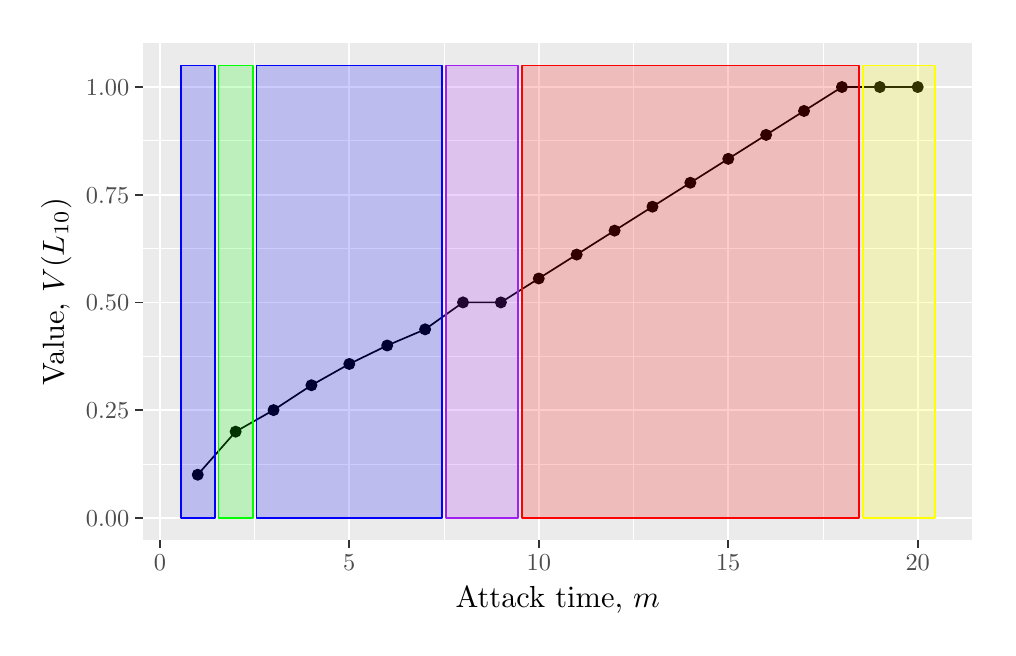
\begin{tikzpicture}[x=1pt,y=1pt]
\definecolor{fillColor}{RGB}{255,255,255}
\path[use as bounding box,fill=fillColor,fill opacity=0.00] (0,0) rectangle (346.90,216.81);
\begin{scope}
\path[clip] (  0.00,  0.00) rectangle (346.90,216.81);
\definecolor{drawColor}{RGB}{255,255,255}
\definecolor{fillColor}{RGB}{255,255,255}

\path[draw=drawColor,line width= 0.6pt,line join=round,line cap=round,fill=fillColor] (  0.00,  0.00) rectangle (346.90,216.81);
\end{scope}
\begin{scope}
\path[clip] ( 41.67, 31.53) rectangle (341.40,211.31);
\definecolor{fillColor}{gray}{0.92}

\path[fill=fillColor] ( 41.67, 31.53) rectangle (341.40,211.31);
\definecolor{drawColor}{RGB}{255,255,255}

\path[draw=drawColor,line width= 0.3pt,line join=round] ( 41.67, 59.16) --
	(341.40, 59.16);

\path[draw=drawColor,line width= 0.3pt,line join=round] ( 41.67, 98.07) --
	(341.40, 98.07);

\path[draw=drawColor,line width= 0.3pt,line join=round] ( 41.67,136.99) --
	(341.40,136.99);

\path[draw=drawColor,line width= 0.3pt,line join=round] ( 41.67,175.90) --
	(341.40,175.90);

\path[draw=drawColor,line width= 0.3pt,line join=round] ( 81.99, 31.53) --
	( 81.99,211.31);

\path[draw=drawColor,line width= 0.3pt,line join=round] (150.45, 31.53) --
	(150.45,211.31);

\path[draw=drawColor,line width= 0.3pt,line join=round] (218.92, 31.53) --
	(218.92,211.31);

\path[draw=drawColor,line width= 0.3pt,line join=round] (287.38, 31.53) --
	(287.38,211.31);

\path[draw=drawColor,line width= 0.6pt,line join=round] ( 41.67, 39.70) --
	(341.40, 39.70);

\path[draw=drawColor,line width= 0.6pt,line join=round] ( 41.67, 78.62) --
	(341.40, 78.62);

\path[draw=drawColor,line width= 0.6pt,line join=round] ( 41.67,117.53) --
	(341.40,117.53);

\path[draw=drawColor,line width= 0.6pt,line join=round] ( 41.67,156.44) --
	(341.40,156.44);

\path[draw=drawColor,line width= 0.6pt,line join=round] ( 41.67,195.36) --
	(341.40,195.36);

\path[draw=drawColor,line width= 0.6pt,line join=round] ( 47.76, 31.53) --
	( 47.76,211.31);

\path[draw=drawColor,line width= 0.6pt,line join=round] (116.22, 31.53) --
	(116.22,211.31);

\path[draw=drawColor,line width= 0.6pt,line join=round] (184.68, 31.53) --
	(184.68,211.31);

\path[draw=drawColor,line width= 0.6pt,line join=round] (253.15, 31.53) --
	(253.15,211.31);

\path[draw=drawColor,line width= 0.6pt,line join=round] (321.61, 31.53) --
	(321.61,211.31);
\definecolor{drawColor}{RGB}{0,0,0}
\definecolor{fillColor}{RGB}{0,0,0}

\path[draw=drawColor,line width= 0.4pt,line join=round,line cap=round,fill=fillColor] (307.92,195.36) circle (  1.96);

\path[draw=drawColor,line width= 0.4pt,line join=round,line cap=round,fill=fillColor] (321.61,195.36) circle (  1.96);

\path[draw=drawColor,line width= 0.4pt,line join=round,line cap=round,fill=fillColor] (184.68,126.18) circle (  1.96);

\path[draw=drawColor,line width= 0.4pt,line join=round,line cap=round,fill=fillColor] (198.38,134.82) circle (  1.96);

\path[draw=drawColor,line width= 0.4pt,line join=round,line cap=round,fill=fillColor] (212.07,143.47) circle (  1.96);

\path[draw=drawColor,line width= 0.4pt,line join=round,line cap=round,fill=fillColor] (225.76,152.12) circle (  1.96);

\path[draw=drawColor,line width= 0.4pt,line join=round,line cap=round,fill=fillColor] (239.45,160.77) circle (  1.96);

\path[draw=drawColor,line width= 0.4pt,line join=round,line cap=round,fill=fillColor] (253.15,169.41) circle (  1.96);

\path[draw=drawColor,line width= 0.4pt,line join=round,line cap=round,fill=fillColor] (266.84,178.06) circle (  1.96);

\path[draw=drawColor,line width= 0.4pt,line join=round,line cap=round,fill=fillColor] (280.53,186.71) circle (  1.96);

\path[draw=drawColor,line width= 0.4pt,line join=round,line cap=round,fill=fillColor] (294.23,195.36) circle (  1.96);

\path[draw=drawColor,line width= 0.4pt,line join=round,line cap=round,fill=fillColor] ( 75.14, 70.83) circle (  1.96);

\path[draw=drawColor,line width= 0.4pt,line join=round,line cap=round,fill=fillColor] (170.99,117.53) circle (  1.96);

\path[draw=drawColor,line width= 0.4pt,line join=round,line cap=round,fill=fillColor] (157.30,117.53) circle (  1.96);

\path[draw=drawColor,line width= 0.4pt,line join=round,line cap=round,fill=fillColor] ( 88.84, 78.62) circle (  1.96);

\path[draw=drawColor,line width= 0.4pt,line join=round,line cap=round,fill=fillColor] (102.53, 87.60) circle (  1.96);

\path[draw=drawColor,line width= 0.4pt,line join=round,line cap=round,fill=fillColor] (116.22, 95.29) circle (  1.96);

\path[draw=drawColor,line width= 0.4pt,line join=round,line cap=round,fill=fillColor] (129.91,101.96) circle (  1.96);

\path[draw=drawColor,line width= 0.4pt,line join=round,line cap=round,fill=fillColor] (143.61,107.80) circle (  1.96);

\path[draw=drawColor,line width= 0.4pt,line join=round,line cap=round,fill=fillColor] ( 61.45, 55.27) circle (  1.96);

\path[draw=drawColor,line width= 0.6pt,line join=round] ( 61.45, 55.27) --
	( 75.14, 70.83) --
	( 88.84, 78.62) --
	(102.53, 87.60) --
	(116.22, 95.29) --
	(129.91,101.96) --
	(143.61,107.80) --
	(157.30,117.53) --
	(170.99,117.53) --
	(184.68,126.18) --
	(198.38,134.82) --
	(212.07,143.47) --
	(225.76,152.12) --
	(239.45,160.77) --
	(253.15,169.41) --
	(266.84,178.06) --
	(280.53,186.71) --
	(294.23,195.36) --
	(307.92,195.36) --
	(321.61,195.36);
\definecolor{drawColor}{RGB}{255,255,0}
\definecolor{fillColor}{RGB}{255,255,0}

\path[draw=drawColor,line width= 0.6pt,line join=round,fill=fillColor,fill opacity=0.20] (301.76, 39.70) rectangle (327.77,203.14);
\definecolor{drawColor}{RGB}{255,0,0}
\definecolor{fillColor}{RGB}{255,0,0}

\path[draw=drawColor,line width= 0.6pt,line join=round,fill=fillColor,fill opacity=0.20] (178.52, 39.70) rectangle (300.39,203.14);
\definecolor{drawColor}{RGB}{160,32,240}
\definecolor{fillColor}{RGB}{160,32,240}

\path[draw=drawColor,line width= 0.6pt,line join=round,fill=fillColor,fill opacity=0.20] (151.14, 39.70) rectangle (177.15,203.14);
\definecolor{drawColor}{RGB}{0,0,255}
\definecolor{fillColor}{RGB}{0,0,255}

\path[draw=drawColor,line width= 0.6pt,line join=round,fill=fillColor,fill opacity=0.20] ( 82.68, 39.70) rectangle (149.77,203.14);
\definecolor{drawColor}{RGB}{0,255,0}
\definecolor{fillColor}{RGB}{0,255,0}

\path[draw=drawColor,line width= 0.6pt,line join=round,fill=fillColor,fill opacity=0.20] ( 68.98, 39.70) rectangle ( 81.31,203.14);
\definecolor{drawColor}{RGB}{0,0,255}
\definecolor{fillColor}{RGB}{0,0,255}

\path[draw=drawColor,line width= 0.6pt,line join=round,fill=fillColor,fill opacity=0.20] ( 55.29, 39.70) rectangle ( 67.61,203.14);
\end{scope}
\begin{scope}
\path[clip] (  0.00,  0.00) rectangle (346.90,216.81);
\definecolor{drawColor}{gray}{0.30}

\node[text=drawColor,anchor=base east,inner sep=0pt, outer sep=0pt, scale=  0.88] at ( 36.72, 36.67) {0.00};

\node[text=drawColor,anchor=base east,inner sep=0pt, outer sep=0pt, scale=  0.88] at ( 36.72, 75.59) {0.25};

\node[text=drawColor,anchor=base east,inner sep=0pt, outer sep=0pt, scale=  0.88] at ( 36.72,114.50) {0.50};

\node[text=drawColor,anchor=base east,inner sep=0pt, outer sep=0pt, scale=  0.88] at ( 36.72,153.41) {0.75};

\node[text=drawColor,anchor=base east,inner sep=0pt, outer sep=0pt, scale=  0.88] at ( 36.72,192.33) {1.00};
\end{scope}
\begin{scope}
\path[clip] (  0.00,  0.00) rectangle (346.90,216.81);
\definecolor{drawColor}{gray}{0.20}

\path[draw=drawColor,line width= 0.6pt,line join=round] ( 38.92, 39.70) --
	( 41.67, 39.70);

\path[draw=drawColor,line width= 0.6pt,line join=round] ( 38.92, 78.62) --
	( 41.67, 78.62);

\path[draw=drawColor,line width= 0.6pt,line join=round] ( 38.92,117.53) --
	( 41.67,117.53);

\path[draw=drawColor,line width= 0.6pt,line join=round] ( 38.92,156.44) --
	( 41.67,156.44);

\path[draw=drawColor,line width= 0.6pt,line join=round] ( 38.92,195.36) --
	( 41.67,195.36);
\end{scope}
\begin{scope}
\path[clip] (  0.00,  0.00) rectangle (346.90,216.81);
\definecolor{drawColor}{gray}{0.20}

\path[draw=drawColor,line width= 0.6pt,line join=round] ( 47.76, 28.78) --
	( 47.76, 31.53);

\path[draw=drawColor,line width= 0.6pt,line join=round] (116.22, 28.78) --
	(116.22, 31.53);

\path[draw=drawColor,line width= 0.6pt,line join=round] (184.68, 28.78) --
	(184.68, 31.53);

\path[draw=drawColor,line width= 0.6pt,line join=round] (253.15, 28.78) --
	(253.15, 31.53);

\path[draw=drawColor,line width= 0.6pt,line join=round] (321.61, 28.78) --
	(321.61, 31.53);
\end{scope}
\begin{scope}
\path[clip] (  0.00,  0.00) rectangle (346.90,216.81);
\definecolor{drawColor}{gray}{0.30}

\node[text=drawColor,anchor=base,inner sep=0pt, outer sep=0pt, scale=  0.88] at ( 47.76, 20.52) {0};

\node[text=drawColor,anchor=base,inner sep=0pt, outer sep=0pt, scale=  0.88] at (116.22, 20.52) {5};

\node[text=drawColor,anchor=base,inner sep=0pt, outer sep=0pt, scale=  0.88] at (184.68, 20.52) {10};

\node[text=drawColor,anchor=base,inner sep=0pt, outer sep=0pt, scale=  0.88] at (253.15, 20.52) {15};

\node[text=drawColor,anchor=base,inner sep=0pt, outer sep=0pt, scale=  0.88] at (321.61, 20.52) {20};
\end{scope}
\begin{scope}
\path[clip] (  0.00,  0.00) rectangle (346.90,216.81);
\definecolor{drawColor}{RGB}{0,0,0}

\node[text=drawColor,anchor=base,inner sep=0pt, outer sep=0pt, scale=  1.10] at (191.53,  7.44) {Attack time, $m$};
\end{scope}
\begin{scope}
\path[clip] (  0.00,  0.00) rectangle (346.90,216.81);
\definecolor{drawColor}{RGB}{0,0,0}

\node[text=drawColor,rotate= 90.00,anchor=base,inner sep=0pt, outer sep=0pt, scale=  1.10] at ( 13.08,121.42) {Value, $V(L_{ 10 })$};
\end{scope}
\end{tikzpicture}

\end{center}
\caption{Value of game on $L_{10}$ with attention drawn to $(10,m)$ split into regions; \textcolor{yellow}{$S_{1}$},\textcolor{red}{$S_{2}$},\textcolor{purple}{$S_{4}$},\textcolor{blue}{$S_{5}$},\textcolor{green}{$S_{3}$}}
\label{Figure:Line 10 value function}
\end{myfigure}

We also note that $S_{2}$ uses the diametric attack in \cite{Papadaki2016}, and so its ambiguity in the time horizon can be resolved using the alteration in \ref{Section:Patrolling games}

\textbf{Bipartite:}

In a bipartite graph, with sets disjoin sets $A$ and $B$ (WLOG assume $|B| \geq |A|$),then the \textit{Bipartite Attack} selects nodes will equal probability from $B$ for a fixed time interval, $I$ (or for the two time intervals, $I$ and $I+1$ with equal probability if $m$ is odd). It has been shown that by the patroller following the attack $V \leq \frac{m}{2|B|}$ as the patroller much alternate between the sets, seeing a potential attack every other time periods(during the attack interval). When $m \geq 2|B|$ this alternating guarantees capture and $V=1$.

On a complete biparitate, $K_{b,b}$ which is a hamiltonian graph, the patroller bound gets a tight lower bound so they show that $V=\frac{m}{2b}$.

\begin{note}
When $m$ is odd, the use of two fixed time intervals $I$ and $I+1$ is made to `balance' the fact that it is possible to see $\frac{m+1}{2}$ possible attacks, but with the offset time intervals two of these only see half a potential attack.
\end{note}

\subsubsection{Conclusion on review of patrolling problem}
While \cite{Alpern2011} introduced the patrolling game and along with \cite{Papadaki2016} solved the game for some of the most common graphical structures, they present no solution for generic graphs and comment that exact solutions to graphs are difficult to find. However with common graph classes solved they have provided a good baseline for our future work, which will continue their theory, discussing new strategies and their applications to a more generalised line graph, called the extended star graph.

\subsection{Review of patrolling problem with random attackers}
\label{Section:Review of patrolling problem with random attackers}
As discussed towards the end of section \ref{Section:Review of Strategic Patrolling games}, it proves quite difficult to find exact solutions to the patrolling game for general graphs. With an aim to develop strategies to the patrolling game on any graph, \cite{Lin2013} first develops a model similar to the patrol game, the patrolling problem, which is only strategic for the patroller and uses stochastic attack time distributions in the infinite time horizon for randomly arriving attackers. They manage to find a near optimal heuristic for the patroller by using Lagrangian relaxation and finding an index, referred to as the fair cost to visit a node, along the lines of those developed by \cite{Whittle1988}. Later they reintroduce the game-theoretic element of a strategic attacker by formulating a normal-form(matrix) game, in which the patroller has only a finite list of strategies, picked to be `appropriately good'.

We now provide a summary of the work done in \cite{Lin2013} with some new notation.

\subsubsection{Problem set-up}
A patrolling problem with random attackers, $G=G(Q,\bm{X},\Lambda,\bm{p},\bm{c})$ is a minimizing problem for the patroller. The parameters of the problem are

\begin{itemize}
\item The graph, $Q=(N,E)$, made of nodes, $N$ ($|N|=n$), joined by edges, $E$, which can be represented by an adjacency matrix, $A$.
\item A vector of attack time distributions, $\bm{X}=(X_{1},...,X_{n})$.
\item A Poisson process arrival rate, $\Lambda$.
\item A vector of node choosing probabilities, $\bm{p}=(p_{1},...,p_{n})$
\item A vector of costs, $\bm{c}=(c_{1},...,c_{n})$.
\end{itemize}

\begin{myfigure}
\begin{center}
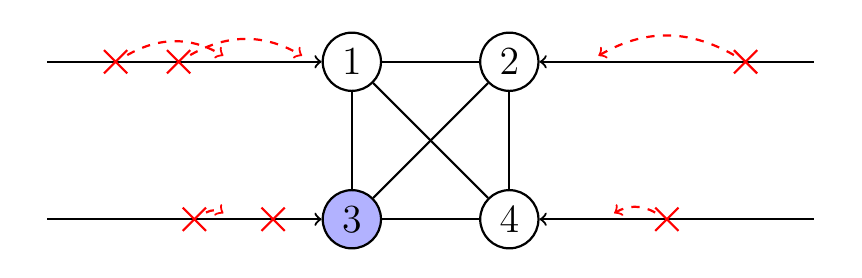
\begin{tikzpicture}[-,auto,node distance=2cm,
                    thick,main node/.style={circle,fill=white,draw,font=\sffamily\Large\bfseries}]

%DRAWING GRAPH
  \node[main node] (1) {$1$};
  \node[main node] (2) [right of=1] {$2$};
  \node[main node,fill=blue!30] (3) [below of=1]  {$3$};
  \node[main node] (4) [below of=2]  {$4$};

  \path[every node/.style={font=\sffamily}]
    (1) edge (2)
        edge (3)
        edge (4)
    (2) edge (3)
        edge (4)
    (3) edge (4);
  
  
%DRAWING ARRIVALS  
  \node (1ArrowStart) [shift={(-4,0)}] at (1) {};
  \draw[->] (1ArrowStart)--(1);
  
  \node[cross=5pt,color=red] (1Cross1) [shift={(-3,0)}] at (1) { };
  \node (1CrossEnd1) [shift={(-1.5,0)}] at (1) {};
  \draw[->,bend left,dashed,color=red] (1Cross1) to (1CrossEnd1);
  \node[cross=5pt,color=red] (1Cross2) [shift={(-2.2,0)}] at (1) { };
  \node (1CrossEnd2) [shift={(-0.5,0)}] at (1) {};
  \draw[->,bend left,dashed,color=red] (1Cross2) to (1CrossEnd2);
  
  \node (2ArrowStart) [shift={(4,0)}] at (2) {};
  \draw[->] (2ArrowStart)--(2);
  
  \node[cross=5pt,color=red] (2Cross1) [shift={(3,0)}] at (2) { };
  \node (2CrossEnd1) [shift={(1,0)}] at (2) {};
  \draw[->,bend right,dashed,color=red] (2Cross1) to (2CrossEnd1);

  \node (3ArrowStart) [shift={(-4,0)}] at (3) {};
  \draw[->] (3ArrowStart)--(3);
  
  \node[cross=5pt,color=red] (3Cross1) [shift={(-2,0)}] at (3) { };
  \node (3CrossEnd1) [shift={(-1.5,0)}] at (3) {};
  \draw[->,bend left,dashed,color=red] (3Cross1) to (3CrossEnd1);
  \node[cross=5pt,color=red] (3Cross1) [shift={(-1,0)}] at (3) { };
  
  \node (4ArrowStart) [shift={(4,0)}] at (4) {};
  \draw[->] (4ArrowStart)--(4);
  
  \node[cross=5pt,color=red] (4Cross1) [shift={(2,0)}] at (4) { };
  \node (4CrossEnd1) [shift={(1.2,0)}] at (4) {};
  \draw[->,bend right,dashed,color=red] (4Cross1) to (4CrossEnd1);
    
\end{tikzpicture}
\end{center}
\caption{Example of $G=(K_{4},\bm{X},\Lambda,\bm{p},\bm{c})$ with patroller currently at node $3$.}
\label{Figure:Example of graph diagram}
\end{myfigure}

The attackers arrive to the system at a rate of $\Lambda$, at which point they pick to attack node $i$ with probability $p_{i}$. They begin their attack immediately, which lasts an amount of time drawn from the nodes attack time distribution, $X_{i}$. The patroller detects all ongoing attacks when arriving at node $i$, the patroller then decides which node to move to and moves there taking unit time to arrive(which can be the current node). Figure \ref{Figure:Example of graph diagram} shows shows an example of the current state of a graph, and figure \ref{Figure:Example of timing for original problem} shows an example of the timing at a node when the patroller arrives after travelling for one unit time along an edge.

By Poisson thinning it is possible to divide the overall Poisson arrival process to individual Poisson arrival processes at each node, with rate $\lambda_{i}=\Lambda p_{i}$. So we can use the single parameter of $\bm{\lambda}=(\lambda_{1},...,\lambda_{n})$, instead of $\Lambda$ and $\bm{p}$.  

\begin{myfigure}
\begin{center}
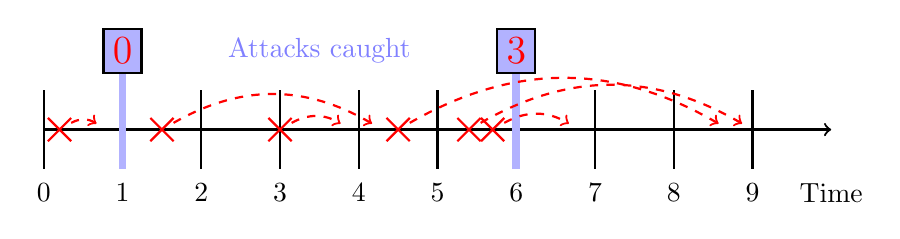
\begin{tikzpicture}[-,auto,node distance=2cm,
                    thick,main node/.style={rectangle,draw,font=\sffamily\Large\bfseries}]

%DRAWING Base line

 \draw[->] (0,0)--(10,0);
 
 \foreach \x in {0,...,9}
 {\draw  (\x,0.5)--(\x,-0.5) ;
  \node (TimeLabel\x) at (\x,-0.8) {$\x$};} 
  
  \node (TimeLabel) at (10,-0.8) {Time};

%Inserting patroller and attackers
  \node[main node,fill=blue!30] (Pat1) at (1,1) {\textcolor{red}{$0$}};
  \draw[color=blue!30,line width=0.1cm] (Pat1)--(1,-0.5);
  
  \node[main node,fill=blue!30] (Pat2) at (6,1) {\textcolor{red}{$3$}};
  \draw[color=blue!30,line width=0.1cm] (Pat2)--(6,-0.5);
  
  \node[cross=5pt,color=red] (AttackStart1) at (0.2,0) {};
  \node (AttackEnd1) at (0.8,0) {};
  \draw[bend left,color=red,->,dashed] (AttackStart1) to (AttackEnd1);
  
  \node[cross=5pt,color=red] (AttackStart2) at (1.5,0) {};
  \node (AttackEnd2) at (4.3,0) {};
  \draw[bend left,color=red,->,dashed] (AttackStart2) to (AttackEnd2);
  
  \node[cross=5pt,color=red] (AttackStart3) at (3,0) {};
  \node (AttackEnd3) at (3.9,0) {};
  \draw[bend left,color=red,->,dashed] (AttackStart3) to (AttackEnd3);
  
  \node[cross=5pt,color=red] (AttackStart4) at (4.5,0) {};
  \node (AttackEnd4) at (8.7,0) {};
  \draw[bend left,color=red,->,dashed] (AttackStart4) to (AttackEnd4);
  
  \node[cross=5pt,color=red] (AttackStart5) at (5.4,0) {};
  \node (AttackEnd5) at (9,0) {};
  \draw[bend left,color=red,->,dashed] (AttackStart5) to (AttackEnd5);
  
  \node[cross=5pt,color=red] (AttackStart6) at (5.7,0) {};
  \node (AttackEnd6) at (6.8,0) {};
  \draw[bend left,color=red,->,dashed] (AttackStart6) to (AttackEnd6);
  
  
  \node (AttacksCaught) at (3.5,1) {\textcolor{blue!50}{Attacks caught}};
       
\end{tikzpicture}
\end{center}
\caption{Example for a given node, when the patroller visits at times, $1,5$.}
\label{Figure:Example of timing for original problem}
\end{myfigure}

We can formulate such a problem as a Markov Decision Process(MDP) with state space, $\Omega= \{\bm{s}=(s_{1},...,s_{n}) \, | \, s_{i}=1,2,... \, \text{ for } i=1,...,n \}$,  where $s_{i}$ denotes the time since the decision to last visit node $i$ was taken. Because the patroller can only visit one node per time period, all $s_{i}$ have distinct values. In particular one $s_{i}$, the current node, has value $1$. We can identify the current node by $l(\bm{s})=\argmin_{i} s_{i}$. The available decisions from state $\bm{s}$ are $\mathcal{A}(\bm{s})=\{j \, | \, A_{l(\bm{s}),j}=1 \}$ and when node $i$ is chosen by the patroller the state transitions to $\phi(\bm{s},i)=\widetilde{\bm{s}}$, where $\widetilde{s}_{i}=1$ and $\widetilde{s}_{j}=s_{j}+1 \; \forall j \neq i$.

Because the future of the process is independent of its past, it is only the current state that matters, the process is a Markov Chain(MC) and hence the patroller's problem is justified as a MDP.

The patroller incurs costs for all attackers able to complete their attacks. When the decision to move to node $i$ is made the cost incurred for the next time period is $C(\bm{s},i)=\sum\limits_{j=1}^{n} C_{j}(\bm{s},i)$ , where $C_{j}(\bm{s},i)$ is the cost at node $j$ choosing to move to node $i$ in the next time period. We have that

\begin{align*}
C_{j}(\bm{s},i)&=c_{j} \lambda_{j} \int_{0}^{s_{j}} P(t-1 < X_{j} \leq t) dt \\
&=c_{j} \lambda_{j} \int_{s_{j}-1}^{s_{j}} P(X_{j} \leq t) dt
\end{align*}

Due to the choice of the patroller moving at unit speed and arriving at the next node one time period later we notice that $C_{j}(\bm{s},i)$ is not dependent on $i$ and that the choice of $i$ affects the future state (and hence future incurred costs)
  
With a countable infinite state space, $\Omega$, problems of finding an optimal policy may exist (See Section 8.10.1 in \cite{Puterman1994}), so to avoid this problem they limit themselves to bounded attack time distributions, $X_{j} \leq B_{j} \in \mathbb{Z}^{+} \forall j $, where

\begin{align}
\label{Equation:Definition of attack time bound}
B_{j} \equiv \min \{ k \, | \, k \in \mathbb{Z}^{+} , P(X_{j} \leq k)=1 \} \equiv \ceil{X_{j}}
\end{align}

Then the cost function remains constant, at $c_{j} \lambda_{j}$, for all $s_{j} \geq B_{j}+1$ and so they restrict the state space to $s_{j} \leq B_{j}+1$ and modify the transitions slightly to $\widetilde{s}_{j}=\min(s_{j}+1,B_{j}+1) \; \forall j \neq i$.

They consider the MDP's objective function to be one which minimizes the long-run average cost incurred. Due to the finite state space the set of policies can be restricted to the class of stationary, deterministic ones $\Pi= \{\pi: \Omega \rightarrow N \, |\,\pi(\bm{s}) \in \mathcal{A}(\bm{s}) \}$ (See Theorem 9.1.8 in \cite{Puterman1994}). The aim is therefore to solve

\begin{align*}
C^{\text{OPT}}(\bm{s}_{0}) \equiv \min\limits_{\pi \in \Pi} \sum\limits_{i=1}^{n} V_{i}(\pi,\bm{s}_{0})
\end{align*}

Where $V_{i}(\pi,\bm{s}_{0})$ is the long-run average cost incurred at node $i$ under the policy, $\pi$, starting from state, $(\bm{s}_{0})$ defined by ,

\begin{align*}
V_{i}(\pi,\bm{s}_{0}) \equiv \lim\limits_{N \rightarrow \infty} \frac{1}{N} \sum\limits_{k=0}^{N-1} C_{i}(\phi^{k}_{\pi}(\bm{s}_{0}),\pi(\phi^{k}_{\pi}(\bm{s}_{0})))
\end{align*}
Where $\phi^{k}_{\pi}(\bm{s}_{0})$ is the state after $k$ transitions starting from $(\bm{s}_{0})$ under the policy $\pi$.

Because the transitions are deterministic and the state space is finite, $\phi^{k}_{\pi}(\bm{s}_{0})$ will repeat and induce a cyclic behaviour under the policy, $\pi$. We will define the patrol pattern to be exactly this, from $\bm{s}_{0}$ let $\bm{s}_{R}$ be the first state which is repeated then define $\psi^{k}_{\pi}=\phi^{k}_{\pi}(\bm{s}_{R})$, so the patrol pattern is $\psi=\{\psi^{k}_{\pi} \, | \, k=0,1,...,K-1 \}$. We say the patrol pattern is of length $K$. We can rewrite the long-run average cost at a node to be

\begin{align}
\label{Equation:Average long run cost via patrol pattern}
V_{i}(\psi)=\frac{1}{K} \sum\limits_{k=0}^{K-1} C_{i}(\psi^{k}_{\pi},\pi(\psi^{k}_{\pi}))
\end{align}

For each policy, $\pi$, and initial state, $\bm{s}_{0}$, a patrol pattern is created and hence, $V_{i}(\pi,\bm{s}_{0})$ is dependent on both the initial state and the policy.

Now $C^{\text{OPT}}(\bm{s}_{0})$ is the optimal cost picking the optimal policy $\pi$, starting from $\bm{s}_{0}$. Now say the graph is connected then, as the objective is the long-run average, we can transition to a new `starting state' and then do the best patrol policy, hence $C^{\text{OPT}}$ does not depend on $\bm{s}_{0}$.

However if the graph is disconnected then it may be impossible to get to the best `starting state' from the initial state and hence different connected components may have different values. Assume the graph is connected.

It is worth noting if $c_{i}=1 \; \forall i$ then we can interpret the long-run average cost, as the probability of not detecting an attack.

Now it is possible, but impractical, to use standard techniques such as value iteration or linear programming to compute the optimal policy and long-run average cost. Therefore a heuristic policy is sought which can be in run in a relatively short space of time, which gets a near optimal policy.

The formulation of the linear program is left to appendix \ref{Appendix:Optimal Solution for a Random Attacker}. These are only used to check the heuristic for small problems where the computation is possible.


\subsubsection{Problem relaxation}
They first relax the issue of the patroller only being able to visit one adjacent node each time period, to the \textit{Multi-Node}(MN) problem, where the patroller can visit multiple nodes each time period, which need not be adjacent. We will denote this class of stationary, deterministic policies as

\begin{align*}
\Pi^{\text{MN}}=\{\pi^{n}: \Omega \rightarrow \bm{\alpha} \, | \alpha_{i}=0,1 \text{ for } i=1,...,n \}
\end{align*}
As this is a relaxed problem for any $\pi \in \Pi$ we can find a $\pi \in \Pi^{\text{MN}}$. Because this problem is easy to solve, the answer is always visit everywhere, it is suggested to place a restriction on the rate of visiting.

Like before $\pi$ will induce a patrol pattern, $\psi^{k}_{\pi}$ with length $K'$. We define the long-run average visit rate at which node, $i$ is visited to be under $\pi$ starting from $\bm{s}_{0}$ as

\begin{align*}
\mu_{i}(\pi_{i},\bm{s}_{0})=\frac{1}{K'} \sum\limits_{k=0}^{K'-1} \pi_{i}(\psi^{k}_{\pi})
\end{align*}

Now we restrict ourselves to having a maximum long-run average visit rate of one. This is known as the \textit{Total-Rate}(TR) constraint. So we restrict ourselves to obey this constraint and to the corresponding set of policies,

\begin{align*}
\Pi^{\text{TR}}=\left\{ \pi \in \Pi^{\text{MN}} \, \bigg| \, \sum\limits_{i=1}^{n} \mu_{i}(\pi_{i},\bm{s}_{0}) \leq 1 \, , \, \forall \bm{s}_{0} \in \Omega \right\}
\end{align*}

Again this is still a relaxation and any $\pi \in \Pi$ has a $\pi \in \Pi^{\text{TR}}$.

\begin{note}
The dependency on the initial state, $\bm{s}_{0}$, is dropped as even though $V_{i}(\pi,\bm{s}_{0})$ depends on it, the long-run average cost does not. We will similarly drop the notation on the long-run visit rate, using $\mu_{i}(\pi)$ instead.
\end{note}

Secondly they relax the TR problem even further by introducing the constraint as a Lagrangian multiplier, $\omega \geq 0$, to form

\begin{align*}
C(\omega) & \equiv \min\limits_{\pi \in \Pi^{\text{MN}}} \left(\sum\limits_{i=1}^{n} V_{i}(\pi) + \omega \left(\sum\limits_{i=1}^{n} \mu_{i}(\pi) -1\right) \right) \\
&= \min\limits_{\pi \in \Pi^{\text{MN}}} \sum\limits_{i=1}^{n} \left(V_{i}(\pi) + \omega \mu_{i}(\pi)\right)  -\omega \\
& = \sum\limits_{i=1}^{n} \min\limits_{\pi \in \Pi^{\text{MN}}} (V_{i}(\pi) +\omega\mu_{i}(\pi)) -\omega \\
& \equiv \sum\limits_{i}^{n} C_{i}(\omega) -\omega
\end{align*}

Where the last equality holds as the sum is finite and $\pi \in \Pi$ can make decisions about node $i$ independent of all other nodes. This means the Lagrangian relaxation separates the problem into $n$ individual node problems, where node $i$'s problem is

\begin{align*}
C_{i}(\omega) \equiv \min\limits_{\pi_{i} \in \Pi^{\text{MN}}_{i}} \left(V_{i}(\pi_{i}) + \omega \mu_{i}(\pi_{i})\right)
\end{align*}

The Lagrangian multiplier, $\omega$, can be seen as \text{service charge} to visit the node.

This formulation means that $C^{\text{TR}} \geq C(\omega)$, hence $C^{\text{OPT}} \geq C^{\text{TR}} \geq C(\omega)$.

\subsubsection{Single-node problem}

Focusing on the separated, single node problem is equivalent to deciding when to visit the node. We shall remove node subscript, $i$, for ease of reading. Each time has a binary decision, visit or wait. Because we are only considering stationary, deterministic policies, the optimal action of when to visit remains constant and the optimal policy will be one that visits every, $k=1,2,....$ periods (possibly never visiting). Such a policy gives us an expected number of arrivals who finish before we visit of

\begin{align*}
\lambda \int_{0}^{k} P(X \leq k-t) dt= \lambda \int_{0}^{k} P(X \leq t) dt
\end{align*}

Each successful attack costs $c$ and the visit costs us $\omega$ and this cycle is of length $k$ so the long-run average cost is

\begin{align*}
f(k) \equiv \frac{c \lambda \int_{0}^{k} P(X \leq t) dt + \omega}{k}
\end{align*}

Thus solving the single node problem is equivalent to minimizing $f(k)$, by setting $f(k) = f(k+1)$ we can find the cost that makes the patroller indifferent between visiting every $k$ and $k+1$ time units. This solution helps us characterise the optimal policy that minimizes $f(k)$ by the index,

\begin{align*}
W(k) \equiv c \lambda \left( k \int_{k}^{k+1} P(x \leq t) dt - \int_{0}^{k} P(x \leq t) dt \right)
\end{align*}

We have $W(0)=0$ and as $X$ is bounded by $B$, we have for $k \geq B$ that $W(k)= c \lambda E[X]$.

\begin{theorem}[Single node optimal policy]
\label{Theorem:Single node optimal policy}
\begin{itemize}
\item[a)] $W(k)$ is non-decreasing in $k$.
\item[b)] If $\omega \in [W(k-1),W(k)]$ then it is optimal to visit the node once every $k$ time periods, for $k=1,2,...$
\item[c)] Moreover if $\omega \geq c \lambda E[X]$ it is never optimal to visit the node.
\end{itemize}
\end{theorem}

Because the patroller will only visit every $k$ time periods if $\omega \in [W(k-1),w(k)]$, one can think of $W(k)$ as the maximum service charge the node is willing to pay to be visited by the patroller. This $W(k)$ is the \textit{fair service charge} for the node that wants to be visited every $k$ time periods.  

This motivates a simple Index Heuristic(IH) based on the optimal solution to the single node problem, by reinserting the node subscript, we suggest an index of

\begin{align*}
W_{i}(\bm{s}) \equiv c_{i} \lambda_{i} \left(s_{i} \int_{s_{i}}^{s_{i}+1} P(X_{i} \leq t) dt - \int_{0}^{s_{i}} P(X_{i} \leq t) dt \right)
\end{align*}

The IH computes the index for all adjacent nodes (including the current node) from the state $\bm{s}$ and moves to the node with the highest index. In the cases of ties in indices, they are broken arbitrarily, that is the patroller services the node with the highest fair service charge.

\subsubsection{More heuristics}
The IH is simplistic and short sighted, as it only looks at servicing the node which is demanding service the most in a one-step fashion, it is suggested in \cite{Lin2013} to use look-ahead windows and then depth.

Suppose instead of looking at only the next time period, we looked ahead $l$ steps, then we have all patroller paths of length $l$ from the current position, to decide amongst the paths we can aggregate the index for all the times we visit nodes along the path. Then the choice for the next node is the first node in the path with the highest aggregate index reward. Such a heuristic is called the \textit{Index Reward Heuristic}(IRH). The IRH policy, will induce some patrol pattern, $\psi_{IRH}$, whose long-run average can be found using equation \ref{Equation:Average long run cost via patrol pattern}.

Another way of interpreting the index is as a penalty for not visiting a node, rather than a reward for visiting one. Again by using a look-ahead window of length $l$ the patroller can decide the next node by looking at all paths of length $l$ from the current node, and then aggregate the indices of all nodes for all the time-steps they are not visited in. Then the choice for the next node is the first node of the paths with the lowest aggregate penalty. Such a heuristic is called the \textit{Index Penalty Heuristic}(IPH). The IPH policy, $\pi_{IPH}$, will induce some patrol pattern which again can be evaluated using the equation

\begin{note}
We only use the aggregate reward/penalty to determine the next node, then we repeat the process, we do not follow the path.
\end{note}

A natural question to ask is; does increasing the look-ahead window improve the heuristic. The answer is no, as $l$ and $l+1$ may return two distinct patrol patterns, with $l$'s patrol pattern performing better than $l+1$'s. They define the IRH/IPH at depth $d$, IRH($d$)/IPH($d$), to be the IRH/IPH used with look-ahead windows $l \leq d$ and simply using the best look-ahead window, ensuring that they are nested and only improve with increasing depth.

\begin{note}
IRH($1$) $\equiv$ IPH($1$) $\equiv$ IH
\end{note}

The numerical results of these heuristics can be found in Section 3.4 in \citep{Lin2013}. A key result of the study, that we will look at later is that IPH seems to outperform IRH on the Complete and Line graph.

\section{Patrolling games}
\label{Section:Patrolling games}

\subsection{Issue and correction of the diametric bound}
\label{Section:Issue and correction of the diametric bound}
We now state Lemma 9 in \cite{Alpern2011} as the diametric bound, the attackers bound by attacking randomly throughout time at the diametric nodes.

\begin{lemma}[Diametric bound]
$V \leq \max \left\{ \frac{1}{2},\frac{m}{\raisebox{-0.5ex}{$\scriptstyle 2 \bar{d}$}} \right\}$, guaranteed by the diametric attack.
\end{lemma}

We will now look at an issue with the diametric bound when $\bar{d} < m \leq 2 \bar{d}$, so we are dealing with the bound $V \leq \frac{m}{\raisebox{-0.5ex}{$\scriptstyle 2 \bar{d}$}}$. The result of the lemma states with ambiguity that this holds for large $m$ and $T$, however the results are used for smaller $T$ such as in Theorem 16 in \citep{Alpern2011}. We will analyse this issue of `large' $T$,  and present a more concrete conclusion on conditions for which $T$ must take in order to use this bound. We will then present an altered diametric attack, which can further help to reduce the conditions on $T$ for the same bound.

The diametric attack has the attacker start at two diametrical nodes with equal probability and then choosing a starting attack time, $\tau=0,1...,T-m$ again with equal probability. Hence it can be thought of as the attacker making $2(T-m+1)$ attacks each with equal probability. To see how the patroller can do against this attacking strategy, we can consider a simple oscillatory strategy, going back and forth between the diametrical nodes, and see how many potential attacks are captured.

\begin{example}[Issue with the diametric bound]
Consider the game $(Q=L_{5},T=20,m=6)$ so $m=6 >\bar{d}=4$, then under the diametric attack the attacker has $30$ attacks, starting at $0,...,14$ at nodes $1$ and $5$. If the patroller oscillates between diametric points they capture
$1+5+6+6+4=22$ attacks out of $2(20-6+1)=30$ attacks, for a capture chance of $V=\frac{11}{15}$, which is greater than diametric bound $\frac{3}{4}$.
\end{example}

We could now consider delaying the patroller initially to get a better number of attacks, e.g. delaying in the counter example to leave at time $2$ instead of $0$ gives $3+6+6+6+2=23$. In fact it is best to delay yourself to leave at time $m-\bar{d}-1$. This can be seen in appendix \ref{Appendix:Proof of diametric waiting time}.

This means the patroller will capture, by oscillating,

\begin{align*}
&\underbrace{m-\bar{d}}_{\text{Waiting initially}} + \underbrace{\pospart{m \times \left( M +1 \right)}}_{\text{Visits which get exactly } m \text{ attacks}} \\
&+ \underbrace{\pospart{T- \left( m-1 + \left(M +1 \right) \bar{d} \right)}+\pospart{T- \left( m-1 + \left(M +2 \right) \bar{d} \right)}}_{\text{Penultimate and final node visits}} 
\end{align*}

Where, $M=\floor{\frac{T-2m+1}{\bar{d}}}$, is the number of nodes after the two initial visits getting exactly $m$ of the potential attacks, an exact derivation of this formula is left to appendix \ref{Appendix:Proof of diametric waiting time}.

The key point is that the upper bound given by the diametric attack is dependent on $T$. An example is given in Figure \ref{Figure:Example of upper bound achieved by diametric attack} which shows that for some $T$ as in Lemma \ref{Lemma:Condition on time horizon for diametric bound to hold} and as the finite time horizon becomes infinite the corrected bound reaches the suggested bound in \cite{Alpern2011}.

\begin{lemma}[Condition on $T$ for bound to hold]
\label{Lemma:Condition on time horizon for diametric bound to hold}
When $T=m-1+(k+1)\bar{d}$ for some $k \in \mathbb{N}_{0}$ then the diametric bound holds. Furthermore as $T \rightarrow \infty$ then the diametric bound holds and moreover the errors are maximal when $T=2m-1+(k+1)\bar{d}$ for some $k \in \mathbb{N}_{0}$ with an error, inversely proportional to the time horizon, explicitly $\frac{m\bar{d}-(m-\bar{d})^{2}}{2\bar{d}(m+(k+1)\bar{d})}=\mathcal{O}(\frac{1}{T})$
\end{lemma}

For proof see Appendix \ref{Appendix:Proof of conditions on T for diametric attack}

\begin{myfigure}

%% Created by tikzDevice version 0.10.1 on 2017-11-09 12:03:49
% !TEX encoding = UTF-8 Unicode
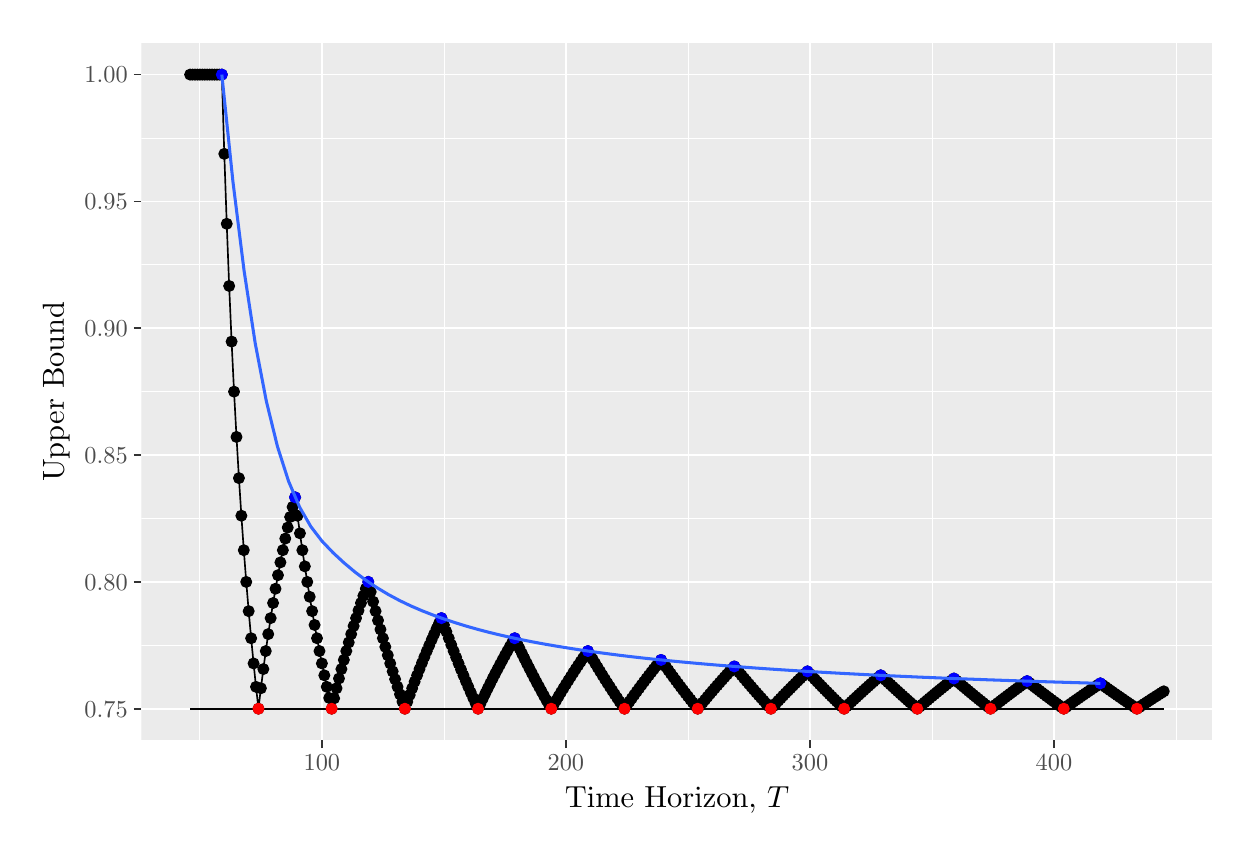
\begin{tikzpicture}[x=1pt,y=1pt]
\definecolor{fillColor}{RGB}{255,255,255}
\path[use as bounding box,fill=fillColor,fill opacity=0.00] (0,0) rectangle (433.62,289.08);
\begin{scope}
\path[clip] (  0.00,  0.00) rectangle (433.62,289.08);
\definecolor{drawColor}{RGB}{255,255,255}
\definecolor{fillColor}{RGB}{255,255,255}

\path[draw=drawColor,line width= 0.6pt,line join=round,line cap=round,fill=fillColor] (  0.00,  0.00) rectangle (433.62,289.08);
\end{scope}
\begin{scope}
\path[clip] ( 41.11, 31.53) rectangle (428.12,283.58);
\definecolor{fillColor}{gray}{0.92}

\path[fill=fillColor] ( 41.11, 31.53) rectangle (428.12,283.58);
\definecolor{drawColor}{RGB}{255,255,255}

\path[draw=drawColor,line width= 0.3pt,line join=round] ( 41.11, 65.90) --
	(428.12, 65.90);

\path[draw=drawColor,line width= 0.3pt,line join=round] ( 41.11,111.73) --
	(428.12,111.73);

\path[draw=drawColor,line width= 0.3pt,line join=round] ( 41.11,157.56) --
	(428.12,157.56);

\path[draw=drawColor,line width= 0.3pt,line join=round] ( 41.11,203.38) --
	(428.12,203.38);

\path[draw=drawColor,line width= 0.3pt,line join=round] ( 41.11,249.21) --
	(428.12,249.21);

\path[draw=drawColor,line width= 0.3pt,line join=round] ( 62.23, 31.53) --
	( 62.23,283.58);

\path[draw=drawColor,line width= 0.3pt,line join=round] (150.41, 31.53) --
	(150.41,283.58);

\path[draw=drawColor,line width= 0.3pt,line join=round] (238.58, 31.53) --
	(238.58,283.58);

\path[draw=drawColor,line width= 0.3pt,line join=round] (326.76, 31.53) --
	(326.76,283.58);

\path[draw=drawColor,line width= 0.3pt,line join=round] (414.94, 31.53) --
	(414.94,283.58);

\path[draw=drawColor,line width= 0.6pt,line join=round] ( 41.11, 42.99) --
	(428.12, 42.99);

\path[draw=drawColor,line width= 0.6pt,line join=round] ( 41.11, 88.81) --
	(428.12, 88.81);

\path[draw=drawColor,line width= 0.6pt,line join=round] ( 41.11,134.64) --
	(428.12,134.64);

\path[draw=drawColor,line width= 0.6pt,line join=round] ( 41.11,180.47) --
	(428.12,180.47);

\path[draw=drawColor,line width= 0.6pt,line join=round] ( 41.11,226.30) --
	(428.12,226.30);

\path[draw=drawColor,line width= 0.6pt,line join=round] ( 41.11,272.12) --
	(428.12,272.12);

\path[draw=drawColor,line width= 0.6pt,line join=round] (106.32, 31.53) --
	(106.32,283.58);

\path[draw=drawColor,line width= 0.6pt,line join=round] (194.49, 31.53) --
	(194.49,283.58);

\path[draw=drawColor,line width= 0.6pt,line join=round] (282.67, 31.53) --
	(282.67,283.58);

\path[draw=drawColor,line width= 0.6pt,line join=round] (370.85, 31.53) --
	(370.85,283.58);
\definecolor{drawColor}{RGB}{0,0,0}
\definecolor{fillColor}{RGB}{0,0,0}

\path[draw=drawColor,line width= 0.4pt,line join=round,line cap=round,fill=fillColor] ( 58.70,272.12) circle (  1.96);

\path[draw=drawColor,line width= 0.4pt,line join=round,line cap=round,fill=fillColor] ( 59.58,272.12) circle (  1.96);

\path[draw=drawColor,line width= 0.4pt,line join=round,line cap=round,fill=fillColor] ( 60.47,272.12) circle (  1.96);

\path[draw=drawColor,line width= 0.4pt,line join=round,line cap=round,fill=fillColor] ( 61.35,272.12) circle (  1.96);

\path[draw=drawColor,line width= 0.4pt,line join=round,line cap=round,fill=fillColor] ( 62.23,272.12) circle (  1.96);

\path[draw=drawColor,line width= 0.4pt,line join=round,line cap=round,fill=fillColor] ( 63.11,272.12) circle (  1.96);

\path[draw=drawColor,line width= 0.4pt,line join=round,line cap=round,fill=fillColor] ( 63.99,272.12) circle (  1.96);

\path[draw=drawColor,line width= 0.4pt,line join=round,line cap=round,fill=fillColor] ( 64.87,272.12) circle (  1.96);

\path[draw=drawColor,line width= 0.4pt,line join=round,line cap=round,fill=fillColor] ( 65.76,272.12) circle (  1.96);

\path[draw=drawColor,line width= 0.4pt,line join=round,line cap=round,fill=fillColor] ( 66.64,272.12) circle (  1.96);

\path[draw=drawColor,line width= 0.4pt,line join=round,line cap=round,fill=fillColor] ( 67.52,272.12) circle (  1.96);

\path[draw=drawColor,line width= 0.4pt,line join=round,line cap=round,fill=fillColor] ( 68.40,272.12) circle (  1.96);

\path[draw=drawColor,line width= 0.4pt,line join=round,line cap=round,fill=fillColor] ( 69.28,272.12) circle (  1.96);

\path[draw=drawColor,line width= 0.4pt,line join=round,line cap=round,fill=fillColor] ( 70.16,272.12) circle (  1.96);

\path[draw=drawColor,line width= 0.4pt,line join=round,line cap=round,fill=fillColor] ( 71.05,243.48) circle (  1.96);

\path[draw=drawColor,line width= 0.4pt,line join=round,line cap=round,fill=fillColor] ( 71.93,218.21) circle (  1.96);

\path[draw=drawColor,line width= 0.4pt,line join=round,line cap=round,fill=fillColor] ( 72.81,195.74) circle (  1.96);

\path[draw=drawColor,line width= 0.4pt,line join=round,line cap=round,fill=fillColor] ( 73.69,175.65) circle (  1.96);

\path[draw=drawColor,line width= 0.4pt,line join=round,line cap=round,fill=fillColor] ( 74.57,157.56) circle (  1.96);

\path[draw=drawColor,line width= 0.4pt,line join=round,line cap=round,fill=fillColor] ( 75.46,141.19) circle (  1.96);

\path[draw=drawColor,line width= 0.4pt,line join=round,line cap=round,fill=fillColor] ( 76.34,126.31) circle (  1.96);

\path[draw=drawColor,line width= 0.4pt,line join=round,line cap=round,fill=fillColor] ( 77.22,112.72) circle (  1.96);

\path[draw=drawColor,line width= 0.4pt,line join=round,line cap=round,fill=fillColor] ( 78.10,100.27) circle (  1.96);

\path[draw=drawColor,line width= 0.4pt,line join=round,line cap=round,fill=fillColor] ( 78.98, 88.81) circle (  1.96);

\path[draw=drawColor,line width= 0.4pt,line join=round,line cap=round,fill=fillColor] ( 79.86, 78.24) circle (  1.96);

\path[draw=drawColor,line width= 0.4pt,line join=round,line cap=round,fill=fillColor] ( 80.75, 68.45) circle (  1.96);

\path[draw=drawColor,line width= 0.4pt,line join=round,line cap=round,fill=fillColor] ( 81.63, 59.35) circle (  1.96);

\path[draw=drawColor,line width= 0.4pt,line join=round,line cap=round,fill=fillColor] ( 82.51, 50.89) circle (  1.96);

\path[draw=drawColor,line width= 0.4pt,line join=round,line cap=round,fill=fillColor] ( 83.39, 42.99) circle (  1.96);

\path[draw=drawColor,line width= 0.4pt,line join=round,line cap=round,fill=fillColor] ( 84.27, 50.38) circle (  1.96);

\path[draw=drawColor,line width= 0.4pt,line join=round,line cap=round,fill=fillColor] ( 85.16, 57.31) circle (  1.96);

\path[draw=drawColor,line width= 0.4pt,line join=round,line cap=round,fill=fillColor] ( 86.04, 63.82) circle (  1.96);

\path[draw=drawColor,line width= 0.4pt,line join=round,line cap=round,fill=fillColor] ( 86.92, 69.94) circle (  1.96);

\path[draw=drawColor,line width= 0.4pt,line join=round,line cap=round,fill=fillColor] ( 87.80, 75.72) circle (  1.96);

\path[draw=drawColor,line width= 0.4pt,line join=round,line cap=round,fill=fillColor] ( 88.68, 81.18) circle (  1.96);

\path[draw=drawColor,line width= 0.4pt,line join=round,line cap=round,fill=fillColor] ( 89.56, 86.34) circle (  1.96);

\path[draw=drawColor,line width= 0.4pt,line join=round,line cap=round,fill=fillColor] ( 90.45, 91.23) circle (  1.96);

\path[draw=drawColor,line width= 0.4pt,line join=round,line cap=round,fill=fillColor] ( 91.33, 95.86) circle (  1.96);

\path[draw=drawColor,line width= 0.4pt,line join=round,line cap=round,fill=fillColor] ( 92.21,100.27) circle (  1.96);

\path[draw=drawColor,line width= 0.4pt,line join=round,line cap=round,fill=fillColor] ( 93.09,104.46) circle (  1.96);

\path[draw=drawColor,line width= 0.4pt,line join=round,line cap=round,fill=fillColor] ( 93.97,108.45) circle (  1.96);

\path[draw=drawColor,line width= 0.4pt,line join=round,line cap=round,fill=fillColor] ( 94.85,112.26) circle (  1.96);

\path[draw=drawColor,line width= 0.4pt,line join=round,line cap=round,fill=fillColor] ( 95.74,115.89) circle (  1.96);

\path[draw=drawColor,line width= 0.4pt,line join=round,line cap=round,fill=fillColor] ( 96.62,119.37) circle (  1.96);

\path[draw=drawColor,line width= 0.4pt,line join=round,line cap=round,fill=fillColor] ( 97.50,112.72) circle (  1.96);

\path[draw=drawColor,line width= 0.4pt,line join=round,line cap=round,fill=fillColor] ( 98.38,106.37) circle (  1.96);

\path[draw=drawColor,line width= 0.4pt,line join=round,line cap=round,fill=fillColor] ( 99.26,100.27) circle (  1.96);

\path[draw=drawColor,line width= 0.4pt,line join=round,line cap=round,fill=fillColor] (100.15, 94.43) circle (  1.96);

\path[draw=drawColor,line width= 0.4pt,line join=round,line cap=round,fill=fillColor] (101.03, 88.81) circle (  1.96);

\path[draw=drawColor,line width= 0.4pt,line join=round,line cap=round,fill=fillColor] (101.91, 83.42) circle (  1.96);

\path[draw=drawColor,line width= 0.4pt,line join=round,line cap=round,fill=fillColor] (102.79, 78.24) circle (  1.96);

\path[draw=drawColor,line width= 0.4pt,line join=round,line cap=round,fill=fillColor] (103.67, 73.25) circle (  1.96);

\path[draw=drawColor,line width= 0.4pt,line join=round,line cap=round,fill=fillColor] (104.55, 68.45) circle (  1.96);

\path[draw=drawColor,line width= 0.4pt,line join=round,line cap=round,fill=fillColor] (105.44, 63.82) circle (  1.96);

\path[draw=drawColor,line width= 0.4pt,line join=round,line cap=round,fill=fillColor] (106.32, 59.35) circle (  1.96);

\path[draw=drawColor,line width= 0.4pt,line join=round,line cap=round,fill=fillColor] (107.20, 55.05) circle (  1.96);

\path[draw=drawColor,line width= 0.4pt,line join=round,line cap=round,fill=fillColor] (108.08, 50.89) circle (  1.96);

\path[draw=drawColor,line width= 0.4pt,line join=round,line cap=round,fill=fillColor] (108.96, 46.87) circle (  1.96);

\path[draw=drawColor,line width= 0.4pt,line join=round,line cap=round,fill=fillColor] (109.84, 42.99) circle (  1.96);

\path[draw=drawColor,line width= 0.4pt,line join=round,line cap=round,fill=fillColor] (110.73, 46.74) circle (  1.96);

\path[draw=drawColor,line width= 0.4pt,line join=round,line cap=round,fill=fillColor] (111.61, 50.38) circle (  1.96);

\path[draw=drawColor,line width= 0.4pt,line join=round,line cap=round,fill=fillColor] (112.49, 53.90) circle (  1.96);

\path[draw=drawColor,line width= 0.4pt,line join=round,line cap=round,fill=fillColor] (113.37, 57.31) circle (  1.96);

\path[draw=drawColor,line width= 0.4pt,line join=round,line cap=round,fill=fillColor] (114.25, 60.61) circle (  1.96);

\path[draw=drawColor,line width= 0.4pt,line join=round,line cap=round,fill=fillColor] (115.14, 63.82) circle (  1.96);

\path[draw=drawColor,line width= 0.4pt,line join=round,line cap=round,fill=fillColor] (116.02, 66.93) circle (  1.96);

\path[draw=drawColor,line width= 0.4pt,line join=round,line cap=round,fill=fillColor] (116.90, 69.94) circle (  1.96);

\path[draw=drawColor,line width= 0.4pt,line join=round,line cap=round,fill=fillColor] (117.78, 72.87) circle (  1.96);

\path[draw=drawColor,line width= 0.4pt,line join=round,line cap=round,fill=fillColor] (118.66, 75.72) circle (  1.96);

\path[draw=drawColor,line width= 0.4pt,line join=round,line cap=round,fill=fillColor] (119.54, 78.49) circle (  1.96);

\path[draw=drawColor,line width= 0.4pt,line join=round,line cap=round,fill=fillColor] (120.43, 81.18) circle (  1.96);

\path[draw=drawColor,line width= 0.4pt,line join=round,line cap=round,fill=fillColor] (121.31, 83.79) circle (  1.96);

\path[draw=drawColor,line width= 0.4pt,line join=round,line cap=round,fill=fillColor] (122.19, 86.34) circle (  1.96);

\path[draw=drawColor,line width= 0.4pt,line join=round,line cap=round,fill=fillColor] (123.07, 88.81) circle (  1.96);

\path[draw=drawColor,line width= 0.4pt,line join=round,line cap=round,fill=fillColor] (123.95, 85.20) circle (  1.96);

\path[draw=drawColor,line width= 0.4pt,line join=round,line cap=round,fill=fillColor] (124.83, 81.67) circle (  1.96);

\path[draw=drawColor,line width= 0.4pt,line join=round,line cap=round,fill=fillColor] (125.72, 78.24) circle (  1.96);

\path[draw=drawColor,line width= 0.4pt,line join=round,line cap=round,fill=fillColor] (126.60, 74.89) circle (  1.96);

\path[draw=drawColor,line width= 0.4pt,line join=round,line cap=round,fill=fillColor] (127.48, 71.63) circle (  1.96);

\path[draw=drawColor,line width= 0.4pt,line join=round,line cap=round,fill=fillColor] (128.36, 68.45) circle (  1.96);

\path[draw=drawColor,line width= 0.4pt,line join=round,line cap=round,fill=fillColor] (129.24, 65.34) circle (  1.96);

\path[draw=drawColor,line width= 0.4pt,line join=round,line cap=round,fill=fillColor] (130.13, 62.31) circle (  1.96);

\path[draw=drawColor,line width= 0.4pt,line join=round,line cap=round,fill=fillColor] (131.01, 59.35) circle (  1.96);

\path[draw=drawColor,line width= 0.4pt,line join=round,line cap=round,fill=fillColor] (131.89, 56.47) circle (  1.96);

\path[draw=drawColor,line width= 0.4pt,line join=round,line cap=round,fill=fillColor] (132.77, 53.64) circle (  1.96);

\path[draw=drawColor,line width= 0.4pt,line join=round,line cap=round,fill=fillColor] (133.65, 50.89) circle (  1.96);

\path[draw=drawColor,line width= 0.4pt,line join=round,line cap=round,fill=fillColor] (134.53, 48.20) circle (  1.96);

\path[draw=drawColor,line width= 0.4pt,line join=round,line cap=round,fill=fillColor] (135.42, 45.56) circle (  1.96);

\path[draw=drawColor,line width= 0.4pt,line join=round,line cap=round,fill=fillColor] (136.30, 42.99) circle (  1.96);

\path[draw=drawColor,line width= 0.4pt,line join=round,line cap=round,fill=fillColor] (137.18, 45.51) circle (  1.96);

\path[draw=drawColor,line width= 0.4pt,line join=round,line cap=round,fill=fillColor] (138.06, 47.97) circle (  1.96);

\path[draw=drawColor,line width= 0.4pt,line join=round,line cap=round,fill=fillColor] (138.94, 50.38) circle (  1.96);

\path[draw=drawColor,line width= 0.4pt,line join=round,line cap=round,fill=fillColor] (139.82, 52.74) circle (  1.96);

\path[draw=drawColor,line width= 0.4pt,line join=round,line cap=round,fill=fillColor] (140.71, 55.05) circle (  1.96);

\path[draw=drawColor,line width= 0.4pt,line join=round,line cap=round,fill=fillColor] (141.59, 57.31) circle (  1.96);

\path[draw=drawColor,line width= 0.4pt,line join=round,line cap=round,fill=fillColor] (142.47, 59.52) circle (  1.96);

\path[draw=drawColor,line width= 0.4pt,line join=round,line cap=round,fill=fillColor] (143.35, 61.69) circle (  1.96);

\path[draw=drawColor,line width= 0.4pt,line join=round,line cap=round,fill=fillColor] (144.23, 63.82) circle (  1.96);

\path[draw=drawColor,line width= 0.4pt,line join=round,line cap=round,fill=fillColor] (145.12, 65.90) circle (  1.96);

\path[draw=drawColor,line width= 0.4pt,line join=round,line cap=round,fill=fillColor] (146.00, 67.94) circle (  1.96);

\path[draw=drawColor,line width= 0.4pt,line join=round,line cap=round,fill=fillColor] (146.88, 69.94) circle (  1.96);

\path[draw=drawColor,line width= 0.4pt,line join=round,line cap=round,fill=fillColor] (147.76, 71.91) circle (  1.96);

\path[draw=drawColor,line width= 0.4pt,line join=round,line cap=round,fill=fillColor] (148.64, 73.83) circle (  1.96);

\path[draw=drawColor,line width= 0.4pt,line join=round,line cap=round,fill=fillColor] (149.52, 75.72) circle (  1.96);

\path[draw=drawColor,line width= 0.4pt,line join=round,line cap=round,fill=fillColor] (150.41, 73.25) circle (  1.96);

\path[draw=drawColor,line width= 0.4pt,line join=round,line cap=round,fill=fillColor] (151.29, 70.83) circle (  1.96);

\path[draw=drawColor,line width= 0.4pt,line join=round,line cap=round,fill=fillColor] (152.17, 68.45) circle (  1.96);

\path[draw=drawColor,line width= 0.4pt,line join=round,line cap=round,fill=fillColor] (153.05, 66.11) circle (  1.96);

\path[draw=drawColor,line width= 0.4pt,line join=round,line cap=round,fill=fillColor] (153.93, 63.82) circle (  1.96);

\path[draw=drawColor,line width= 0.4pt,line join=round,line cap=round,fill=fillColor] (154.82, 61.57) circle (  1.96);

\path[draw=drawColor,line width= 0.4pt,line join=round,line cap=round,fill=fillColor] (155.70, 59.35) circle (  1.96);

\path[draw=drawColor,line width= 0.4pt,line join=round,line cap=round,fill=fillColor] (156.58, 57.18) circle (  1.96);

\path[draw=drawColor,line width= 0.4pt,line join=round,line cap=round,fill=fillColor] (157.46, 55.05) circle (  1.96);

\path[draw=drawColor,line width= 0.4pt,line join=round,line cap=round,fill=fillColor] (158.34, 52.95) circle (  1.96);

\path[draw=drawColor,line width= 0.4pt,line join=round,line cap=round,fill=fillColor] (159.22, 50.89) circle (  1.96);

\path[draw=drawColor,line width= 0.4pt,line join=round,line cap=round,fill=fillColor] (160.11, 48.86) circle (  1.96);

\path[draw=drawColor,line width= 0.4pt,line join=round,line cap=round,fill=fillColor] (160.99, 46.87) circle (  1.96);

\path[draw=drawColor,line width= 0.4pt,line join=round,line cap=round,fill=fillColor] (161.87, 44.91) circle (  1.96);

\path[draw=drawColor,line width= 0.4pt,line join=round,line cap=round,fill=fillColor] (162.75, 42.99) circle (  1.96);

\path[draw=drawColor,line width= 0.4pt,line join=round,line cap=round,fill=fillColor] (163.63, 44.88) circle (  1.96);

\path[draw=drawColor,line width= 0.4pt,line join=round,line cap=round,fill=fillColor] (164.51, 46.74) circle (  1.96);

\path[draw=drawColor,line width= 0.4pt,line join=round,line cap=round,fill=fillColor] (165.40, 48.58) circle (  1.96);

\path[draw=drawColor,line width= 0.4pt,line join=round,line cap=round,fill=fillColor] (166.28, 50.38) circle (  1.96);

\path[draw=drawColor,line width= 0.4pt,line join=round,line cap=round,fill=fillColor] (167.16, 52.15) circle (  1.96);

\path[draw=drawColor,line width= 0.4pt,line join=round,line cap=round,fill=fillColor] (168.04, 53.90) circle (  1.96);

\path[draw=drawColor,line width= 0.4pt,line join=round,line cap=round,fill=fillColor] (168.92, 55.62) circle (  1.96);

\path[draw=drawColor,line width= 0.4pt,line join=round,line cap=round,fill=fillColor] (169.81, 57.31) circle (  1.96);

\path[draw=drawColor,line width= 0.4pt,line join=round,line cap=round,fill=fillColor] (170.69, 58.97) circle (  1.96);

\path[draw=drawColor,line width= 0.4pt,line join=round,line cap=round,fill=fillColor] (171.57, 60.61) circle (  1.96);

\path[draw=drawColor,line width= 0.4pt,line join=round,line cap=round,fill=fillColor] (172.45, 62.23) circle (  1.96);

\path[draw=drawColor,line width= 0.4pt,line join=round,line cap=round,fill=fillColor] (173.33, 63.82) circle (  1.96);

\path[draw=drawColor,line width= 0.4pt,line join=round,line cap=round,fill=fillColor] (174.21, 65.38) circle (  1.96);

\path[draw=drawColor,line width= 0.4pt,line join=round,line cap=round,fill=fillColor] (175.10, 66.93) circle (  1.96);

\path[draw=drawColor,line width= 0.4pt,line join=round,line cap=round,fill=fillColor] (175.98, 68.45) circle (  1.96);

\path[draw=drawColor,line width= 0.4pt,line join=round,line cap=round,fill=fillColor] (176.86, 66.57) circle (  1.96);

\path[draw=drawColor,line width= 0.4pt,line join=round,line cap=round,fill=fillColor] (177.74, 64.73) circle (  1.96);

\path[draw=drawColor,line width= 0.4pt,line join=round,line cap=round,fill=fillColor] (178.62, 62.91) circle (  1.96);

\path[draw=drawColor,line width= 0.4pt,line join=round,line cap=round,fill=fillColor] (179.50, 61.12) circle (  1.96);

\path[draw=drawColor,line width= 0.4pt,line join=round,line cap=round,fill=fillColor] (180.39, 59.35) circle (  1.96);

\path[draw=drawColor,line width= 0.4pt,line join=round,line cap=round,fill=fillColor] (181.27, 57.61) circle (  1.96);

\path[draw=drawColor,line width= 0.4pt,line join=round,line cap=round,fill=fillColor] (182.15, 55.90) circle (  1.96);

\path[draw=drawColor,line width= 0.4pt,line join=round,line cap=round,fill=fillColor] (183.03, 54.20) circle (  1.96);

\path[draw=drawColor,line width= 0.4pt,line join=round,line cap=round,fill=fillColor] (183.91, 52.53) circle (  1.96);

\path[draw=drawColor,line width= 0.4pt,line join=round,line cap=round,fill=fillColor] (184.80, 50.89) circle (  1.96);

\path[draw=drawColor,line width= 0.4pt,line join=round,line cap=round,fill=fillColor] (185.68, 49.27) circle (  1.96);

\path[draw=drawColor,line width= 0.4pt,line join=round,line cap=round,fill=fillColor] (186.56, 47.66) circle (  1.96);

\path[draw=drawColor,line width= 0.4pt,line join=round,line cap=round,fill=fillColor] (187.44, 46.08) circle (  1.96);

\path[draw=drawColor,line width= 0.4pt,line join=round,line cap=round,fill=fillColor] (188.32, 44.53) circle (  1.96);

\path[draw=drawColor,line width= 0.4pt,line join=round,line cap=round,fill=fillColor] (189.20, 42.99) circle (  1.96);

\path[draw=drawColor,line width= 0.4pt,line join=round,line cap=round,fill=fillColor] (190.09, 44.50) circle (  1.96);

\path[draw=drawColor,line width= 0.4pt,line join=round,line cap=round,fill=fillColor] (190.97, 46.00) circle (  1.96);

\path[draw=drawColor,line width= 0.4pt,line join=round,line cap=round,fill=fillColor] (191.85, 47.48) circle (  1.96);

\path[draw=drawColor,line width= 0.4pt,line join=round,line cap=round,fill=fillColor] (192.73, 48.94) circle (  1.96);

\path[draw=drawColor,line width= 0.4pt,line join=round,line cap=round,fill=fillColor] (193.61, 50.38) circle (  1.96);

\path[draw=drawColor,line width= 0.4pt,line join=round,line cap=round,fill=fillColor] (194.49, 51.80) circle (  1.96);

\path[draw=drawColor,line width= 0.4pt,line join=round,line cap=round,fill=fillColor] (195.38, 53.20) circle (  1.96);

\path[draw=drawColor,line width= 0.4pt,line join=round,line cap=round,fill=fillColor] (196.26, 54.59) circle (  1.96);

\path[draw=drawColor,line width= 0.4pt,line join=round,line cap=round,fill=fillColor] (197.14, 55.96) circle (  1.96);

\path[draw=drawColor,line width= 0.4pt,line join=round,line cap=round,fill=fillColor] (198.02, 57.31) circle (  1.96);

\path[draw=drawColor,line width= 0.4pt,line join=round,line cap=round,fill=fillColor] (198.90, 58.64) circle (  1.96);

\path[draw=drawColor,line width= 0.4pt,line join=round,line cap=round,fill=fillColor] (199.79, 59.96) circle (  1.96);

\path[draw=drawColor,line width= 0.4pt,line join=round,line cap=round,fill=fillColor] (200.67, 61.26) circle (  1.96);

\path[draw=drawColor,line width= 0.4pt,line join=round,line cap=round,fill=fillColor] (201.55, 62.55) circle (  1.96);

\path[draw=drawColor,line width= 0.4pt,line join=round,line cap=round,fill=fillColor] (202.43, 63.82) circle (  1.96);

\path[draw=drawColor,line width= 0.4pt,line join=round,line cap=round,fill=fillColor] (203.31, 62.31) circle (  1.96);

\path[draw=drawColor,line width= 0.4pt,line join=round,line cap=round,fill=fillColor] (204.19, 60.82) circle (  1.96);

\path[draw=drawColor,line width= 0.4pt,line join=round,line cap=round,fill=fillColor] (205.08, 59.35) circle (  1.96);

\path[draw=drawColor,line width= 0.4pt,line join=round,line cap=round,fill=fillColor] (205.96, 57.90) circle (  1.96);

\path[draw=drawColor,line width= 0.4pt,line join=round,line cap=round,fill=fillColor] (206.84, 56.47) circle (  1.96);

\path[draw=drawColor,line width= 0.4pt,line join=round,line cap=round,fill=fillColor] (207.72, 55.05) circle (  1.96);

\path[draw=drawColor,line width= 0.4pt,line join=round,line cap=round,fill=fillColor] (208.60, 53.64) circle (  1.96);

\path[draw=drawColor,line width= 0.4pt,line join=round,line cap=round,fill=fillColor] (209.48, 52.26) circle (  1.96);

\path[draw=drawColor,line width= 0.4pt,line join=round,line cap=round,fill=fillColor] (210.37, 50.89) circle (  1.96);

\path[draw=drawColor,line width= 0.4pt,line join=round,line cap=round,fill=fillColor] (211.25, 49.53) circle (  1.96);

\path[draw=drawColor,line width= 0.4pt,line join=round,line cap=round,fill=fillColor] (212.13, 48.20) circle (  1.96);

\path[draw=drawColor,line width= 0.4pt,line join=round,line cap=round,fill=fillColor] (213.01, 46.87) circle (  1.96);

\path[draw=drawColor,line width= 0.4pt,line join=round,line cap=round,fill=fillColor] (213.89, 45.56) circle (  1.96);

\path[draw=drawColor,line width= 0.4pt,line join=round,line cap=round,fill=fillColor] (214.78, 44.27) circle (  1.96);

\path[draw=drawColor,line width= 0.4pt,line join=round,line cap=round,fill=fillColor] (215.66, 42.99) circle (  1.96);

\path[draw=drawColor,line width= 0.4pt,line join=round,line cap=round,fill=fillColor] (216.54, 44.25) circle (  1.96);

\path[draw=drawColor,line width= 0.4pt,line join=round,line cap=round,fill=fillColor] (217.42, 45.51) circle (  1.96);

\path[draw=drawColor,line width= 0.4pt,line join=round,line cap=round,fill=fillColor] (218.30, 46.74) circle (  1.96);

\path[draw=drawColor,line width= 0.4pt,line join=round,line cap=round,fill=fillColor] (219.18, 47.97) circle (  1.96);

\path[draw=drawColor,line width= 0.4pt,line join=round,line cap=round,fill=fillColor] (220.07, 49.18) circle (  1.96);

\path[draw=drawColor,line width= 0.4pt,line join=round,line cap=round,fill=fillColor] (220.95, 50.38) circle (  1.96);

\path[draw=drawColor,line width= 0.4pt,line join=round,line cap=round,fill=fillColor] (221.83, 51.56) circle (  1.96);

\path[draw=drawColor,line width= 0.4pt,line join=round,line cap=round,fill=fillColor] (222.71, 52.74) circle (  1.96);

\path[draw=drawColor,line width= 0.4pt,line join=round,line cap=round,fill=fillColor] (223.59, 53.90) circle (  1.96);

\path[draw=drawColor,line width= 0.4pt,line join=round,line cap=round,fill=fillColor] (224.47, 55.05) circle (  1.96);

\path[draw=drawColor,line width= 0.4pt,line join=round,line cap=round,fill=fillColor] (225.36, 56.18) circle (  1.96);

\path[draw=drawColor,line width= 0.4pt,line join=round,line cap=round,fill=fillColor] (226.24, 57.31) circle (  1.96);

\path[draw=drawColor,line width= 0.4pt,line join=round,line cap=round,fill=fillColor] (227.12, 58.42) circle (  1.96);

\path[draw=drawColor,line width= 0.4pt,line join=round,line cap=round,fill=fillColor] (228.00, 59.52) circle (  1.96);

\path[draw=drawColor,line width= 0.4pt,line join=round,line cap=round,fill=fillColor] (228.88, 60.61) circle (  1.96);

\path[draw=drawColor,line width= 0.4pt,line join=round,line cap=round,fill=fillColor] (229.77, 59.35) circle (  1.96);

\path[draw=drawColor,line width= 0.4pt,line join=round,line cap=round,fill=fillColor] (230.65, 58.11) circle (  1.96);

\path[draw=drawColor,line width= 0.4pt,line join=round,line cap=round,fill=fillColor] (231.53, 56.87) circle (  1.96);

\path[draw=drawColor,line width= 0.4pt,line join=round,line cap=round,fill=fillColor] (232.41, 55.65) circle (  1.96);

\path[draw=drawColor,line width= 0.4pt,line join=round,line cap=round,fill=fillColor] (233.29, 54.44) circle (  1.96);

\path[draw=drawColor,line width= 0.4pt,line join=round,line cap=round,fill=fillColor] (234.17, 53.25) circle (  1.96);

\path[draw=drawColor,line width= 0.4pt,line join=round,line cap=round,fill=fillColor] (235.06, 52.06) circle (  1.96);

\path[draw=drawColor,line width= 0.4pt,line join=round,line cap=round,fill=fillColor] (235.94, 50.89) circle (  1.96);

\path[draw=drawColor,line width= 0.4pt,line join=round,line cap=round,fill=fillColor] (236.82, 49.73) circle (  1.96);

\path[draw=drawColor,line width= 0.4pt,line join=round,line cap=round,fill=fillColor] (237.70, 48.58) circle (  1.96);

\path[draw=drawColor,line width= 0.4pt,line join=round,line cap=round,fill=fillColor] (238.58, 47.44) circle (  1.96);

\path[draw=drawColor,line width= 0.4pt,line join=round,line cap=round,fill=fillColor] (239.47, 46.31) circle (  1.96);

\path[draw=drawColor,line width= 0.4pt,line join=round,line cap=round,fill=fillColor] (240.35, 45.19) circle (  1.96);

\path[draw=drawColor,line width= 0.4pt,line join=round,line cap=round,fill=fillColor] (241.23, 44.08) circle (  1.96);

\path[draw=drawColor,line width= 0.4pt,line join=round,line cap=round,fill=fillColor] (242.11, 42.99) circle (  1.96);

\path[draw=drawColor,line width= 0.4pt,line join=round,line cap=round,fill=fillColor] (242.99, 44.07) circle (  1.96);

\path[draw=drawColor,line width= 0.4pt,line join=round,line cap=round,fill=fillColor] (243.87, 45.15) circle (  1.96);

\path[draw=drawColor,line width= 0.4pt,line join=round,line cap=round,fill=fillColor] (244.76, 46.21) circle (  1.96);

\path[draw=drawColor,line width= 0.4pt,line join=round,line cap=round,fill=fillColor] (245.64, 47.27) circle (  1.96);

\path[draw=drawColor,line width= 0.4pt,line join=round,line cap=round,fill=fillColor] (246.52, 48.32) circle (  1.96);

\path[draw=drawColor,line width= 0.4pt,line join=round,line cap=round,fill=fillColor] (247.40, 49.35) circle (  1.96);

\path[draw=drawColor,line width= 0.4pt,line join=round,line cap=round,fill=fillColor] (248.28, 50.38) circle (  1.96);

\path[draw=drawColor,line width= 0.4pt,line join=round,line cap=round,fill=fillColor] (249.16, 51.40) circle (  1.96);

\path[draw=drawColor,line width= 0.4pt,line join=round,line cap=round,fill=fillColor] (250.05, 52.40) circle (  1.96);

\path[draw=drawColor,line width= 0.4pt,line join=round,line cap=round,fill=fillColor] (250.93, 53.40) circle (  1.96);

\path[draw=drawColor,line width= 0.4pt,line join=round,line cap=round,fill=fillColor] (251.81, 54.39) circle (  1.96);

\path[draw=drawColor,line width= 0.4pt,line join=round,line cap=round,fill=fillColor] (252.69, 55.37) circle (  1.96);

\path[draw=drawColor,line width= 0.4pt,line join=round,line cap=round,fill=fillColor] (253.57, 56.35) circle (  1.96);

\path[draw=drawColor,line width= 0.4pt,line join=round,line cap=round,fill=fillColor] (254.46, 57.31) circle (  1.96);

\path[draw=drawColor,line width= 0.4pt,line join=round,line cap=round,fill=fillColor] (255.34, 58.26) circle (  1.96);

\path[draw=drawColor,line width= 0.4pt,line join=round,line cap=round,fill=fillColor] (256.22, 57.18) circle (  1.96);

\path[draw=drawColor,line width= 0.4pt,line join=round,line cap=round,fill=fillColor] (257.10, 56.11) circle (  1.96);

\path[draw=drawColor,line width= 0.4pt,line join=round,line cap=round,fill=fillColor] (257.98, 55.05) circle (  1.96);

\path[draw=drawColor,line width= 0.4pt,line join=round,line cap=round,fill=fillColor] (258.86, 53.99) circle (  1.96);

\path[draw=drawColor,line width= 0.4pt,line join=round,line cap=round,fill=fillColor] (259.75, 52.95) circle (  1.96);

\path[draw=drawColor,line width= 0.4pt,line join=round,line cap=round,fill=fillColor] (260.63, 51.91) circle (  1.96);

\path[draw=drawColor,line width= 0.4pt,line join=round,line cap=round,fill=fillColor] (261.51, 50.89) circle (  1.96);

\path[draw=drawColor,line width= 0.4pt,line join=round,line cap=round,fill=fillColor] (262.39, 49.87) circle (  1.96);

\path[draw=drawColor,line width= 0.4pt,line join=round,line cap=round,fill=fillColor] (263.27, 48.86) circle (  1.96);

\path[draw=drawColor,line width= 0.4pt,line join=round,line cap=round,fill=fillColor] (264.15, 47.86) circle (  1.96);

\path[draw=drawColor,line width= 0.4pt,line join=round,line cap=round,fill=fillColor] (265.04, 46.87) circle (  1.96);

\path[draw=drawColor,line width= 0.4pt,line join=round,line cap=round,fill=fillColor] (265.92, 45.89) circle (  1.96);

\path[draw=drawColor,line width= 0.4pt,line join=round,line cap=round,fill=fillColor] (266.80, 44.91) circle (  1.96);

\path[draw=drawColor,line width= 0.4pt,line join=round,line cap=round,fill=fillColor] (267.68, 43.95) circle (  1.96);

\path[draw=drawColor,line width= 0.4pt,line join=round,line cap=round,fill=fillColor] (268.56, 42.99) circle (  1.96);

\path[draw=drawColor,line width= 0.4pt,line join=round,line cap=round,fill=fillColor] (269.45, 43.94) circle (  1.96);

\path[draw=drawColor,line width= 0.4pt,line join=round,line cap=round,fill=fillColor] (270.33, 44.88) circle (  1.96);

\path[draw=drawColor,line width= 0.4pt,line join=round,line cap=round,fill=fillColor] (271.21, 45.82) circle (  1.96);

\path[draw=drawColor,line width= 0.4pt,line join=round,line cap=round,fill=fillColor] (272.09, 46.74) circle (  1.96);

\path[draw=drawColor,line width= 0.4pt,line join=round,line cap=round,fill=fillColor] (272.97, 47.66) circle (  1.96);

\path[draw=drawColor,line width= 0.4pt,line join=round,line cap=round,fill=fillColor] (273.85, 48.58) circle (  1.96);

\path[draw=drawColor,line width= 0.4pt,line join=round,line cap=round,fill=fillColor] (274.74, 49.48) circle (  1.96);

\path[draw=drawColor,line width= 0.4pt,line join=round,line cap=round,fill=fillColor] (275.62, 50.38) circle (  1.96);

\path[draw=drawColor,line width= 0.4pt,line join=round,line cap=round,fill=fillColor] (276.50, 51.27) circle (  1.96);

\path[draw=drawColor,line width= 0.4pt,line join=round,line cap=round,fill=fillColor] (277.38, 52.15) circle (  1.96);

\path[draw=drawColor,line width= 0.4pt,line join=round,line cap=round,fill=fillColor] (278.26, 53.03) circle (  1.96);

\path[draw=drawColor,line width= 0.4pt,line join=round,line cap=round,fill=fillColor] (279.14, 53.90) circle (  1.96);

\path[draw=drawColor,line width= 0.4pt,line join=round,line cap=round,fill=fillColor] (280.03, 54.76) circle (  1.96);

\path[draw=drawColor,line width= 0.4pt,line join=round,line cap=round,fill=fillColor] (280.91, 55.62) circle (  1.96);

\path[draw=drawColor,line width= 0.4pt,line join=round,line cap=round,fill=fillColor] (281.79, 56.47) circle (  1.96);

\path[draw=drawColor,line width= 0.4pt,line join=round,line cap=round,fill=fillColor] (282.67, 55.52) circle (  1.96);

\path[draw=drawColor,line width= 0.4pt,line join=round,line cap=round,fill=fillColor] (283.55, 54.58) circle (  1.96);

\path[draw=drawColor,line width= 0.4pt,line join=round,line cap=round,fill=fillColor] (284.44, 53.64) circle (  1.96);

\path[draw=drawColor,line width= 0.4pt,line join=round,line cap=round,fill=fillColor] (285.32, 52.72) circle (  1.96);

\path[draw=drawColor,line width= 0.4pt,line join=round,line cap=round,fill=fillColor] (286.20, 51.80) circle (  1.96);

\path[draw=drawColor,line width= 0.4pt,line join=round,line cap=round,fill=fillColor] (287.08, 50.89) circle (  1.96);

\path[draw=drawColor,line width= 0.4pt,line join=round,line cap=round,fill=fillColor] (287.96, 49.98) circle (  1.96);

\path[draw=drawColor,line width= 0.4pt,line join=round,line cap=round,fill=fillColor] (288.84, 49.09) circle (  1.96);

\path[draw=drawColor,line width= 0.4pt,line join=round,line cap=round,fill=fillColor] (289.73, 48.20) circle (  1.96);

\path[draw=drawColor,line width= 0.4pt,line join=round,line cap=round,fill=fillColor] (290.61, 47.31) circle (  1.96);

\path[draw=drawColor,line width= 0.4pt,line join=round,line cap=round,fill=fillColor] (291.49, 46.43) circle (  1.96);

\path[draw=drawColor,line width= 0.4pt,line join=round,line cap=round,fill=fillColor] (292.37, 45.56) circle (  1.96);

\path[draw=drawColor,line width= 0.4pt,line join=round,line cap=round,fill=fillColor] (293.25, 44.70) circle (  1.96);

\path[draw=drawColor,line width= 0.4pt,line join=round,line cap=round,fill=fillColor] (294.13, 43.84) circle (  1.96);

\path[draw=drawColor,line width= 0.4pt,line join=round,line cap=round,fill=fillColor] (295.02, 42.99) circle (  1.96);

\path[draw=drawColor,line width= 0.4pt,line join=round,line cap=round,fill=fillColor] (295.90, 43.83) circle (  1.96);

\path[draw=drawColor,line width= 0.4pt,line join=round,line cap=round,fill=fillColor] (296.78, 44.67) circle (  1.96);

\path[draw=drawColor,line width= 0.4pt,line join=round,line cap=round,fill=fillColor] (297.66, 45.51) circle (  1.96);

\path[draw=drawColor,line width= 0.4pt,line join=round,line cap=round,fill=fillColor] (298.54, 46.33) circle (  1.96);

\path[draw=drawColor,line width= 0.4pt,line join=round,line cap=round,fill=fillColor] (299.43, 47.15) circle (  1.96);

\path[draw=drawColor,line width= 0.4pt,line join=round,line cap=round,fill=fillColor] (300.31, 47.97) circle (  1.96);

\path[draw=drawColor,line width= 0.4pt,line join=round,line cap=round,fill=fillColor] (301.19, 48.78) circle (  1.96);

\path[draw=drawColor,line width= 0.4pt,line join=round,line cap=round,fill=fillColor] (302.07, 49.58) circle (  1.96);

\path[draw=drawColor,line width= 0.4pt,line join=round,line cap=round,fill=fillColor] (302.95, 50.38) circle (  1.96);

\path[draw=drawColor,line width= 0.4pt,line join=round,line cap=round,fill=fillColor] (303.83, 51.17) circle (  1.96);

\path[draw=drawColor,line width= 0.4pt,line join=round,line cap=round,fill=fillColor] (304.72, 51.96) circle (  1.96);

\path[draw=drawColor,line width= 0.4pt,line join=round,line cap=round,fill=fillColor] (305.60, 52.74) circle (  1.96);

\path[draw=drawColor,line width= 0.4pt,line join=round,line cap=round,fill=fillColor] (306.48, 53.51) circle (  1.96);

\path[draw=drawColor,line width= 0.4pt,line join=round,line cap=round,fill=fillColor] (307.36, 54.28) circle (  1.96);

\path[draw=drawColor,line width= 0.4pt,line join=round,line cap=round,fill=fillColor] (308.24, 55.05) circle (  1.96);

\path[draw=drawColor,line width= 0.4pt,line join=round,line cap=round,fill=fillColor] (309.12, 54.20) circle (  1.96);

\path[draw=drawColor,line width= 0.4pt,line join=round,line cap=round,fill=fillColor] (310.01, 53.37) circle (  1.96);

\path[draw=drawColor,line width= 0.4pt,line join=round,line cap=round,fill=fillColor] (310.89, 52.53) circle (  1.96);

\path[draw=drawColor,line width= 0.4pt,line join=round,line cap=round,fill=fillColor] (311.77, 51.71) circle (  1.96);

\path[draw=drawColor,line width= 0.4pt,line join=round,line cap=round,fill=fillColor] (312.65, 50.89) circle (  1.96);

\path[draw=drawColor,line width= 0.4pt,line join=round,line cap=round,fill=fillColor] (313.53, 50.07) circle (  1.96);

\path[draw=drawColor,line width= 0.4pt,line join=round,line cap=round,fill=fillColor] (314.42, 49.27) circle (  1.96);

\path[draw=drawColor,line width= 0.4pt,line join=round,line cap=round,fill=fillColor] (315.30, 48.46) circle (  1.96);

\path[draw=drawColor,line width= 0.4pt,line join=round,line cap=round,fill=fillColor] (316.18, 47.66) circle (  1.96);

\path[draw=drawColor,line width= 0.4pt,line join=round,line cap=round,fill=fillColor] (317.06, 46.87) circle (  1.96);

\path[draw=drawColor,line width= 0.4pt,line join=round,line cap=round,fill=fillColor] (317.94, 46.08) circle (  1.96);

\path[draw=drawColor,line width= 0.4pt,line join=round,line cap=round,fill=fillColor] (318.82, 45.30) circle (  1.96);

\path[draw=drawColor,line width= 0.4pt,line join=round,line cap=round,fill=fillColor] (319.71, 44.53) circle (  1.96);

\path[draw=drawColor,line width= 0.4pt,line join=round,line cap=round,fill=fillColor] (320.59, 43.75) circle (  1.96);

\path[draw=drawColor,line width= 0.4pt,line join=round,line cap=round,fill=fillColor] (321.47, 42.99) circle (  1.96);

\path[draw=drawColor,line width= 0.4pt,line join=round,line cap=round,fill=fillColor] (322.35, 43.75) circle (  1.96);

\path[draw=drawColor,line width= 0.4pt,line join=round,line cap=round,fill=fillColor] (323.23, 44.50) circle (  1.96);

\path[draw=drawColor,line width= 0.4pt,line join=round,line cap=round,fill=fillColor] (324.12, 45.26) circle (  1.96);

\path[draw=drawColor,line width= 0.4pt,line join=round,line cap=round,fill=fillColor] (325.00, 46.00) circle (  1.96);

\path[draw=drawColor,line width= 0.4pt,line join=round,line cap=round,fill=fillColor] (325.88, 46.74) circle (  1.96);

\path[draw=drawColor,line width= 0.4pt,line join=round,line cap=round,fill=fillColor] (326.76, 47.48) circle (  1.96);

\path[draw=drawColor,line width= 0.4pt,line join=round,line cap=round,fill=fillColor] (327.64, 48.21) circle (  1.96);

\path[draw=drawColor,line width= 0.4pt,line join=round,line cap=round,fill=fillColor] (328.52, 48.94) circle (  1.96);

\path[draw=drawColor,line width= 0.4pt,line join=round,line cap=round,fill=fillColor] (329.41, 49.66) circle (  1.96);

\path[draw=drawColor,line width= 0.4pt,line join=round,line cap=round,fill=fillColor] (330.29, 50.38) circle (  1.96);

\path[draw=drawColor,line width= 0.4pt,line join=round,line cap=round,fill=fillColor] (331.17, 51.09) circle (  1.96);

\path[draw=drawColor,line width= 0.4pt,line join=round,line cap=round,fill=fillColor] (332.05, 51.80) circle (  1.96);

\path[draw=drawColor,line width= 0.4pt,line join=round,line cap=round,fill=fillColor] (332.93, 52.50) circle (  1.96);

\path[draw=drawColor,line width= 0.4pt,line join=round,line cap=round,fill=fillColor] (333.81, 53.20) circle (  1.96);

\path[draw=drawColor,line width= 0.4pt,line join=round,line cap=round,fill=fillColor] (334.70, 53.90) circle (  1.96);

\path[draw=drawColor,line width= 0.4pt,line join=round,line cap=round,fill=fillColor] (335.58, 53.14) circle (  1.96);

\path[draw=drawColor,line width= 0.4pt,line join=round,line cap=round,fill=fillColor] (336.46, 52.38) circle (  1.96);

\path[draw=drawColor,line width= 0.4pt,line join=round,line cap=round,fill=fillColor] (337.34, 51.63) circle (  1.96);

\path[draw=drawColor,line width= 0.4pt,line join=round,line cap=round,fill=fillColor] (338.22, 50.89) circle (  1.96);

\path[draw=drawColor,line width= 0.4pt,line join=round,line cap=round,fill=fillColor] (339.11, 50.15) circle (  1.96);

\path[draw=drawColor,line width= 0.4pt,line join=round,line cap=round,fill=fillColor] (339.99, 49.41) circle (  1.96);

\path[draw=drawColor,line width= 0.4pt,line join=round,line cap=round,fill=fillColor] (340.87, 48.68) circle (  1.96);

\path[draw=drawColor,line width= 0.4pt,line join=round,line cap=round,fill=fillColor] (341.75, 47.95) circle (  1.96);

\path[draw=drawColor,line width= 0.4pt,line join=round,line cap=round,fill=fillColor] (342.63, 47.23) circle (  1.96);

\path[draw=drawColor,line width= 0.4pt,line join=round,line cap=round,fill=fillColor] (343.51, 46.51) circle (  1.96);

\path[draw=drawColor,line width= 0.4pt,line join=round,line cap=round,fill=fillColor] (344.40, 45.80) circle (  1.96);

\path[draw=drawColor,line width= 0.4pt,line join=round,line cap=round,fill=fillColor] (345.28, 45.09) circle (  1.96);

\path[draw=drawColor,line width= 0.4pt,line join=round,line cap=round,fill=fillColor] (346.16, 44.38) circle (  1.96);

\path[draw=drawColor,line width= 0.4pt,line join=round,line cap=round,fill=fillColor] (347.04, 43.68) circle (  1.96);

\path[draw=drawColor,line width= 0.4pt,line join=round,line cap=round,fill=fillColor] (347.92, 42.99) circle (  1.96);

\path[draw=drawColor,line width= 0.4pt,line join=round,line cap=round,fill=fillColor] (348.80, 43.68) circle (  1.96);

\path[draw=drawColor,line width= 0.4pt,line join=round,line cap=round,fill=fillColor] (349.69, 44.37) circle (  1.96);

\path[draw=drawColor,line width= 0.4pt,line join=round,line cap=round,fill=fillColor] (350.57, 45.05) circle (  1.96);

\path[draw=drawColor,line width= 0.4pt,line join=round,line cap=round,fill=fillColor] (351.45, 45.73) circle (  1.96);

\path[draw=drawColor,line width= 0.4pt,line join=round,line cap=round,fill=fillColor] (352.33, 46.41) circle (  1.96);

\path[draw=drawColor,line width= 0.4pt,line join=round,line cap=round,fill=fillColor] (353.21, 47.08) circle (  1.96);

\path[draw=drawColor,line width= 0.4pt,line join=round,line cap=round,fill=fillColor] (354.10, 47.75) circle (  1.96);

\path[draw=drawColor,line width= 0.4pt,line join=round,line cap=round,fill=fillColor] (354.98, 48.41) circle (  1.96);

\path[draw=drawColor,line width= 0.4pt,line join=round,line cap=round,fill=fillColor] (355.86, 49.07) circle (  1.96);

\path[draw=drawColor,line width= 0.4pt,line join=round,line cap=round,fill=fillColor] (356.74, 49.73) circle (  1.96);

\path[draw=drawColor,line width= 0.4pt,line join=round,line cap=round,fill=fillColor] (357.62, 50.38) circle (  1.96);

\path[draw=drawColor,line width= 0.4pt,line join=round,line cap=round,fill=fillColor] (358.50, 51.03) circle (  1.96);

\path[draw=drawColor,line width= 0.4pt,line join=round,line cap=round,fill=fillColor] (359.39, 51.67) circle (  1.96);

\path[draw=drawColor,line width= 0.4pt,line join=round,line cap=round,fill=fillColor] (360.27, 52.31) circle (  1.96);

\path[draw=drawColor,line width= 0.4pt,line join=round,line cap=round,fill=fillColor] (361.15, 52.95) circle (  1.96);

\path[draw=drawColor,line width= 0.4pt,line join=round,line cap=round,fill=fillColor] (362.03, 52.26) circle (  1.96);

\path[draw=drawColor,line width= 0.4pt,line join=round,line cap=round,fill=fillColor] (362.91, 51.57) circle (  1.96);

\path[draw=drawColor,line width= 0.4pt,line join=round,line cap=round,fill=fillColor] (363.79, 50.89) circle (  1.96);

\path[draw=drawColor,line width= 0.4pt,line join=round,line cap=round,fill=fillColor] (364.68, 50.21) circle (  1.96);

\path[draw=drawColor,line width= 0.4pt,line join=round,line cap=round,fill=fillColor] (365.56, 49.53) circle (  1.96);

\path[draw=drawColor,line width= 0.4pt,line join=round,line cap=round,fill=fillColor] (366.44, 48.86) circle (  1.96);

\path[draw=drawColor,line width= 0.4pt,line join=round,line cap=round,fill=fillColor] (367.32, 48.20) circle (  1.96);

\path[draw=drawColor,line width= 0.4pt,line join=round,line cap=round,fill=fillColor] (368.20, 47.53) circle (  1.96);

\path[draw=drawColor,line width= 0.4pt,line join=round,line cap=round,fill=fillColor] (369.09, 46.87) circle (  1.96);

\path[draw=drawColor,line width= 0.4pt,line join=round,line cap=round,fill=fillColor] (369.97, 46.21) circle (  1.96);

\path[draw=drawColor,line width= 0.4pt,line join=round,line cap=round,fill=fillColor] (370.85, 45.56) circle (  1.96);

\path[draw=drawColor,line width= 0.4pt,line join=round,line cap=round,fill=fillColor] (371.73, 44.91) circle (  1.96);

\path[draw=drawColor,line width= 0.4pt,line join=round,line cap=round,fill=fillColor] (372.61, 44.27) circle (  1.96);

\path[draw=drawColor,line width= 0.4pt,line join=round,line cap=round,fill=fillColor] (373.49, 43.63) circle (  1.96);

\path[draw=drawColor,line width= 0.4pt,line join=round,line cap=round,fill=fillColor] (374.38, 42.99) circle (  1.96);

\path[draw=drawColor,line width= 0.4pt,line join=round,line cap=round,fill=fillColor] (375.26, 43.62) circle (  1.96);

\path[draw=drawColor,line width= 0.4pt,line join=round,line cap=round,fill=fillColor] (376.14, 44.25) circle (  1.96);

\path[draw=drawColor,line width= 0.4pt,line join=round,line cap=round,fill=fillColor] (377.02, 44.88) circle (  1.96);

\path[draw=drawColor,line width= 0.4pt,line join=round,line cap=round,fill=fillColor] (377.90, 45.51) circle (  1.96);

\path[draw=drawColor,line width= 0.4pt,line join=round,line cap=round,fill=fillColor] (378.78, 46.13) circle (  1.96);

\path[draw=drawColor,line width= 0.4pt,line join=round,line cap=round,fill=fillColor] (379.67, 46.74) circle (  1.96);

\path[draw=drawColor,line width= 0.4pt,line join=round,line cap=round,fill=fillColor] (380.55, 47.36) circle (  1.96);

\path[draw=drawColor,line width= 0.4pt,line join=round,line cap=round,fill=fillColor] (381.43, 47.97) circle (  1.96);

\path[draw=drawColor,line width= 0.4pt,line join=round,line cap=round,fill=fillColor] (382.31, 48.58) circle (  1.96);

\path[draw=drawColor,line width= 0.4pt,line join=round,line cap=round,fill=fillColor] (383.19, 49.18) circle (  1.96);

\path[draw=drawColor,line width= 0.4pt,line join=round,line cap=round,fill=fillColor] (384.08, 49.78) circle (  1.96);

\path[draw=drawColor,line width= 0.4pt,line join=round,line cap=round,fill=fillColor] (384.96, 50.38) circle (  1.96);

\path[draw=drawColor,line width= 0.4pt,line join=round,line cap=round,fill=fillColor] (385.84, 50.97) circle (  1.96);

\path[draw=drawColor,line width= 0.4pt,line join=round,line cap=round,fill=fillColor] (386.72, 51.56) circle (  1.96);

\path[draw=drawColor,line width= 0.4pt,line join=round,line cap=round,fill=fillColor] (387.60, 52.15) circle (  1.96);

\path[draw=drawColor,line width= 0.4pt,line join=round,line cap=round,fill=fillColor] (388.48, 51.52) circle (  1.96);

\path[draw=drawColor,line width= 0.4pt,line join=round,line cap=round,fill=fillColor] (389.37, 50.89) circle (  1.96);

\path[draw=drawColor,line width= 0.4pt,line join=round,line cap=round,fill=fillColor] (390.25, 50.26) circle (  1.96);

\path[draw=drawColor,line width= 0.4pt,line join=round,line cap=round,fill=fillColor] (391.13, 49.64) circle (  1.96);

\path[draw=drawColor,line width= 0.4pt,line join=round,line cap=round,fill=fillColor] (392.01, 49.02) circle (  1.96);

\path[draw=drawColor,line width= 0.4pt,line join=round,line cap=round,fill=fillColor] (392.89, 48.40) circle (  1.96);

\path[draw=drawColor,line width= 0.4pt,line join=round,line cap=round,fill=fillColor] (393.78, 47.79) circle (  1.96);

\path[draw=drawColor,line width= 0.4pt,line join=round,line cap=round,fill=fillColor] (394.66, 47.18) circle (  1.96);

\path[draw=drawColor,line width= 0.4pt,line join=round,line cap=round,fill=fillColor] (395.54, 46.57) circle (  1.96);

\path[draw=drawColor,line width= 0.4pt,line join=round,line cap=round,fill=fillColor] (396.42, 45.96) circle (  1.96);

\path[draw=drawColor,line width= 0.4pt,line join=round,line cap=round,fill=fillColor] (397.30, 45.36) circle (  1.96);

\path[draw=drawColor,line width= 0.4pt,line join=round,line cap=round,fill=fillColor] (398.18, 44.76) circle (  1.96);

\path[draw=drawColor,line width= 0.4pt,line join=round,line cap=round,fill=fillColor] (399.07, 44.17) circle (  1.96);

\path[draw=drawColor,line width= 0.4pt,line join=round,line cap=round,fill=fillColor] (399.95, 43.58) circle (  1.96);

\path[draw=drawColor,line width= 0.4pt,line join=round,line cap=round,fill=fillColor] (400.83, 42.99) circle (  1.96);

\path[draw=drawColor,line width= 0.4pt,line join=round,line cap=round,fill=fillColor] (401.71, 43.57) circle (  1.96);

\path[draw=drawColor,line width= 0.4pt,line join=round,line cap=round,fill=fillColor] (402.59, 44.16) circle (  1.96);

\path[draw=drawColor,line width= 0.4pt,line join=round,line cap=round,fill=fillColor] (403.47, 44.74) circle (  1.96);

\path[draw=drawColor,line width= 0.4pt,line join=round,line cap=round,fill=fillColor] (404.36, 45.31) circle (  1.96);

\path[draw=drawColor,line width= 0.4pt,line join=round,line cap=round,fill=fillColor] (405.24, 45.89) circle (  1.96);

\path[draw=drawColor,line width= 0.4pt,line join=round,line cap=round,fill=fillColor] (406.12, 46.46) circle (  1.96);

\path[draw=drawColor,line width= 0.4pt,line join=round,line cap=round,fill=fillColor] (407.00, 47.03) circle (  1.96);

\path[draw=drawColor,line width= 0.4pt,line join=round,line cap=round,fill=fillColor] (407.88, 47.59) circle (  1.96);

\path[draw=drawColor,line width= 0.4pt,line join=round,line cap=round,fill=fillColor] (408.77, 48.16) circle (  1.96);

\path[draw=drawColor,line width= 0.4pt,line join=round,line cap=round,fill=fillColor] (409.65, 48.72) circle (  1.96);

\path[draw=drawColor,line width= 0.4pt,line join=round,line cap=round,fill=fillColor] (410.53, 49.27) circle (  1.96);

\path[draw=drawColor,line width= 0.6pt,line join=round] ( 58.70,272.12) --
	( 59.58,272.12) --
	( 60.47,272.12) --
	( 61.35,272.12) --
	( 62.23,272.12) --
	( 63.11,272.12) --
	( 63.99,272.12) --
	( 64.87,272.12) --
	( 65.76,272.12) --
	( 66.64,272.12) --
	( 67.52,272.12) --
	( 68.40,272.12) --
	( 69.28,272.12) --
	( 70.16,272.12) --
	( 71.05,243.48) --
	( 71.93,218.21) --
	( 72.81,195.74) --
	( 73.69,175.65) --
	( 74.57,157.56) --
	( 75.46,141.19) --
	( 76.34,126.31) --
	( 77.22,112.72) --
	( 78.10,100.27) --
	( 78.98, 88.81) --
	( 79.86, 78.24) --
	( 80.75, 68.45) --
	( 81.63, 59.35) --
	( 82.51, 50.89) --
	( 83.39, 42.99) --
	( 84.27, 50.38) --
	( 85.16, 57.31) --
	( 86.04, 63.82) --
	( 86.92, 69.94) --
	( 87.80, 75.72) --
	( 88.68, 81.18) --
	( 89.56, 86.34) --
	( 90.45, 91.23) --
	( 91.33, 95.86) --
	( 92.21,100.27) --
	( 93.09,104.46) --
	( 93.97,108.45) --
	( 94.85,112.26) --
	( 95.74,115.89) --
	( 96.62,119.37) --
	( 97.50,112.72) --
	( 98.38,106.37) --
	( 99.26,100.27) --
	(100.15, 94.43) --
	(101.03, 88.81) --
	(101.91, 83.42) --
	(102.79, 78.24) --
	(103.67, 73.25) --
	(104.55, 68.45) --
	(105.44, 63.82) --
	(106.32, 59.35) --
	(107.20, 55.05) --
	(108.08, 50.89) --
	(108.96, 46.87) --
	(109.84, 42.99) --
	(110.73, 46.74) --
	(111.61, 50.38) --
	(112.49, 53.90) --
	(113.37, 57.31) --
	(114.25, 60.61) --
	(115.14, 63.82) --
	(116.02, 66.93) --
	(116.90, 69.94) --
	(117.78, 72.87) --
	(118.66, 75.72) --
	(119.54, 78.49) --
	(120.43, 81.18) --
	(121.31, 83.79) --
	(122.19, 86.34) --
	(123.07, 88.81) --
	(123.95, 85.20) --
	(124.83, 81.67) --
	(125.72, 78.24) --
	(126.60, 74.89) --
	(127.48, 71.63) --
	(128.36, 68.45) --
	(129.24, 65.34) --
	(130.13, 62.31) --
	(131.01, 59.35) --
	(131.89, 56.47) --
	(132.77, 53.64) --
	(133.65, 50.89) --
	(134.53, 48.20) --
	(135.42, 45.56) --
	(136.30, 42.99) --
	(137.18, 45.51) --
	(138.06, 47.97) --
	(138.94, 50.38) --
	(139.82, 52.74) --
	(140.71, 55.05) --
	(141.59, 57.31) --
	(142.47, 59.52) --
	(143.35, 61.69) --
	(144.23, 63.82) --
	(145.12, 65.90) --
	(146.00, 67.94) --
	(146.88, 69.94) --
	(147.76, 71.91) --
	(148.64, 73.83) --
	(149.52, 75.72) --
	(150.41, 73.25) --
	(151.29, 70.83) --
	(152.17, 68.45) --
	(153.05, 66.11) --
	(153.93, 63.82) --
	(154.82, 61.57) --
	(155.70, 59.35) --
	(156.58, 57.18) --
	(157.46, 55.05) --
	(158.34, 52.95) --
	(159.22, 50.89) --
	(160.11, 48.86) --
	(160.99, 46.87) --
	(161.87, 44.91) --
	(162.75, 42.99) --
	(163.63, 44.88) --
	(164.51, 46.74) --
	(165.40, 48.58) --
	(166.28, 50.38) --
	(167.16, 52.15) --
	(168.04, 53.90) --
	(168.92, 55.62) --
	(169.81, 57.31) --
	(170.69, 58.97) --
	(171.57, 60.61) --
	(172.45, 62.23) --
	(173.33, 63.82) --
	(174.21, 65.38) --
	(175.10, 66.93) --
	(175.98, 68.45) --
	(176.86, 66.57) --
	(177.74, 64.73) --
	(178.62, 62.91) --
	(179.50, 61.12) --
	(180.39, 59.35) --
	(181.27, 57.61) --
	(182.15, 55.90) --
	(183.03, 54.20) --
	(183.91, 52.53) --
	(184.80, 50.89) --
	(185.68, 49.27) --
	(186.56, 47.66) --
	(187.44, 46.08) --
	(188.32, 44.53) --
	(189.20, 42.99) --
	(190.09, 44.50) --
	(190.97, 46.00) --
	(191.85, 47.48) --
	(192.73, 48.94) --
	(193.61, 50.38) --
	(194.49, 51.80) --
	(195.38, 53.20) --
	(196.26, 54.59) --
	(197.14, 55.96) --
	(198.02, 57.31) --
	(198.90, 58.64) --
	(199.79, 59.96) --
	(200.67, 61.26) --
	(201.55, 62.55) --
	(202.43, 63.82) --
	(203.31, 62.31) --
	(204.19, 60.82) --
	(205.08, 59.35) --
	(205.96, 57.90) --
	(206.84, 56.47) --
	(207.72, 55.05) --
	(208.60, 53.64) --
	(209.48, 52.26) --
	(210.37, 50.89) --
	(211.25, 49.53) --
	(212.13, 48.20) --
	(213.01, 46.87) --
	(213.89, 45.56) --
	(214.78, 44.27) --
	(215.66, 42.99) --
	(216.54, 44.25) --
	(217.42, 45.51) --
	(218.30, 46.74) --
	(219.18, 47.97) --
	(220.07, 49.18) --
	(220.95, 50.38) --
	(221.83, 51.56) --
	(222.71, 52.74) --
	(223.59, 53.90) --
	(224.47, 55.05) --
	(225.36, 56.18) --
	(226.24, 57.31) --
	(227.12, 58.42) --
	(228.00, 59.52) --
	(228.88, 60.61) --
	(229.77, 59.35) --
	(230.65, 58.11) --
	(231.53, 56.87) --
	(232.41, 55.65) --
	(233.29, 54.44) --
	(234.17, 53.25) --
	(235.06, 52.06) --
	(235.94, 50.89) --
	(236.82, 49.73) --
	(237.70, 48.58) --
	(238.58, 47.44) --
	(239.47, 46.31) --
	(240.35, 45.19) --
	(241.23, 44.08) --
	(242.11, 42.99) --
	(242.99, 44.07) --
	(243.87, 45.15) --
	(244.76, 46.21) --
	(245.64, 47.27) --
	(246.52, 48.32) --
	(247.40, 49.35) --
	(248.28, 50.38) --
	(249.16, 51.40) --
	(250.05, 52.40) --
	(250.93, 53.40) --
	(251.81, 54.39) --
	(252.69, 55.37) --
	(253.57, 56.35) --
	(254.46, 57.31) --
	(255.34, 58.26) --
	(256.22, 57.18) --
	(257.10, 56.11) --
	(257.98, 55.05) --
	(258.86, 53.99) --
	(259.75, 52.95) --
	(260.63, 51.91) --
	(261.51, 50.89) --
	(262.39, 49.87) --
	(263.27, 48.86) --
	(264.15, 47.86) --
	(265.04, 46.87) --
	(265.92, 45.89) --
	(266.80, 44.91) --
	(267.68, 43.95) --
	(268.56, 42.99) --
	(269.45, 43.94) --
	(270.33, 44.88) --
	(271.21, 45.82) --
	(272.09, 46.74) --
	(272.97, 47.66) --
	(273.85, 48.58) --
	(274.74, 49.48) --
	(275.62, 50.38) --
	(276.50, 51.27) --
	(277.38, 52.15) --
	(278.26, 53.03) --
	(279.14, 53.90) --
	(280.03, 54.76) --
	(280.91, 55.62) --
	(281.79, 56.47) --
	(282.67, 55.52) --
	(283.55, 54.58) --
	(284.44, 53.64) --
	(285.32, 52.72) --
	(286.20, 51.80) --
	(287.08, 50.89) --
	(287.96, 49.98) --
	(288.84, 49.09) --
	(289.73, 48.20) --
	(290.61, 47.31) --
	(291.49, 46.43) --
	(292.37, 45.56) --
	(293.25, 44.70) --
	(294.13, 43.84) --
	(295.02, 42.99) --
	(295.90, 43.83) --
	(296.78, 44.67) --
	(297.66, 45.51) --
	(298.54, 46.33) --
	(299.43, 47.15) --
	(300.31, 47.97) --
	(301.19, 48.78) --
	(302.07, 49.58) --
	(302.95, 50.38) --
	(303.83, 51.17) --
	(304.72, 51.96) --
	(305.60, 52.74) --
	(306.48, 53.51) --
	(307.36, 54.28) --
	(308.24, 55.05) --
	(309.12, 54.20) --
	(310.01, 53.37) --
	(310.89, 52.53) --
	(311.77, 51.71) --
	(312.65, 50.89) --
	(313.53, 50.07) --
	(314.42, 49.27) --
	(315.30, 48.46) --
	(316.18, 47.66) --
	(317.06, 46.87) --
	(317.94, 46.08) --
	(318.82, 45.30) --
	(319.71, 44.53) --
	(320.59, 43.75) --
	(321.47, 42.99) --
	(322.35, 43.75) --
	(323.23, 44.50) --
	(324.12, 45.26) --
	(325.00, 46.00) --
	(325.88, 46.74) --
	(326.76, 47.48) --
	(327.64, 48.21) --
	(328.52, 48.94) --
	(329.41, 49.66) --
	(330.29, 50.38) --
	(331.17, 51.09) --
	(332.05, 51.80) --
	(332.93, 52.50) --
	(333.81, 53.20) --
	(334.70, 53.90) --
	(335.58, 53.14) --
	(336.46, 52.38) --
	(337.34, 51.63) --
	(338.22, 50.89) --
	(339.11, 50.15) --
	(339.99, 49.41) --
	(340.87, 48.68) --
	(341.75, 47.95) --
	(342.63, 47.23) --
	(343.51, 46.51) --
	(344.40, 45.80) --
	(345.28, 45.09) --
	(346.16, 44.38) --
	(347.04, 43.68) --
	(347.92, 42.99) --
	(348.80, 43.68) --
	(349.69, 44.37) --
	(350.57, 45.05) --
	(351.45, 45.73) --
	(352.33, 46.41) --
	(353.21, 47.08) --
	(354.10, 47.75) --
	(354.98, 48.41) --
	(355.86, 49.07) --
	(356.74, 49.73) --
	(357.62, 50.38) --
	(358.50, 51.03) --
	(359.39, 51.67) --
	(360.27, 52.31) --
	(361.15, 52.95) --
	(362.03, 52.26) --
	(362.91, 51.57) --
	(363.79, 50.89) --
	(364.68, 50.21) --
	(365.56, 49.53) --
	(366.44, 48.86) --
	(367.32, 48.20) --
	(368.20, 47.53) --
	(369.09, 46.87) --
	(369.97, 46.21) --
	(370.85, 45.56) --
	(371.73, 44.91) --
	(372.61, 44.27) --
	(373.49, 43.63) --
	(374.38, 42.99) --
	(375.26, 43.62) --
	(376.14, 44.25) --
	(377.02, 44.88) --
	(377.90, 45.51) --
	(378.78, 46.13) --
	(379.67, 46.74) --
	(380.55, 47.36) --
	(381.43, 47.97) --
	(382.31, 48.58) --
	(383.19, 49.18) --
	(384.08, 49.78) --
	(384.96, 50.38) --
	(385.84, 50.97) --
	(386.72, 51.56) --
	(387.60, 52.15) --
	(388.48, 51.52) --
	(389.37, 50.89) --
	(390.25, 50.26) --
	(391.13, 49.64) --
	(392.01, 49.02) --
	(392.89, 48.40) --
	(393.78, 47.79) --
	(394.66, 47.18) --
	(395.54, 46.57) --
	(396.42, 45.96) --
	(397.30, 45.36) --
	(398.18, 44.76) --
	(399.07, 44.17) --
	(399.95, 43.58) --
	(400.83, 42.99) --
	(401.71, 43.57) --
	(402.59, 44.16) --
	(403.47, 44.74) --
	(404.36, 45.31) --
	(405.24, 45.89) --
	(406.12, 46.46) --
	(407.00, 47.03) --
	(407.88, 47.59) --
	(408.77, 48.16) --
	(409.65, 48.72) --
	(410.53, 49.27);

\path[draw=drawColor,line width= 0.6pt,line join=round] ( 58.70, 42.99) --
	( 59.58, 42.99) --
	( 60.47, 42.99) --
	( 61.35, 42.99) --
	( 62.23, 42.99) --
	( 63.11, 42.99) --
	( 63.99, 42.99) --
	( 64.87, 42.99) --
	( 65.76, 42.99) --
	( 66.64, 42.99) --
	( 67.52, 42.99) --
	( 68.40, 42.99) --
	( 69.28, 42.99) --
	( 70.16, 42.99) --
	( 71.05, 42.99) --
	( 71.93, 42.99) --
	( 72.81, 42.99) --
	( 73.69, 42.99) --
	( 74.57, 42.99) --
	( 75.46, 42.99) --
	( 76.34, 42.99) --
	( 77.22, 42.99) --
	( 78.10, 42.99) --
	( 78.98, 42.99) --
	( 79.86, 42.99) --
	( 80.75, 42.99) --
	( 81.63, 42.99) --
	( 82.51, 42.99) --
	( 83.39, 42.99) --
	( 84.27, 42.99) --
	( 85.16, 42.99) --
	( 86.04, 42.99) --
	( 86.92, 42.99) --
	( 87.80, 42.99) --
	( 88.68, 42.99) --
	( 89.56, 42.99) --
	( 90.45, 42.99) --
	( 91.33, 42.99) --
	( 92.21, 42.99) --
	( 93.09, 42.99) --
	( 93.97, 42.99) --
	( 94.85, 42.99) --
	( 95.74, 42.99) --
	( 96.62, 42.99) --
	( 97.50, 42.99) --
	( 98.38, 42.99) --
	( 99.26, 42.99) --
	(100.15, 42.99) --
	(101.03, 42.99) --
	(101.91, 42.99) --
	(102.79, 42.99) --
	(103.67, 42.99) --
	(104.55, 42.99) --
	(105.44, 42.99) --
	(106.32, 42.99) --
	(107.20, 42.99) --
	(108.08, 42.99) --
	(108.96, 42.99) --
	(109.84, 42.99) --
	(110.73, 42.99) --
	(111.61, 42.99) --
	(112.49, 42.99) --
	(113.37, 42.99) --
	(114.25, 42.99) --
	(115.14, 42.99) --
	(116.02, 42.99) --
	(116.90, 42.99) --
	(117.78, 42.99) --
	(118.66, 42.99) --
	(119.54, 42.99) --
	(120.43, 42.99) --
	(121.31, 42.99) --
	(122.19, 42.99) --
	(123.07, 42.99) --
	(123.95, 42.99) --
	(124.83, 42.99) --
	(125.72, 42.99) --
	(126.60, 42.99) --
	(127.48, 42.99) --
	(128.36, 42.99) --
	(129.24, 42.99) --
	(130.13, 42.99) --
	(131.01, 42.99) --
	(131.89, 42.99) --
	(132.77, 42.99) --
	(133.65, 42.99) --
	(134.53, 42.99) --
	(135.42, 42.99) --
	(136.30, 42.99) --
	(137.18, 42.99) --
	(138.06, 42.99) --
	(138.94, 42.99) --
	(139.82, 42.99) --
	(140.71, 42.99) --
	(141.59, 42.99) --
	(142.47, 42.99) --
	(143.35, 42.99) --
	(144.23, 42.99) --
	(145.12, 42.99) --
	(146.00, 42.99) --
	(146.88, 42.99) --
	(147.76, 42.99) --
	(148.64, 42.99) --
	(149.52, 42.99) --
	(150.41, 42.99) --
	(151.29, 42.99) --
	(152.17, 42.99) --
	(153.05, 42.99) --
	(153.93, 42.99) --
	(154.82, 42.99) --
	(155.70, 42.99) --
	(156.58, 42.99) --
	(157.46, 42.99) --
	(158.34, 42.99) --
	(159.22, 42.99) --
	(160.11, 42.99) --
	(160.99, 42.99) --
	(161.87, 42.99) --
	(162.75, 42.99) --
	(163.63, 42.99) --
	(164.51, 42.99) --
	(165.40, 42.99) --
	(166.28, 42.99) --
	(167.16, 42.99) --
	(168.04, 42.99) --
	(168.92, 42.99) --
	(169.81, 42.99) --
	(170.69, 42.99) --
	(171.57, 42.99) --
	(172.45, 42.99) --
	(173.33, 42.99) --
	(174.21, 42.99) --
	(175.10, 42.99) --
	(175.98, 42.99) --
	(176.86, 42.99) --
	(177.74, 42.99) --
	(178.62, 42.99) --
	(179.50, 42.99) --
	(180.39, 42.99) --
	(181.27, 42.99) --
	(182.15, 42.99) --
	(183.03, 42.99) --
	(183.91, 42.99) --
	(184.80, 42.99) --
	(185.68, 42.99) --
	(186.56, 42.99) --
	(187.44, 42.99) --
	(188.32, 42.99) --
	(189.20, 42.99) --
	(190.09, 42.99) --
	(190.97, 42.99) --
	(191.85, 42.99) --
	(192.73, 42.99) --
	(193.61, 42.99) --
	(194.49, 42.99) --
	(195.38, 42.99) --
	(196.26, 42.99) --
	(197.14, 42.99) --
	(198.02, 42.99) --
	(198.90, 42.99) --
	(199.79, 42.99) --
	(200.67, 42.99) --
	(201.55, 42.99) --
	(202.43, 42.99) --
	(203.31, 42.99) --
	(204.19, 42.99) --
	(205.08, 42.99) --
	(205.96, 42.99) --
	(206.84, 42.99) --
	(207.72, 42.99) --
	(208.60, 42.99) --
	(209.48, 42.99) --
	(210.37, 42.99) --
	(211.25, 42.99) --
	(212.13, 42.99) --
	(213.01, 42.99) --
	(213.89, 42.99) --
	(214.78, 42.99) --
	(215.66, 42.99) --
	(216.54, 42.99) --
	(217.42, 42.99) --
	(218.30, 42.99) --
	(219.18, 42.99) --
	(220.07, 42.99) --
	(220.95, 42.99) --
	(221.83, 42.99) --
	(222.71, 42.99) --
	(223.59, 42.99) --
	(224.47, 42.99) --
	(225.36, 42.99) --
	(226.24, 42.99) --
	(227.12, 42.99) --
	(228.00, 42.99) --
	(228.88, 42.99) --
	(229.77, 42.99) --
	(230.65, 42.99) --
	(231.53, 42.99) --
	(232.41, 42.99) --
	(233.29, 42.99) --
	(234.17, 42.99) --
	(235.06, 42.99) --
	(235.94, 42.99) --
	(236.82, 42.99) --
	(237.70, 42.99) --
	(238.58, 42.99) --
	(239.47, 42.99) --
	(240.35, 42.99) --
	(241.23, 42.99) --
	(242.11, 42.99) --
	(242.99, 42.99) --
	(243.87, 42.99) --
	(244.76, 42.99) --
	(245.64, 42.99) --
	(246.52, 42.99) --
	(247.40, 42.99) --
	(248.28, 42.99) --
	(249.16, 42.99) --
	(250.05, 42.99) --
	(250.93, 42.99) --
	(251.81, 42.99) --
	(252.69, 42.99) --
	(253.57, 42.99) --
	(254.46, 42.99) --
	(255.34, 42.99) --
	(256.22, 42.99) --
	(257.10, 42.99) --
	(257.98, 42.99) --
	(258.86, 42.99) --
	(259.75, 42.99) --
	(260.63, 42.99) --
	(261.51, 42.99) --
	(262.39, 42.99) --
	(263.27, 42.99) --
	(264.15, 42.99) --
	(265.04, 42.99) --
	(265.92, 42.99) --
	(266.80, 42.99) --
	(267.68, 42.99) --
	(268.56, 42.99) --
	(269.45, 42.99) --
	(270.33, 42.99) --
	(271.21, 42.99) --
	(272.09, 42.99) --
	(272.97, 42.99) --
	(273.85, 42.99) --
	(274.74, 42.99) --
	(275.62, 42.99) --
	(276.50, 42.99) --
	(277.38, 42.99) --
	(278.26, 42.99) --
	(279.14, 42.99) --
	(280.03, 42.99) --
	(280.91, 42.99) --
	(281.79, 42.99) --
	(282.67, 42.99) --
	(283.55, 42.99) --
	(284.44, 42.99) --
	(285.32, 42.99) --
	(286.20, 42.99) --
	(287.08, 42.99) --
	(287.96, 42.99) --
	(288.84, 42.99) --
	(289.73, 42.99) --
	(290.61, 42.99) --
	(291.49, 42.99) --
	(292.37, 42.99) --
	(293.25, 42.99) --
	(294.13, 42.99) --
	(295.02, 42.99) --
	(295.90, 42.99) --
	(296.78, 42.99) --
	(297.66, 42.99) --
	(298.54, 42.99) --
	(299.43, 42.99) --
	(300.31, 42.99) --
	(301.19, 42.99) --
	(302.07, 42.99) --
	(302.95, 42.99) --
	(303.83, 42.99) --
	(304.72, 42.99) --
	(305.60, 42.99) --
	(306.48, 42.99) --
	(307.36, 42.99) --
	(308.24, 42.99) --
	(309.12, 42.99) --
	(310.01, 42.99) --
	(310.89, 42.99) --
	(311.77, 42.99) --
	(312.65, 42.99) --
	(313.53, 42.99) --
	(314.42, 42.99) --
	(315.30, 42.99) --
	(316.18, 42.99) --
	(317.06, 42.99) --
	(317.94, 42.99) --
	(318.82, 42.99) --
	(319.71, 42.99) --
	(320.59, 42.99) --
	(321.47, 42.99) --
	(322.35, 42.99) --
	(323.23, 42.99) --
	(324.12, 42.99) --
	(325.00, 42.99) --
	(325.88, 42.99) --
	(326.76, 42.99) --
	(327.64, 42.99) --
	(328.52, 42.99) --
	(329.41, 42.99) --
	(330.29, 42.99) --
	(331.17, 42.99) --
	(332.05, 42.99) --
	(332.93, 42.99) --
	(333.81, 42.99) --
	(334.70, 42.99) --
	(335.58, 42.99) --
	(336.46, 42.99) --
	(337.34, 42.99) --
	(338.22, 42.99) --
	(339.11, 42.99) --
	(339.99, 42.99) --
	(340.87, 42.99) --
	(341.75, 42.99) --
	(342.63, 42.99) --
	(343.51, 42.99) --
	(344.40, 42.99) --
	(345.28, 42.99) --
	(346.16, 42.99) --
	(347.04, 42.99) --
	(347.92, 42.99) --
	(348.80, 42.99) --
	(349.69, 42.99) --
	(350.57, 42.99) --
	(351.45, 42.99) --
	(352.33, 42.99) --
	(353.21, 42.99) --
	(354.10, 42.99) --
	(354.98, 42.99) --
	(355.86, 42.99) --
	(356.74, 42.99) --
	(357.62, 42.99) --
	(358.50, 42.99) --
	(359.39, 42.99) --
	(360.27, 42.99) --
	(361.15, 42.99) --
	(362.03, 42.99) --
	(362.91, 42.99) --
	(363.79, 42.99) --
	(364.68, 42.99) --
	(365.56, 42.99) --
	(366.44, 42.99) --
	(367.32, 42.99) --
	(368.20, 42.99) --
	(369.09, 42.99) --
	(369.97, 42.99) --
	(370.85, 42.99) --
	(371.73, 42.99) --
	(372.61, 42.99) --
	(373.49, 42.99) --
	(374.38, 42.99) --
	(375.26, 42.99) --
	(376.14, 42.99) --
	(377.02, 42.99) --
	(377.90, 42.99) --
	(378.78, 42.99) --
	(379.67, 42.99) --
	(380.55, 42.99) --
	(381.43, 42.99) --
	(382.31, 42.99) --
	(383.19, 42.99) --
	(384.08, 42.99) --
	(384.96, 42.99) --
	(385.84, 42.99) --
	(386.72, 42.99) --
	(387.60, 42.99) --
	(388.48, 42.99) --
	(389.37, 42.99) --
	(390.25, 42.99) --
	(391.13, 42.99) --
	(392.01, 42.99) --
	(392.89, 42.99) --
	(393.78, 42.99) --
	(394.66, 42.99) --
	(395.54, 42.99) --
	(396.42, 42.99) --
	(397.30, 42.99) --
	(398.18, 42.99) --
	(399.07, 42.99) --
	(399.95, 42.99) --
	(400.83, 42.99) --
	(401.71, 42.99) --
	(402.59, 42.99) --
	(403.47, 42.99) --
	(404.36, 42.99) --
	(405.24, 42.99) --
	(406.12, 42.99) --
	(407.00, 42.99) --
	(407.88, 42.99) --
	(408.77, 42.99) --
	(409.65, 42.99) --
	(410.53, 42.99);
\definecolor{drawColor}{RGB}{255,0,0}
\definecolor{fillColor}{RGB}{255,0,0}

\path[draw=drawColor,line width= 0.4pt,line join=round,line cap=round,fill=fillColor] ( 83.39, 42.99) circle (  1.96);

\path[draw=drawColor,line width= 0.4pt,line join=round,line cap=round,fill=fillColor] (109.84, 42.99) circle (  1.96);

\path[draw=drawColor,line width= 0.4pt,line join=round,line cap=round,fill=fillColor] (136.30, 42.99) circle (  1.96);

\path[draw=drawColor,line width= 0.4pt,line join=round,line cap=round,fill=fillColor] (162.75, 42.99) circle (  1.96);

\path[draw=drawColor,line width= 0.4pt,line join=round,line cap=round,fill=fillColor] (189.20, 42.99) circle (  1.96);

\path[draw=drawColor,line width= 0.4pt,line join=round,line cap=round,fill=fillColor] (215.66, 42.99) circle (  1.96);

\path[draw=drawColor,line width= 0.4pt,line join=round,line cap=round,fill=fillColor] (242.11, 42.99) circle (  1.96);

\path[draw=drawColor,line width= 0.4pt,line join=round,line cap=round,fill=fillColor] (268.56, 42.99) circle (  1.96);

\path[draw=drawColor,line width= 0.4pt,line join=round,line cap=round,fill=fillColor] (295.02, 42.99) circle (  1.96);

\path[draw=drawColor,line width= 0.4pt,line join=round,line cap=round,fill=fillColor] (321.47, 42.99) circle (  1.96);

\path[draw=drawColor,line width= 0.4pt,line join=round,line cap=round,fill=fillColor] (347.92, 42.99) circle (  1.96);

\path[draw=drawColor,line width= 0.4pt,line join=round,line cap=round,fill=fillColor] (374.38, 42.99) circle (  1.96);

\path[draw=drawColor,line width= 0.4pt,line join=round,line cap=round,fill=fillColor] (400.83, 42.99) circle (  1.96);
\definecolor{drawColor}{RGB}{0,0,255}
\definecolor{fillColor}{RGB}{0,0,255}

\path[draw=drawColor,line width= 0.4pt,line join=round,line cap=round,fill=fillColor] ( 70.16,272.12) circle (  1.96);

\path[draw=drawColor,line width= 0.4pt,line join=round,line cap=round,fill=fillColor] ( 96.62,119.37) circle (  1.96);

\path[draw=drawColor,line width= 0.4pt,line join=round,line cap=round,fill=fillColor] (123.07, 88.81) circle (  1.96);

\path[draw=drawColor,line width= 0.4pt,line join=round,line cap=round,fill=fillColor] (149.52, 75.72) circle (  1.96);

\path[draw=drawColor,line width= 0.4pt,line join=round,line cap=round,fill=fillColor] (175.98, 68.45) circle (  1.96);

\path[draw=drawColor,line width= 0.4pt,line join=round,line cap=round,fill=fillColor] (202.43, 63.82) circle (  1.96);

\path[draw=drawColor,line width= 0.4pt,line join=round,line cap=round,fill=fillColor] (228.88, 60.61) circle (  1.96);

\path[draw=drawColor,line width= 0.4pt,line join=round,line cap=round,fill=fillColor] (255.34, 58.26) circle (  1.96);

\path[draw=drawColor,line width= 0.4pt,line join=round,line cap=round,fill=fillColor] (281.79, 56.47) circle (  1.96);

\path[draw=drawColor,line width= 0.4pt,line join=round,line cap=round,fill=fillColor] (308.24, 55.05) circle (  1.96);

\path[draw=drawColor,line width= 0.4pt,line join=round,line cap=round,fill=fillColor] (334.70, 53.90) circle (  1.96);

\path[draw=drawColor,line width= 0.4pt,line join=round,line cap=round,fill=fillColor] (361.15, 52.95) circle (  1.96);

\path[draw=drawColor,line width= 0.4pt,line join=round,line cap=round,fill=fillColor] (387.60, 52.15) circle (  1.96);
\definecolor{drawColor}{RGB}{51,102,255}

\path[draw=drawColor,line width= 1.1pt,line join=round] ( 70.16,272.12) --
	( 74.18,233.34) --
	( 78.20,201.22) --
	( 82.22,175.04) --
	( 86.24,154.11) --
	( 90.26,137.73) --
	( 94.27,125.19) --
	( 98.29,115.78) --
	(102.31,108.81) --
	(106.33,103.57) --
	(110.35, 99.36) --
	(114.37, 95.64) --
	(118.38, 92.29) --
	(122.40, 89.28) --
	(126.42, 86.59) --
	(130.44, 84.19) --
	(134.46, 82.04) --
	(138.47, 80.12) --
	(142.49, 78.39) --
	(146.51, 76.82) --
	(150.53, 75.38) --
	(154.55, 74.05) --
	(158.57, 72.81) --
	(162.58, 71.67) --
	(166.60, 70.61) --
	(170.62, 69.64) --
	(174.64, 68.73) --
	(178.66, 67.88) --
	(182.67, 67.09) --
	(186.69, 66.35) --
	(190.71, 65.66) --
	(194.73, 65.00) --
	(198.75, 64.37) --
	(202.77, 63.78) --
	(206.78, 63.22) --
	(210.80, 62.69) --
	(214.82, 62.18) --
	(218.84, 61.70) --
	(222.86, 61.25) --
	(226.87, 60.82) --
	(230.89, 60.41) --
	(234.91, 60.01) --
	(238.93, 59.64) --
	(242.95, 59.28) --
	(246.97, 58.93) --
	(250.98, 58.60) --
	(255.00, 58.29) --
	(259.02, 57.99) --
	(263.04, 57.69) --
	(267.06, 57.41) --
	(271.07, 57.14) --
	(275.09, 56.88) --
	(279.11, 56.63) --
	(283.13, 56.39) --
	(287.15, 56.15) --
	(291.17, 55.93) --
	(295.18, 55.71) --
	(299.20, 55.50) --
	(303.22, 55.29) --
	(307.24, 55.09) --
	(311.26, 54.90) --
	(315.28, 54.72) --
	(319.29, 54.54) --
	(323.31, 54.36) --
	(327.33, 54.20) --
	(331.35, 54.03) --
	(335.37, 53.87) --
	(339.38, 53.72) --
	(343.40, 53.57) --
	(347.42, 53.42) --
	(351.44, 53.28) --
	(355.46, 53.14) --
	(359.48, 53.01) --
	(363.49, 52.87) --
	(367.51, 52.74) --
	(371.53, 52.62) --
	(375.55, 52.50) --
	(379.57, 52.38) --
	(383.58, 52.26) --
	(387.60, 52.15);
\end{scope}
\begin{scope}
\path[clip] (  0.00,  0.00) rectangle (433.62,289.08);
\definecolor{drawColor}{gray}{0.30}

\node[text=drawColor,anchor=base east,inner sep=0pt, outer sep=0pt, scale=  0.88] at ( 36.16, 39.96) {0.75};

\node[text=drawColor,anchor=base east,inner sep=0pt, outer sep=0pt, scale=  0.88] at ( 36.16, 85.78) {0.80};

\node[text=drawColor,anchor=base east,inner sep=0pt, outer sep=0pt, scale=  0.88] at ( 36.16,131.61) {0.85};

\node[text=drawColor,anchor=base east,inner sep=0pt, outer sep=0pt, scale=  0.88] at ( 36.16,177.44) {0.90};

\node[text=drawColor,anchor=base east,inner sep=0pt, outer sep=0pt, scale=  0.88] at ( 36.16,223.27) {0.95};

\node[text=drawColor,anchor=base east,inner sep=0pt, outer sep=0pt, scale=  0.88] at ( 36.16,269.09) {1.00};
\end{scope}
\begin{scope}
\path[clip] (  0.00,  0.00) rectangle (433.62,289.08);
\definecolor{drawColor}{gray}{0.20}

\path[draw=drawColor,line width= 0.6pt,line join=round] ( 38.36, 42.99) --
	( 41.11, 42.99);

\path[draw=drawColor,line width= 0.6pt,line join=round] ( 38.36, 88.81) --
	( 41.11, 88.81);

\path[draw=drawColor,line width= 0.6pt,line join=round] ( 38.36,134.64) --
	( 41.11,134.64);

\path[draw=drawColor,line width= 0.6pt,line join=round] ( 38.36,180.47) --
	( 41.11,180.47);

\path[draw=drawColor,line width= 0.6pt,line join=round] ( 38.36,226.30) --
	( 41.11,226.30);

\path[draw=drawColor,line width= 0.6pt,line join=round] ( 38.36,272.12) --
	( 41.11,272.12);
\end{scope}
\begin{scope}
\path[clip] (  0.00,  0.00) rectangle (433.62,289.08);
\definecolor{drawColor}{gray}{0.20}

\path[draw=drawColor,line width= 0.6pt,line join=round] (106.32, 28.78) --
	(106.32, 31.53);

\path[draw=drawColor,line width= 0.6pt,line join=round] (194.49, 28.78) --
	(194.49, 31.53);

\path[draw=drawColor,line width= 0.6pt,line join=round] (282.67, 28.78) --
	(282.67, 31.53);

\path[draw=drawColor,line width= 0.6pt,line join=round] (370.85, 28.78) --
	(370.85, 31.53);
\end{scope}
\begin{scope}
\path[clip] (  0.00,  0.00) rectangle (433.62,289.08);
\definecolor{drawColor}{gray}{0.30}

\node[text=drawColor,anchor=base,inner sep=0pt, outer sep=0pt, scale=  0.88] at (106.32, 20.52) {100};

\node[text=drawColor,anchor=base,inner sep=0pt, outer sep=0pt, scale=  0.88] at (194.49, 20.52) {200};

\node[text=drawColor,anchor=base,inner sep=0pt, outer sep=0pt, scale=  0.88] at (282.67, 20.52) {300};

\node[text=drawColor,anchor=base,inner sep=0pt, outer sep=0pt, scale=  0.88] at (370.85, 20.52) {400};
\end{scope}
\begin{scope}
\path[clip] (  0.00,  0.00) rectangle (433.62,289.08);
\definecolor{drawColor}{RGB}{0,0,0}

\node[text=drawColor,anchor=base,inner sep=0pt, outer sep=0pt, scale=  1.10] at (234.62,  7.44) {Time Horizon, $T$};
\end{scope}
\begin{scope}
\path[clip] (  0.00,  0.00) rectangle (433.62,289.08);
\definecolor{drawColor}{RGB}{0,0,0}

\node[text=drawColor,rotate= 90.00,anchor=base,inner sep=0pt, outer sep=0pt, scale=  1.10] at ( 13.08,157.56) {Upper Bound};
\end{scope}
\end{tikzpicture}

\caption{Best Upper Bound achievable under the diametric strategy}
\label{Figure:Example of upper bound achieved by diametric attack}
\end{myfigure}

\textbf{Fixing the diametric attack}

A possible `fix' to the issue is to limit the time the attack take place in, only using the time up to a point such that the condition is met, i.e. $T=m-1+(k+1)\bar{d}$ for some $k \in \mathbb{N}_{0}$.

\begin{definition}[Time-limited diametric attack]
Attacking at a pair of diametric nodes equiprobably for the times $I$,$I+1$...,$I+\bar{d}-1$ (i.e starting attacks at $\tau,\tau+1,...,\tau+\bar{d}-1$) is called the \textit{timed diametric attack}.
\end{definition}

To make the time-limited diametric attack feasible, we need that the condition holds for some $k=0,1,2,...$ and that means holding for it holding for $k=0$ will suffice, i.e. $T \geq m-1+\bar{d}$.

\begin{lemma}[Time-limited diametric attack bound]
When $T \geq m+ \bar{d}-1$, the diametric bound $V \leq \max\{\frac{1}{2},\frac{m}{2\bar{d}}\}$ is valid.
\end{lemma}

For proof see appendix \ref{Appendix:Proof of time-limited diametric attack}

\subsection{New Tools}
We seek to find a larger class of optimal patrols for Hamiltonian graphs, by using groups of nodes.

\begin{definition}[Alternating Random Hamiltonian Patrol(ARHP)]
An \textit{Alternating Random Hamiltonian Patrol} (\textit{ARHP}) is a mixed strategy following the Hamiltonian cycle but with a probability $p$ of starting at ``even'' nodes and a probability of $\frac{2}{n}-p$ of starting at ``odd'' nodes.
\end{definition}

\begin{myfigure}
\begin{center}
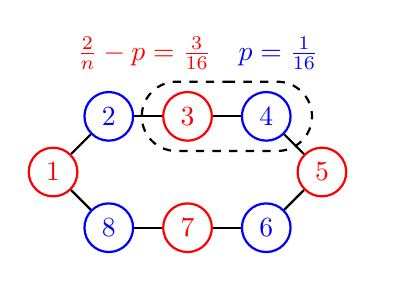
\begin{tikzpicture}[baseline=(current bounding box.north),-,auto,node distance=1cm,
                    thick,main node/.style={circle,draw,font=\sffamily\bfseries}]

  \node[main node,color=red] (1) {$1$};
  \node[main node,color=blue] (2) [above right of=1] {$2$};
  \node[main node,color=red] (3) [right of=2] {$3$};
  \node[main node,color=blue] (4) [right of=3] {$4$};
  \node[main node,color=red] (5) [below right of=4] {$5$};
  \node[main node,color=blue] (6) [below left of=5] {$6$};
  \node[main node,color=red] (7) [left of=6] {$7$};
  \node[main node,color=blue] (8) [left of=7] {$8$};
  

  \path[every node/.style={font=\sffamily}]
  (1) edge (2)
  (2) edge (3)
  (3) edge (4)
  (4) edge (5)
  (5) edge (6)
  (6) edge (7)
  (7) edge (8)
  (8) edge (1);
  
  \node (Box1) [draw,dashed,rounded rectangle,fit=(3) (4)] {};
  
  \node [shift={(-0.4cm,0.8cm)},text width=2cm,color=red] at (3) {$\frac{2}{n}-p=\frac{3}{16}$};
  \node [shift={(0.4cm,0.8cm)},text width=1.5cm,color=blue] at (4) {$p=\frac{1}{16}$};
   
\end{tikzpicture}
\end{center}
\caption{$C_{8}$ with the \textcolor{blue}{blue nodes being ``even'' nodes} started at with probability $\frac{1}{16}$ and the \textcolor{red}{red nodes being ``odd'' nodes} started at with probability $\frac{3}{16}$.}
\end{myfigure}

\begin{lemma}
When $n$ and $m$ are both even, following the ARHP gives the same lower bound as the random Hamiltonian patrol, i.e $V \geq \frac{m}{n}$.
\end{lemma}

\begin{proof}
During any attack interval $I$ which is of even length, then $W(I)$ contains $m'$ ``even'' and $m'$ ``odd'' nodes for a total of $m=2m'$ nodes. Therefore by following the Alternating Random Hamiltonian Patrol, $\pmb{\pi}_{ARHP}$, with probability $p$ at ``even'' nodes and probability $\frac{2}{n}-p$ at ``odd'' nodes. Then

\begin{align*}
&P(\bm{\pi}_{ARHP},[i,I]) \geq \underbrace{\overbrace{p}^{\text{even node}}+\overbrace{\frac{2}{n}-p}^{\text{odd node}}+p+\frac{2}{n}-p+...+p+\frac{2}{n}-p}_{m=2m' \text{ elements}} \\
&=m' p+m'(\frac{2}{n}-p)=\frac{2m'}{n}=\frac{m}{n} \quad \forall i \in N \quad \forall I \subseteq \mathcal{T}
\end{align*}
Hence as it holds for all pure attacks
$$P(\bm{\pi}_{ARHP},\bm{\phi}) \geq \frac{m}{n} \quad \forall \bm{\phi} \in \Phi$$
Hence $V \geq \frac{m}{n}$ .
\end{proof}

If $m$ is odd, say $m=2m'+1$ then in the above we get two possibilities for each node depending on the interval choice either $p+\frac{m-1}{n}$ or $\frac{m+1}{n}-p$. So choosing anything other than $p=\frac{1}{n}$ (which is the Random Hamiltonian Patrol strategy) gives a worse result for the patroller.

While not getting a better lower bound, the ARHP does give some control on how to perform optimally in a Hamiltonian graph. The idea of distributing the probability $\frac{2}{n}$ between two types of nodes can be extended to the idea of distributing the probability $\frac{k}{n}$ between $k$ types of nodes (as seen in Appendix \ref{Appendix:Generalised ARHP}).


We now look at extending the idea of the diametric attack. First we notice that we are not forced to use the graph's diameter, $\bar{d}$, and in fact we can use any distance between two selected nodes, $d$. We replace $\bar{d}$ with $d$ to get a two node distance attack, giving us a bound of $V \leq \max \{\frac{1}{2} ,\frac{m}{2d} \}$. However this cannot be a better bound than using the graph's diameter, so this is not useful.

A useful extension, would be not using two nodes but using multiple points each the same distance apart from each other mutually.

\begin{definition}[Polygonal attack]
A \textit{$d$-polygonal attack} is an attack at a set of nodes $D$ such that $d(i,i')=d \; \forall i,i' \in D$ at the time intervals $I,I+1,...,I+d-1$ (for a chosen initial $I$)
\end{definition}

We can also consider having the points at least the same distance apart

\begin{definition}[Uneven polygonal attack]
A \textit{$d$-uneven polygonal attack} is an attack at a set of nodes $D$ such that $d(i,i') \geq d \; \forall i,i' \in D$ at the time intervals $I,I+1,...,I+d-1$ (for a chosen initial $I$)
\end{definition}

We need to consider the feasibility of these attacks, due to requiring $d$ potential starting times, we need that $T \geq m-d+1$

The idea behind this attack is very similar to the timed-limited diametric attack.

\begin{lemma}
When $T \geq m+d-1$ and a set $D$ as in the $d$- polygonal attack, the bound $V \leq \max \{ \frac{1}{|D|} , \frac{m}{|D|d} \}$ is valid
\end{lemma}

The proof follows the same logic as the time-limited diametric attack, except there are now more points which are each $d$ away.

We conjecture that the uneven-polygonal attack also has the same bound as the polygonal one, as the idea is that any that are strictly greater are just worse for the patroller. However this idea is not yet formalized.


\subsection{Star graph solution}
As a special case of complete bipartite graph we have the star graph, $S_{n}=K_{1,n}$, that is a tree with one internal node (the centre) and $n$ leaf nodes (the external nodes). Hence $V(S_{n})=V(K_{1,n})=\frac{m}{2n}$ for $m<2n$ (by Theorem 15 (1) in \cite{Lin2013}). This is achieved by the patroller forming a patrol which alternates between different  external nodes and the centre, and embedded Hamiltonian patrol from $C_{2n}$, and the attacker attacking at all the external nodes with equal probability for a fixed time interval (or two consecutive time intervals if $m$ is odd).

\subsection{Elongating the star graph}
The line and star graphs provided a good starting point for attempting to solve the problem for a general tree graph. If a more general version of the star graph can be solved, it may provide better bounds on tree graphs. 

The idea is to extend the star graph to a more general graph, which is a mix between the line and the star, by extending the length of the branches (at first just one branch). This may better model a tightly packed region to search and another that is far away, consider the example of a small town and larger city connected by a road. 

\begin{definition}[Elongated Star Graph]
The \textit{Elongated Star Graph}, $S_{n}^{k}$ is made from $S_{n}$, by performing subdivision on one of the edges repeatedly $k$ times, so that one of the external nodes is now $k+1$ away from the centre.
\end{definition}

The labelling will be done as in figure \ref{Figure:Example of elongated labelling}, we note that $*$ nodes are symmetric and so we will be dealing with strategies that treat them as equal (see section 3.1 in \cite{Lin2013}). We will from now assume that $n \geq 3$, as otherwise we are just dealing with the line graph, however we can think of $n=2$ to get the results for the line graph for comparison.


\begin{myfigure}
\begin{center}
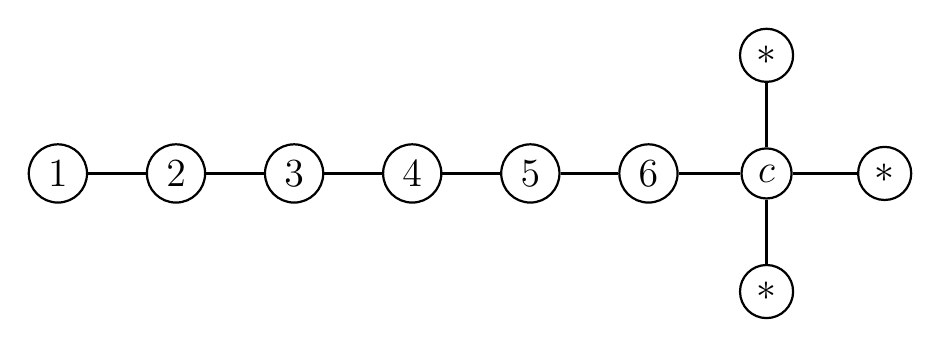
\begin{tikzpicture}[-,auto,node distance=1.5cm,
                    thick,main node/.style={circle,draw,font=\sffamily\Large\bfseries}]

  \node[main node] (1) {$1$};
  \node[main node] (2) [right of=1] {$2$};
  \node[main node] (3) [right of=2] {$3$};
  \node[main node] (4) [right of=3] {$4$};
  \node[main node] (5) [right of=4] {$5$};
  \node[main node] (6) [right of=5]  {$6$};
  \node[main node] (7) [right of=6]  {$c$};
  \node[main node] (8) [right of=7]  {$*$};
  \node[main node] (9) [above of=7]  {$*$};
  \node[main node] (10) [below of=7]  {$*$};
  

  \path[every node/.style={font=\sffamily}]
    (1) edge  (2)
    (2) edge (3)
    (3) edge (4)
    (4) edge (5)
    (5) edge (6)
    (6) edge (7)
    (7) edge (8)
     edge (9)
     edge (10);
\end{tikzpicture}
\end{center}
\caption{Labeling on the graph $S_{4}^5$.}
\label{Figure:Example of elongated labelling}
\end{myfigure}

To start our analysis of this graph, we can look at an expanded graph which can simplify down to our extended star graph. Consider the cyclic graph $C_{(2k+1)+(2n-1)}=C_{2(n+k)}$, we can simplify this graph to $S_{n}^{k}$.


\begin{myfigure}
\begin{center}
\resizebox{\textwidth}{!}{
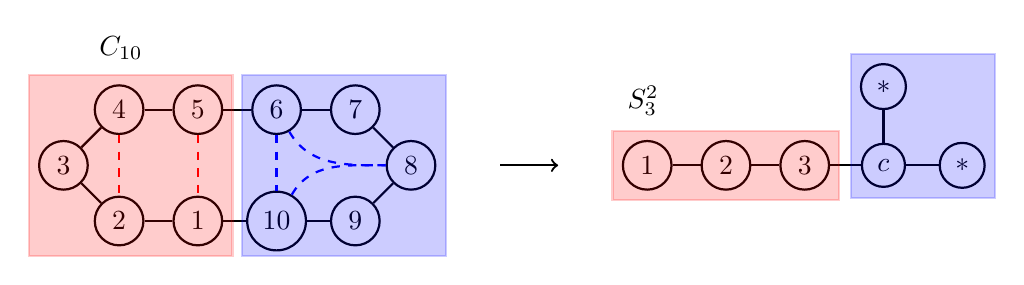
\begin{tikzpicture}[baseline=(current bounding box.north),-,auto,node distance=1cm,
                    thick,main node/.style={circle,draw,font=\sffamily\bfseries}]

  \node[main node] (1) {$3$};
  \node[main node] (2) [above right of=1] {$4$};
  \node[main node] (3) [right of=2] {$5$};
  \node[main node] (4) [right of=3] {$6$};
  \node[main node] (5) [right of=4] {$7$};
  \node[main node] (6) [below right of=5] {$8$};
  \node[main node] (7) [below right of=1] {$2$};
  \node[main node] (8) [right of=7] {$1$};
  \node[main node] (9) [right of=8] {$10$};
  \node[main node] (10) [right of=9] {$9$};
  
  \node (P1) [right of=6] {};
  \node (P2) [right of=P1] {};
  
  \node[main node] (a) [right of=P2] {$1$};
  \node[main node] (b) [right of=a] {$2$};
  \node[main node] (c) [right of=b] {$3$};
  \node[main node] (d) [right of=c] {$c$};
  \node[main node] (e) [right of=d] {$*$};
  \node[main node] (f) [above of=d] {$*$};
  
  \draw[->] (P1) edge (P2);
  

  \path[every node/.style={font=\sffamily}]
    (1) edge  (2)
    edge (7)
    (2) edge (3)
    (3) edge (4)
    (4) edge (5)
    (5) edge (6)
    (6) edge (10)
    (7) edge (8)
    (8) edge (9)
    (9) edge (10)
    (a) edge (b)
    (b) edge (c)
    (c) edge (d)
    (d) edge (e)
    edge (f);
    
     \path[dashed,red,every node/.style={font=\sffamily}]
    (2) edge  (7)
    (3) edge (8);
    
    \path[dashed,blue,every node/.style={font=\sffamily}]
    (4) edge  (9);
    
    \path[dashed,blue,out=-60,in=180,every node/.style={font=\sffamily}]
    (4) edge (6);
    
    \path[dashed,blue,out=60,in=180,every node/.style={font=\sffamily}]
    (9) edge (6);
  
  \node (Box1) [draw,thick,fit=(1) (2) (3) (7) (8),fill,red,opacity=0.2] {};
  \node (Box2) [draw,thick,fit=(4) (5) (6)  (10),fill,blue,opacity=0.2] {};
  
  \node (Box3) [draw,thick,fit=(a) (b) (c),fill,red,opacity=0.2] {}; 
  \node (Box4) [draw,thick,fit=(d) (e) (f),fill,blue,opacity=0.2] {};   
  
\node [left=0.5cm,above=0.5cm,text width=0.5cm] at (2) {$C_{10}$};
\node [left=0.5cm,above=0.5cm,text width=0.5cm] at (a) {$S_{3}^{2}$};   
\end{tikzpicture}
}
\end{center}
\caption{$C_{10}$ can be simplified to $S_{3}^{2}$ by node identifying.}
\end{myfigure}


\begin{definition}[Random Oscillation]
The simplification map from $C_{2(n+k)}$ to $S_{n}^{k}$ is a mapping form nodes $i$ and $2k+2-i$ to node $i$ for $i=1,...,k$ and $2k,2k+2,...,2k+2n-2$ to node $c$ and $2k+2j-1$ to node $*$ for $j=1,...,n-1$.

The \textit{oscillation} on $S_{n}^{k}$ is any embedded Hamiltonian patrol on $C_{2(n+k)}$ under the simplification above.

The \textit{random oscillation} on $S_{n}^{k}$ is the embedded random Hamiltonian patrol on $C_{2(n+k)}$ under the simplification above.
\end{definition}

\begin{lemma}
For $m \leq 2(n+k)$ following the Random Oscillation,
$$V(S_{n}^{k}) \geq \frac{m}{2(n+k)}$$
and if $m > 2(n+k)$ then $V(S_{n}^{k})=1$, achieved by any Oscillation.
\end{lemma}

The proof follows immediately from the simplification bound(Lemma 1 (4) in \cite{Alpern2011}) and the Hamiltonian solution(Theorem 13 (1) in \cite{Alpern2011}) i.e.

\begin{align*}
V(S_{n}^{k}) \geq V(C_{2(n+k)})=\frac{m}{2(n+k)}
\end{align*}

Hence we have the solution in $m > 2(n+k)$ , so we can now restrict ourselves to $m \leq 2(n+k)$.


\begin{note}
We have the solution for $m=2(n+k)$, but to be consistent with the regions in the line graph, we will pull this into the next region.
\end{note}

We could now consider applying the time-limited diametric attack to get bounds on the problem, $\bar{d}=n-1$ gives the bound $V \leq \max \{\frac{1}{2} , \frac{m}{2(n-1)}  \}$, however this bound is not tight with our random oscillation bound, this is because we are not utilising all $*$ type nodes.

Instead of using just one $*$ node (which by symmetry will never yield optimal) we must utilise all the $*$ nodes equally, we can use weights on the distance from the centre. However when using these weights we must spread out  the attack at each position in time, to ensure each potential attack in space and time has an equal weight.

Similiar to the proof of the bipartite graph bounds(Theorem 15 (1) in \cite{Alpern2011}), a timing issue arises when $m$ is odd, however using two fixed time intervals fixes this problem. This holds even when $m$ is even, hence to avoid the problem we will use a baseline spread of two consecutive time periods and then spread out from these according to the weight.

\begin{definition}[Time-delayed attack]
Let the \textit{time-delayed attack}, be the attack that attacks at the extended node labeled $1$ with probability $\frac{k+1}{n+k}$ and a particular normal node labeled $*$ with probability $\frac{1}{n+k}$.

If node $1$ is chosen for the attack, choose time intervals, $I,I+1,...,I+2k+1$, each with equal probability for some fixed time interval, $I$ (i.e starting attacks at $\tau, \tau+1,...,\tau+2k+1$ equiprobably). If a $*$ node is chosen for the attack, choose time intervals, $I+k,I+k+1$, each with equal probability(i.e starting at times $\tau+k,\tau+k+1$ equiprobably).
\end{definition}

A diagram showing how the potential attacks are spaced out in time can be seen in figure \ref{Figure:Time spacing of the time-delayed attack}.

\begin{myfigure}
\begin{center}
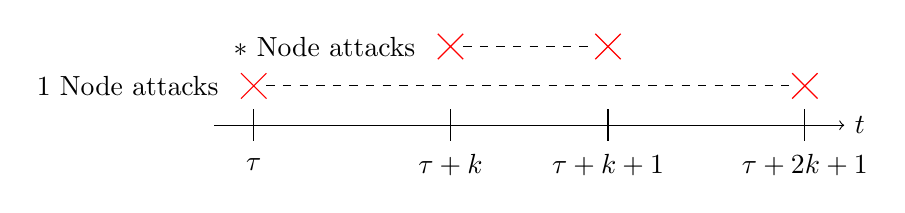
\begin{tikzpicture}
 %Drawing Bottom Axis
 \draw[->] (-4,0) -- (4,0);
 \node (timelabel) [shift={(0.2,0)}] at (4,0) {$t$};
 \draw (-3.5,0.2) -- (-3.5,-0.2);
 \draw (3.5,0.2) -- (3.5,-0.2);
 
 %Drawing Cross and lines 
 \node (labelc1) at (-3.5,-0.5) {$\tau$};
 \node (labelc2) at (3.5,-0.5) {$\tau+2k+1$};
 
 \node[cross=5pt,red] (c1) at (-3.5,0.5) {};
 \node[cross=5pt,red] (c2) at (3.5,0.5) {};
 \draw[dashed] (c1) -- (c2);
 \node (linelabel1) at (-5.1,0.5) {$1$ Node attacks};
 
 
 \draw (-1,0.2) -- (-1,-0.2);
 \draw (1,0.2) -- (1,-0.2);
 
  \node (labelc3) at (-1,-0.5) {$\tau+k$};
 \node (labelc4) at (1,-0.5) {$\tau+k+1$};
 
 \node[cross=5pt,red] (c3) at (-1,1) {};
 \node[cross=5pt,red] (c4) at (1,1) {};
 \draw[dashed] (c3) -- (c4);
 \node (linelabel1) at (-2.6,1) {$*$ Node attacks}; 

\end{tikzpicture}
\end{center}
\caption{Time spacing of the time-delayed attack, for node $1$ and $*$ nodes.}
\label{Figure:Time spacing of the time-delayed attack}
\end{myfigure}

\begin{note}
By making the spread in time proportional to the weight of attacking the node, each potential attack in space and time has the same weight.
\end{note}

\begin{lemma}
When $T \geq m+2k$, the upper bound $V \leq \max \{ \frac{k+1}{n+k} , \frac{m}{2(n+k)}   \}$  is guaranteed by the time-delayed attack.
\end{lemma}

This bound is analogous to the diametric bound, and as long as we are in the range where $m \geq 2(k+1)$ so the lemma gives $V \leq \frac{m}{2(n+k)}$.

\begin{theorem}[Solution in $m \geq 2(k+1)$]
When $T \geq m+2k$, by the attacker using the time-delayed attack and the patroller using a random oscillation patrol, we achieve the value, when $2(k+1) \leq m \leq 2(n+k)$, of
$$V=\frac{m}{2(n+k)}$$
\end{theorem}

Hence we have a solution for 2 regions $m > 2(n+k)$ and $2(k+1) \leq m \leq 2(n+k)$, which we note are analogous to regions $S_{1}$ and $S_{2}$ in the line graph. Hence prompting definitions for our regions

\begin{itemize}
\item $S_{1}' = \{(n,m,k) \, | \, m > 2(n+k) \}$ which have values $V=1$
\item $S_{2}' = \{(n,m,k) \, | \, 2(k+1) \leq m \leq 2(n+k) \}$ which have values $V=\frac{m}{2(n+k)}$
\end{itemize}

An example of these regions and the elongated star graph's value can be seen in \ref{Figure:Elongated star graph region 1 and 2 value}

\begin{myfigure}
\begin{center}
% Created by tikzDevice version 0.10.1 on 2017-11-10 10:35:56
% !TEX encoding = UTF-8 Unicode
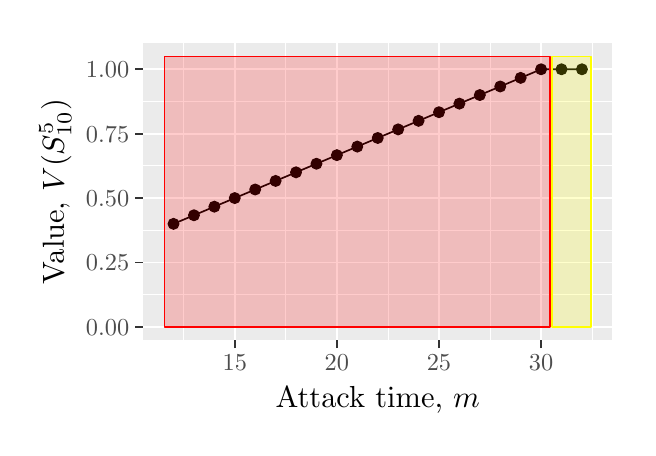
\begin{tikzpicture}[x=1pt,y=1pt]
\definecolor{fillColor}{RGB}{255,255,255}
\path[use as bounding box,fill=fillColor,fill opacity=0.00] (0,0) rectangle (216.81,144.54);
\begin{scope}
\path[clip] (  0.00,  0.00) rectangle (216.81,144.54);
\definecolor{drawColor}{RGB}{255,255,255}
\definecolor{fillColor}{RGB}{255,255,255}

\path[draw=drawColor,line width= 0.6pt,line join=round,line cap=round,fill=fillColor] (  0.00,  0.00) rectangle (216.81,144.54);
\end{scope}
\begin{scope}
\path[clip] ( 41.67, 31.53) rectangle (211.31,139.04);
\definecolor{fillColor}{gray}{0.92}

\path[fill=fillColor] ( 41.67, 31.53) rectangle (211.31,139.04);
\definecolor{drawColor}{RGB}{255,255,255}

\path[draw=drawColor,line width= 0.3pt,line join=round] ( 41.67, 48.05) --
	(211.31, 48.05);

\path[draw=drawColor,line width= 0.3pt,line join=round] ( 41.67, 71.32) --
	(211.31, 71.32);

\path[draw=drawColor,line width= 0.3pt,line join=round] ( 41.67, 94.59) --
	(211.31, 94.59);

\path[draw=drawColor,line width= 0.3pt,line join=round] ( 41.67,117.86) --
	(211.31,117.86);

\path[draw=drawColor,line width= 0.3pt,line join=round] ( 56.39, 31.53) --
	( 56.39,139.04);

\path[draw=drawColor,line width= 0.3pt,line join=round] ( 93.28, 31.53) --
	( 93.28,139.04);

\path[draw=drawColor,line width= 0.3pt,line join=round] (130.18, 31.53) --
	(130.18,139.04);

\path[draw=drawColor,line width= 0.3pt,line join=round] (167.07, 31.53) --
	(167.07,139.04);

\path[draw=drawColor,line width= 0.3pt,line join=round] (203.97, 31.53) --
	(203.97,139.04);

\path[draw=drawColor,line width= 0.6pt,line join=round] ( 41.67, 36.42) --
	(211.31, 36.42);

\path[draw=drawColor,line width= 0.6pt,line join=round] ( 41.67, 59.69) --
	(211.31, 59.69);

\path[draw=drawColor,line width= 0.6pt,line join=round] ( 41.67, 82.96) --
	(211.31, 82.96);

\path[draw=drawColor,line width= 0.6pt,line join=round] ( 41.67,106.23) --
	(211.31,106.23);

\path[draw=drawColor,line width= 0.6pt,line join=round] ( 41.67,129.50) --
	(211.31,129.50);

\path[draw=drawColor,line width= 0.6pt,line join=round] ( 74.83, 31.53) --
	( 74.83,139.04);

\path[draw=drawColor,line width= 0.6pt,line join=round] (111.73, 31.53) --
	(111.73,139.04);

\path[draw=drawColor,line width= 0.6pt,line join=round] (148.63, 31.53) --
	(148.63,139.04);

\path[draw=drawColor,line width= 0.6pt,line join=round] (185.52, 31.53) --
	(185.52,139.04);
\definecolor{drawColor}{RGB}{0,0,0}
\definecolor{fillColor}{RGB}{0,0,0}

\path[draw=drawColor,line width= 0.4pt,line join=round,line cap=round,fill=fillColor] (192.90,129.50) circle (  1.96);

\path[draw=drawColor,line width= 0.4pt,line join=round,line cap=round,fill=fillColor] (200.28,129.50) circle (  1.96);

\path[draw=drawColor,line width= 0.4pt,line join=round,line cap=round,fill=fillColor] ( 52.70, 73.65) circle (  1.96);

\path[draw=drawColor,line width= 0.4pt,line join=round,line cap=round,fill=fillColor] ( 60.08, 76.75) circle (  1.96);

\path[draw=drawColor,line width= 0.4pt,line join=round,line cap=round,fill=fillColor] ( 67.46, 79.86) circle (  1.96);

\path[draw=drawColor,line width= 0.4pt,line join=round,line cap=round,fill=fillColor] ( 74.83, 82.96) circle (  1.96);

\path[draw=drawColor,line width= 0.4pt,line join=round,line cap=round,fill=fillColor] ( 82.21, 86.06) circle (  1.96);

\path[draw=drawColor,line width= 0.4pt,line join=round,line cap=round,fill=fillColor] ( 89.59, 89.16) circle (  1.96);

\path[draw=drawColor,line width= 0.4pt,line join=round,line cap=round,fill=fillColor] ( 96.97, 92.27) circle (  1.96);

\path[draw=drawColor,line width= 0.4pt,line join=round,line cap=round,fill=fillColor] (104.35, 95.37) circle (  1.96);

\path[draw=drawColor,line width= 0.4pt,line join=round,line cap=round,fill=fillColor] (111.73, 98.47) circle (  1.96);

\path[draw=drawColor,line width= 0.4pt,line join=round,line cap=round,fill=fillColor] (119.11,101.57) circle (  1.96);

\path[draw=drawColor,line width= 0.4pt,line join=round,line cap=round,fill=fillColor] (126.49,104.68) circle (  1.96);

\path[draw=drawColor,line width= 0.4pt,line join=round,line cap=round,fill=fillColor] (133.87,107.78) circle (  1.96);

\path[draw=drawColor,line width= 0.4pt,line join=round,line cap=round,fill=fillColor] (141.25,110.88) circle (  1.96);

\path[draw=drawColor,line width= 0.4pt,line join=round,line cap=round,fill=fillColor] (148.63,113.99) circle (  1.96);

\path[draw=drawColor,line width= 0.4pt,line join=round,line cap=round,fill=fillColor] (156.00,117.09) circle (  1.96);

\path[draw=drawColor,line width= 0.4pt,line join=round,line cap=round,fill=fillColor] (163.38,120.19) circle (  1.96);

\path[draw=drawColor,line width= 0.4pt,line join=round,line cap=round,fill=fillColor] (170.76,123.29) circle (  1.96);

\path[draw=drawColor,line width= 0.4pt,line join=round,line cap=round,fill=fillColor] (178.14,126.40) circle (  1.96);

\path[draw=drawColor,line width= 0.4pt,line join=round,line cap=round,fill=fillColor] (185.52,129.50) circle (  1.96);

\path[draw=drawColor,line width= 0.6pt,line join=round] ( 52.70, 73.65) --
	( 60.08, 76.75) --
	( 67.46, 79.86) --
	( 74.83, 82.96) --
	( 82.21, 86.06) --
	( 89.59, 89.16) --
	( 96.97, 92.27) --
	(104.35, 95.37) --
	(111.73, 98.47) --
	(119.11,101.57) --
	(126.49,104.68) --
	(133.87,107.78) --
	(141.25,110.88) --
	(148.63,113.99) --
	(156.00,117.09) --
	(163.38,120.19) --
	(170.76,123.29) --
	(178.14,126.40) --
	(185.52,129.50) --
	(192.90,129.50) --
	(200.28,129.50);
\definecolor{drawColor}{RGB}{255,255,0}
\definecolor{fillColor}{RGB}{255,255,0}

\path[draw=drawColor,line width= 0.6pt,line join=round,fill=fillColor,fill opacity=0.20] (189.58, 36.42) rectangle (203.60,134.15);
\definecolor{drawColor}{RGB}{255,0,0}
\definecolor{fillColor}{RGB}{255,0,0}

\path[draw=drawColor,line width= 0.6pt,line join=round,fill=fillColor,fill opacity=0.20] ( 49.38, 36.42) rectangle (188.84,134.15);
\end{scope}
\begin{scope}
\path[clip] (  0.00,  0.00) rectangle (216.81,144.54);
\definecolor{drawColor}{gray}{0.30}

\node[text=drawColor,anchor=base east,inner sep=0pt, outer sep=0pt, scale=  0.88] at ( 36.72, 33.39) {0.00};

\node[text=drawColor,anchor=base east,inner sep=0pt, outer sep=0pt, scale=  0.88] at ( 36.72, 56.66) {0.25};

\node[text=drawColor,anchor=base east,inner sep=0pt, outer sep=0pt, scale=  0.88] at ( 36.72, 79.93) {0.50};

\node[text=drawColor,anchor=base east,inner sep=0pt, outer sep=0pt, scale=  0.88] at ( 36.72,103.20) {0.75};

\node[text=drawColor,anchor=base east,inner sep=0pt, outer sep=0pt, scale=  0.88] at ( 36.72,126.47) {1.00};
\end{scope}
\begin{scope}
\path[clip] (  0.00,  0.00) rectangle (216.81,144.54);
\definecolor{drawColor}{gray}{0.20}

\path[draw=drawColor,line width= 0.6pt,line join=round] ( 38.92, 36.42) --
	( 41.67, 36.42);

\path[draw=drawColor,line width= 0.6pt,line join=round] ( 38.92, 59.69) --
	( 41.67, 59.69);

\path[draw=drawColor,line width= 0.6pt,line join=round] ( 38.92, 82.96) --
	( 41.67, 82.96);

\path[draw=drawColor,line width= 0.6pt,line join=round] ( 38.92,106.23) --
	( 41.67,106.23);

\path[draw=drawColor,line width= 0.6pt,line join=round] ( 38.92,129.50) --
	( 41.67,129.50);
\end{scope}
\begin{scope}
\path[clip] (  0.00,  0.00) rectangle (216.81,144.54);
\definecolor{drawColor}{gray}{0.20}

\path[draw=drawColor,line width= 0.6pt,line join=round] ( 74.83, 28.78) --
	( 74.83, 31.53);

\path[draw=drawColor,line width= 0.6pt,line join=round] (111.73, 28.78) --
	(111.73, 31.53);

\path[draw=drawColor,line width= 0.6pt,line join=round] (148.63, 28.78) --
	(148.63, 31.53);

\path[draw=drawColor,line width= 0.6pt,line join=round] (185.52, 28.78) --
	(185.52, 31.53);
\end{scope}
\begin{scope}
\path[clip] (  0.00,  0.00) rectangle (216.81,144.54);
\definecolor{drawColor}{gray}{0.30}

\node[text=drawColor,anchor=base,inner sep=0pt, outer sep=0pt, scale=  0.88] at ( 74.83, 20.52) {15};

\node[text=drawColor,anchor=base,inner sep=0pt, outer sep=0pt, scale=  0.88] at (111.73, 20.52) {20};

\node[text=drawColor,anchor=base,inner sep=0pt, outer sep=0pt, scale=  0.88] at (148.63, 20.52) {25};

\node[text=drawColor,anchor=base,inner sep=0pt, outer sep=0pt, scale=  0.88] at (185.52, 20.52) {30};
\end{scope}
\begin{scope}
\path[clip] (  0.00,  0.00) rectangle (216.81,144.54);
\definecolor{drawColor}{RGB}{0,0,0}

\node[text=drawColor,anchor=base,inner sep=0pt, outer sep=0pt, scale=  1.10] at (126.49,  7.44) {Attack time, $m$};
\end{scope}
\begin{scope}
\path[clip] (  0.00,  0.00) rectangle (216.81,144.54);
\definecolor{drawColor}{RGB}{0,0,0}

\node[text=drawColor,rotate= 90.00,anchor=base,inner sep=0pt, outer sep=0pt, scale=  1.10] at ( 13.08, 85.29) {Value, $V(S_{ 10 }^{ 5 })$};
\end{scope}
\end{tikzpicture}

\end{center}
\caption{Value of the elongated star graph, $S_{10}^{5}$}
\label{Figure:Elongated star graph region 1 and 2 value}
\end{myfigure}

We then seek solutions in the region $m < 2(k+1)$, however in this region we are below the random oscillation bound for the patroller and we can suggest some improvement (as in $S_{5}$ in the line graph) from the embedded Hamiltonian bound with. To see the issue and why the random oscillation can be improved we will look at the probability of interception under this patrol strategy.

If the patroller is performing a random oscillation, then for a pure attack at node $i$ the probability of capture is given by (derivation in appendix \ref{Appendix:Reason for probability of interception}),
\begin{equation}
\label{eq:Prob of Interception}
w(i)= \left\{\begin{array}{l}
 \frac{\min(m+2(i-1),2m)}{2(n+k)} \text{  , for } i \leq \frac{n+k}{2} +1, \\
 \frac{\min(m+2(n+k+1-i),2m)}{2(n+k)} \text{  , for } i > \frac{n+k}{2} +1, \\
 \frac{\min(m+2(n-1),nm)}{2(n+k)} \text{  , for } i=c, \\
 \frac{m}{2(n+k)} \text{  , for } i=*. 
\end{array} \right.
\end{equation}
We will call $w(i)$ the probability of \textit{interception} at node $i$.

\begin{myfigure}
\begin{center}
% Created by tikzDevice version 0.10.1 on 2017-11-24 11:28:25
% !TEX encoding = UTF-8 Unicode
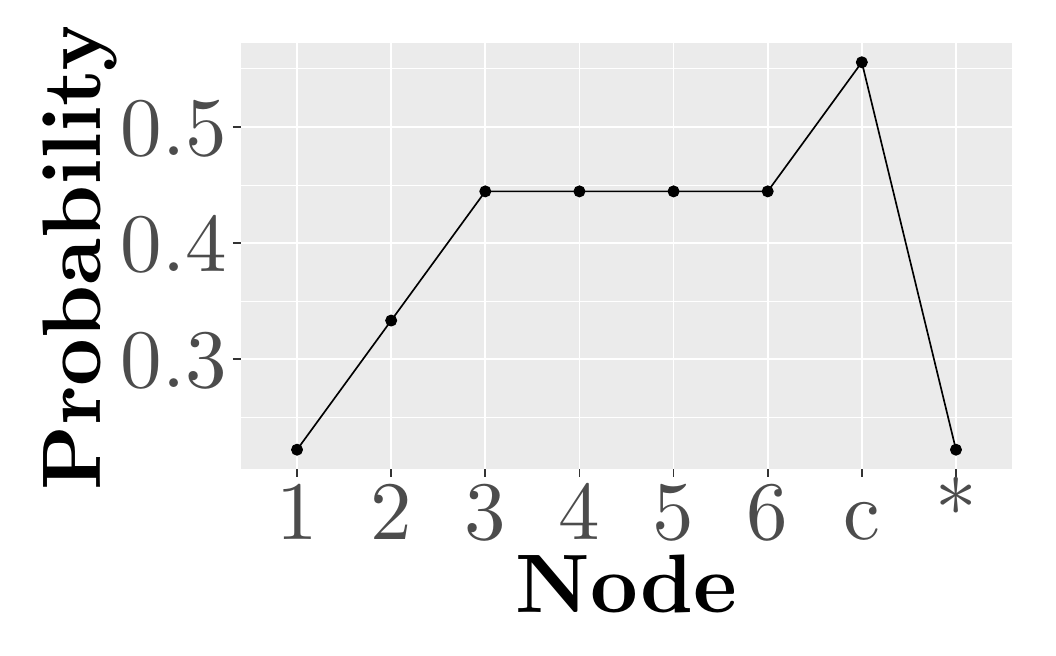
\begin{tikzpicture}[x=1pt,y=1pt]
\definecolor{fillColor}{RGB}{255,255,255}
\path[use as bounding box,fill=fillColor,fill opacity=0.00] (0,0) rectangle (361.35,216.81);
\begin{scope}
\path[clip] (  0.00,  0.00) rectangle (361.35,216.81);
\definecolor{drawColor}{RGB}{255,255,255}
\definecolor{fillColor}{RGB}{255,255,255}

\path[draw=drawColor,line width= 0.6pt,line join=round,line cap=round,fill=fillColor] (  0.00,  0.00) rectangle (361.35,216.81);
\end{scope}
\begin{scope}
\path[clip] ( 76.92, 57.31) rectangle (355.85,211.31);
\definecolor{fillColor}{gray}{0.92}

\path[fill=fillColor] ( 76.92, 57.31) rectangle (355.85,211.31);
\definecolor{drawColor}{RGB}{255,255,255}

\path[draw=drawColor,line width= 0.3pt,line join=round] ( 76.92, 75.98) --
	(355.85, 75.98);

\path[draw=drawColor,line width= 0.3pt,line join=round] ( 76.92,117.98) --
	(355.85,117.98);

\path[draw=drawColor,line width= 0.3pt,line join=round] ( 76.92,159.98) --
	(355.85,159.98);

\path[draw=drawColor,line width= 0.3pt,line join=round] ( 76.92,201.98) --
	(355.85,201.98);

\path[draw=drawColor,line width= 0.6pt,line join=round] ( 76.92, 96.98) --
	(355.85, 96.98);

\path[draw=drawColor,line width= 0.6pt,line join=round] ( 76.92,138.98) --
	(355.85,138.98);

\path[draw=drawColor,line width= 0.6pt,line join=round] ( 76.92,180.98) --
	(355.85,180.98);

\path[draw=drawColor,line width= 0.6pt,line join=round] ( 97.33, 57.31) --
	( 97.33,211.31);

\path[draw=drawColor,line width= 0.6pt,line join=round] (131.35, 57.31) --
	(131.35,211.31);

\path[draw=drawColor,line width= 0.6pt,line join=round] (165.36, 57.31) --
	(165.36,211.31);

\path[draw=drawColor,line width= 0.6pt,line join=round] (199.38, 57.31) --
	(199.38,211.31);

\path[draw=drawColor,line width= 0.6pt,line join=round] (233.39, 57.31) --
	(233.39,211.31);

\path[draw=drawColor,line width= 0.6pt,line join=round] (267.41, 57.31) --
	(267.41,211.31);

\path[draw=drawColor,line width= 0.6pt,line join=round] (301.42, 57.31) --
	(301.42,211.31);

\path[draw=drawColor,line width= 0.6pt,line join=round] (335.44, 57.31) --
	(335.44,211.31);
\definecolor{drawColor}{RGB}{0,0,0}
\definecolor{fillColor}{RGB}{0,0,0}

\path[draw=drawColor,line width= 0.4pt,line join=round,line cap=round,fill=fillColor] ( 97.33, 64.31) circle (  1.96);

\path[draw=drawColor,line width= 0.4pt,line join=round,line cap=round,fill=fillColor] (131.35,110.98) circle (  1.96);

\path[draw=drawColor,line width= 0.4pt,line join=round,line cap=round,fill=fillColor] (165.36,157.65) circle (  1.96);

\path[draw=drawColor,line width= 0.4pt,line join=round,line cap=round,fill=fillColor] (199.38,157.65) circle (  1.96);

\path[draw=drawColor,line width= 0.4pt,line join=round,line cap=round,fill=fillColor] (233.39,157.65) circle (  1.96);

\path[draw=drawColor,line width= 0.4pt,line join=round,line cap=round,fill=fillColor] (267.41,157.65) circle (  1.96);

\path[draw=drawColor,line width= 0.4pt,line join=round,line cap=round,fill=fillColor] (301.42,204.31) circle (  1.96);

\path[draw=drawColor,line width= 0.4pt,line join=round,line cap=round,fill=fillColor] (335.44, 64.31) circle (  1.96);

\path[draw=drawColor,line width= 0.6pt,line join=round] ( 97.33, 64.31) --
	(131.35,110.98) --
	(165.36,157.65) --
	(199.38,157.65) --
	(233.39,157.65) --
	(267.41,157.65) --
	(301.42,204.31) --
	(335.44, 64.31);
\end{scope}
\begin{scope}
\path[clip] (  0.00,  0.00) rectangle (361.35,216.81);
\definecolor{drawColor}{gray}{0.30}

\node[text=drawColor,anchor=base east,inner sep=0pt, outer sep=0pt, scale=  3.00] at ( 71.97, 86.65) {0.3};

\node[text=drawColor,anchor=base east,inner sep=0pt, outer sep=0pt, scale=  3.00] at ( 71.97,128.65) {0.4};

\node[text=drawColor,anchor=base east,inner sep=0pt, outer sep=0pt, scale=  3.00] at ( 71.97,170.65) {0.5};
\end{scope}
\begin{scope}
\path[clip] (  0.00,  0.00) rectangle (361.35,216.81);
\definecolor{drawColor}{gray}{0.20}

\path[draw=drawColor,line width= 0.6pt,line join=round] ( 74.17, 96.98) --
	( 76.92, 96.98);

\path[draw=drawColor,line width= 0.6pt,line join=round] ( 74.17,138.98) --
	( 76.92,138.98);

\path[draw=drawColor,line width= 0.6pt,line join=round] ( 74.17,180.98) --
	( 76.92,180.98);
\end{scope}
\begin{scope}
\path[clip] (  0.00,  0.00) rectangle (361.35,216.81);
\definecolor{drawColor}{gray}{0.20}

\path[draw=drawColor,line width= 0.6pt,line join=round] ( 97.33, 54.56) --
	( 97.33, 57.31);

\path[draw=drawColor,line width= 0.6pt,line join=round] (131.35, 54.56) --
	(131.35, 57.31);

\path[draw=drawColor,line width= 0.6pt,line join=round] (165.36, 54.56) --
	(165.36, 57.31);

\path[draw=drawColor,line width= 0.6pt,line join=round] (199.38, 54.56) --
	(199.38, 57.31);

\path[draw=drawColor,line width= 0.6pt,line join=round] (233.39, 54.56) --
	(233.39, 57.31);

\path[draw=drawColor,line width= 0.6pt,line join=round] (267.41, 54.56) --
	(267.41, 57.31);

\path[draw=drawColor,line width= 0.6pt,line join=round] (301.42, 54.56) --
	(301.42, 57.31);

\path[draw=drawColor,line width= 0.6pt,line join=round] (335.44, 54.56) --
	(335.44, 57.31);
\end{scope}
\begin{scope}
\path[clip] (  0.00,  0.00) rectangle (361.35,216.81);
\definecolor{drawColor}{gray}{0.30}

\node[text=drawColor,anchor=base,inner sep=0pt, outer sep=0pt, scale=  3.00] at ( 97.33, 31.70) {1};

\node[text=drawColor,anchor=base,inner sep=0pt, outer sep=0pt, scale=  3.00] at (131.35, 31.70) {2};

\node[text=drawColor,anchor=base,inner sep=0pt, outer sep=0pt, scale=  3.00] at (165.36, 31.70) {3};

\node[text=drawColor,anchor=base,inner sep=0pt, outer sep=0pt, scale=  3.00] at (199.38, 31.70) {4};

\node[text=drawColor,anchor=base,inner sep=0pt, outer sep=0pt, scale=  3.00] at (233.39, 31.70) {5};

\node[text=drawColor,anchor=base,inner sep=0pt, outer sep=0pt, scale=  3.00] at (267.41, 31.70) {6};

\node[text=drawColor,anchor=base,inner sep=0pt, outer sep=0pt, scale=  3.00] at (301.42, 31.70) {c};

\node[text=drawColor,anchor=base,inner sep=0pt, outer sep=0pt, scale=  3.00] at (335.44, 31.70) {*};
\end{scope}
\begin{scope}
\path[clip] (  0.00,  0.00) rectangle (361.35,216.81);
\definecolor{drawColor}{RGB}{0,0,0}

\node[text=drawColor,anchor=base,inner sep=0pt, outer sep=0pt, scale=  3.00] at (216.39,  5.50) {\bfseries Node};
\end{scope}
\begin{scope}
\path[clip] (  0.00,  0.00) rectangle (361.35,216.81);
\definecolor{drawColor}{RGB}{0,0,0}

\node[text=drawColor,rotate= 90.00,anchor=base,inner sep=0pt, outer sep=0pt, scale=  3.00] at ( 26.20,134.31) {\bfseries Probability};
\end{scope}
\end{tikzpicture}

\end{center}
\caption{Interception probabilities of $S^5_{4}$ when $m=4$.}
\label{Figure:Base interception probabilities}
\end{myfigure}

Looking at the function (or the figure \ref{Figure:Base interception probabilities})it is clear that the issues are towards the end of the graph. This is because the next return under the random oscillation does not provide adequate coverage, hence we may wish to improve these end points of the graph. To do so we introduce the concepts of cycles which are played to guarantee capture of all attacks at all nodes within their cycle(\textit{covering}).

\begin{definition}[End-covering cycle]
Define a cycle of length $m$ (if even) or $m-1$ (if odd) to be \textit{end-covering} if one of the points along the cycle is a leaf node. Define the \textit{half-length} of such cycles to be $\hat{m}=\floor{\frac{m}{2}}$.
\end{definition}

In \cite{Papadaki2016} the authors improved the line graph's end nodes, which have poor interception probabilities, by introducing a end-covering cycle at each end. We shall do the same, though now more consideration needs to be taken on how to place these end-covering cycles. 

We first classify nodes into types, we partition the node set, $N=L \cup M \cup R \cup S$, where
\begin{itemize}
\item Left nodes, $L=\left\{ i \, | \, i \leq \floor{\frac{m}{2}}+1 , i \leq k+1 \right\}$ 
\item Middle nodes, $M=\left\{ i \, | \, \floor{\frac{m}{2}}+2 \leq i \leq n+k-\floor{\frac{m}{2}} , i \leq k+1 \right\}$
\item Right nodes, $R=\left\{ i \, | \, i \geq n+k+1-\floor{\frac{m}{2}} , i \leq k+1 \right\}$
\item Star node, $S=\{ c,* \}$
\end{itemize}

\begin{note}
The set $R$ is empty if $\hat{m} \leq n-1$. The set $M$ is empty if $\hat{m} \geq k-1$ or $\hat{m} \geq n+k-2$.
\end{note}

Then $ V \geq w_{\min} \equiv w_{\min}^{N}=\min \left\{ w_{\min}^{L},w_{\min}^{M},w_{\min}^{R},w_{\min}^{S} \right\}$ , where $w_{\min}^{X}=\min\limits_{i \in X} w(i)$. We aim to use end-ensuring cycles to improve $w_{\min}$, which means improving the worst node sets, and hence improving the random oscillation bound.


Now from equation \ref{eq:Prob of Interception} we note some properties for each node set.
\begin{itemize}
\item $w_{min}^{L}=w(1)$, as for $i \in L$ we have that $w(i)$ is increasing in $i$.
\item $w_{min}^{M}=w(\hat{m}+2)=\frac{2m}{2(n+k)}$ , as for $i \in M $ we have that $w(i)=\frac{2m}{2(n+k)}$ $\forall i \in M$.
\item $w_{min}^{R}=w(k+1)$, as for $i \in R$ we have that $w(i)$ is decreasing in $i$.
\item $w_{min}^{S}=w(*)$, as $w(c) > w(*)$.
\end{itemize}

So as long as the improvement made on $L$ and $M$ is non-decreasing then only the nodes $1$ and $\hat{m}+2$ need be considered. Similarly if in $R$, the improvement is non-increasing then we only need to consider the node $k+1$.Finally if in $S$, the improvement improves node $c$ as good as $*$ then we only need to consider $*$. We shall only consider improving strategies of the type above so only nodes, $1,\hat{m}+2,k+1,*$(if the set is non-empty) need to be considered.

Similarly let $C_{\min}^{X} (\bm{\pi}) = \min\limits_{i \in X} P(\bm{\pi},i)$, where $P(\bm{\pi},i)=\max\limits_{ I \subset \mathcal{T}} P(\bm{\pi},[i,I])$, is the probability of capture under $\bm{\pi}$ and $C_{\min} (\bm{\pi}) \equiv C_{\min}^{N} = \min \left\{ C_{\min}^{L},  C_{\min}^{M},  C_{\min}^{R},  C_{\min}^{S} \right\}$. Then we seek to select $\bm{\pi}$ to get $C_{\min} (\bm{\pi}) > W_{\min} \equiv C_{\min}(\bm{\pi}_{0})$ , where $\bm{\pi}_{0}$ is the random oscillation strategy.

We will use $P$ to be the probability that the random oscillation is played, and $Q=1-P$, to be the probability the improvement is played. We split, $Q$ into $Q=Q_{L}+Q_{M}+Q_{R}+Q_{S}$, where $Q_{X}$ is the amount of probability used to improve the probability of intersection for the set $X$. We use $q_{X}$ to be probability that the minimum of the set is improved by, so $C_{\min}^{X}=PW_{\min}^{X}+q_{X}$.

Multiple choices for possible improvement exist, we first present the most simplest, but naive improvement. The improvement will begin by imagining the $*$ nodes are the ends of $n-1$ lines and improve as in the improvment to the line's hamiltonian bound(section 5 in \cite{Papadaki2016}). Because this approach is naive and is not fully utilising our graphical structure, we will adopt a combinatorial approach to which nodes to improve.

\textbf{A naive improvement}
Let $\bm{\pi}=\bm{\pi}_{N}(Q_{L},Q_{S})$ denote the naive improvement policy. We will play the end-ensuring cycle, $\{1,...,\hat{m}+1,...,1\}$, with probability $Q_{L}$ (a non-decreasing improvement), giving $q_{L}=Q_{L}$. We will play an end-covering cycle for each $*$ node, $\{*,c,....,k+3-\hat{m},....,c,* \}$,(a non-decreasing improvement) with total probability $Q_{S}$, giving $q_{S}=\frac{Q_{S}}{n-1}$.
 
Now we may also have improved some of the nodes in $R$, possibly up to node $k+3-\hat{m} \leq n+k+1-\hat{m}$ (as $n \geq 3$), meaning that all nodes in $R$ are in the end-covering cycle,   $\{*,c,...,k+3-\floor{\frac{m}{2}} \}$ , so the improvement is non-increasing, so $q_{R}=q_{S}$. If $M \neq \emptyset$ nodes in $M$ may be improved, but the node $\hat{m} +2$ will not be improved as  $\hat{m} +2 > \hat{m} +1$ and $\hat{m} +2 < k+3- \hat{m}$ (as $\hat{m} < k-1$ when $M \neq \emptyset$), so the improvement is non-decreasing and $q_{M}=0$.


\begin{examplefigure}
\begin{center}
\resizebox{\textwidth}{!}{
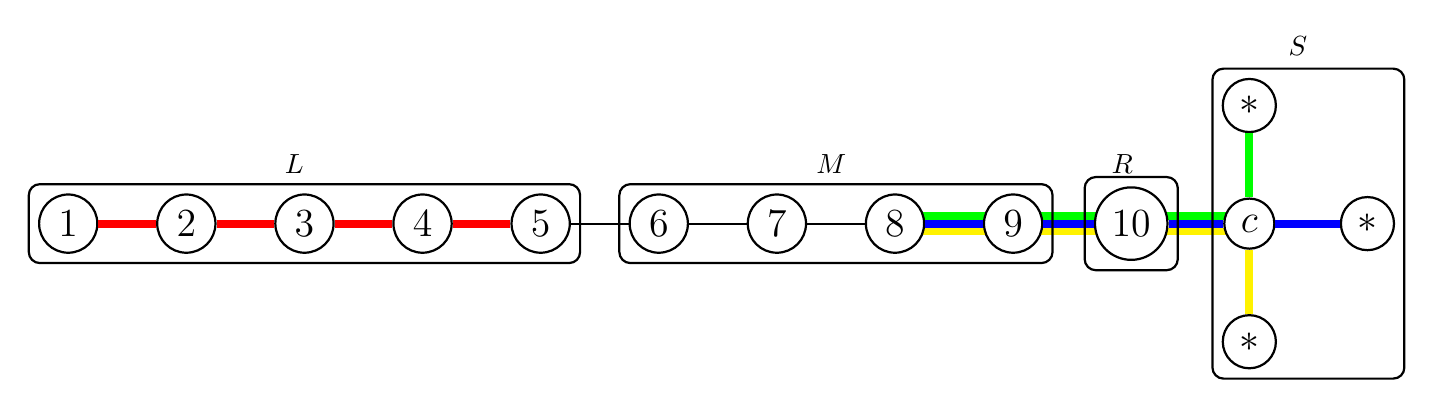
\begin{tikzpicture}[-,auto,node distance=1.5cm,
                    thick,main node/.style={circle,fill=white,draw,font=\sffamily\Large\bfseries}]

  \node[main node] (1) {$1$};
  \node[main node] (2) [right of=1] {$2$};
  \node[main node] (3) [right of=2] {$3$};
  \node[main node] (4) [right of=3] {$4$};
  \node[main node] (5) [right of=4] {$5$};
  \node[main node] (6) [right of=5]  {$6$};
  \node[main node] (7) [right of=6] {$7$};
  \node[main node] (8) [right of=7] {$8$};
  \node[main node] (9) [right of=8] {$9$};
  \node[main node] (10) [right of=9]  {$10$};
  \node[main node] (11) [right of=10]  {$c$};
  \node[main node] (12) [right of=11]  {$*$};
  \node[main node] (13) [above of=11]  {$*$};
  \node[main node] (14) [below of=11]  {$*$};
  

  \path[every node/.style={font=\sffamily}]
    (1) edge  (2)
    (2) edge (3)
    (3) edge (4)
    (4) edge (5)
    (5) edge (6)
    (6) edge (7)
    (7) edge (8)
    (8) edge (9)
    (9) edge (10)
    (10) edge (11)
    (11) edge (12)
    edge (13)
    edge (14);
      
     
   \draw[line width=1mm,color=red] (1) to (2) to (3) to (4) to (5);
   
   \draw [line width=1mm,color=blue] (11) to (12);
   \draw [line width=1mm,color=green] (11) to (13);
   \draw [line width=1mm,color=yellow] (11) to (14);
   \draw [line width=1mm,color=blue] (8) to (9) to (10) to (11);
   
   \node (LBox) [draw,rounded corners, fit= (1) (2) (3) (4) (5)] {};
   \node (MBox) [draw,rounded corners, fit= (6) (7) (8) (9)] {};
   \node (RBox) [draw,rounded corners, fit= (10)] {};
   \node (SBox) [draw,rounded corners, fit= (11) (12) (13) (14)] {};
   
   \node [above=0.5cm,text width=0.5cm] at (LBox) {$L$};
   \node [above=0.5cm,text width=0.5cm] at (MBox) {$M$};
   \node [above=0.5cm,text width=0.5cm] at (RBox) {$R$};
   \node [,above=2cm,text width=0.5cm] at (SBox) {$S$}; 
   
\begin{scope}[on background layer]
   \node[style={circle,,font=\sffamily\Large\bfseries}] (8H) at ($ (8) + (0,0.1) $) { };
   \node[style={circle,,font=\sffamily\Large\bfseries}] (9H) at ($ (9) + (0,0.1) $) { };   
   \node[style={circle,,font=\sffamily\Large\bfseries}] (10H) at ($ (10) + (0,0.1) $) { };
   \node[style={circle,,font=\sffamily\Large\bfseries}] (11H) at ($ (11) + (0,0.1) $) { };
   \draw [line width=1mm,color=green] (8H) to (9H) to (10H) to (11H);
   \node[style={circle,,font=\sffamily\Large\bfseries}] (8L) at ($ (8) + (0,-0.1) $) { };
   \node[style={circle,,font=\sffamily\Large\bfseries}] (9L) at ($ (9) + (0,-0.1) $) { };
   \node[style={circle,,font=\sffamily\Large\bfseries}] (10L) at ($ (10) + (0,-0.1) $) { };
   \node[style={circle,,font=\sffamily\Large\bfseries}] (11L) at ($ (11) + (0,-0.1) $) { };
   \draw [line width=1mm,color=yellow] (8L) to (9L) to (10L) to (11L);
\end{scope}
    
   
\end{tikzpicture}
}
\end{center}
\caption{The Naive Improvement on $S_{4}^{9}$ for $m=9$. The \textcolor{red}{red lines indicating the end-covering cycle $\{1,2,3,4,5,4,3,2,1 \}$} and the other coloured lines indicating the end-ensuring cycles, for each $*$, $\{*,c,10,9,8,9,10,c,* \}$ (as $\hat{m}=4$).}
\end{examplefigure}


Using the Naive Improvement Policy we can achieve an improvement over the random oscillation if $2(n+k) -nm \geq 0$ and get a bound of $V \geq \frac{2m}{2(n+k)+nm}$ (or $V \geq \frac{1}{n}$ if $M=\emptyset,R=\emptyset$), by choosing optimal $Q_{L}$ and $Q_{S}$ (See appendix \ref{Appendix:Naive improvement analysis} for the details).


\begin{myfigure}
\begin{center}
% Created by tikzDevice version 0.10.1 on 2017-11-24 11:28:26
% !TEX encoding = UTF-8 Unicode
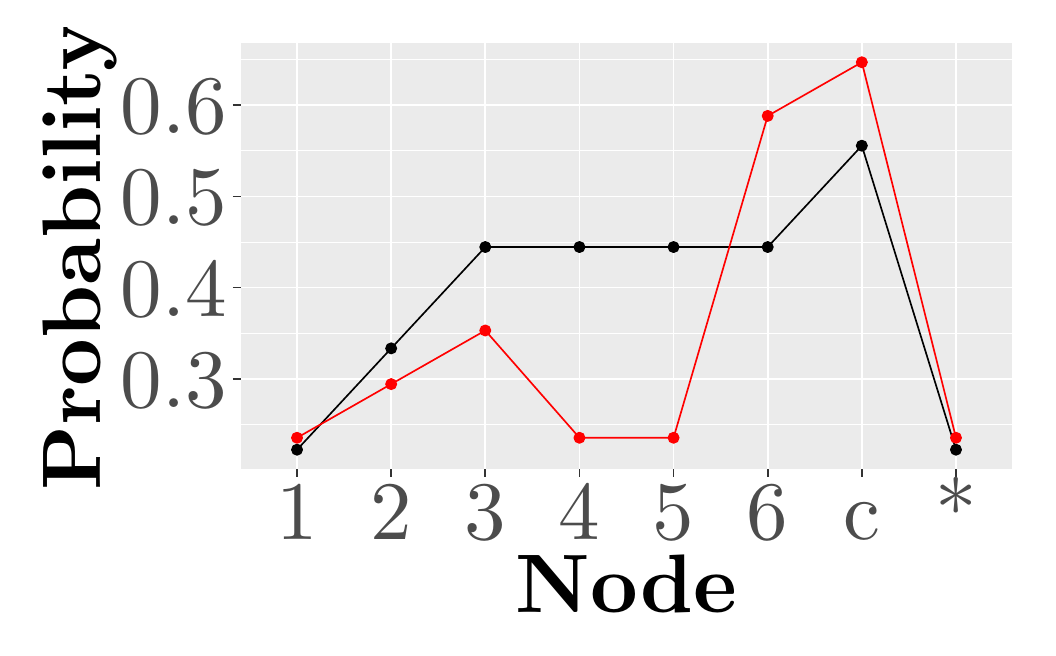
\begin{tikzpicture}[x=1pt,y=1pt]
\definecolor{fillColor}{RGB}{255,255,255}
\path[use as bounding box,fill=fillColor,fill opacity=0.00] (0,0) rectangle (361.35,216.81);
\begin{scope}
\path[clip] (  0.00,  0.00) rectangle (361.35,216.81);
\definecolor{drawColor}{RGB}{255,255,255}
\definecolor{fillColor}{RGB}{255,255,255}

\path[draw=drawColor,line width= 0.6pt,line join=round,line cap=round,fill=fillColor] (  0.00,  0.00) rectangle (361.35,216.81);
\end{scope}
\begin{scope}
\path[clip] ( 76.92, 57.31) rectangle (355.85,211.31);
\definecolor{fillColor}{gray}{0.92}

\path[fill=fillColor] ( 76.92, 57.31) rectangle (355.85,211.31);
\definecolor{drawColor}{RGB}{255,255,255}

\path[draw=drawColor,line width= 0.3pt,line join=round] ( 76.92, 73.47) --
	(355.85, 73.47);

\path[draw=drawColor,line width= 0.3pt,line join=round] ( 76.92,106.42) --
	(355.85,106.42);

\path[draw=drawColor,line width= 0.3pt,line join=round] ( 76.92,139.37) --
	(355.85,139.37);

\path[draw=drawColor,line width= 0.3pt,line join=round] ( 76.92,172.33) --
	(355.85,172.33);

\path[draw=drawColor,line width= 0.3pt,line join=round] ( 76.92,205.28) --
	(355.85,205.28);

\path[draw=drawColor,line width= 0.6pt,line join=round] ( 76.92, 89.94) --
	(355.85, 89.94);

\path[draw=drawColor,line width= 0.6pt,line join=round] ( 76.92,122.90) --
	(355.85,122.90);

\path[draw=drawColor,line width= 0.6pt,line join=round] ( 76.92,155.85) --
	(355.85,155.85);

\path[draw=drawColor,line width= 0.6pt,line join=round] ( 76.92,188.80) --
	(355.85,188.80);

\path[draw=drawColor,line width= 0.6pt,line join=round] ( 97.33, 57.31) --
	( 97.33,211.31);

\path[draw=drawColor,line width= 0.6pt,line join=round] (131.35, 57.31) --
	(131.35,211.31);

\path[draw=drawColor,line width= 0.6pt,line join=round] (165.36, 57.31) --
	(165.36,211.31);

\path[draw=drawColor,line width= 0.6pt,line join=round] (199.38, 57.31) --
	(199.38,211.31);

\path[draw=drawColor,line width= 0.6pt,line join=round] (233.39, 57.31) --
	(233.39,211.31);

\path[draw=drawColor,line width= 0.6pt,line join=round] (267.41, 57.31) --
	(267.41,211.31);

\path[draw=drawColor,line width= 0.6pt,line join=round] (301.42, 57.31) --
	(301.42,211.31);

\path[draw=drawColor,line width= 0.6pt,line join=round] (335.44, 57.31) --
	(335.44,211.31);
\definecolor{drawColor}{RGB}{0,0,0}
\definecolor{fillColor}{RGB}{0,0,0}

\path[draw=drawColor,line width= 0.4pt,line join=round,line cap=round,fill=fillColor] ( 97.33, 64.31) circle (  1.96);

\path[draw=drawColor,line width= 0.4pt,line join=round,line cap=round,fill=fillColor] (131.35,100.93) circle (  1.96);

\path[draw=drawColor,line width= 0.4pt,line join=round,line cap=round,fill=fillColor] (165.36,137.54) circle (  1.96);

\path[draw=drawColor,line width= 0.4pt,line join=round,line cap=round,fill=fillColor] (199.38,137.54) circle (  1.96);

\path[draw=drawColor,line width= 0.4pt,line join=round,line cap=round,fill=fillColor] (233.39,137.54) circle (  1.96);

\path[draw=drawColor,line width= 0.4pt,line join=round,line cap=round,fill=fillColor] (267.41,137.54) circle (  1.96);

\path[draw=drawColor,line width= 0.4pt,line join=round,line cap=round,fill=fillColor] (301.42,174.16) circle (  1.96);

\path[draw=drawColor,line width= 0.4pt,line join=round,line cap=round,fill=fillColor] (335.44, 64.31) circle (  1.96);

\path[draw=drawColor,line width= 0.6pt,line join=round] ( 97.33, 64.31) --
	(131.35,100.93) --
	(165.36,137.54) --
	(199.38,137.54) --
	(233.39,137.54) --
	(267.41,137.54) --
	(301.42,174.16) --
	(335.44, 64.31);
\definecolor{drawColor}{RGB}{255,0,0}
\definecolor{fillColor}{RGB}{255,0,0}

\path[draw=drawColor,line width= 0.4pt,line join=round,line cap=round,fill=fillColor] ( 97.33, 68.62) circle (  1.96);

\path[draw=drawColor,line width= 0.4pt,line join=round,line cap=round,fill=fillColor] (131.35, 88.01) circle (  1.96);

\path[draw=drawColor,line width= 0.4pt,line join=round,line cap=round,fill=fillColor] (165.36,107.39) circle (  1.96);

\path[draw=drawColor,line width= 0.4pt,line join=round,line cap=round,fill=fillColor] (199.38, 68.62) circle (  1.96);

\path[draw=drawColor,line width= 0.4pt,line join=round,line cap=round,fill=fillColor] (233.39, 68.62) circle (  1.96);

\path[draw=drawColor,line width= 0.4pt,line join=round,line cap=round,fill=fillColor] (267.41,184.93) circle (  1.96);

\path[draw=drawColor,line width= 0.4pt,line join=round,line cap=round,fill=fillColor] (301.42,204.31) circle (  1.96);

\path[draw=drawColor,line width= 0.4pt,line join=round,line cap=round,fill=fillColor] (335.44, 68.62) circle (  1.96);

\path[draw=drawColor,line width= 0.6pt,line join=round] ( 97.33, 68.62) --
	(131.35, 88.01) --
	(165.36,107.39) --
	(199.38, 68.62) --
	(233.39, 68.62) --
	(267.41,184.93) --
	(301.42,204.31) --
	(335.44, 68.62);
\end{scope}
\begin{scope}
\path[clip] (  0.00,  0.00) rectangle (361.35,216.81);
\definecolor{drawColor}{gray}{0.30}

\node[text=drawColor,anchor=base east,inner sep=0pt, outer sep=0pt, scale=  3.00] at ( 71.97, 79.61) {0.3};

\node[text=drawColor,anchor=base east,inner sep=0pt, outer sep=0pt, scale=  3.00] at ( 71.97,112.57) {0.4};

\node[text=drawColor,anchor=base east,inner sep=0pt, outer sep=0pt, scale=  3.00] at ( 71.97,145.52) {0.5};

\node[text=drawColor,anchor=base east,inner sep=0pt, outer sep=0pt, scale=  3.00] at ( 71.97,178.47) {0.6};
\end{scope}
\begin{scope}
\path[clip] (  0.00,  0.00) rectangle (361.35,216.81);
\definecolor{drawColor}{gray}{0.20}

\path[draw=drawColor,line width= 0.6pt,line join=round] ( 74.17, 89.94) --
	( 76.92, 89.94);

\path[draw=drawColor,line width= 0.6pt,line join=round] ( 74.17,122.90) --
	( 76.92,122.90);

\path[draw=drawColor,line width= 0.6pt,line join=round] ( 74.17,155.85) --
	( 76.92,155.85);

\path[draw=drawColor,line width= 0.6pt,line join=round] ( 74.17,188.80) --
	( 76.92,188.80);
\end{scope}
\begin{scope}
\path[clip] (  0.00,  0.00) rectangle (361.35,216.81);
\definecolor{drawColor}{gray}{0.20}

\path[draw=drawColor,line width= 0.6pt,line join=round] ( 97.33, 54.56) --
	( 97.33, 57.31);

\path[draw=drawColor,line width= 0.6pt,line join=round] (131.35, 54.56) --
	(131.35, 57.31);

\path[draw=drawColor,line width= 0.6pt,line join=round] (165.36, 54.56) --
	(165.36, 57.31);

\path[draw=drawColor,line width= 0.6pt,line join=round] (199.38, 54.56) --
	(199.38, 57.31);

\path[draw=drawColor,line width= 0.6pt,line join=round] (233.39, 54.56) --
	(233.39, 57.31);

\path[draw=drawColor,line width= 0.6pt,line join=round] (267.41, 54.56) --
	(267.41, 57.31);

\path[draw=drawColor,line width= 0.6pt,line join=round] (301.42, 54.56) --
	(301.42, 57.31);

\path[draw=drawColor,line width= 0.6pt,line join=round] (335.44, 54.56) --
	(335.44, 57.31);
\end{scope}
\begin{scope}
\path[clip] (  0.00,  0.00) rectangle (361.35,216.81);
\definecolor{drawColor}{gray}{0.30}

\node[text=drawColor,anchor=base,inner sep=0pt, outer sep=0pt, scale=  3.00] at ( 97.33, 31.70) {1};

\node[text=drawColor,anchor=base,inner sep=0pt, outer sep=0pt, scale=  3.00] at (131.35, 31.70) {2};

\node[text=drawColor,anchor=base,inner sep=0pt, outer sep=0pt, scale=  3.00] at (165.36, 31.70) {3};

\node[text=drawColor,anchor=base,inner sep=0pt, outer sep=0pt, scale=  3.00] at (199.38, 31.70) {4};

\node[text=drawColor,anchor=base,inner sep=0pt, outer sep=0pt, scale=  3.00] at (233.39, 31.70) {5};

\node[text=drawColor,anchor=base,inner sep=0pt, outer sep=0pt, scale=  3.00] at (267.41, 31.70) {6};

\node[text=drawColor,anchor=base,inner sep=0pt, outer sep=0pt, scale=  3.00] at (301.42, 31.70) {c};

\node[text=drawColor,anchor=base,inner sep=0pt, outer sep=0pt, scale=  3.00] at (335.44, 31.70) {*};
\end{scope}
\begin{scope}
\path[clip] (  0.00,  0.00) rectangle (361.35,216.81);
\definecolor{drawColor}{RGB}{0,0,0}

\node[text=drawColor,anchor=base,inner sep=0pt, outer sep=0pt, scale=  3.00] at (216.39,  5.50) {\bfseries Node};
\end{scope}
\begin{scope}
\path[clip] (  0.00,  0.00) rectangle (361.35,216.81);
\definecolor{drawColor}{RGB}{0,0,0}

\node[text=drawColor,rotate= 90.00,anchor=base,inner sep=0pt, outer sep=0pt, scale=  3.00] at ( 26.20,134.31) {\bfseries Probability};
\end{scope}
\end{tikzpicture}

\end{center}
\caption{Interception probabilities of $S^5_{4}$ when $m=4$, with the \textcolor{red}{red Probabilities showing the Naive Improvement Policy $\bm{\pi}_{N}\left(\frac{2}{17},\frac{6}{17} \right)$}.}
\end{myfigure}

\textbf{Combinatorial Improvement}

\begin{definition}[Combinatorial Improvement]
Let $\bm{\pi}_{C}(Q_{L},Q_{S})$ denote the combinatorial improvement policy, which improves the sets, $L$ and $S$. An end-covering cycle, $\{ 1,...,\hat{m}+1,...,1 \}$ is played with probability $Q_{L}$, so $q_{L}=Q_{L}$. Also;

\begin{enumerate}
\item[Case i)] If $R \neq \emptyset$ then $\hat{m}=n+r$, for some excess $r$. Then form an end-covering cycle on the nodes $\{ n+k+1-\hat{m},...,k+1,c,*,c,*,...,c,*,c,k+1,...,n+k+1-\hat{m} \}$. This cycle will be played with probability $Q_{S}$ and improves all the nodes in $R$(non-increasing) and $S$($c$ is better than $*$) so $q_{R}=Q_{R}$ and $q_{S}=Q_{S}$.

\item[Case ii)] If $R = \emptyset$ then an end-covering cycle is formed by choosing $\hat{m}$ of the $*$ nodes (now labelled $*_{1},...,*_{\hat{m}}$) each with equal probability and forming a cycle $\{*_{1},c,*_{2},...,c,*_{\hat{m}},c,*_{1} \}$. This construction is performed with probability $Q_{S}$ and nodes in $S$ ($c$ is better than $*$). The actual improvement made for a $*$ node is $$q_{S}=Q_{S} \times \mathbb{P}(\text{A particular } * \text{ node is picked})=Q_{S} \times \frac{\hat{m}}{n-1} $$
\end{enumerate}
\end{definition}

We leave the exact analysis to appendix \ref{Appendix:Combinatorial improvement analysis} but are interested in the bounds: 
\begin{itemize}
\item If $M=\emptyset$,$R=\emptyset$ then $V \geq \frac{\hat{m}}{\hat{m}+n-1}$
\item If $M \neq \emptyset$,$R=\emptyset$ then $V \geq \frac{2m}{2(n+k)+m(1+\frac{n-1}{\hat{m}})}$
\item If $M \neq \emptyset$,$R \neq \emptyset$ then $V \geq \frac{2m}{2(n+k+m)}$
\end{itemize}

\begin{myfigure}
\begin{center}
% Created by tikzDevice version 0.10.1 on 2018-06-27 15:03:08
% !TEX encoding = UTF-8 Unicode
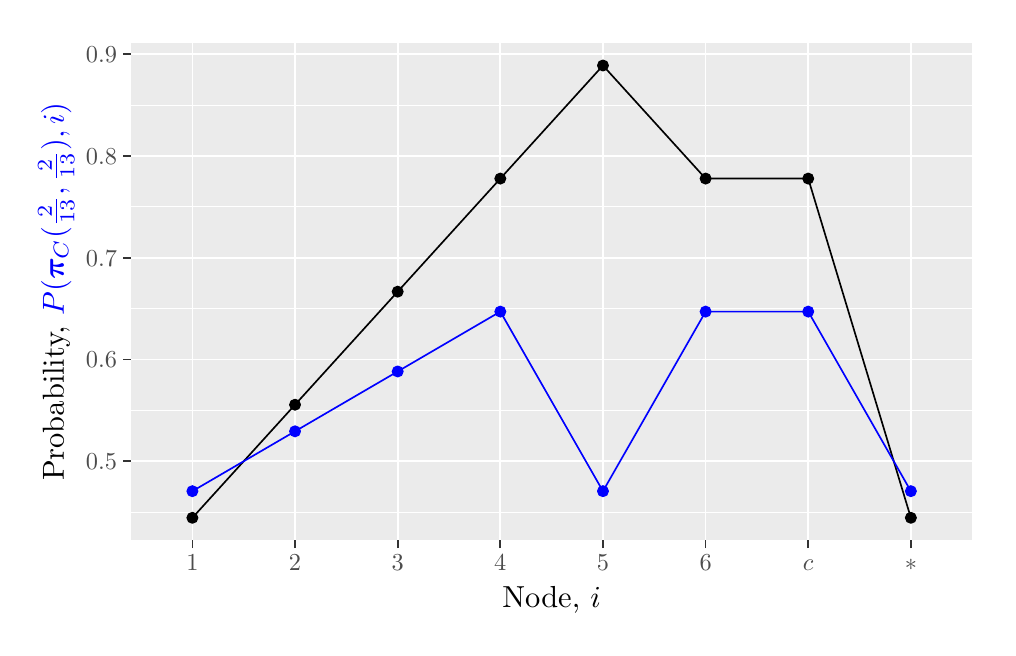
\begin{tikzpicture}[x=1pt,y=1pt]
\definecolor{fillColor}{RGB}{255,255,255}
\path[use as bounding box,fill=fillColor,fill opacity=0.00] (0,0) rectangle (346.90,216.81);
\begin{scope}
\path[clip] (  0.00,  0.00) rectangle (346.90,216.81);
\definecolor{drawColor}{RGB}{255,255,255}
\definecolor{fillColor}{RGB}{255,255,255}

\path[draw=drawColor,line width= 0.6pt,line join=round,line cap=round,fill=fillColor] (  0.00,  0.00) rectangle (346.90,216.81);
\end{scope}
\begin{scope}
\path[clip] ( 37.27, 31.53) rectangle (341.40,211.31);
\definecolor{fillColor}{gray}{0.92}

\path[fill=fillColor] ( 37.27, 31.53) rectangle (341.40,211.31);
\definecolor{drawColor}{RGB}{255,255,255}

\path[draw=drawColor,line width= 0.3pt,line join=round] ( 37.27, 41.75) --
	(341.40, 41.75);

\path[draw=drawColor,line width= 0.3pt,line join=round] ( 37.27, 78.52) --
	(341.40, 78.52);

\path[draw=drawColor,line width= 0.3pt,line join=round] ( 37.27,115.29) --
	(341.40,115.29);

\path[draw=drawColor,line width= 0.3pt,line join=round] ( 37.27,152.06) --
	(341.40,152.06);

\path[draw=drawColor,line width= 0.3pt,line join=round] ( 37.27,188.84) --
	(341.40,188.84);

\path[draw=drawColor,line width= 0.6pt,line join=round] ( 37.27, 60.13) --
	(341.40, 60.13);

\path[draw=drawColor,line width= 0.6pt,line join=round] ( 37.27, 96.90) --
	(341.40, 96.90);

\path[draw=drawColor,line width= 0.6pt,line join=round] ( 37.27,133.68) --
	(341.40,133.68);

\path[draw=drawColor,line width= 0.6pt,line join=round] ( 37.27,170.45) --
	(341.40,170.45);

\path[draw=drawColor,line width= 0.6pt,line join=round] ( 37.27,207.22) --
	(341.40,207.22);

\path[draw=drawColor,line width= 0.6pt,line join=round] ( 59.52, 31.53) --
	( 59.52,211.31);

\path[draw=drawColor,line width= 0.6pt,line join=round] ( 96.61, 31.53) --
	( 96.61,211.31);

\path[draw=drawColor,line width= 0.6pt,line join=round] (133.70, 31.53) --
	(133.70,211.31);

\path[draw=drawColor,line width= 0.6pt,line join=round] (170.79, 31.53) --
	(170.79,211.31);

\path[draw=drawColor,line width= 0.6pt,line join=round] (207.88, 31.53) --
	(207.88,211.31);

\path[draw=drawColor,line width= 0.6pt,line join=round] (244.97, 31.53) --
	(244.97,211.31);

\path[draw=drawColor,line width= 0.6pt,line join=round] (282.05, 31.53) --
	(282.05,211.31);

\path[draw=drawColor,line width= 0.6pt,line join=round] (319.14, 31.53) --
	(319.14,211.31);
\definecolor{drawColor}{RGB}{0,0,0}
\definecolor{fillColor}{RGB}{0,0,0}

\path[draw=drawColor,line width= 0.4pt,line join=round,line cap=round,fill=fillColor] ( 59.52, 39.70) circle (  1.96);

\path[draw=drawColor,line width= 0.4pt,line join=round,line cap=round,fill=fillColor] ( 96.61, 80.56) circle (  1.96);

\path[draw=drawColor,line width= 0.4pt,line join=round,line cap=round,fill=fillColor] (133.70,121.42) circle (  1.96);

\path[draw=drawColor,line width= 0.4pt,line join=round,line cap=round,fill=fillColor] (170.79,162.28) circle (  1.96);

\path[draw=drawColor,line width= 0.4pt,line join=round,line cap=round,fill=fillColor] (207.88,203.14) circle (  1.96);

\path[draw=drawColor,line width= 0.4pt,line join=round,line cap=round,fill=fillColor] (244.97,162.28) circle (  1.96);

\path[draw=drawColor,line width= 0.4pt,line join=round,line cap=round,fill=fillColor] (282.05,162.28) circle (  1.96);

\path[draw=drawColor,line width= 0.4pt,line join=round,line cap=round,fill=fillColor] (319.14, 39.70) circle (  1.96);

\path[draw=drawColor,line width= 0.6pt,line join=round] ( 59.52, 39.70) --
	( 96.61, 80.56) --
	(133.70,121.42) --
	(170.79,162.28) --
	(207.88,203.14) --
	(244.97,162.28) --
	(282.05,162.28) --
	(319.14, 39.70);
\definecolor{drawColor}{RGB}{0,0,255}
\definecolor{fillColor}{RGB}{0,0,255}

\path[draw=drawColor,line width= 0.4pt,line join=round,line cap=round,fill=fillColor] ( 59.52, 49.32) circle (  1.96);

\path[draw=drawColor,line width= 0.4pt,line join=round,line cap=round,fill=fillColor] ( 96.61, 70.95) circle (  1.96);

\path[draw=drawColor,line width= 0.4pt,line join=round,line cap=round,fill=fillColor] (133.70, 92.58) circle (  1.96);

\path[draw=drawColor,line width= 0.4pt,line join=round,line cap=round,fill=fillColor] (170.79,114.21) circle (  1.96);

\path[draw=drawColor,line width= 0.4pt,line join=round,line cap=round,fill=fillColor] (207.88, 49.32) circle (  1.96);

\path[draw=drawColor,line width= 0.4pt,line join=round,line cap=round,fill=fillColor] (244.97,114.21) circle (  1.96);

\path[draw=drawColor,line width= 0.4pt,line join=round,line cap=round,fill=fillColor] (282.05,114.21) circle (  1.96);

\path[draw=drawColor,line width= 0.4pt,line join=round,line cap=round,fill=fillColor] (319.14, 49.32) circle (  1.96);

\path[draw=drawColor,line width= 0.6pt,line join=round] ( 59.52, 49.32) --
	( 96.61, 70.95) --
	(133.70, 92.58) --
	(170.79,114.21) --
	(207.88, 49.32) --
	(244.97,114.21) --
	(282.05,114.21) --
	(319.14, 49.32);
\end{scope}
\begin{scope}
\path[clip] (  0.00,  0.00) rectangle (346.90,216.81);
\definecolor{drawColor}{gray}{0.30}

\node[text=drawColor,anchor=base east,inner sep=0pt, outer sep=0pt, scale=  0.88] at ( 32.32, 57.10) {0.5};

\node[text=drawColor,anchor=base east,inner sep=0pt, outer sep=0pt, scale=  0.88] at ( 32.32, 93.87) {0.6};

\node[text=drawColor,anchor=base east,inner sep=0pt, outer sep=0pt, scale=  0.88] at ( 32.32,130.65) {0.7};

\node[text=drawColor,anchor=base east,inner sep=0pt, outer sep=0pt, scale=  0.88] at ( 32.32,167.42) {0.8};

\node[text=drawColor,anchor=base east,inner sep=0pt, outer sep=0pt, scale=  0.88] at ( 32.32,204.19) {0.9};
\end{scope}
\begin{scope}
\path[clip] (  0.00,  0.00) rectangle (346.90,216.81);
\definecolor{drawColor}{gray}{0.20}

\path[draw=drawColor,line width= 0.6pt,line join=round] ( 34.52, 60.13) --
	( 37.27, 60.13);

\path[draw=drawColor,line width= 0.6pt,line join=round] ( 34.52, 96.90) --
	( 37.27, 96.90);

\path[draw=drawColor,line width= 0.6pt,line join=round] ( 34.52,133.68) --
	( 37.27,133.68);

\path[draw=drawColor,line width= 0.6pt,line join=round] ( 34.52,170.45) --
	( 37.27,170.45);

\path[draw=drawColor,line width= 0.6pt,line join=round] ( 34.52,207.22) --
	( 37.27,207.22);
\end{scope}
\begin{scope}
\path[clip] (  0.00,  0.00) rectangle (346.90,216.81);
\definecolor{drawColor}{gray}{0.20}

\path[draw=drawColor,line width= 0.6pt,line join=round] ( 59.52, 28.78) --
	( 59.52, 31.53);

\path[draw=drawColor,line width= 0.6pt,line join=round] ( 96.61, 28.78) --
	( 96.61, 31.53);

\path[draw=drawColor,line width= 0.6pt,line join=round] (133.70, 28.78) --
	(133.70, 31.53);

\path[draw=drawColor,line width= 0.6pt,line join=round] (170.79, 28.78) --
	(170.79, 31.53);

\path[draw=drawColor,line width= 0.6pt,line join=round] (207.88, 28.78) --
	(207.88, 31.53);

\path[draw=drawColor,line width= 0.6pt,line join=round] (244.97, 28.78) --
	(244.97, 31.53);

\path[draw=drawColor,line width= 0.6pt,line join=round] (282.05, 28.78) --
	(282.05, 31.53);

\path[draw=drawColor,line width= 0.6pt,line join=round] (319.14, 28.78) --
	(319.14, 31.53);
\end{scope}
\begin{scope}
\path[clip] (  0.00,  0.00) rectangle (346.90,216.81);
\definecolor{drawColor}{gray}{0.30}

\node[text=drawColor,anchor=base,inner sep=0pt, outer sep=0pt, scale=  0.88] at ( 59.52, 20.52) {$1$};

\node[text=drawColor,anchor=base,inner sep=0pt, outer sep=0pt, scale=  0.88] at ( 96.61, 20.52) {$2$};

\node[text=drawColor,anchor=base,inner sep=0pt, outer sep=0pt, scale=  0.88] at (133.70, 20.52) {$3$};

\node[text=drawColor,anchor=base,inner sep=0pt, outer sep=0pt, scale=  0.88] at (170.79, 20.52) {$4$};

\node[text=drawColor,anchor=base,inner sep=0pt, outer sep=0pt, scale=  0.88] at (207.88, 20.52) {$5$};

\node[text=drawColor,anchor=base,inner sep=0pt, outer sep=0pt, scale=  0.88] at (244.97, 20.52) {$6$};

\node[text=drawColor,anchor=base,inner sep=0pt, outer sep=0pt, scale=  0.88] at (282.05, 20.52) {$c$};

\node[text=drawColor,anchor=base,inner sep=0pt, outer sep=0pt, scale=  0.88] at (319.14, 20.52) {$*$};
\end{scope}
\begin{scope}
\path[clip] (  0.00,  0.00) rectangle (346.90,216.81);
\definecolor{drawColor}{RGB}{0,0,0}

\node[text=drawColor,anchor=base,inner sep=0pt, outer sep=0pt, scale=  1.10] at (189.33,  7.44) {Node, $i$};
\end{scope}
\begin{scope}
\path[clip] (  0.00,  0.00) rectangle (346.90,216.81);
\definecolor{drawColor}{RGB}{0,0,0}

\node[text=drawColor,rotate= 90.00,anchor=base,inner sep=0pt, outer sep=0pt, scale=  1.10] at ( 13.08,121.42) {Probability, \textcolor{blue}{$P(\bm{\pi}_{C}(\frac{2}{13},\frac{2}{13}),i)$}};
\end{scope}
\end{tikzpicture}

\end{center}
\caption{Interception probabilities of $S^5_{4}$ when $m=8$, with the \textcolor{blue}{blue Probabilities showing the Choosing Improvement Policy $\beta_{1} \left(\frac{2}{13},\frac{2}{13} \right)$}.}
\end{myfigure}

\begin{myfigure}
\begin{center}
% Created by tikzDevice version 0.10.1 on 2018-06-27 15:02:51
% !TEX encoding = UTF-8 Unicode
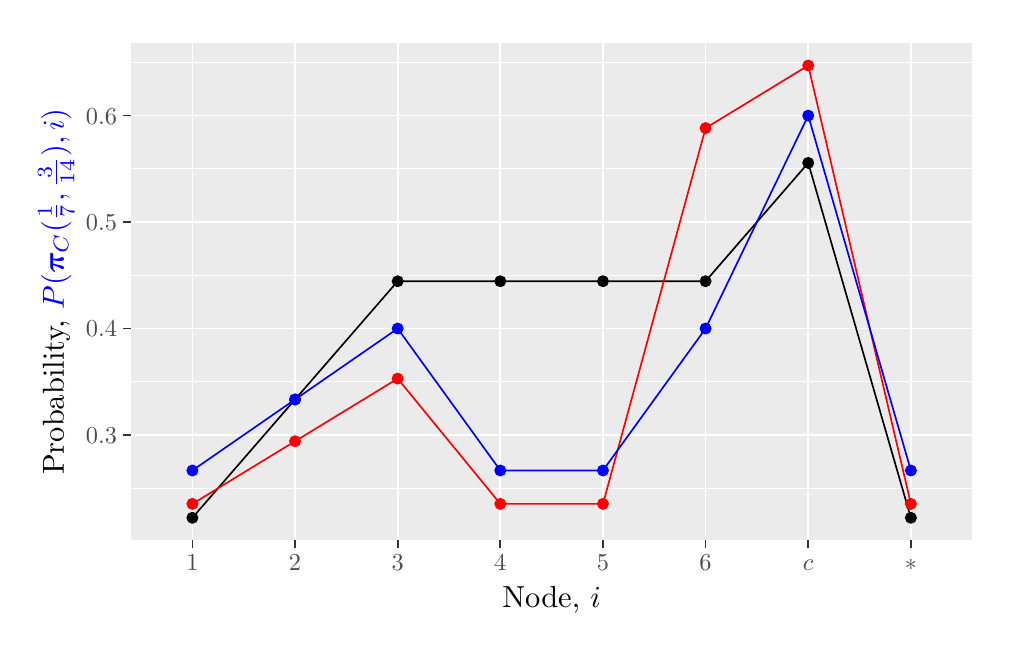
\begin{tikzpicture}[x=1pt,y=1pt]
\definecolor{fillColor}{RGB}{255,255,255}
\path[use as bounding box,fill=fillColor,fill opacity=0.00] (0,0) rectangle (346.90,216.81);
\begin{scope}
\path[clip] (  0.00,  0.00) rectangle (346.90,216.81);
\definecolor{drawColor}{RGB}{255,255,255}
\definecolor{fillColor}{RGB}{255,255,255}

\path[draw=drawColor,line width= 0.6pt,line join=round,line cap=round,fill=fillColor] (  0.00,  0.00) rectangle (346.90,216.81);
\end{scope}
\begin{scope}
\path[clip] ( 37.27, 31.53) rectangle (341.40,211.31);
\definecolor{fillColor}{gray}{0.92}

\path[fill=fillColor] ( 37.27, 31.53) rectangle (341.40,211.31);
\definecolor{drawColor}{RGB}{255,255,255}

\path[draw=drawColor,line width= 0.3pt,line join=round] ( 37.27, 50.39) --
	(341.40, 50.39);

\path[draw=drawColor,line width= 0.3pt,line join=round] ( 37.27, 88.86) --
	(341.40, 88.86);

\path[draw=drawColor,line width= 0.3pt,line join=round] ( 37.27,127.33) --
	(341.40,127.33);

\path[draw=drawColor,line width= 0.3pt,line join=round] ( 37.27,165.80) --
	(341.40,165.80);

\path[draw=drawColor,line width= 0.3pt,line join=round] ( 37.27,204.27) --
	(341.40,204.27);

\path[draw=drawColor,line width= 0.6pt,line join=round] ( 37.27, 69.62) --
	(341.40, 69.62);

\path[draw=drawColor,line width= 0.6pt,line join=round] ( 37.27,108.09) --
	(341.40,108.09);

\path[draw=drawColor,line width= 0.6pt,line join=round] ( 37.27,146.56) --
	(341.40,146.56);

\path[draw=drawColor,line width= 0.6pt,line join=round] ( 37.27,185.03) --
	(341.40,185.03);

\path[draw=drawColor,line width= 0.6pt,line join=round] ( 59.52, 31.53) --
	( 59.52,211.31);

\path[draw=drawColor,line width= 0.6pt,line join=round] ( 96.61, 31.53) --
	( 96.61,211.31);

\path[draw=drawColor,line width= 0.6pt,line join=round] (133.70, 31.53) --
	(133.70,211.31);

\path[draw=drawColor,line width= 0.6pt,line join=round] (170.79, 31.53) --
	(170.79,211.31);

\path[draw=drawColor,line width= 0.6pt,line join=round] (207.88, 31.53) --
	(207.88,211.31);

\path[draw=drawColor,line width= 0.6pt,line join=round] (244.96, 31.53) --
	(244.96,211.31);

\path[draw=drawColor,line width= 0.6pt,line join=round] (282.05, 31.53) --
	(282.05,211.31);

\path[draw=drawColor,line width= 0.6pt,line join=round] (319.14, 31.53) --
	(319.14,211.31);
\definecolor{drawColor}{RGB}{0,0,0}
\definecolor{fillColor}{RGB}{0,0,0}

\path[draw=drawColor,line width= 0.4pt,line join=round,line cap=round,fill=fillColor] ( 59.52, 39.70) circle (  1.96);

\path[draw=drawColor,line width= 0.4pt,line join=round,line cap=round,fill=fillColor] ( 96.61, 82.45) circle (  1.96);

\path[draw=drawColor,line width= 0.4pt,line join=round,line cap=round,fill=fillColor] (133.70,125.19) circle (  1.96);

\path[draw=drawColor,line width= 0.4pt,line join=round,line cap=round,fill=fillColor] (170.79,125.19) circle (  1.96);

\path[draw=drawColor,line width= 0.4pt,line join=round,line cap=round,fill=fillColor] (207.88,125.19) circle (  1.96);

\path[draw=drawColor,line width= 0.4pt,line join=round,line cap=round,fill=fillColor] (244.96,125.19) circle (  1.96);

\path[draw=drawColor,line width= 0.4pt,line join=round,line cap=round,fill=fillColor] (282.05,167.94) circle (  1.96);

\path[draw=drawColor,line width= 0.4pt,line join=round,line cap=round,fill=fillColor] (319.14, 39.70) circle (  1.96);

\path[draw=drawColor,line width= 0.6pt,line join=round] ( 59.52, 39.70) --
	( 96.61, 82.45) --
	(133.70,125.19) --
	(170.79,125.19) --
	(207.88,125.19) --
	(244.96,125.19) --
	(282.05,167.94) --
	(319.14, 39.70);
\definecolor{drawColor}{RGB}{255,0,0}
\definecolor{fillColor}{RGB}{255,0,0}

\path[draw=drawColor,line width= 0.4pt,line join=round,line cap=round,fill=fillColor] ( 59.52, 44.73) circle (  1.96);

\path[draw=drawColor,line width= 0.4pt,line join=round,line cap=round,fill=fillColor] ( 96.61, 67.36) circle (  1.96);

\path[draw=drawColor,line width= 0.4pt,line join=round,line cap=round,fill=fillColor] (133.70, 89.99) circle (  1.96);

\path[draw=drawColor,line width= 0.4pt,line join=round,line cap=round,fill=fillColor] (170.79, 44.73) circle (  1.96);

\path[draw=drawColor,line width= 0.4pt,line join=round,line cap=round,fill=fillColor] (207.88, 44.73) circle (  1.96);

\path[draw=drawColor,line width= 0.4pt,line join=round,line cap=round,fill=fillColor] (244.96,180.51) circle (  1.96);

\path[draw=drawColor,line width= 0.4pt,line join=round,line cap=round,fill=fillColor] (282.05,203.14) circle (  1.96);

\path[draw=drawColor,line width= 0.4pt,line join=round,line cap=round,fill=fillColor] (319.14, 44.73) circle (  1.96);

\path[draw=drawColor,line width= 0.6pt,line join=round] ( 59.52, 44.73) --
	( 96.61, 67.36) --
	(133.70, 89.99) --
	(170.79, 44.73) --
	(207.88, 44.73) --
	(244.96,180.51) --
	(282.05,203.14) --
	(319.14, 44.73);
\definecolor{drawColor}{RGB}{0,0,255}
\definecolor{fillColor}{RGB}{0,0,255}

\path[draw=drawColor,line width= 0.4pt,line join=round,line cap=round,fill=fillColor] ( 59.52, 56.80) circle (  1.96);

\path[draw=drawColor,line width= 0.4pt,line join=round,line cap=round,fill=fillColor] ( 96.61, 82.45) circle (  1.96);

\path[draw=drawColor,line width= 0.4pt,line join=round,line cap=round,fill=fillColor] (133.70,108.09) circle (  1.96);

\path[draw=drawColor,line width= 0.4pt,line join=round,line cap=round,fill=fillColor] (170.79, 56.80) circle (  1.96);

\path[draw=drawColor,line width= 0.4pt,line join=round,line cap=round,fill=fillColor] (207.88, 56.80) circle (  1.96);

\path[draw=drawColor,line width= 0.4pt,line join=round,line cap=round,fill=fillColor] (244.96,108.09) circle (  1.96);

\path[draw=drawColor,line width= 0.4pt,line join=round,line cap=round,fill=fillColor] (282.05,185.03) circle (  1.96);

\path[draw=drawColor,line width= 0.4pt,line join=round,line cap=round,fill=fillColor] (319.14, 56.80) circle (  1.96);

\path[draw=drawColor,line width= 0.6pt,line join=round] ( 59.52, 56.80) --
	( 96.61, 82.45) --
	(133.70,108.09) --
	(170.79, 56.80) --
	(207.88, 56.80) --
	(244.96,108.09) --
	(282.05,185.03) --
	(319.14, 56.80);
\end{scope}
\begin{scope}
\path[clip] (  0.00,  0.00) rectangle (346.90,216.81);
\definecolor{drawColor}{gray}{0.30}

\node[text=drawColor,anchor=base east,inner sep=0pt, outer sep=0pt, scale=  0.88] at ( 32.32, 66.59) {0.3};

\node[text=drawColor,anchor=base east,inner sep=0pt, outer sep=0pt, scale=  0.88] at ( 32.32,105.06) {0.4};

\node[text=drawColor,anchor=base east,inner sep=0pt, outer sep=0pt, scale=  0.88] at ( 32.32,143.53) {0.5};

\node[text=drawColor,anchor=base east,inner sep=0pt, outer sep=0pt, scale=  0.88] at ( 32.32,182.00) {0.6};
\end{scope}
\begin{scope}
\path[clip] (  0.00,  0.00) rectangle (346.90,216.81);
\definecolor{drawColor}{gray}{0.20}

\path[draw=drawColor,line width= 0.6pt,line join=round] ( 34.52, 69.62) --
	( 37.27, 69.62);

\path[draw=drawColor,line width= 0.6pt,line join=round] ( 34.52,108.09) --
	( 37.27,108.09);

\path[draw=drawColor,line width= 0.6pt,line join=round] ( 34.52,146.56) --
	( 37.27,146.56);

\path[draw=drawColor,line width= 0.6pt,line join=round] ( 34.52,185.03) --
	( 37.27,185.03);
\end{scope}
\begin{scope}
\path[clip] (  0.00,  0.00) rectangle (346.90,216.81);
\definecolor{drawColor}{gray}{0.20}

\path[draw=drawColor,line width= 0.6pt,line join=round] ( 59.52, 28.78) --
	( 59.52, 31.53);

\path[draw=drawColor,line width= 0.6pt,line join=round] ( 96.61, 28.78) --
	( 96.61, 31.53);

\path[draw=drawColor,line width= 0.6pt,line join=round] (133.70, 28.78) --
	(133.70, 31.53);

\path[draw=drawColor,line width= 0.6pt,line join=round] (170.79, 28.78) --
	(170.79, 31.53);

\path[draw=drawColor,line width= 0.6pt,line join=round] (207.88, 28.78) --
	(207.88, 31.53);

\path[draw=drawColor,line width= 0.6pt,line join=round] (244.96, 28.78) --
	(244.96, 31.53);

\path[draw=drawColor,line width= 0.6pt,line join=round] (282.05, 28.78) --
	(282.05, 31.53);

\path[draw=drawColor,line width= 0.6pt,line join=round] (319.14, 28.78) --
	(319.14, 31.53);
\end{scope}
\begin{scope}
\path[clip] (  0.00,  0.00) rectangle (346.90,216.81);
\definecolor{drawColor}{gray}{0.30}

\node[text=drawColor,anchor=base,inner sep=0pt, outer sep=0pt, scale=  0.88] at ( 59.52, 20.52) {$1$};

\node[text=drawColor,anchor=base,inner sep=0pt, outer sep=0pt, scale=  0.88] at ( 96.61, 20.52) {$2$};

\node[text=drawColor,anchor=base,inner sep=0pt, outer sep=0pt, scale=  0.88] at (133.70, 20.52) {$3$};

\node[text=drawColor,anchor=base,inner sep=0pt, outer sep=0pt, scale=  0.88] at (170.79, 20.52) {$4$};

\node[text=drawColor,anchor=base,inner sep=0pt, outer sep=0pt, scale=  0.88] at (207.88, 20.52) {$5$};

\node[text=drawColor,anchor=base,inner sep=0pt, outer sep=0pt, scale=  0.88] at (244.96, 20.52) {$6$};

\node[text=drawColor,anchor=base,inner sep=0pt, outer sep=0pt, scale=  0.88] at (282.05, 20.52) {$c$};

\node[text=drawColor,anchor=base,inner sep=0pt, outer sep=0pt, scale=  0.88] at (319.14, 20.52) {$*$};
\end{scope}
\begin{scope}
\path[clip] (  0.00,  0.00) rectangle (346.90,216.81);
\definecolor{drawColor}{RGB}{0,0,0}

\node[text=drawColor,anchor=base,inner sep=0pt, outer sep=0pt, scale=  1.10] at (189.33,  7.44) {Node, $i$};
\end{scope}
\begin{scope}
\path[clip] (  0.00,  0.00) rectangle (346.90,216.81);
\definecolor{drawColor}{RGB}{0,0,0}

\node[text=drawColor,rotate= 90.00,anchor=base,inner sep=0pt, outer sep=0pt, scale=  1.10] at ( 13.08,121.42) {Probability, \textcolor{blue}{$P(\bm{\pi}_{C}(\frac{1}{7},\frac{3}{14}),i)$}};
\end{scope}
\end{tikzpicture}

\end{center}
\caption{Interception probabilities of $S^5_{4}$ when $m=4$, with the \textcolor{red}{red Probabilities showing the Naive Improvement Policy $\alpha \left(\frac{2}{17},\frac{6}{17} \right)$} and the \textcolor{blue}{blue Probabilities showing the Choosing Improvement Policy $\beta_{2} \left(\frac{1}{7},\frac{3}{14} \right)$}.}
\end{myfigure}

It is conjectured in our future work (see section \ref{Section:Further solutions for elongated trees}) that the bound $V \geq \frac{2m}{2(n+k)+m(1+\frac{n-1}{\hat{m}})}$ is used in the region of $m < 2(k+1)$. When $m$ is even this bound becomes $V \geq \frac{2m}{2(2n+k-1)+m}$ which we will conjecture is tight with a multitude of attack strategies, however when $m$ is odd due to the half-length, $\hat{m} \equiv \floor{\frac{m}{2}}$, it makes the bound higher than when $m$ is even, which will not be tight. We suggest some slight alteration when $m$ is odd, but have to drop the use of end-covering cycles (we leave this idea to section \ref{Section:Further solutions for elongated trees})

We will now deal with the case of $m \leq 2(n-1)$, so that all $*$'s nodes cannot be covered in one end-covering cycle. First looking at the $m=2k+1,2k$,  we notice that by simplification of $S^{k}_{n}$ into $L_{k+1}$ and $S_{n-1}$ we get the bound $V \geq \frac{1}{1+\frac{2(n-1)}{m}}=\frac{m}{m+2(n-1)}$.

When $m=2k+1$ we can propose an attack that `augments' the time-delayed which simply removes one attack placed at $1$. That is to place attacks at node $1$ starting at times, $\tau,...,\tau+2k$ and $*$ nodes starting at times $\tau+k,\tau+k+1$ (equally we could use $\tau+k-1,\tau+k$) all with equal probability. Similarly if $m=2k$ we augment it to node $1$ at times $\tau,...,\tau+2k-1$ and $*$ nodes at times $\tau+k-1,\tau+k$ all with equal probability.

\begin{lemma}
Using the `augmented' time-delayed we propose the attacker can get a bound of $V \leq \frac{m}{m+2(n-1)}$ and hence $V(S_{n}^{k})=\frac{m}{m+2(n-1)}$ for $m=2k+1,2k$
\end{lemma}

The idea of the proof for the `augmented' time-delayed attack is the same as the time-delayed attack , but with a reduced number of attacks at node $1$, to make sure the patroller can only get $m$ by waiting here. No significant alteration to the proof takes place.

We leave the rest of the idea to solve in the region $m < 2(k+1)$ to \ref{Section:Further solutions for elongated trees}, but respect that it may be difficult and careful consideration of attacker strategies may need to be taken when the random oscillation is not the best strategy for the patroller. This is analagous to the situtation in the region of $S_{5}$ for the line (see section 5 in \cite{Lin2013}).

\subsection{Generalising the star graph}
For now we will set aside the difficulty with the elongated star and look at generalising it, in which we can solve for values of $m$ which match the random oscillation.We generalise further by allowing a general star graph to have all external nodes any distance from the centre node, again performed by subdivision of the edge an appropriate number of times.

\begin{definition}[General star graph]
The \textit{general star graph}, $S^{\bm{k}}_{n}$ ($\bm{k} \in \mathbb{N}^{h}$) is made from $S_{n}$, by performing subdivision on $h$ of the  initial edges each repeated $k_{i}$ for each edge for $i=1,...,h$ . 
\end{definition}

\begin{note}
For ease of notation we will use the above format, but will understand that using $k_{i}=0$ is a valid construction, so we can imagine that $\bm{k} \in \mathbb{N}^n$.
For ease of notation we will also define define $ |\bm{k}| \equiv \sum\limits_{i=0}^{i=h} k_{i}$ and $ k_{\max} \equiv \max\limits_{i=1,2,..,h} k_{i}$.
\end{note}

The labelling will be done as in figure \ref{Figure:Example of generalised labelling} and note that all nodes with the same label are symmetric and must be treated as such. We will refer to the branch made by $k_{i}$ subdivisions of the edge as the $i$\textsuperscript{th} branch, which is made up of the nodes $n_{j,i}$ for $j=1,...,k_{i}+1$, so $n_{j,i}$ is $j$\textsuperscript{th} node on $i$\textsuperscript{th} branch).

\begin{myfigure}
\begin{center}
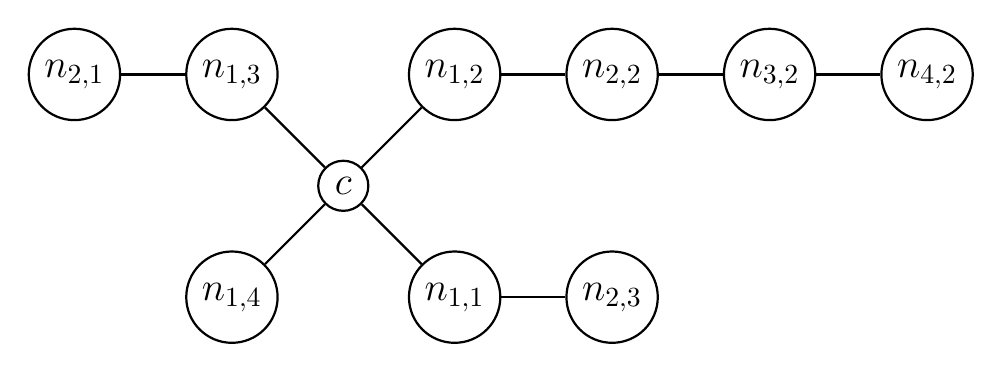
\begin{tikzpicture}[-,auto,node distance=2cm,
                    thick,main node/.style={circle,draw,font=\sffamily\Large\bfseries}]

  \node[main node] (1) {$c$};
  \node[main node] (2) [below left of=1] {$n_{1,4}$};
  \node[main node] (3) [below right of=1] {$n_{1,1}$};
  \node[main node] (4) [above left of=1] {$n_{1,3}$};
  \node[main node] (5) [above right of=1] {$n_{1,2}$};
  \node[main node] (6) [right of=5]  {$n_{2,2}$};
  \node[main node] (7) [right of=6]  {$n_{3,2}$};
  \node[main node] (8) [right of=7]  {$n_{4,2}$};
  \node[main node] (9) [left of=4] {$n_{2,1}$};
  \node[main node] (10) [right of=3] {$n_{2,3}$};
  
  \path[every node/.style={font=\sffamily}]
    (1) edge  (2)
    edge(3)
    edge(4)
    edge(5)
    (5) edge (6)
    (6) edge (7)
    (7) edge (8)
    (9) edge (4)
    (10) edge (3);
    
\end{tikzpicture}
\end{center}
\caption{Labelling of $S^{1,3,1}_{4}$.}
\label{Figure:Example of generalised labelling}
\end{myfigure}

To start our analysis of this graph, we will look at an expanded graph which can be simplified down to our general star graph. Consider the cyclic graph $C_{2(n+|k|)}$, this can simplified to $S^{\bm{k}}_{n}$ by node identification. The identification mapping is analogous to that of the elongated star graph's simplification from a cyclic graph; Internal branch nodes are seen twice and the centre node is seen on every return, so the cycle graph can be made from this construction as in the example in figure \ref{Figure:Example of simplification to general star graph}.

The mapping is done as such:
\begin{itemize}
\item The centre is identified from nodes $1,1+2(k_{1}+1),1+2(\sum\limits_{i=1}^{2} (k_{i}+1)),...,1+2(\sum\limits_{i=1}^{h}(k_{i}+1),1+2(|k|+h)+2),...,1+2(|k|+h)+2(n-h)$

\item The first branch is identified from the nodes between $2$ and $2(k_{1}+1)$ (Inclusive). $n_{1,i}$ for $i=1,...,k_{1}$ are identified by the two nodes $i+1$ and $2k_{1}+3-i$ , the node $n_{1,k_{1}+1}$ is identified by the one node $k_{1}+2$.

\item The $j$\textsuperscript{th} branch is identified from nodes between $2(\sum\limits_{i=1}^{j-1} (k_{i}+1)))$ and $2(\sum\limits_{i=1}^{j} (k_{i}+1)))$ (Inclusive). $n_{j,i}$ for $i=1,....,k_{j}$ are identified by the two nodes $2(\sum\limits_{i=1}^{j-1} (k_{i}+1)))+(i-1)$ and $2(\sum\limits_{i=1}^{j} (k_{i}+1)))-(i-1)$ , the node $n_{j,k_{j}+1}$ is identified by the one node $2(\sum\limits_{i=1}^{j-1} (k_{i}+1)))+k_{j}$.
\end{itemize}

This simplification mapping gives rise to the general random oscillation strategy (analogous to random oscillation on the elongated star).

\begin{definition}[General random oscillation]
The \textit{oscillation} on $S^{\bm{k}}_{n}$ is any embedded Hamiltonian patrol on $C_{2(n+|k|)}$ under the simplification above. The \textit{random oscillation} on $S^{\bm{k}}_{n}$ is the embedded random Hamiltonian patrol on $C_{2(n+|k|)}$ under the simplification above.
\end{definition}

\begin{lemma}
For $m < 2(n+|k|)$ following the random oscillation
$$V(S^{\bm{k}}_{n}) \geq V(C_{2(n+|k|)})=\frac{m}{2(n+|k|)}$$
and if $m \geq 2(n+|k|)$ then $V(S^{\bm{k}}_{n})=1$, achieved by any oscillation. 
\end{lemma}

The proof is straight forward by the application of the simplification (Lemma 1 (4) in \cite{Alpern2011}) and the Hamiltonian solution(Theorem 13 (1) in \cite{Alpern2011}).

\begin{myfigure}
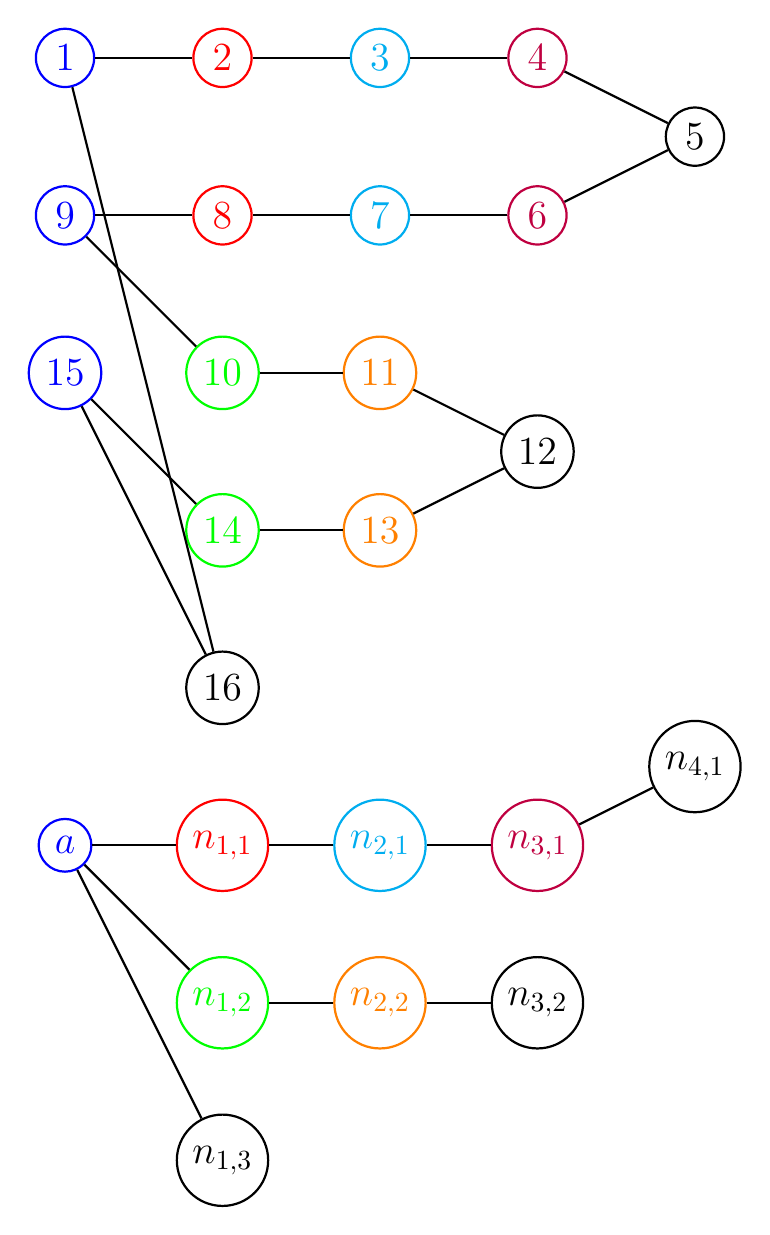
\begin{tikzpicture}[-,auto,node distance=2cm,
                    thick,main node/.style={circle,draw,font=\sffamily\Large\bfseries}]

  \node[main node,color=blue] (1) {$1$};
  \node[main node,color=blue] (2) [below of=1] {$9$};
  \node[main node,color=blue] (3) [below of=2] {$15$};
  \node[main node,color=red] (4) [right of=1] {$2$};
  \node[main node,color=red] (5) [right of=2]  {$8$};
  \node[main node,color=green] (6) [right of=3]  {$10$};
  \node[main node,color=green] (7) [below of=6]  {$14$};
  \node[main node] (13) [below of=7] {$16$};
  \node[main node,color=cyan] (8) [right of=4]  {$3$};
  \node[main node,color=purple] (9) [right of=8]  {$4$};
  \node[main node,color=cyan] (10) [right of=5]  {$7$};
  \node[main node,color=purple] (11) [right of=10]  {$6$};
  \node[main node] at (8,-1) (12)  {$5$};
  \node[main node,color=orange] (14) [right of=6] {$11$};
  \node[main node,color=orange] (15) [right of=7] {$13$};
  \node[main node] at (6,-5) (16) {$12$};

  \path[every node/.style={font=\sffamily}]
    (1) edge  (4)
    (2) edge  (5)
        edge  (6)
    (3) edge  (7)
    
    (4) edge (8)
    (13) edge (3)
    (13) edge (1)
    (8) edge (9)
    (9) edge (12)
    (12) edge (11)
    (11) edge (10)
    (10) edge (5)
    (6) edge (14)
    (7) edge (15)
    (14) edge (16)
    (15) edge (16);
  
  \node[main node,color=blue] (13) [below of=3,node distance=6cm] {$a$};
  \node[main node,color=red] (14) [right of=13] {$n_{1,1}$};
  \node[main node,color=green] (15) [below of=14] {$n_{1,2}$};
  \node[main node] (16) [below of=15] {$n_{1,3}$};
  \node[main node,color=cyan] (17) [right of=14] {$n_{2,1}$};
  \node[main node,color=purple] (18) [right of=17] {$n_{3,1}$};
  \node[main node] at (8,-9) (19) {$n_{4,1}$};      
  \node[main node,color=orange] (20) [right of=15] {$n_{2,2}$};
  \node[main node] (21) [right of=20] {$n_{3,2}$}; 
   
   \path[every node/.style={font=\sffamily}]
   (13) edge (14)
   edge (15)
   edge (16)
   (14) edge (17)
   (17) edge (18)
   (18) edge (19)
   (15) edge (20)
   (20) edge (21);
  
\end{tikzpicture}
\caption{Simplification of $C_{16}$ to $S^{3,2}_{3}$.}
\label{Figure:Example of simplification to general star graph}
\end{myfigure}

We will match the oscillation bound of $\frac{m}{2(n+|k|)}$, by further extending the time-delayed attack into the type-delayed attack, which will consider the length of the branches as the key to spacing out the attacks in time.

\begin{definition}[Node types]
A \textit{type} $i$ node, is an external node which has been extended $i$ times, that is the branch length. Then $k_{\max}$ is the maximum node type for $S_{n}^{\bm{k}}$.
\end{definition}

\begin{definition}[Type-delayed attack]
Let the \textit{type-delayed attack}, be the attack that attacks at a type $i$ node with probability $\frac{i+1}{\denominator}$ $\forall \, i$. For a fixed attack interval $I$, the attacks at a type $i$ node choose an interval from the following with equal probability: $I+(k_{max}-i),I+(k_{max}-i)+1,...,I+k_{max}+i+1$ $\forall \, i$ (i.e starting attacks at a type $i$ node at times $\tau+(k_{max}-i)+1,...,\tau+(k_{max}+i)+1$).
\end{definition}

A diagram showing how potential attacks are spaced out in time, for each node of a given type, can be seen in figure \ref{Figure:Time spacing of the type-delayed attack}.

\begin{myfigure}
\begin{center}
\resizebox{\linewidth}{!}{
\begin{tikzpicture}
 %Drawing Bottom Axis
 \draw[->] (-7,0) -- (7,0);
 \node (timelabel) [shift={(0.2,0)}] at (7,0) {$t$};
 
 
 \draw (-6.5,0.2) -- (-6.5,-0.2);
 \draw (6.5,0.2) -- (6.5,-0.2);
 
 \node (labelc1) at (-6.5,-0.5) {$\tau$};
 \node (labelc2) at (6.5,-0.5) {$\tau+2k_{max}+1$};
 
 \node[cross=5pt,red] (c1) at (-6.5,0.5) {};
 \node[cross=5pt,red] (c2) at (6.5,0.5) {};
 \draw[dashed] (c1) -- (c2);
 \node (linelabel1) at (-8,0.5) {Type $k_{max}$};
 
 
  \draw (-6,0.2) -- (-6,-0.2);
 \draw (6,0.2) -- (6,-0.2);
 
 %\node (labelc1) at (-5.5,-0.5) {$\tau+1$};
 %\node (labelc2) at (5.5,-0.5) {$\tau+2k_{max}-1$};
 
 \node[cross=5pt,red] (c1) at (-6,1.5) {};
 \node[cross=5pt,red] (c2) at (6,1.5) {};
 \draw[dashed] (c1) -- (c2);
 \node (linelabel1) at (-7.5,1.5) {Type $k_{max}-1$};
 
 
 
 \draw[decorate sep={2mm}{4mm},fill] (0,3.5) -- (0,2);

  \draw (-1.5,0.2) -- (-1.5,-0.2);
 \draw (1.5,0.2) -- (1.5,-0.2);
 
 %\node (labelc1) at (-5.5,-0.5) {$\tau+1$};
 %\node (labelc2) at (5.5,-0.5) {$\tau+2k_{max}-1$};
 
 \node[cross=5pt,red] (c1) at (-1.5,4) {};
 \node[cross=5pt,red] (c2) at (1.5,4) {};
 \draw[dashed] (c1) -- (c2);
 \node (linelabel1) at (-2.3,4) {Type $1$};
 
 \draw (-1,0.2) -- (-1,-0.2);
 \draw (1,0.2) -- (1,-0.2);
 
  \node (labelc3) at (-1,-0.5) {$\tau+k_{max}$};
 \node (labelc4) at (1,-0.5) {$\tau+k_{max}+1$};
 
 \node[cross=5pt,red] (c3) at (-1,5) {};
 \node[cross=5pt,red] (c4) at (1,5) {};
 \draw[dashed] (c3) -- (c4);
 \node (linelabel1) at (-1.9,5) {Type $0$}; 

\end{tikzpicture}
}
\end{center}
\caption{Time spacing of the type-delayed attack.}
\label{Figure:Time spacing of the type-delayed attack}
\end{myfigure}

\begin{theorem}
When $T \geq m+2k_{max}$, the upper bound is
$$V(S_{n}^{\bm{k}}) \leq \max \left\{ \frac{k_{max}+1}{\denominator} , \frac{m}{2 \left( \denominator \right)} \right\}$$
guaranteed by the type-delayed attack.
\end{theorem}

We leave the proof of this

\begin{corollary}[Solution in $m \geq 2(k_{max}+1)$]
When $T \geq m+2k_{max}$, by the attack using the type-delayed attack and the patroller using the random oscillation we achieve the value, when $2(k_{max}+1) \leq m \leq 2(n+|\bm{k}|)$,
$$V= \frac{m}{2(n+|\bm{k}|)} $$
and when $m > 2(n+|\bm{k}|)$ then $V=1$.
\end{corollary}

\begin{myfigure}
\begin{center}
% Created by tikzDevice version 0.10.1 on 2018-02-08 14:18:15
% !TEX encoding = UTF-8 Unicode
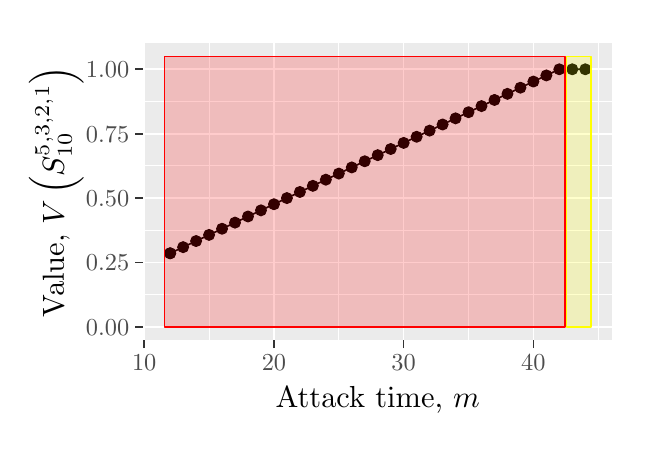
\begin{tikzpicture}[x=1pt,y=1pt]
\definecolor{fillColor}{RGB}{255,255,255}
\path[use as bounding box,fill=fillColor,fill opacity=0.00] (0,0) rectangle (216.81,144.54);
\begin{scope}
\path[clip] (  0.00,  0.00) rectangle (216.81,144.54);
\definecolor{drawColor}{RGB}{255,255,255}
\definecolor{fillColor}{RGB}{255,255,255}

\path[draw=drawColor,line width= 0.6pt,line join=round,line cap=round,fill=fillColor] (  0.00,  0.00) rectangle (216.81,144.54);
\end{scope}
\begin{scope}
\path[clip] ( 41.67, 31.53) rectangle (211.31,139.04);
\definecolor{fillColor}{gray}{0.92}

\path[fill=fillColor] ( 41.67, 31.53) rectangle (211.31,139.04);
\definecolor{drawColor}{RGB}{255,255,255}

\path[draw=drawColor,line width= 0.3pt,line join=round] ( 41.67, 48.05) --
	(211.31, 48.05);

\path[draw=drawColor,line width= 0.3pt,line join=round] ( 41.67, 71.32) --
	(211.31, 71.32);

\path[draw=drawColor,line width= 0.3pt,line join=round] ( 41.67, 94.59) --
	(211.31, 94.59);

\path[draw=drawColor,line width= 0.3pt,line join=round] ( 41.67,117.86) --
	(211.31,117.86);

\path[draw=drawColor,line width= 0.3pt,line join=round] ( 65.55, 31.53) --
	( 65.55,139.04);

\path[draw=drawColor,line width= 0.3pt,line join=round] (112.43, 31.53) --
	(112.43,139.04);

\path[draw=drawColor,line width= 0.3pt,line join=round] (159.30, 31.53) --
	(159.30,139.04);

\path[draw=drawColor,line width= 0.3pt,line join=round] (206.18, 31.53) --
	(206.18,139.04);

\path[draw=drawColor,line width= 0.6pt,line join=round] ( 41.67, 36.42) --
	(211.31, 36.42);

\path[draw=drawColor,line width= 0.6pt,line join=round] ( 41.67, 59.69) --
	(211.31, 59.69);

\path[draw=drawColor,line width= 0.6pt,line join=round] ( 41.67, 82.96) --
	(211.31, 82.96);

\path[draw=drawColor,line width= 0.6pt,line join=round] ( 41.67,106.23) --
	(211.31,106.23);

\path[draw=drawColor,line width= 0.6pt,line join=round] ( 41.67,129.50) --
	(211.31,129.50);

\path[draw=drawColor,line width= 0.6pt,line join=round] ( 42.11, 31.53) --
	( 42.11,139.04);

\path[draw=drawColor,line width= 0.6pt,line join=round] ( 88.99, 31.53) --
	( 88.99,139.04);

\path[draw=drawColor,line width= 0.6pt,line join=round] (135.86, 31.53) --
	(135.86,139.04);

\path[draw=drawColor,line width= 0.6pt,line join=round] (182.74, 31.53) --
	(182.74,139.04);
\definecolor{drawColor}{RGB}{0,0,0}
\definecolor{fillColor}{RGB}{0,0,0}

\path[draw=drawColor,line width= 0.4pt,line join=round,line cap=round,fill=fillColor] (196.80,129.50) circle (  1.96);

\path[draw=drawColor,line width= 0.4pt,line join=round,line cap=round,fill=fillColor] (201.49,129.50) circle (  1.96);

\path[draw=drawColor,line width= 0.4pt,line join=round,line cap=round,fill=fillColor] ( 51.49, 63.01) circle (  1.96);

\path[draw=drawColor,line width= 0.4pt,line join=round,line cap=round,fill=fillColor] ( 56.17, 65.23) circle (  1.96);

\path[draw=drawColor,line width= 0.4pt,line join=round,line cap=round,fill=fillColor] ( 60.86, 67.44) circle (  1.96);

\path[draw=drawColor,line width= 0.4pt,line join=round,line cap=round,fill=fillColor] ( 65.55, 69.66) circle (  1.96);

\path[draw=drawColor,line width= 0.4pt,line join=round,line cap=round,fill=fillColor] ( 70.24, 71.88) circle (  1.96);

\path[draw=drawColor,line width= 0.4pt,line join=round,line cap=round,fill=fillColor] ( 74.92, 74.09) circle (  1.96);

\path[draw=drawColor,line width= 0.4pt,line join=round,line cap=round,fill=fillColor] ( 79.61, 76.31) circle (  1.96);

\path[draw=drawColor,line width= 0.4pt,line join=round,line cap=round,fill=fillColor] ( 84.30, 78.53) circle (  1.96);

\path[draw=drawColor,line width= 0.4pt,line join=round,line cap=round,fill=fillColor] ( 88.99, 80.74) circle (  1.96);

\path[draw=drawColor,line width= 0.4pt,line join=round,line cap=round,fill=fillColor] ( 93.67, 82.96) circle (  1.96);

\path[draw=drawColor,line width= 0.4pt,line join=round,line cap=round,fill=fillColor] ( 98.36, 85.17) circle (  1.96);

\path[draw=drawColor,line width= 0.4pt,line join=round,line cap=round,fill=fillColor] (103.05, 87.39) circle (  1.96);

\path[draw=drawColor,line width= 0.4pt,line join=round,line cap=round,fill=fillColor] (107.74, 89.61) circle (  1.96);

\path[draw=drawColor,line width= 0.4pt,line join=round,line cap=round,fill=fillColor] (112.43, 91.82) circle (  1.96);

\path[draw=drawColor,line width= 0.4pt,line join=round,line cap=round,fill=fillColor] (117.11, 94.04) circle (  1.96);

\path[draw=drawColor,line width= 0.4pt,line join=round,line cap=round,fill=fillColor] (121.80, 96.26) circle (  1.96);

\path[draw=drawColor,line width= 0.4pt,line join=round,line cap=round,fill=fillColor] (126.49, 98.47) circle (  1.96);

\path[draw=drawColor,line width= 0.4pt,line join=round,line cap=round,fill=fillColor] (131.18,100.69) circle (  1.96);

\path[draw=drawColor,line width= 0.4pt,line join=round,line cap=round,fill=fillColor] (135.86,102.90) circle (  1.96);

\path[draw=drawColor,line width= 0.4pt,line join=round,line cap=round,fill=fillColor] (140.55,105.12) circle (  1.96);

\path[draw=drawColor,line width= 0.4pt,line join=round,line cap=round,fill=fillColor] (145.24,107.34) circle (  1.96);

\path[draw=drawColor,line width= 0.4pt,line join=round,line cap=round,fill=fillColor] (149.93,109.55) circle (  1.96);

\path[draw=drawColor,line width= 0.4pt,line join=round,line cap=round,fill=fillColor] (154.61,111.77) circle (  1.96);

\path[draw=drawColor,line width= 0.4pt,line join=round,line cap=round,fill=fillColor] (159.30,113.99) circle (  1.96);

\path[draw=drawColor,line width= 0.4pt,line join=round,line cap=round,fill=fillColor] (163.99,116.20) circle (  1.96);

\path[draw=drawColor,line width= 0.4pt,line join=round,line cap=round,fill=fillColor] (168.68,118.42) circle (  1.96);

\path[draw=drawColor,line width= 0.4pt,line join=round,line cap=round,fill=fillColor] (173.36,120.63) circle (  1.96);

\path[draw=drawColor,line width= 0.4pt,line join=round,line cap=round,fill=fillColor] (178.05,122.85) circle (  1.96);

\path[draw=drawColor,line width= 0.4pt,line join=round,line cap=round,fill=fillColor] (182.74,125.07) circle (  1.96);

\path[draw=drawColor,line width= 0.4pt,line join=round,line cap=round,fill=fillColor] (187.43,127.28) circle (  1.96);

\path[draw=drawColor,line width= 0.4pt,line join=round,line cap=round,fill=fillColor] (192.11,129.50) circle (  1.96);

\path[draw=drawColor,line width= 0.4pt,line join=round,line cap=round,fill=fillColor] ( 51.49, 63.01) circle (  1.96);

\path[draw=drawColor,line width= 0.6pt,line join=round] ( 51.49, 63.01) --
	( 51.49, 63.01) --
	( 56.17, 65.23) --
	( 60.86, 67.44) --
	( 65.55, 69.66) --
	( 70.24, 71.88) --
	( 74.92, 74.09) --
	( 79.61, 76.31) --
	( 84.30, 78.53) --
	( 88.99, 80.74) --
	( 93.67, 82.96) --
	( 98.36, 85.17) --
	(103.05, 87.39) --
	(107.74, 89.61) --
	(112.43, 91.82) --
	(117.11, 94.04) --
	(121.80, 96.26) --
	(126.49, 98.47) --
	(131.18,100.69) --
	(135.86,102.90) --
	(140.55,105.12) --
	(145.24,107.34) --
	(149.93,109.55) --
	(154.61,111.77) --
	(159.30,113.99) --
	(163.99,116.20) --
	(168.68,118.42) --
	(173.36,120.63) --
	(178.05,122.85) --
	(182.74,125.07) --
	(187.43,127.28) --
	(192.11,129.50) --
	(196.80,129.50) --
	(201.49,129.50);
\definecolor{drawColor}{RGB}{255,255,0}
\definecolor{fillColor}{RGB}{255,255,0}

\path[draw=drawColor,line width= 0.6pt,line join=round,fill=fillColor,fill opacity=0.20] (194.69, 36.42) rectangle (203.60,134.15);
\definecolor{drawColor}{RGB}{255,0,0}
\definecolor{fillColor}{RGB}{255,0,0}

\path[draw=drawColor,line width= 0.6pt,line join=round,fill=fillColor,fill opacity=0.20] ( 49.38, 36.42) rectangle (194.22,134.15);
\end{scope}
\begin{scope}
\path[clip] (  0.00,  0.00) rectangle (216.81,144.54);
\definecolor{drawColor}{gray}{0.30}

\node[text=drawColor,anchor=base east,inner sep=0pt, outer sep=0pt, scale=  0.88] at ( 36.72, 33.39) {0.00};

\node[text=drawColor,anchor=base east,inner sep=0pt, outer sep=0pt, scale=  0.88] at ( 36.72, 56.66) {0.25};

\node[text=drawColor,anchor=base east,inner sep=0pt, outer sep=0pt, scale=  0.88] at ( 36.72, 79.93) {0.50};

\node[text=drawColor,anchor=base east,inner sep=0pt, outer sep=0pt, scale=  0.88] at ( 36.72,103.20) {0.75};

\node[text=drawColor,anchor=base east,inner sep=0pt, outer sep=0pt, scale=  0.88] at ( 36.72,126.47) {1.00};
\end{scope}
\begin{scope}
\path[clip] (  0.00,  0.00) rectangle (216.81,144.54);
\definecolor{drawColor}{gray}{0.20}

\path[draw=drawColor,line width= 0.6pt,line join=round] ( 38.92, 36.42) --
	( 41.67, 36.42);

\path[draw=drawColor,line width= 0.6pt,line join=round] ( 38.92, 59.69) --
	( 41.67, 59.69);

\path[draw=drawColor,line width= 0.6pt,line join=round] ( 38.92, 82.96) --
	( 41.67, 82.96);

\path[draw=drawColor,line width= 0.6pt,line join=round] ( 38.92,106.23) --
	( 41.67,106.23);

\path[draw=drawColor,line width= 0.6pt,line join=round] ( 38.92,129.50) --
	( 41.67,129.50);
\end{scope}
\begin{scope}
\path[clip] (  0.00,  0.00) rectangle (216.81,144.54);
\definecolor{drawColor}{gray}{0.20}

\path[draw=drawColor,line width= 0.6pt,line join=round] ( 42.11, 28.78) --
	( 42.11, 31.53);

\path[draw=drawColor,line width= 0.6pt,line join=round] ( 88.99, 28.78) --
	( 88.99, 31.53);

\path[draw=drawColor,line width= 0.6pt,line join=round] (135.86, 28.78) --
	(135.86, 31.53);

\path[draw=drawColor,line width= 0.6pt,line join=round] (182.74, 28.78) --
	(182.74, 31.53);
\end{scope}
\begin{scope}
\path[clip] (  0.00,  0.00) rectangle (216.81,144.54);
\definecolor{drawColor}{gray}{0.30}

\node[text=drawColor,anchor=base,inner sep=0pt, outer sep=0pt, scale=  0.88] at ( 42.11, 20.52) {10};

\node[text=drawColor,anchor=base,inner sep=0pt, outer sep=0pt, scale=  0.88] at ( 88.99, 20.52) {20};

\node[text=drawColor,anchor=base,inner sep=0pt, outer sep=0pt, scale=  0.88] at (135.86, 20.52) {30};

\node[text=drawColor,anchor=base,inner sep=0pt, outer sep=0pt, scale=  0.88] at (182.74, 20.52) {40};
\end{scope}
\begin{scope}
\path[clip] (  0.00,  0.00) rectangle (216.81,144.54);
\definecolor{drawColor}{RGB}{0,0,0}

\node[text=drawColor,anchor=base,inner sep=0pt, outer sep=0pt, scale=  1.10] at (126.49,  7.44) {Attack time, $m$};
\end{scope}
\begin{scope}
\path[clip] (  0.00,  0.00) rectangle (216.81,144.54);
\definecolor{drawColor}{RGB}{0,0,0}

\node[text=drawColor,rotate= 90.00,anchor=base,inner sep=0pt, outer sep=0pt, scale=  1.10] at ( 13.08, 85.29) {Value, $V \left(S_{ 10 }^{ 5,3,2,1 } \right)$};
\end{scope}
\end{tikzpicture}

\end{center}
\caption{The value of the general star graph, $S_{10}^{5,3,2,1}$.}
\end{myfigure}

Just like in the elognated star graph, we have solved the problem for the analogous regions to $S_{1}$ and $S_{2}$ for the line. As in the elongated star graph we expect a multitude of issues moving to the region of $m < 2(k_{\max}+1)$, so for now we shall move onto an even more general result.

\subsection{Joining star graphs by centralised connections}

We now look at connecting by their centres the generalised star (with branches).

\begin{definition}
We define the \textit{multi general p-star graph}, $(s_{n_{1}}^{\bm{k}_{p}},...,S_{n_{}}^{\bm{k}_{p}}) \equiv \bigodot\limits_{i=1}^{p} S_{n_{i}}^{\bm{k}_{i}}$, to be the p star graphs, $S_{n_{i}}^{\bm{k}_{i}}$ initially with disconnected centres which are now made adjacent by the introduction of connections between each combination of centres (i.e the complete graph of centres).
\end{definition}

\begin{myfigure}
\begin{center}
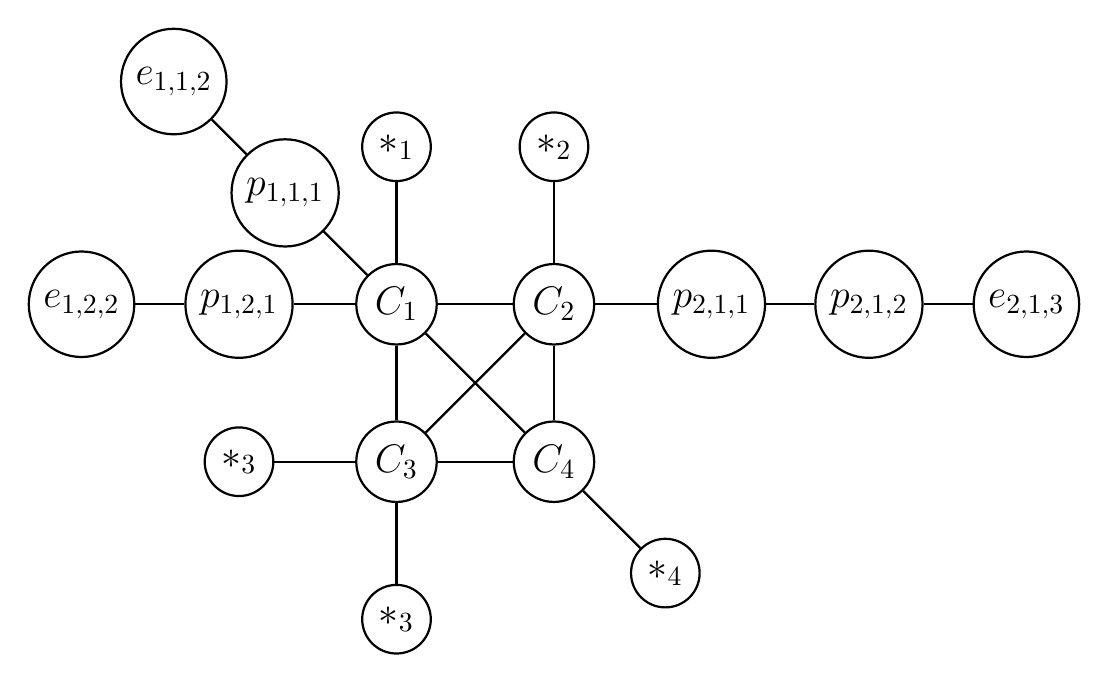
\begin{tikzpicture}[-,auto,node distance=2cm,
                    thick,main node/.style={circle,draw,font=\sffamily\Large\bfseries}]

 \node[main node] (c1) {$C_{1}$};
 \node[main node] (1) [above of=c1] {$*_{1}$};
 \node[main node] (2) [above left of=c1] {$p_{1,1,1}$};
 \node[main node] (3) [left of=c1] {$p_{1,2,1}$};
 \node[main node] (4) [above left of=2] {$e_{1,1,2}$};
 \node[main node] (5) [left of=3] {$e_{1,2,2}$};
  
 \path
 (c1) edge (1)
      edge (2)
      edge (3)
  (2) edge (4)
  (3) edge (5);
 
 \node[main node] (c2) [right of=c1] {$C_{2}$};
 \node[main node] (6) [above of=c2] {$*_{2}$};
 \node[main node] (7) [right of=c2] {$p_{2,1,1}$};
 \node[main node] (8) [right of=7] {$p_{2,1,2}$};
 \node[main node] (9) [right of=8] {$e_{2,1,3}$};
 
  \path
 (c2) edge (6)
      edge (7)
  (7) edge (8)
  (8) edge (9);
      
 \node[main node] (c3) [below of=c1] {$C_{3}$};
 \node[main node] (10) [below of=c3] {$*_{3}$};
 \node[main node] (11) [left of=c3] {$*_{3}$};
 
  \path
 (c3) edge (10)
      edge (11);
      
 \node[main node] (c4) [below of=c2] {$C_{4}$};
 \node[main node] (12) [below right of=c4] {$*_{4}$};
 
  \path
 (c4) edge (12);            
  
 \path
 (c1) edge (c2)
      edge (c3)
      edge (c4)
 (c2) edge (c3)
      edge (c4)
 (c3) edge (c4);
 
        
  
\end{tikzpicture}
\end{center}
\caption{Example of labelling on $(S_{3}^{1,1},S_{2}^{2},S_{2},S_{1})$.}
\label{myfigure: Example of labeling on multi general star graph}
\end{myfigure}

Because we have just joined graphs we know some solutions to, we can use decomposition for the patrollers strategy, and simplification for the attackers strategy.

\begin{theorem}[Separable solution]
\

For $ 2(K_{\text{max}}+1) \leq m \leq 2 \min\limits_{i=1,...,p} \{n_{i}+\sum\limits_{j=1}^{h_{i}} (\bm{k}_{i})_{j} \}$,

\begin{align*}
V = \frac{m}{2 \sum\limits_{i=1}^{p} \left(n_{i}+\sum\limits_{j=1}^{h_{i}} (\bm{k}_{i})_{j}\right)}
\equiv \frac{m}{2(|\bm{n}|+|\bm{K}|)}
\end{align*}
where $\bm{K}$ is the concatenation of all the $\bm{k}_{i}$ vectors for $i=1,...,p$, with $K_{\text{max}}=\max{\bm{K}}$ and $\bm{n}=(n_{1},...,n_{p})$.
\end{theorem}

\begin{proof}
Under decomposition with the Hamiltonian bound for the general star graphs, as $m \leq 2 \min\limits_{i=1,...,p} \{n_{i}+\sum\limits_{j=1}^{h_{i}} (\bm{k}_{i})_{j} \}$
 
$$V \geq \frac{1}{\sum\limits_{i=1}^{k} \frac{2(n_{i}+|\bm{k}_{i}|)}{m}}=\frac{m}{2 \sum\limits_{i=1}^{k} (n_{i}+|\bm{k}_{i}|)}$$

Now under simplification of the centre's, i.e $\bigodot\limits_{i=1}^{p} S_{n_{i}}^{\bm{k}_{i}}$ to $S_{|\bm{n}|}^{\bm{K}}$, as $m \geq 2(K_{\text{max}}+1)$

$$V \leq \frac{m}{2( |\bm{n}| + |\bm{K}|)}$$

So we have a tight upper and lower bound.
\end{proof}



\begin{myfigure}
\begin{center}
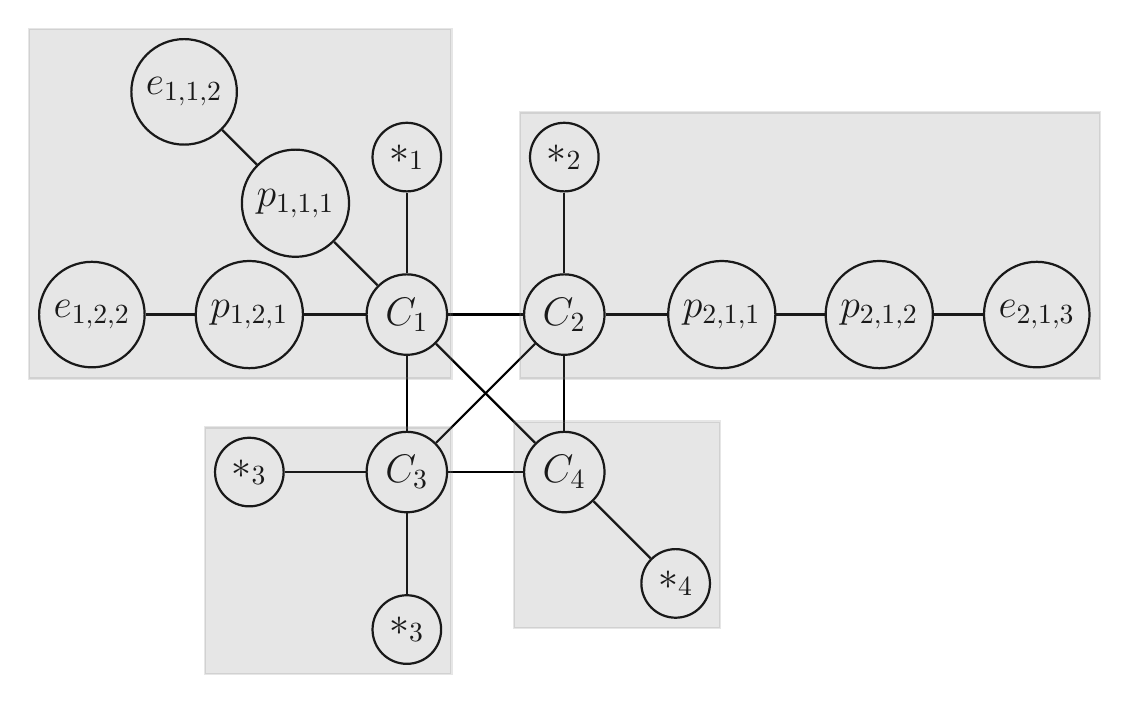
\begin{tikzpicture}[-,auto,node distance=2cm,
                    thick,main node/.style={circle,draw,font=\sffamily\Large\bfseries}]

 \node[main node] (c1) {$C_{1}$};
 \node[main node] (1) [above of=c1] {$*_{1}$};
 \node[main node] (2) [above left of=c1] {$p_{1,1,1}$};
 \node[main node] (3) [left of=c1] {$p_{1,2,1}$};
 \node[main node] (4) [above left of=2] {$e_{1,1,2}$};
 \node[main node] (5) [left of=3] {$e_{1,2,2}$};
  
 \path
 (c1) edge (1)
      edge (2)
      edge (3)
  (2) edge (4)
  (3) edge (5);
 
 \node[main node] (c2) [right of=c1] {$C_{2}$};
 \node[main node] (6) [above of=c2] {$*_{2}$};
 \node[main node] (7) [right of=c2] {$p_{2,1,1}$};
 \node[main node] (8) [right of=7] {$p_{2,1,2}$};
 \node[main node] (9) [right of=8] {$e_{2,1,3}$};
 
  \path
 (c2) edge (6)
      edge (7)
  (7) edge (8)
  (8) edge (9);
      
 \node[main node] (c3) [below of=c1] {$C_{3}$};
 \node[main node] (10) [below of=c3] {$*_{3}$};
 \node[main node] (11) [left of=c3] {$*_{3}$};
 
  \path
 (c3) edge (10)
      edge (11);
      
 \node[main node] (c4) [below of=c2] {$C_{4}$};
 \node[main node] (12) [below right of=c4] {$*_{4}$};
 
  \path
 (c4) edge (12);            
  
 \path
 (c1) edge (c2)
      edge (c3)
      edge (c4)
 (c2) edge (c3)
      edge (c4)
 (c3) edge (c4);  
 
   \node (Box1) [draw,thick,fit=(1) (2) (3) (4) (5),fill,gray,opacity=0.2] {};
   
      \node (Box2) [draw,thick,fit=(6) (7) (8) (9),fill,gray,opacity=0.2] {};
      
         \node (Box3) [draw,thick,fit=(10) (11),fill,gray,opacity=0.2] {};
         
            \node (Box4) [draw,thick,fit=(c4) (12),fill,gray,opacity=0.2] {};
        
  
\end{tikzpicture}
\end{center}
\caption{Example of decomposition on $(S_{3}^{1,1},S_{2}^{2},S_{2},S_{1})$.}
\label{myfigure: Example of decomposition on multi general star graph}
\end{myfigure}


\begin{myfigure}
\begin{center}
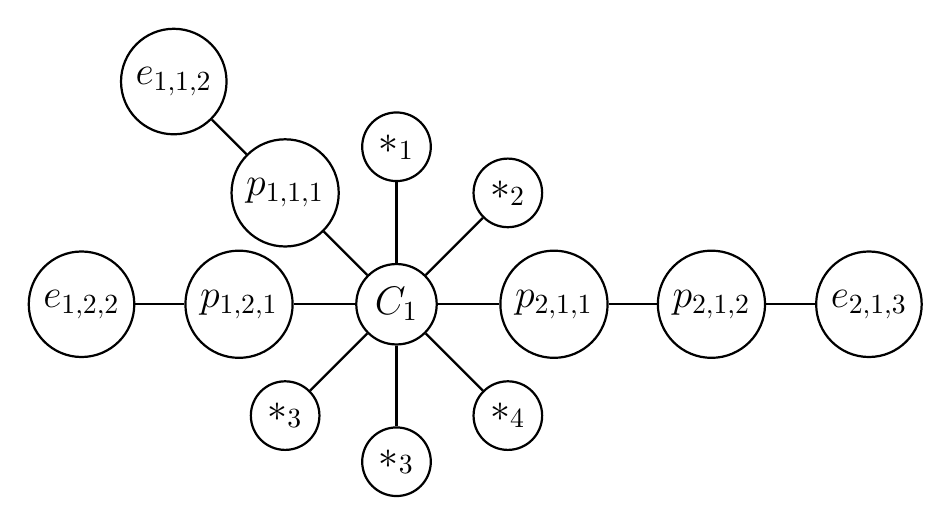
\begin{tikzpicture}[-,auto,node distance=2cm,
                    thick,main node/.style={circle,draw,font=\sffamily\Large\bfseries}]

 \node[main node] (c1) {$C_{1}$};
 \node[main node] (1) [above of=c1] {$*_{1}$};
 \node[main node] (2) [above left of=c1] {$p_{1,1,1}$};
 \node[main node] (3) [left of=c1] {$p_{1,2,1}$};
 \node[main node] (4) [above left of=2] {$e_{1,1,2}$};
 \node[main node] (5) [left of=3] {$e_{1,2,2}$};
  
 \path
 (c1) edge (1)
      edge (2)
      edge (3)
  (2) edge (4)
  (3) edge (5);
 
 \node[main node] (6) [above right of=c1] {$*_{2}$};
 \node[main node] (7) [right of=c1] {$p_{2,1,1}$};
 \node[main node] (8) [right of=7] {$p_{2,1,2}$};
 \node[main node] (9) [right of=8] {$e_{2,1,3}$};
 
  \path
 (c1) edge (6)
      edge (7)
  (7) edge (8)
  (8) edge (9);
      
 \node[main node] (10) [below of=c1] {$*_{3}$};
 \node[main node] (11) [below left of=c1] {$*_{3}$};
 
  \path
 (c1) edge (10)
      edge (11);
      
 \node[main node] (12) [below right of=c1] {$*_{4}$};
 
  \path
 (c1) edge (12);            
 
  
\end{tikzpicture}
\end{center}
\caption{Example of simplification on $(S_{3}^{1,1},S_{2}^{2},S_{2},S_{1})$ to $S_{8}^{2,1,1}$.}
\label{myfigure: Example of simplification on multi general star graph}
\end{myfigure}

\begin{note}
We note that this is not the Hamiltonian bound for such a graph and the Hamiltonian bound would be,
$$V=\frac{m}{2(|\bm{n}|+|\bm{K}|) + p}$$
\end{note}

\begin{note}
The idea of requiring the complete graph of connection between centres is not needed for the separable solution.
\end{note}


%\section{Strategic Patroller with Random Attackers}
%\label{Section:Strategic Patroller with Random Attackers}
%In this section we provide further work developed from the literature review in Section \ref{Section:Review of patrolling problem with random attackers}.
%
%\subsection{Deterministic Attack time experiments}
%As the theory  works for all bounded attack time distributions, we shall look at the deterministic attack time, using $P(X_{j}=x_{j})=1$, we can note that this does some level of reduction on the state space as costs are only incurred at states with $s_{j}=B_{j}$ or $B_{j}+1$. The cost function reduces to
%
%\begin{align*}
%C_{j}(\bm{s},i)=\begin{cases}
%c_{j} \lambda_{j} R_{j}  \text{ for } s_{j}=B_{j},i \neq j \\ 
%c_{j} \lambda_{j} \text{ for } s_{j}=B_{j}+1,i \neq j  \\
%0 \text{ Otherwise} \\
%\end{cases}
%\end{align*}
%
%and the index reflects this, only wanting the patroller to visit in state, $s=B$, initially and in $s=B+1$ for a higher cost.
%
%\begin{align*}
%W_{j}(\bm{s})=\begin{cases}
%c_{j} \lambda_{j} (B_{j}-1) R_{j}  \text{ for } s_{j}=B_{j}-1 \\ 
%c_{j} \lambda_{j} x_{j} \text{ for } s_{j}=B_{j},B_{j}+1  \\
%0 \text{ Otherwise} \\
%\end{cases}
%\end{align*}
%
%Looking at the single node problem, we notice that there is no cost to transition to the state $s=B$, at which point we incur a cost of $c \lambda R$ to go to $s=B+1$ and then we incur a cost of $c \lambda$.
%
%We notice that the index has its first value in the state $s=B-1$, so in our main problem, when deciding between nodes, we put an index on a state that isn't immediately about to incur cost. Then once its incurring costs, we place a higher index.
%
%However consider a large such as $B=100$ , then for states $s=1,....,98$ we have no index and have no incentive to go visit at all, whether this spike in the index causes any issue with the proposed heuristics is worth some consideration.
%
%\begin{myfigure}
%\begin{center}
%%THIS FIGURE NEEDS REPLOTTING AT SOME POINT (WITH DIFF COSTS)
%% Created by tikzDevice version 0.10.1 on 2018-06-19 09:38:51
% !TEX encoding = UTF-8 Unicode
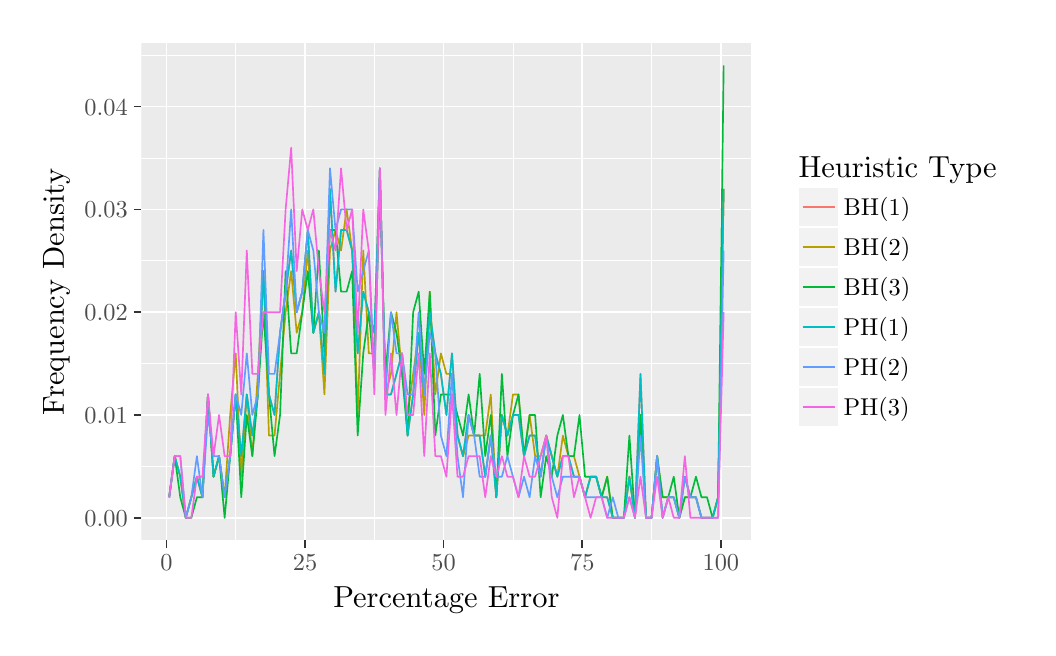
\begin{tikzpicture}[x=1pt,y=1pt]
\definecolor{fillColor}{RGB}{255,255,255}
\path[use as bounding box,fill=fillColor,fill opacity=0.00] (0,0) rectangle (361.35,216.81);
\begin{scope}
\path[clip] (  0.00,  0.00) rectangle (361.35,216.81);
\definecolor{drawColor}{RGB}{255,255,255}
\definecolor{fillColor}{RGB}{255,255,255}

\path[draw=drawColor,line width= 0.6pt,line join=round,line cap=round,fill=fillColor] (  0.00,  0.00) rectangle (361.35,216.81);
\end{scope}
\begin{scope}
\path[clip] ( 41.11, 31.53) rectangle (261.51,211.31);
\definecolor{fillColor}{gray}{0.92}

\path[fill=fillColor] ( 41.11, 31.53) rectangle (261.51,211.31);
\definecolor{drawColor}{RGB}{255,255,255}

\path[draw=drawColor,line width= 0.3pt,line join=round] ( 41.11, 58.27) --
	(261.51, 58.27);

\path[draw=drawColor,line width= 0.3pt,line join=round] ( 41.11, 95.42) --
	(261.51, 95.42);

\path[draw=drawColor,line width= 0.3pt,line join=round] ( 41.11,132.56) --
	(261.51,132.56);

\path[draw=drawColor,line width= 0.3pt,line join=round] ( 41.11,169.71) --
	(261.51,169.71);

\path[draw=drawColor,line width= 0.3pt,line join=round] ( 41.11,206.85) --
	(261.51,206.85);

\path[draw=drawColor,line width= 0.3pt,line join=round] ( 75.17, 31.53) --
	( 75.17,211.31);

\path[draw=drawColor,line width= 0.3pt,line join=round] (125.26, 31.53) --
	(125.26,211.31);

\path[draw=drawColor,line width= 0.3pt,line join=round] (175.36, 31.53) --
	(175.36,211.31);

\path[draw=drawColor,line width= 0.3pt,line join=round] (225.45, 31.53) --
	(225.45,211.31);

\path[draw=drawColor,line width= 0.6pt,line join=round] ( 41.11, 39.70) --
	(261.51, 39.70);

\path[draw=drawColor,line width= 0.6pt,line join=round] ( 41.11, 76.85) --
	(261.51, 76.85);

\path[draw=drawColor,line width= 0.6pt,line join=round] ( 41.11,113.99) --
	(261.51,113.99);

\path[draw=drawColor,line width= 0.6pt,line join=round] ( 41.11,151.14) --
	(261.51,151.14);

\path[draw=drawColor,line width= 0.6pt,line join=round] ( 41.11,188.28) --
	(261.51,188.28);

\path[draw=drawColor,line width= 0.6pt,line join=round] ( 50.13, 31.53) --
	( 50.13,211.31);

\path[draw=drawColor,line width= 0.6pt,line join=round] (100.22, 31.53) --
	(100.22,211.31);

\path[draw=drawColor,line width= 0.6pt,line join=round] (150.31, 31.53) --
	(150.31,211.31);

\path[draw=drawColor,line width= 0.6pt,line join=round] (200.40, 31.53) --
	(200.40,211.31);

\path[draw=drawColor,line width= 0.6pt,line join=round] (250.49, 31.53) --
	(250.49,211.31);
\definecolor{drawColor}{RGB}{248,118,109}

\path[draw=drawColor,line width= 0.6pt,line join=round] ( 51.13, 47.13) --
	( 53.13, 61.99) --
	( 55.14, 54.56) --
	( 57.14, 39.70) --
	( 59.14, 47.13) --
	( 61.15, 54.56) --
	( 63.15, 47.13) --
	( 65.15, 84.28) --
	( 67.16, 54.56) --
	( 69.16, 61.99) --
	( 71.17, 47.13) --
	( 73.17, 61.99) --
	( 75.17, 84.28) --
	( 77.18, 61.99) --
	( 79.18, 84.28) --
	( 81.18, 69.42) --
	( 83.19, 84.28) --
	( 85.19,128.85) --
	( 87.19, 84.28) --
	( 89.20, 76.85) --
	( 91.20,106.56) --
	( 93.21,121.42) --
	( 95.21,136.28) --
	( 97.21,113.99) --
	( 99.22,121.42) --
	(101.22,143.71) --
	(103.22,106.56) --
	(105.23,113.99) --
	(107.23, 91.70) --
	(109.24,158.56) --
	(111.24,121.42) --
	(113.24,143.71) --
	(115.25,143.71) --
	(117.25,136.28) --
	(119.25, 99.13) --
	(121.26,121.42) --
	(123.26,113.99) --
	(125.26,106.56) --
	(127.27,165.99) --
	(129.27, 84.28) --
	(131.28, 84.28) --
	(133.28, 91.70) --
	(135.28, 99.13) --
	(137.29, 69.42) --
	(139.29, 84.28) --
	(141.29,106.56) --
	(143.30, 84.28) --
	(145.30,113.99) --
	(147.30, 99.13) --
	(149.31, 91.70) --
	(151.31, 76.85) --
	(153.32, 99.13) --
	(155.32, 69.42) --
	(157.32, 61.99) --
	(159.33, 76.85) --
	(161.33, 69.42) --
	(163.33, 69.42) --
	(165.34, 54.56) --
	(167.34, 69.42) --
	(169.34, 47.13) --
	(171.35, 76.85) --
	(173.35, 69.42) --
	(175.36, 76.85) --
	(177.36, 76.85) --
	(179.36, 61.99) --
	(181.37, 69.42) --
	(183.37, 69.42) --
	(185.37, 54.56) --
	(187.38, 69.42) --
	(189.38, 61.99) --
	(191.39, 54.56) --
	(193.39, 61.99) --
	(195.39, 61.99) --
	(197.40, 54.56) --
	(199.40, 54.56) --
	(201.40, 47.13) --
	(203.41, 54.56) --
	(205.41, 54.56) --
	(207.41, 47.13) --
	(209.42, 47.13) --
	(211.42, 39.70) --
	(213.43, 39.70) --
	(215.43, 39.70) --
	(217.43, 54.56) --
	(219.44, 39.70) --
	(221.44, 91.70) --
	(223.44, 39.70) --
	(225.45, 39.70) --
	(227.45, 61.99) --
	(229.45, 39.70) --
	(231.46, 47.13) --
	(233.46, 47.13) --
	(235.47, 39.70) --
	(237.47, 54.56) --
	(239.47, 47.13) --
	(241.48, 47.13) --
	(243.48, 39.70) --
	(245.48, 39.70) --
	(247.49, 39.70) --
	(249.49, 47.13) --
	(251.49,158.56);
\definecolor{drawColor}{RGB}{183,159,0}

\path[draw=drawColor,line width= 0.6pt,line join=round] ( 51.13, 47.13) --
	( 53.13, 61.99) --
	( 55.14, 54.56) --
	( 57.14, 39.70) --
	( 59.14, 47.13) --
	( 61.15, 54.56) --
	( 63.15, 47.13) --
	( 65.15, 84.28) --
	( 67.16, 54.56) --
	( 69.16, 61.99) --
	( 71.17, 47.13) --
	( 73.17, 76.85) --
	( 75.17, 99.13) --
	( 77.18, 54.56) --
	( 79.18, 84.28) --
	( 81.18, 61.99) --
	( 83.19, 91.70) --
	( 85.19,128.85) --
	( 87.19, 69.42) --
	( 89.20, 69.42) --
	( 91.20, 91.70) --
	( 93.21,113.99) --
	( 95.21,128.85) --
	( 97.21,106.56) --
	( 99.22,113.99) --
	(101.22,136.28) --
	(103.22,106.56) --
	(105.23,113.99) --
	(107.23, 84.28) --
	(109.24,136.28) --
	(111.24,143.71) --
	(113.24,136.28) --
	(115.25,151.14) --
	(117.25,136.28) --
	(119.25, 76.85) --
	(121.26,136.28) --
	(123.26, 99.13) --
	(125.26, 99.13) --
	(127.27,165.99) --
	(129.27, 84.28) --
	(131.28, 91.70) --
	(133.28,113.99) --
	(135.28, 91.70) --
	(137.29, 76.85) --
	(139.29, 91.70) --
	(141.29,106.56) --
	(143.30, 76.85) --
	(145.30,121.42) --
	(147.30, 84.28) --
	(149.31, 99.13) --
	(151.31, 91.70) --
	(153.32, 91.70) --
	(155.32, 69.42) --
	(157.32, 61.99) --
	(159.33, 69.42) --
	(161.33, 69.42) --
	(163.33, 69.42) --
	(165.34, 69.42) --
	(167.34, 84.28) --
	(169.34, 47.13) --
	(171.35, 76.85) --
	(173.35, 69.42) --
	(175.36, 84.28) --
	(177.36, 84.28) --
	(179.36, 61.99) --
	(181.37, 76.85) --
	(183.37, 61.99) --
	(185.37, 61.99) --
	(187.38, 69.42) --
	(189.38, 61.99) --
	(191.39, 54.56) --
	(193.39, 69.42) --
	(195.39, 61.99) --
	(197.40, 61.99) --
	(199.40, 54.56) --
	(201.40, 47.13) --
	(203.41, 54.56) --
	(205.41, 54.56) --
	(207.41, 47.13) --
	(209.42, 54.56) --
	(211.42, 39.70) --
	(213.43, 39.70) --
	(215.43, 39.70) --
	(217.43, 54.56) --
	(219.44, 39.70) --
	(221.44, 76.85) --
	(223.44, 39.70) --
	(225.45, 39.70) --
	(227.45, 61.99) --
	(229.45, 47.13) --
	(231.46, 47.13) --
	(233.46, 47.13) --
	(235.47, 39.70) --
	(237.47, 47.13) --
	(239.47, 47.13) --
	(241.48, 47.13) --
	(243.48, 39.70) --
	(245.48, 39.70) --
	(247.49, 39.70) --
	(249.49, 47.13) --
	(251.49,158.56);
\definecolor{drawColor}{RGB}{0,186,56}

\path[draw=drawColor,line width= 0.6pt,line join=round] ( 51.13, 47.13) --
	( 53.13, 61.99) --
	( 55.14, 47.13) --
	( 57.14, 39.70) --
	( 59.14, 39.70) --
	( 61.15, 47.13) --
	( 63.15, 47.13) --
	( 65.15, 84.28) --
	( 67.16, 54.56) --
	( 69.16, 61.99) --
	( 71.17, 39.70) --
	( 73.17, 61.99) --
	( 75.17, 84.28) --
	( 77.18, 47.13) --
	( 79.18, 76.85) --
	( 81.18, 61.99) --
	( 83.19, 84.28) --
	( 85.19,113.99) --
	( 87.19, 84.28) --
	( 89.20, 61.99) --
	( 91.20, 76.85) --
	( 93.21,128.85) --
	( 95.21, 99.13) --
	( 97.21, 99.13) --
	( 99.22,113.99) --
	(101.22,128.85) --
	(103.22,106.56) --
	(105.23,136.28) --
	(107.23, 99.13) --
	(109.24,143.71) --
	(111.24,143.71) --
	(113.24,121.42) --
	(115.25,121.42) --
	(117.25,128.85) --
	(119.25, 69.42) --
	(121.26, 99.13) --
	(123.26,113.99) --
	(125.26, 91.70) --
	(127.27,158.56) --
	(129.27, 91.70) --
	(131.28,113.99) --
	(133.28,106.56) --
	(135.28, 91.70) --
	(137.29, 69.42) --
	(139.29,113.99) --
	(141.29,121.42) --
	(143.30, 91.70) --
	(145.30,121.42) --
	(147.30, 69.42) --
	(149.31, 84.28) --
	(151.31, 84.28) --
	(153.32, 84.28) --
	(155.32, 76.85) --
	(157.32, 69.42) --
	(159.33, 84.28) --
	(161.33, 69.42) --
	(163.33, 91.70) --
	(165.34, 61.99) --
	(167.34, 76.85) --
	(169.34, 47.13) --
	(171.35, 91.70) --
	(173.35, 61.99) --
	(175.36, 76.85) --
	(177.36, 84.28) --
	(179.36, 61.99) --
	(181.37, 76.85) --
	(183.37, 76.85) --
	(185.37, 47.13) --
	(187.38, 61.99) --
	(189.38, 54.56) --
	(191.39, 69.42) --
	(193.39, 76.85) --
	(195.39, 61.99) --
	(197.40, 61.99) --
	(199.40, 76.85) --
	(201.40, 54.56) --
	(203.41, 54.56) --
	(205.41, 54.56) --
	(207.41, 47.13) --
	(209.42, 54.56) --
	(211.42, 39.70) --
	(213.43, 39.70) --
	(215.43, 39.70) --
	(217.43, 69.42) --
	(219.44, 39.70) --
	(221.44, 76.85) --
	(223.44, 39.70) --
	(225.45, 39.70) --
	(227.45, 61.99) --
	(229.45, 47.13) --
	(231.46, 47.13) --
	(233.46, 54.56) --
	(235.47, 39.70) --
	(237.47, 47.13) --
	(239.47, 47.13) --
	(241.48, 54.56) --
	(243.48, 47.13) --
	(245.48, 47.13) --
	(247.49, 39.70) --
	(249.49, 47.13) --
	(251.49,203.14);
\definecolor{drawColor}{RGB}{0,191,196}

\path[draw=drawColor,line width= 0.6pt,line join=round] ( 51.13, 47.13) --
	( 53.13, 61.99) --
	( 55.14, 54.56) --
	( 57.14, 39.70) --
	( 59.14, 47.13) --
	( 61.15, 54.56) --
	( 63.15, 47.13) --
	( 65.15, 84.28) --
	( 67.16, 54.56) --
	( 69.16, 61.99) --
	( 71.17, 47.13) --
	( 73.17, 61.99) --
	( 75.17, 84.28) --
	( 77.18, 61.99) --
	( 79.18, 84.28) --
	( 81.18, 69.42) --
	( 83.19, 84.28) --
	( 85.19,128.85) --
	( 87.19, 84.28) --
	( 89.20, 76.85) --
	( 91.20,106.56) --
	( 93.21,121.42) --
	( 95.21,136.28) --
	( 97.21,113.99) --
	( 99.22,121.42) --
	(101.22,143.71) --
	(103.22,106.56) --
	(105.23,113.99) --
	(107.23, 91.70) --
	(109.24,158.56) --
	(111.24,121.42) --
	(113.24,143.71) --
	(115.25,143.71) --
	(117.25,136.28) --
	(119.25, 99.13) --
	(121.26,121.42) --
	(123.26,113.99) --
	(125.26,106.56) --
	(127.27,165.99) --
	(129.27, 84.28) --
	(131.28, 84.28) --
	(133.28, 91.70) --
	(135.28, 99.13) --
	(137.29, 69.42) --
	(139.29, 84.28) --
	(141.29,106.56) --
	(143.30, 84.28) --
	(145.30,113.99) --
	(147.30, 99.13) --
	(149.31, 91.70) --
	(151.31, 76.85) --
	(153.32, 99.13) --
	(155.32, 69.42) --
	(157.32, 61.99) --
	(159.33, 76.85) --
	(161.33, 69.42) --
	(163.33, 69.42) --
	(165.34, 54.56) --
	(167.34, 69.42) --
	(169.34, 47.13) --
	(171.35, 76.85) --
	(173.35, 69.42) --
	(175.36, 76.85) --
	(177.36, 76.85) --
	(179.36, 61.99) --
	(181.37, 69.42) --
	(183.37, 69.42) --
	(185.37, 54.56) --
	(187.38, 69.42) --
	(189.38, 61.99) --
	(191.39, 54.56) --
	(193.39, 61.99) --
	(195.39, 61.99) --
	(197.40, 54.56) --
	(199.40, 54.56) --
	(201.40, 47.13) --
	(203.41, 54.56) --
	(205.41, 54.56) --
	(207.41, 47.13) --
	(209.42, 47.13) --
	(211.42, 39.70) --
	(213.43, 39.70) --
	(215.43, 39.70) --
	(217.43, 54.56) --
	(219.44, 39.70) --
	(221.44, 91.70) --
	(223.44, 39.70) --
	(225.45, 39.70) --
	(227.45, 61.99) --
	(229.45, 39.70) --
	(231.46, 47.13) --
	(233.46, 47.13) --
	(235.47, 39.70) --
	(237.47, 54.56) --
	(239.47, 47.13) --
	(241.48, 47.13) --
	(243.48, 39.70) --
	(245.48, 39.70) --
	(247.49, 39.70) --
	(249.49, 47.13) --
	(251.49,158.56);
\definecolor{drawColor}{RGB}{97,156,255}

\path[draw=drawColor,line width= 0.6pt,line join=round] ( 51.13, 47.13) --
	( 53.13, 61.99) --
	( 55.14, 61.99) --
	( 57.14, 39.70) --
	( 59.14, 47.13) --
	( 61.15, 61.99) --
	( 63.15, 47.13) --
	( 65.15, 76.85) --
	( 67.16, 61.99) --
	( 69.16, 61.99) --
	( 71.17, 47.13) --
	( 73.17, 61.99) --
	( 75.17, 84.28) --
	( 77.18, 76.85) --
	( 79.18, 99.13) --
	( 81.18, 76.85) --
	( 83.19, 84.28) --
	( 85.19,143.71) --
	( 87.19, 91.70) --
	( 89.20, 91.70) --
	( 91.20,106.56) --
	( 93.21,121.42) --
	( 95.21,151.14) --
	( 97.21,113.99) --
	( 99.22,121.42) --
	(101.22,143.71) --
	(103.22,136.28) --
	(105.23,113.99) --
	(107.23,106.56) --
	(109.24,165.99) --
	(111.24,143.71) --
	(113.24,151.14) --
	(115.25,151.14) --
	(117.25,151.14) --
	(119.25,121.42) --
	(121.26,128.85) --
	(123.26,136.28) --
	(125.26, 91.70) --
	(127.27,165.99) --
	(129.27, 84.28) --
	(131.28,113.99) --
	(133.28, 99.13) --
	(135.28, 99.13) --
	(137.29, 84.28) --
	(139.29, 84.28) --
	(141.29,113.99) --
	(143.30, 84.28) --
	(145.30,106.56) --
	(147.30, 99.13) --
	(149.31, 69.42) --
	(151.31, 61.99) --
	(153.32, 91.70) --
	(155.32, 61.99) --
	(157.32, 47.13) --
	(159.33, 76.85) --
	(161.33, 69.42) --
	(163.33, 54.56) --
	(165.34, 54.56) --
	(167.34, 69.42) --
	(169.34, 54.56) --
	(171.35, 54.56) --
	(173.35, 61.99) --
	(175.36, 54.56) --
	(177.36, 47.13) --
	(179.36, 54.56) --
	(181.37, 47.13) --
	(183.37, 61.99) --
	(185.37, 54.56) --
	(187.38, 69.42) --
	(189.38, 54.56) --
	(191.39, 47.13) --
	(193.39, 54.56) --
	(195.39, 54.56) --
	(197.40, 54.56) --
	(199.40, 54.56) --
	(201.40, 47.13) --
	(203.41, 47.13) --
	(205.41, 47.13) --
	(207.41, 47.13) --
	(209.42, 39.70) --
	(211.42, 47.13) --
	(213.43, 39.70) --
	(215.43, 39.70) --
	(217.43, 47.13) --
	(219.44, 39.70) --
	(221.44, 69.42) --
	(223.44, 39.70) --
	(225.45, 39.70) --
	(227.45, 61.99) --
	(229.45, 39.70) --
	(231.46, 47.13) --
	(233.46, 47.13) --
	(235.47, 39.70) --
	(237.47, 54.56) --
	(239.47, 47.13) --
	(241.48, 47.13) --
	(243.48, 39.70) --
	(245.48, 39.70) --
	(247.49, 39.70) --
	(249.49, 39.70) --
	(251.49,136.28);
\definecolor{drawColor}{RGB}{245,100,227}

\path[draw=drawColor,line width= 0.6pt,line join=round] ( 51.13, 47.13) --
	( 53.13, 61.99) --
	( 55.14, 61.99) --
	( 57.14, 39.70) --
	( 59.14, 39.70) --
	( 61.15, 54.56) --
	( 63.15, 54.56) --
	( 65.15, 84.28) --
	( 67.16, 61.99) --
	( 69.16, 76.85) --
	( 71.17, 61.99) --
	( 73.17, 61.99) --
	( 75.17,113.99) --
	( 77.18, 84.28) --
	( 79.18,136.28) --
	( 81.18, 91.70) --
	( 83.19, 91.70) --
	( 85.19,113.99) --
	( 87.19,113.99) --
	( 89.20,113.99) --
	( 91.20,113.99) --
	( 93.21,151.14) --
	( 95.21,173.42) --
	( 97.21,128.85) --
	( 99.22,151.14) --
	(101.22,143.71) --
	(103.22,151.14) --
	(105.23,128.85) --
	(107.23,113.99) --
	(109.24,143.71) --
	(111.24,136.28) --
	(113.24,165.99) --
	(115.25,143.71) --
	(117.25,151.14) --
	(119.25,106.56) --
	(121.26,151.14) --
	(123.26,136.28) --
	(125.26, 84.28) --
	(127.27,165.99) --
	(129.27, 76.85) --
	(131.28, 99.13) --
	(133.28, 76.85) --
	(135.28, 99.13) --
	(137.29, 76.85) --
	(139.29, 76.85) --
	(141.29, 99.13) --
	(143.30, 61.99) --
	(145.30, 99.13) --
	(147.30, 61.99) --
	(149.31, 61.99) --
	(151.31, 54.56) --
	(153.32, 84.28) --
	(155.32, 54.56) --
	(157.32, 54.56) --
	(159.33, 61.99) --
	(161.33, 61.99) --
	(163.33, 61.99) --
	(165.34, 47.13) --
	(167.34, 61.99) --
	(169.34, 54.56) --
	(171.35, 61.99) --
	(173.35, 54.56) --
	(175.36, 54.56) --
	(177.36, 47.13) --
	(179.36, 61.99) --
	(181.37, 54.56) --
	(183.37, 54.56) --
	(185.37, 61.99) --
	(187.38, 69.42) --
	(189.38, 47.13) --
	(191.39, 39.70) --
	(193.39, 61.99) --
	(195.39, 61.99) --
	(197.40, 47.13) --
	(199.40, 54.56) --
	(201.40, 47.13) --
	(203.41, 39.70) --
	(205.41, 47.13) --
	(207.41, 47.13) --
	(209.42, 39.70) --
	(211.42, 39.70) --
	(213.43, 39.70) --
	(215.43, 39.70) --
	(217.43, 47.13) --
	(219.44, 39.70) --
	(221.44, 54.56) --
	(223.44, 39.70) --
	(225.45, 39.70) --
	(227.45, 54.56) --
	(229.45, 39.70) --
	(231.46, 47.13) --
	(233.46, 39.70) --
	(235.47, 39.70) --
	(237.47, 61.99) --
	(239.47, 39.70) --
	(241.48, 39.70) --
	(243.48, 39.70) --
	(245.48, 39.70) --
	(247.49, 39.70) --
	(249.49, 39.70) --
	(251.49,113.99);
\end{scope}
\begin{scope}
\path[clip] (  0.00,  0.00) rectangle (361.35,216.81);
\definecolor{drawColor}{gray}{0.30}

\node[text=drawColor,anchor=base east,inner sep=0pt, outer sep=0pt, scale=  0.88] at ( 36.16, 36.67) {0.00};

\node[text=drawColor,anchor=base east,inner sep=0pt, outer sep=0pt, scale=  0.88] at ( 36.16, 73.82) {0.01};

\node[text=drawColor,anchor=base east,inner sep=0pt, outer sep=0pt, scale=  0.88] at ( 36.16,110.96) {0.02};

\node[text=drawColor,anchor=base east,inner sep=0pt, outer sep=0pt, scale=  0.88] at ( 36.16,148.11) {0.03};

\node[text=drawColor,anchor=base east,inner sep=0pt, outer sep=0pt, scale=  0.88] at ( 36.16,185.25) {0.04};
\end{scope}
\begin{scope}
\path[clip] (  0.00,  0.00) rectangle (361.35,216.81);
\definecolor{drawColor}{gray}{0.20}

\path[draw=drawColor,line width= 0.6pt,line join=round] ( 38.36, 39.70) --
	( 41.11, 39.70);

\path[draw=drawColor,line width= 0.6pt,line join=round] ( 38.36, 76.85) --
	( 41.11, 76.85);

\path[draw=drawColor,line width= 0.6pt,line join=round] ( 38.36,113.99) --
	( 41.11,113.99);

\path[draw=drawColor,line width= 0.6pt,line join=round] ( 38.36,151.14) --
	( 41.11,151.14);

\path[draw=drawColor,line width= 0.6pt,line join=round] ( 38.36,188.28) --
	( 41.11,188.28);
\end{scope}
\begin{scope}
\path[clip] (  0.00,  0.00) rectangle (361.35,216.81);
\definecolor{drawColor}{gray}{0.20}

\path[draw=drawColor,line width= 0.6pt,line join=round] ( 50.13, 28.78) --
	( 50.13, 31.53);

\path[draw=drawColor,line width= 0.6pt,line join=round] (100.22, 28.78) --
	(100.22, 31.53);

\path[draw=drawColor,line width= 0.6pt,line join=round] (150.31, 28.78) --
	(150.31, 31.53);

\path[draw=drawColor,line width= 0.6pt,line join=round] (200.40, 28.78) --
	(200.40, 31.53);

\path[draw=drawColor,line width= 0.6pt,line join=round] (250.49, 28.78) --
	(250.49, 31.53);
\end{scope}
\begin{scope}
\path[clip] (  0.00,  0.00) rectangle (361.35,216.81);
\definecolor{drawColor}{gray}{0.30}

\node[text=drawColor,anchor=base,inner sep=0pt, outer sep=0pt, scale=  0.88] at ( 50.13, 20.52) {0};

\node[text=drawColor,anchor=base,inner sep=0pt, outer sep=0pt, scale=  0.88] at (100.22, 20.52) {25};

\node[text=drawColor,anchor=base,inner sep=0pt, outer sep=0pt, scale=  0.88] at (150.31, 20.52) {50};

\node[text=drawColor,anchor=base,inner sep=0pt, outer sep=0pt, scale=  0.88] at (200.40, 20.52) {75};

\node[text=drawColor,anchor=base,inner sep=0pt, outer sep=0pt, scale=  0.88] at (250.49, 20.52) {100};
\end{scope}
\begin{scope}
\path[clip] (  0.00,  0.00) rectangle (361.35,216.81);
\definecolor{drawColor}{RGB}{0,0,0}

\node[text=drawColor,anchor=base,inner sep=0pt, outer sep=0pt, scale=  1.10] at (151.31,  7.44) {Percentage Error};
\end{scope}
\begin{scope}
\path[clip] (  0.00,  0.00) rectangle (361.35,216.81);
\definecolor{drawColor}{RGB}{0,0,0}

\node[text=drawColor,rotate= 90.00,anchor=base,inner sep=0pt, outer sep=0pt, scale=  1.10] at ( 13.08,121.42) {Frequency Density};
\end{scope}
\begin{scope}
\path[clip] (  0.00,  0.00) rectangle (361.35,216.81);
\definecolor{fillColor}{RGB}{255,255,255}

\path[fill=fillColor] (272.89, 66.77) rectangle (355.85,176.07);
\end{scope}
\begin{scope}
\path[clip] (  0.00,  0.00) rectangle (361.35,216.81);
\definecolor{drawColor}{RGB}{0,0,0}

\node[text=drawColor,anchor=base west,inner sep=0pt, outer sep=0pt, scale=  1.10] at (278.58,162.80) {Heuristic Type};
\end{scope}
\begin{scope}
\path[clip] (  0.00,  0.00) rectangle (361.35,216.81);
\definecolor{drawColor}{RGB}{255,255,255}
\definecolor{fillColor}{gray}{0.95}

\path[draw=drawColor,line width= 0.6pt,line join=round,line cap=round,fill=fillColor] (278.58,144.73) rectangle (293.04,159.19);
\end{scope}
\begin{scope}
\path[clip] (  0.00,  0.00) rectangle (361.35,216.81);
\definecolor{drawColor}{RGB}{248,118,109}

\path[draw=drawColor,line width= 0.6pt,line join=round] (280.03,151.96) -- (291.59,151.96);
\end{scope}
\begin{scope}
\path[clip] (  0.00,  0.00) rectangle (361.35,216.81);
\definecolor{drawColor}{RGB}{255,255,255}
\definecolor{fillColor}{gray}{0.95}

\path[draw=drawColor,line width= 0.6pt,line join=round,line cap=round,fill=fillColor] (278.58,130.28) rectangle (293.04,144.73);
\end{scope}
\begin{scope}
\path[clip] (  0.00,  0.00) rectangle (361.35,216.81);
\definecolor{drawColor}{RGB}{183,159,0}

\path[draw=drawColor,line width= 0.6pt,line join=round] (280.03,137.51) -- (291.59,137.51);
\end{scope}
\begin{scope}
\path[clip] (  0.00,  0.00) rectangle (361.35,216.81);
\definecolor{drawColor}{RGB}{255,255,255}
\definecolor{fillColor}{gray}{0.95}

\path[draw=drawColor,line width= 0.6pt,line join=round,line cap=round,fill=fillColor] (278.58,115.83) rectangle (293.04,130.28);
\end{scope}
\begin{scope}
\path[clip] (  0.00,  0.00) rectangle (361.35,216.81);
\definecolor{drawColor}{RGB}{0,186,56}

\path[draw=drawColor,line width= 0.6pt,line join=round] (280.03,123.05) -- (291.59,123.05);
\end{scope}
\begin{scope}
\path[clip] (  0.00,  0.00) rectangle (361.35,216.81);
\definecolor{drawColor}{RGB}{255,255,255}
\definecolor{fillColor}{gray}{0.95}

\path[draw=drawColor,line width= 0.6pt,line join=round,line cap=round,fill=fillColor] (278.58,101.37) rectangle (293.04,115.83);
\end{scope}
\begin{scope}
\path[clip] (  0.00,  0.00) rectangle (361.35,216.81);
\definecolor{drawColor}{RGB}{0,191,196}

\path[draw=drawColor,line width= 0.6pt,line join=round] (280.03,108.60) -- (291.59,108.60);
\end{scope}
\begin{scope}
\path[clip] (  0.00,  0.00) rectangle (361.35,216.81);
\definecolor{drawColor}{RGB}{255,255,255}
\definecolor{fillColor}{gray}{0.95}

\path[draw=drawColor,line width= 0.6pt,line join=round,line cap=round,fill=fillColor] (278.58, 86.92) rectangle (293.04,101.37);
\end{scope}
\begin{scope}
\path[clip] (  0.00,  0.00) rectangle (361.35,216.81);
\definecolor{drawColor}{RGB}{97,156,255}

\path[draw=drawColor,line width= 0.6pt,line join=round] (280.03, 94.14) -- (291.59, 94.14);
\end{scope}
\begin{scope}
\path[clip] (  0.00,  0.00) rectangle (361.35,216.81);
\definecolor{drawColor}{RGB}{255,255,255}
\definecolor{fillColor}{gray}{0.95}

\path[draw=drawColor,line width= 0.6pt,line join=round,line cap=round,fill=fillColor] (278.58, 72.46) rectangle (293.04, 86.92);
\end{scope}
\begin{scope}
\path[clip] (  0.00,  0.00) rectangle (361.35,216.81);
\definecolor{drawColor}{RGB}{245,100,227}

\path[draw=drawColor,line width= 0.6pt,line join=round] (280.03, 79.69) -- (291.59, 79.69);
\end{scope}
\begin{scope}
\path[clip] (  0.00,  0.00) rectangle (361.35,216.81);
\definecolor{drawColor}{RGB}{0,0,0}

\node[text=drawColor,anchor=base west,inner sep=0pt, outer sep=0pt, scale=  0.88] at (294.85,148.93) {BH($1$)};
\end{scope}
\begin{scope}
\path[clip] (  0.00,  0.00) rectangle (361.35,216.81);
\definecolor{drawColor}{RGB}{0,0,0}

\node[text=drawColor,anchor=base west,inner sep=0pt, outer sep=0pt, scale=  0.88] at (294.85,134.48) {BH($2$)};
\end{scope}
\begin{scope}
\path[clip] (  0.00,  0.00) rectangle (361.35,216.81);
\definecolor{drawColor}{RGB}{0,0,0}

\node[text=drawColor,anchor=base west,inner sep=0pt, outer sep=0pt, scale=  0.88] at (294.85,120.02) {BH($3$)};
\end{scope}
\begin{scope}
\path[clip] (  0.00,  0.00) rectangle (361.35,216.81);
\definecolor{drawColor}{RGB}{0,0,0}

\node[text=drawColor,anchor=base west,inner sep=0pt, outer sep=0pt, scale=  0.88] at (294.85,105.57) {PH($1$)};
\end{scope}
\begin{scope}
\path[clip] (  0.00,  0.00) rectangle (361.35,216.81);
\definecolor{drawColor}{RGB}{0,0,0}

\node[text=drawColor,anchor=base west,inner sep=0pt, outer sep=0pt, scale=  0.88] at (294.85, 91.11) {PH($2$)};
\end{scope}
\begin{scope}
\path[clip] (  0.00,  0.00) rectangle (361.35,216.81);
\definecolor{drawColor}{RGB}{0,0,0}

\node[text=drawColor,anchor=base west,inner sep=0pt, outer sep=0pt, scale=  0.88] at (294.85, 76.66) {PH($3$)};
\end{scope}
\end{tikzpicture}

%\end{center}
%\caption{Frequency of percentage error with only deterministic attack times}
%\label{Figure:Deterministic attack times}
%\end{myfigure}
%
%\subsection{Smoothing the index}
%To smooth the spike in index, we could suggest splitting up the index in some fashion. Before we suggest splitting the index through we must take into consideration how the benefit and penalty heuristics differ. As the penalty is measuring how much index is not claimed, it should be easy to split it amongst all states $s \leq B-1$, so that the sum is the correct index. But the benefit is measuring how much index is claimed, so it needs to be cumulative and is therefore a little harder to split amongst all the states $s \leq B-1$, we do not need that sum is the correct index.
%
%Consider a the splitting function, for node $j$'s index, $l_{j}(x)$ with $x \in [1,....,B_{j}-1]$ s.t $L_{j}(B_{j}-1)=B_{j}-1$ where $L_{j}(x)=\sum\limits_{u=1}^{x} l_{j}(u)$ , and to place more emphasis on the spike we will require that $l_{j}(x)$ is non-decreasing. For now we will assume the same splitting is used on each node, dropping the subscript.
%
%\begin{align*}
%W_{j}^{SP}(\bm{s})=\begin{cases}
%l(s_{j}) \times \frac{c_{j} \lambda R_{j}}{B}  \text{ for } s_{j} \leq B_{j} \\ 
%c_{j} \lambda_{j} \text{ for } s_{j}=B_{j}+1  \\
%\end{cases}
%\end{align*}
%
%and for the benefit use the cumulative version
%
%\begin{align*}
%W_{j}^{SB}(\bm{s})=\begin{cases}
%L(s_{j}) \times \frac{(c_{j} \lambda R_{j})}{B}  \text{ for } s_{j} \leq B_{j} \\ 
%c_{j} \lambda_{j} \text{ for } s_{j}=B_{j}+1  \\
%\end{cases}
%\end{align*}
%
%So the original index has $l(x) =0 \; \forall x \neq B-1$ and $l(B-1)=B-1$. The equal splitting has,$l(x)=1 \; \forall x$. For our numerical study, we will consider using a linear increase $l(x)=\frac{2s_{j}}{B+1} \; \forall x$ for the unequal splitting .
%
%We now present, at depth 3, both the equal and unequal splitting against its original counterpart for the penalty (\ref{Figure:Penalty splitting experiment}) and benefit heuristics (\ref{Figure:Benefit splitting experiment}).
%
%\begin{myfigure}
%%THIS FIGURE NEEDS REPLOTTING AT SOME POINT (WITH DIFF COSTS)
%% Created by tikzDevice version 0.10.1 on 2018-06-21 09:35:15
% !TEX encoding = UTF-8 Unicode
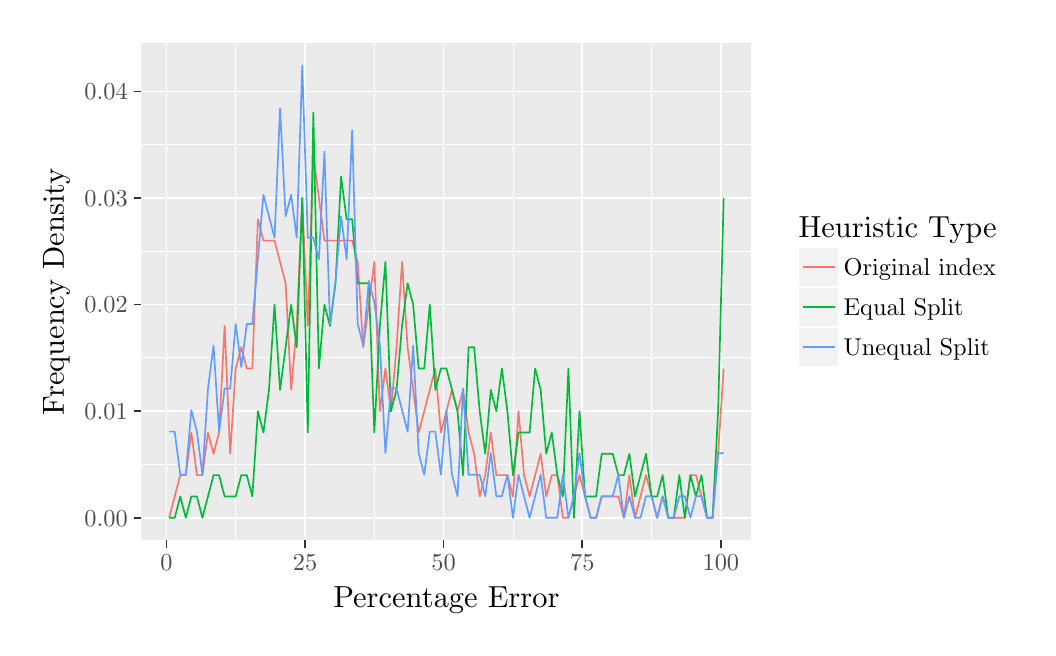
\begin{tikzpicture}[x=1pt,y=1pt]
\definecolor{fillColor}{RGB}{255,255,255}
\path[use as bounding box,fill=fillColor,fill opacity=0.00] (0,0) rectangle (361.35,216.81);
\begin{scope}
\path[clip] (  0.00,  0.00) rectangle (361.35,216.81);
\definecolor{drawColor}{RGB}{255,255,255}
\definecolor{fillColor}{RGB}{255,255,255}

\path[draw=drawColor,line width= 0.6pt,line join=round,line cap=round,fill=fillColor] (  0.00,  0.00) rectangle (361.35,216.81);
\end{scope}
\begin{scope}
\path[clip] ( 41.11, 31.53) rectangle (261.51,211.31);
\definecolor{fillColor}{gray}{0.92}

\path[fill=fillColor] ( 41.11, 31.53) rectangle (261.51,211.31);
\definecolor{drawColor}{RGB}{255,255,255}

\path[draw=drawColor,line width= 0.3pt,line join=round] ( 41.11, 58.96) --
	(261.51, 58.96);

\path[draw=drawColor,line width= 0.3pt,line join=round] ( 41.11, 97.49) --
	(261.51, 97.49);

\path[draw=drawColor,line width= 0.3pt,line join=round] ( 41.11,136.01) --
	(261.51,136.01);

\path[draw=drawColor,line width= 0.3pt,line join=round] ( 41.11,174.54) --
	(261.51,174.54);

\path[draw=drawColor,line width= 0.3pt,line join=round] ( 75.17, 31.53) --
	( 75.17,211.31);

\path[draw=drawColor,line width= 0.3pt,line join=round] (125.26, 31.53) --
	(125.26,211.31);

\path[draw=drawColor,line width= 0.3pt,line join=round] (175.36, 31.53) --
	(175.36,211.31);

\path[draw=drawColor,line width= 0.3pt,line join=round] (225.45, 31.53) --
	(225.45,211.31);

\path[draw=drawColor,line width= 0.6pt,line join=round] ( 41.11, 39.70) --
	(261.51, 39.70);

\path[draw=drawColor,line width= 0.6pt,line join=round] ( 41.11, 78.23) --
	(261.51, 78.23);

\path[draw=drawColor,line width= 0.6pt,line join=round] ( 41.11,116.75) --
	(261.51,116.75);

\path[draw=drawColor,line width= 0.6pt,line join=round] ( 41.11,155.27) --
	(261.51,155.27);

\path[draw=drawColor,line width= 0.6pt,line join=round] ( 41.11,193.80) --
	(261.51,193.80);

\path[draw=drawColor,line width= 0.6pt,line join=round] ( 50.13, 31.53) --
	( 50.13,211.31);

\path[draw=drawColor,line width= 0.6pt,line join=round] (100.22, 31.53) --
	(100.22,211.31);

\path[draw=drawColor,line width= 0.6pt,line join=round] (150.31, 31.53) --
	(150.31,211.31);

\path[draw=drawColor,line width= 0.6pt,line join=round] (200.40, 31.53) --
	(200.40,211.31);

\path[draw=drawColor,line width= 0.6pt,line join=round] (250.49, 31.53) --
	(250.49,211.31);
\definecolor{drawColor}{RGB}{248,118,109}

\path[draw=drawColor,line width= 0.6pt,line join=round] ( 51.13, 39.70) --
	( 53.13, 47.41) --
	( 55.14, 55.11) --
	( 57.14, 55.11) --
	( 59.14, 70.52) --
	( 61.15, 55.11) --
	( 63.15, 55.11) --
	( 65.15, 70.52) --
	( 67.16, 62.82) --
	( 69.16, 70.52) --
	( 71.17,109.05) --
	( 73.17, 62.82) --
	( 75.17, 93.64) --
	( 77.18,101.34) --
	( 79.18, 93.64) --
	( 81.18, 93.64) --
	( 83.19,147.57) --
	( 85.19,139.87) --
	( 87.19,139.87) --
	( 89.20,139.87) --
	( 91.20,132.16) --
	( 93.21,124.46) --
	( 95.21, 85.93) --
	( 97.21,109.05) --
	( 99.22,155.27) --
	(101.22,109.05) --
	(103.22,170.68) --
	(105.23,155.27) --
	(107.23,139.87) --
	(109.24,139.87) --
	(111.24,139.87) --
	(113.24,139.87) --
	(115.25,139.87) --
	(117.25,139.87) --
	(119.25,132.16) --
	(121.26,101.34) --
	(123.26,116.75) --
	(125.26,132.16) --
	(127.27, 78.23) --
	(129.27, 93.64) --
	(131.28, 78.23) --
	(133.28,101.34) --
	(135.28,132.16) --
	(137.29,101.34) --
	(139.29, 85.93) --
	(141.29, 70.52) --
	(143.30, 78.23) --
	(145.30, 85.93) --
	(147.30, 93.64) --
	(149.31, 70.52) --
	(151.31, 78.23) --
	(153.32, 85.93) --
	(155.32, 78.23) --
	(157.32, 85.93) --
	(159.33, 70.52) --
	(161.33, 62.82) --
	(163.33, 47.41) --
	(165.34, 55.11) --
	(167.34, 70.52) --
	(169.34, 55.11) --
	(171.35, 55.11) --
	(173.35, 55.11) --
	(175.36, 47.41) --
	(177.36, 78.23) --
	(179.36, 55.11) --
	(181.37, 47.41) --
	(183.37, 55.11) --
	(185.37, 62.82) --
	(187.38, 47.41) --
	(189.38, 55.11) --
	(191.39, 55.11) --
	(193.39, 39.70) --
	(195.39, 39.70) --
	(197.40, 47.41) --
	(199.40, 55.11) --
	(201.40, 47.41) --
	(203.41, 39.70) --
	(205.41, 39.70) --
	(207.41, 47.41) --
	(209.42, 47.41) --
	(211.42, 47.41) --
	(213.43, 47.41) --
	(215.43, 39.70) --
	(217.43, 55.11) --
	(219.44, 39.70) --
	(221.44, 47.41) --
	(223.44, 55.11) --
	(225.45, 47.41) --
	(227.45, 39.70) --
	(229.45, 47.41) --
	(231.46, 39.70) --
	(233.46, 39.70) --
	(235.47, 39.70) --
	(237.47, 39.70) --
	(239.47, 55.11) --
	(241.48, 55.11) --
	(243.48, 47.41) --
	(245.48, 39.70) --
	(247.49, 39.70) --
	(249.49, 62.82) --
	(251.49, 93.64);
\definecolor{drawColor}{RGB}{0,186,56}

\path[draw=drawColor,line width= 0.6pt,line join=round] ( 51.13, 39.70) --
	( 53.13, 39.70) --
	( 55.14, 47.41) --
	( 57.14, 39.70) --
	( 59.14, 47.41) --
	( 61.15, 47.41) --
	( 63.15, 39.70) --
	( 65.15, 47.41) --
	( 67.16, 55.11) --
	( 69.16, 55.11) --
	( 71.17, 47.41) --
	( 73.17, 47.41) --
	( 75.17, 47.41) --
	( 77.18, 55.11) --
	( 79.18, 55.11) --
	( 81.18, 47.41) --
	( 83.19, 78.23) --
	( 85.19, 70.52) --
	( 87.19, 85.93) --
	( 89.20,116.75) --
	( 91.20, 85.93) --
	( 93.21,101.34) --
	( 95.21,116.75) --
	( 97.21,101.34) --
	( 99.22,155.27) --
	(101.22, 70.52) --
	(103.22,186.09) --
	(105.23, 93.64) --
	(107.23,116.75) --
	(109.24,109.05) --
	(111.24,124.46) --
	(113.24,162.98) --
	(115.25,147.57) --
	(117.25,147.57) --
	(119.25,124.46) --
	(121.26,124.46) --
	(123.26,124.46) --
	(125.26, 70.52) --
	(127.27,109.05) --
	(129.27,132.16) --
	(131.28, 78.23) --
	(133.28, 85.93) --
	(135.28,109.05) --
	(137.29,124.46) --
	(139.29,116.75) --
	(141.29, 93.64) --
	(143.30, 93.64) --
	(145.30,116.75) --
	(147.30, 85.93) --
	(149.31, 93.64) --
	(151.31, 93.64) --
	(153.32, 85.93) --
	(155.32, 78.23) --
	(157.32, 55.11) --
	(159.33,101.34) --
	(161.33,101.34) --
	(163.33, 78.23) --
	(165.34, 62.82) --
	(167.34, 85.93) --
	(169.34, 78.23) --
	(171.35, 93.64) --
	(173.35, 78.23) --
	(175.36, 55.11) --
	(177.36, 70.52) --
	(179.36, 70.52) --
	(181.37, 70.52) --
	(183.37, 93.64) --
	(185.37, 85.93) --
	(187.38, 62.82) --
	(189.38, 70.52) --
	(191.39, 55.11) --
	(193.39, 47.41) --
	(195.39, 93.64) --
	(197.40, 39.70) --
	(199.40, 78.23) --
	(201.40, 47.41) --
	(203.41, 47.41) --
	(205.41, 47.41) --
	(207.41, 62.82) --
	(209.42, 62.82) --
	(211.42, 62.82) --
	(213.43, 55.11) --
	(215.43, 55.11) --
	(217.43, 62.82) --
	(219.44, 47.41) --
	(221.44, 55.11) --
	(223.44, 62.82) --
	(225.45, 47.41) --
	(227.45, 47.41) --
	(229.45, 55.11) --
	(231.46, 39.70) --
	(233.46, 39.70) --
	(235.47, 55.11) --
	(237.47, 39.70) --
	(239.47, 55.11) --
	(241.48, 47.41) --
	(243.48, 55.11) --
	(245.48, 39.70) --
	(247.49, 39.70) --
	(249.49, 78.23) --
	(251.49,155.27);
\definecolor{drawColor}{RGB}{97,156,255}

\path[draw=drawColor,line width= 0.6pt,line join=round] ( 51.13, 70.83) --
	( 53.13, 70.83) --
	( 55.14, 55.27) --
	( 57.14, 55.27) --
	( 59.14, 78.62) --
	( 61.15, 70.83) --
	( 63.15, 55.27) --
	( 65.15, 86.40) --
	( 67.16,101.96) --
	( 69.16, 70.83) --
	( 71.17, 86.40) --
	( 73.17, 86.40) --
	( 75.17,109.75) --
	( 77.18, 94.18) --
	( 79.18,109.75) --
	( 81.18,109.75) --
	( 83.19,133.09) --
	( 85.19,156.44) --
	( 87.19,148.66) --
	( 89.20,140.88) --
	( 91.20,187.57) --
	( 93.21,148.66) --
	( 95.21,156.44) --
	( 97.21,140.88) --
	( 99.22,203.14) --
	(101.22,140.88) --
	(103.22,140.88) --
	(105.23,133.09) --
	(107.23,172.01) --
	(109.24,109.75) --
	(111.24,125.31) --
	(113.24,148.66) --
	(115.25,133.09) --
	(117.25,179.79) --
	(119.25,109.75) --
	(121.26,101.96) --
	(123.26,125.31) --
	(125.26,117.53) --
	(127.27,101.96) --
	(129.27, 63.05) --
	(131.28, 86.40) --
	(133.28, 86.40) --
	(135.28, 78.62) --
	(137.29, 70.83) --
	(139.29,101.96) --
	(141.29, 63.05) --
	(143.30, 55.27) --
	(145.30, 70.83) --
	(147.30, 70.83) --
	(149.31, 55.27) --
	(151.31, 78.62) --
	(153.32, 55.27) --
	(155.32, 47.49) --
	(157.32, 86.40) --
	(159.33, 55.27) --
	(161.33, 55.27) --
	(163.33, 55.27) --
	(165.34, 47.49) --
	(167.34, 63.05) --
	(169.34, 47.49) --
	(171.35, 47.49) --
	(173.35, 55.27) --
	(175.36, 39.70) --
	(177.36, 55.27) --
	(179.36, 47.49) --
	(181.37, 39.70) --
	(183.37, 47.49) --
	(185.37, 55.27) --
	(187.38, 39.70) --
	(189.38, 39.70) --
	(191.39, 39.70) --
	(193.39, 55.27) --
	(195.39, 39.70) --
	(197.40, 47.49) --
	(199.40, 63.05) --
	(201.40, 47.49) --
	(203.41, 39.70) --
	(205.41, 39.70) --
	(207.41, 47.49) --
	(209.42, 47.49) --
	(211.42, 47.49) --
	(213.43, 55.27) --
	(215.43, 39.70) --
	(217.43, 47.49) --
	(219.44, 39.70) --
	(221.44, 39.70) --
	(223.44, 47.49) --
	(225.45, 47.49) --
	(227.45, 39.70) --
	(229.45, 47.49) --
	(231.46, 39.70) --
	(233.46, 39.70) --
	(235.47, 47.49) --
	(237.47, 47.49) --
	(239.47, 39.70) --
	(241.48, 47.49) --
	(243.48, 47.49) --
	(245.48, 39.70) --
	(247.49, 39.70) --
	(249.49, 63.05) --
	(251.49, 63.05);
\end{scope}
\begin{scope}
\path[clip] (  0.00,  0.00) rectangle (361.35,216.81);
\definecolor{drawColor}{gray}{0.30}

\node[text=drawColor,anchor=base east,inner sep=0pt, outer sep=0pt, scale=  0.88] at ( 36.16, 36.67) {0.00};

\node[text=drawColor,anchor=base east,inner sep=0pt, outer sep=0pt, scale=  0.88] at ( 36.16, 75.20) {0.01};

\node[text=drawColor,anchor=base east,inner sep=0pt, outer sep=0pt, scale=  0.88] at ( 36.16,113.72) {0.02};

\node[text=drawColor,anchor=base east,inner sep=0pt, outer sep=0pt, scale=  0.88] at ( 36.16,152.24) {0.03};

\node[text=drawColor,anchor=base east,inner sep=0pt, outer sep=0pt, scale=  0.88] at ( 36.16,190.77) {0.04};
\end{scope}
\begin{scope}
\path[clip] (  0.00,  0.00) rectangle (361.35,216.81);
\definecolor{drawColor}{gray}{0.20}

\path[draw=drawColor,line width= 0.6pt,line join=round] ( 38.36, 39.70) --
	( 41.11, 39.70);

\path[draw=drawColor,line width= 0.6pt,line join=round] ( 38.36, 78.23) --
	( 41.11, 78.23);

\path[draw=drawColor,line width= 0.6pt,line join=round] ( 38.36,116.75) --
	( 41.11,116.75);

\path[draw=drawColor,line width= 0.6pt,line join=round] ( 38.36,155.27) --
	( 41.11,155.27);

\path[draw=drawColor,line width= 0.6pt,line join=round] ( 38.36,193.80) --
	( 41.11,193.80);
\end{scope}
\begin{scope}
\path[clip] (  0.00,  0.00) rectangle (361.35,216.81);
\definecolor{drawColor}{gray}{0.20}

\path[draw=drawColor,line width= 0.6pt,line join=round] ( 50.13, 28.78) --
	( 50.13, 31.53);

\path[draw=drawColor,line width= 0.6pt,line join=round] (100.22, 28.78) --
	(100.22, 31.53);

\path[draw=drawColor,line width= 0.6pt,line join=round] (150.31, 28.78) --
	(150.31, 31.53);

\path[draw=drawColor,line width= 0.6pt,line join=round] (200.40, 28.78) --
	(200.40, 31.53);

\path[draw=drawColor,line width= 0.6pt,line join=round] (250.49, 28.78) --
	(250.49, 31.53);
\end{scope}
\begin{scope}
\path[clip] (  0.00,  0.00) rectangle (361.35,216.81);
\definecolor{drawColor}{gray}{0.30}

\node[text=drawColor,anchor=base,inner sep=0pt, outer sep=0pt, scale=  0.88] at ( 50.13, 20.52) {0};

\node[text=drawColor,anchor=base,inner sep=0pt, outer sep=0pt, scale=  0.88] at (100.22, 20.52) {25};

\node[text=drawColor,anchor=base,inner sep=0pt, outer sep=0pt, scale=  0.88] at (150.31, 20.52) {50};

\node[text=drawColor,anchor=base,inner sep=0pt, outer sep=0pt, scale=  0.88] at (200.40, 20.52) {75};

\node[text=drawColor,anchor=base,inner sep=0pt, outer sep=0pt, scale=  0.88] at (250.49, 20.52) {100};
\end{scope}
\begin{scope}
\path[clip] (  0.00,  0.00) rectangle (361.35,216.81);
\definecolor{drawColor}{RGB}{0,0,0}

\node[text=drawColor,anchor=base,inner sep=0pt, outer sep=0pt, scale=  1.10] at (151.31,  7.44) {Percentage Error};
\end{scope}
\begin{scope}
\path[clip] (  0.00,  0.00) rectangle (361.35,216.81);
\definecolor{drawColor}{RGB}{0,0,0}

\node[text=drawColor,rotate= 90.00,anchor=base,inner sep=0pt, outer sep=0pt, scale=  1.10] at ( 13.08,121.42) {Frequency Density};
\end{scope}
\begin{scope}
\path[clip] (  0.00,  0.00) rectangle (361.35,216.81);
\definecolor{fillColor}{RGB}{255,255,255}

\path[fill=fillColor] (272.89, 88.45) rectangle (355.85,154.39);
\end{scope}
\begin{scope}
\path[clip] (  0.00,  0.00) rectangle (361.35,216.81);
\definecolor{drawColor}{RGB}{0,0,0}

\node[text=drawColor,anchor=base west,inner sep=0pt, outer sep=0pt, scale=  1.10] at (278.58,141.12) {Heuristic Type};
\end{scope}
\begin{scope}
\path[clip] (  0.00,  0.00) rectangle (361.35,216.81);
\definecolor{drawColor}{RGB}{255,255,255}
\definecolor{fillColor}{gray}{0.95}

\path[draw=drawColor,line width= 0.6pt,line join=round,line cap=round,fill=fillColor] (278.58,123.05) rectangle (293.04,137.51);
\end{scope}
\begin{scope}
\path[clip] (  0.00,  0.00) rectangle (361.35,216.81);
\definecolor{drawColor}{RGB}{248,118,109}

\path[draw=drawColor,line width= 0.6pt,line join=round] (280.03,130.28) -- (291.59,130.28);
\end{scope}
\begin{scope}
\path[clip] (  0.00,  0.00) rectangle (361.35,216.81);
\definecolor{drawColor}{RGB}{255,255,255}
\definecolor{fillColor}{gray}{0.95}

\path[draw=drawColor,line width= 0.6pt,line join=round,line cap=round,fill=fillColor] (278.58,108.60) rectangle (293.04,123.05);
\end{scope}
\begin{scope}
\path[clip] (  0.00,  0.00) rectangle (361.35,216.81);
\definecolor{drawColor}{RGB}{0,186,56}

\path[draw=drawColor,line width= 0.6pt,line join=round] (280.03,115.83) -- (291.59,115.83);
\end{scope}
\begin{scope}
\path[clip] (  0.00,  0.00) rectangle (361.35,216.81);
\definecolor{drawColor}{RGB}{255,255,255}
\definecolor{fillColor}{gray}{0.95}

\path[draw=drawColor,line width= 0.6pt,line join=round,line cap=round,fill=fillColor] (278.58, 94.14) rectangle (293.04,108.60);
\end{scope}
\begin{scope}
\path[clip] (  0.00,  0.00) rectangle (361.35,216.81);
\definecolor{drawColor}{RGB}{97,156,255}

\path[draw=drawColor,line width= 0.6pt,line join=round] (280.03,101.37) -- (291.59,101.37);
\end{scope}
\begin{scope}
\path[clip] (  0.00,  0.00) rectangle (361.35,216.81);
\definecolor{drawColor}{RGB}{0,0,0}

\node[text=drawColor,anchor=base west,inner sep=0pt, outer sep=0pt, scale=  0.88] at (294.85,127.25) {Original index};
\end{scope}
\begin{scope}
\path[clip] (  0.00,  0.00) rectangle (361.35,216.81);
\definecolor{drawColor}{RGB}{0,0,0}

\node[text=drawColor,anchor=base west,inner sep=0pt, outer sep=0pt, scale=  0.88] at (294.85,112.80) {Equal Split};
\end{scope}
\begin{scope}
\path[clip] (  0.00,  0.00) rectangle (361.35,216.81);
\definecolor{drawColor}{RGB}{0,0,0}

\node[text=drawColor,anchor=base west,inner sep=0pt, outer sep=0pt, scale=  0.88] at (294.85, 98.34) {Unequal Split};
\end{scope}
\end{tikzpicture}

%\caption{Equal and unequal splitting against original for penalty heuristic}
%\label{Figure:Penalty splitting experiment}
%\end{myfigure}
%
%
%\begin{myfigure}
%%THIS FIGURE NEEDS REPLOTTING AT SOME POINT (WITH DIFF COSTS)
%% Created by tikzDevice version 0.10.1 on 2018-06-21 09:33:53
% !TEX encoding = UTF-8 Unicode
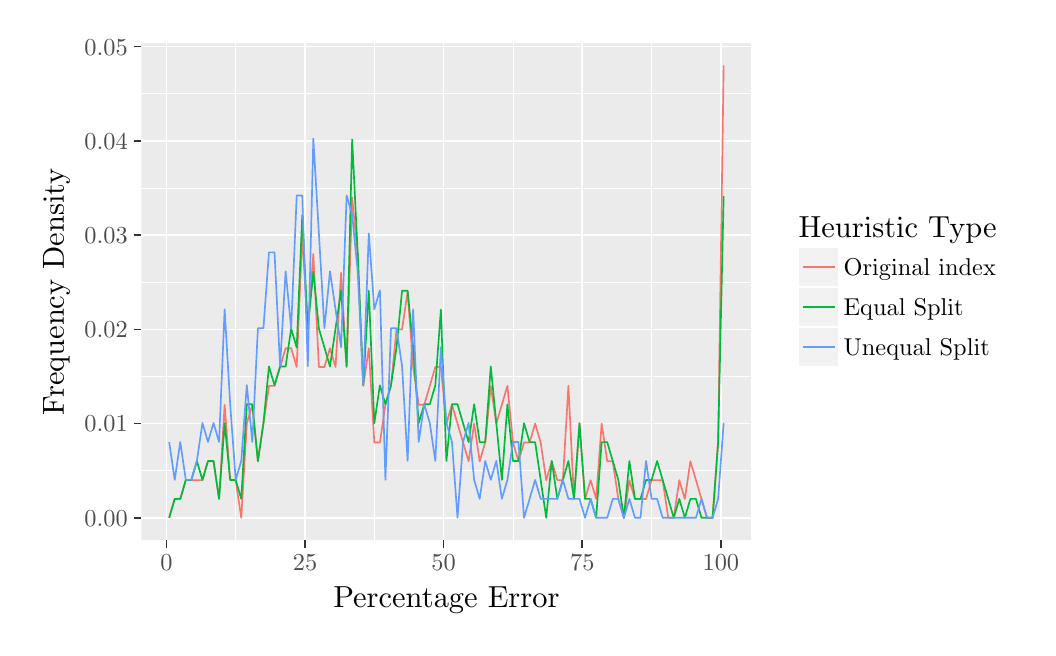
\begin{tikzpicture}[x=1pt,y=1pt]
\definecolor{fillColor}{RGB}{255,255,255}
\path[use as bounding box,fill=fillColor,fill opacity=0.00] (0,0) rectangle (361.35,216.81);
\begin{scope}
\path[clip] (  0.00,  0.00) rectangle (361.35,216.81);
\definecolor{drawColor}{RGB}{255,255,255}
\definecolor{fillColor}{RGB}{255,255,255}

\path[draw=drawColor,line width= 0.6pt,line join=round,line cap=round,fill=fillColor] (  0.00,  0.00) rectangle (361.35,216.81);
\end{scope}
\begin{scope}
\path[clip] ( 41.11, 31.53) rectangle (261.51,211.31);
\definecolor{fillColor}{gray}{0.92}

\path[fill=fillColor] ( 41.11, 31.53) rectangle (261.51,211.31);
\definecolor{drawColor}{RGB}{255,255,255}

\path[draw=drawColor,line width= 0.3pt,line join=round] ( 41.11, 56.73) --
	(261.51, 56.73);

\path[draw=drawColor,line width= 0.3pt,line join=round] ( 41.11, 90.78) --
	(261.51, 90.78);

\path[draw=drawColor,line width= 0.3pt,line join=round] ( 41.11,124.83) --
	(261.51,124.83);

\path[draw=drawColor,line width= 0.3pt,line join=round] ( 41.11,158.87) --
	(261.51,158.87);

\path[draw=drawColor,line width= 0.3pt,line join=round] ( 41.11,192.92) --
	(261.51,192.92);

\path[draw=drawColor,line width= 0.3pt,line join=round] ( 75.17, 31.53) --
	( 75.17,211.31);

\path[draw=drawColor,line width= 0.3pt,line join=round] (125.26, 31.53) --
	(125.26,211.31);

\path[draw=drawColor,line width= 0.3pt,line join=round] (175.36, 31.53) --
	(175.36,211.31);

\path[draw=drawColor,line width= 0.3pt,line join=round] (225.45, 31.53) --
	(225.45,211.31);

\path[draw=drawColor,line width= 0.6pt,line join=round] ( 41.11, 39.70) --
	(261.51, 39.70);

\path[draw=drawColor,line width= 0.6pt,line join=round] ( 41.11, 73.75) --
	(261.51, 73.75);

\path[draw=drawColor,line width= 0.6pt,line join=round] ( 41.11,107.80) --
	(261.51,107.80);

\path[draw=drawColor,line width= 0.6pt,line join=round] ( 41.11,141.85) --
	(261.51,141.85);

\path[draw=drawColor,line width= 0.6pt,line join=round] ( 41.11,175.90) --
	(261.51,175.90);

\path[draw=drawColor,line width= 0.6pt,line join=round] ( 41.11,209.95) --
	(261.51,209.95);

\path[draw=drawColor,line width= 0.6pt,line join=round] ( 50.13, 31.53) --
	( 50.13,211.31);

\path[draw=drawColor,line width= 0.6pt,line join=round] (100.22, 31.53) --
	(100.22,211.31);

\path[draw=drawColor,line width= 0.6pt,line join=round] (150.31, 31.53) --
	(150.31,211.31);

\path[draw=drawColor,line width= 0.6pt,line join=round] (200.40, 31.53) --
	(200.40,211.31);

\path[draw=drawColor,line width= 0.6pt,line join=round] (250.49, 31.53) --
	(250.49,211.31);
\definecolor{drawColor}{RGB}{248,118,109}

\path[draw=drawColor,line width= 0.6pt,line join=round] ( 51.13, 39.70) --
	( 53.13, 46.51) --
	( 55.14, 46.51) --
	( 57.14, 53.32) --
	( 59.14, 53.32) --
	( 61.15, 53.32) --
	( 63.15, 53.32) --
	( 65.15, 60.13) --
	( 67.16, 60.13) --
	( 69.16, 46.51) --
	( 71.17, 80.56) --
	( 73.17, 53.32) --
	( 75.17, 53.32) --
	( 77.18, 39.70) --
	( 79.18, 73.75) --
	( 81.18, 80.56) --
	( 83.19, 60.13) --
	( 85.19, 73.75) --
	( 87.19, 87.37) --
	( 89.20, 87.37) --
	( 91.20, 94.18) --
	( 93.21,100.99) --
	( 95.21,100.99) --
	( 97.21, 94.18) --
	( 99.22,141.85) --
	(101.22,107.80) --
	(103.22,135.04) --
	(105.23, 94.18) --
	(107.23, 94.18) --
	(109.24,100.99) --
	(111.24, 94.18) --
	(113.24,128.23) --
	(115.25, 94.18) --
	(117.25,155.47) --
	(119.25,135.04) --
	(121.26, 87.37) --
	(123.26,100.99) --
	(125.26, 66.94) --
	(127.27, 66.94) --
	(129.27, 80.56) --
	(131.28, 87.37) --
	(133.28,107.80) --
	(135.28,107.80) --
	(137.29,121.42) --
	(139.29, 94.18) --
	(141.29, 80.56) --
	(143.30, 80.56) --
	(145.30, 87.37) --
	(147.30, 94.18) --
	(149.31, 94.18) --
	(151.31, 73.75) --
	(153.32, 80.56) --
	(155.32, 73.75) --
	(157.32, 66.94) --
	(159.33, 60.13) --
	(161.33, 73.75) --
	(163.33, 60.13) --
	(165.34, 66.94) --
	(167.34, 87.37) --
	(169.34, 73.75) --
	(171.35, 80.56) --
	(173.35, 87.37) --
	(175.36, 66.94) --
	(177.36, 60.13) --
	(179.36, 66.94) --
	(181.37, 66.94) --
	(183.37, 73.75) --
	(185.37, 66.94) --
	(187.38, 53.32) --
	(189.38, 60.13) --
	(191.39, 53.32) --
	(193.39, 53.32) --
	(195.39, 87.37) --
	(197.40, 46.51) --
	(199.40, 73.75) --
	(201.40, 46.51) --
	(203.41, 53.32) --
	(205.41, 46.51) --
	(207.41, 73.75) --
	(209.42, 60.13) --
	(211.42, 60.13) --
	(213.43, 46.51) --
	(215.43, 39.70) --
	(217.43, 53.32) --
	(219.44, 46.51) --
	(221.44, 46.51) --
	(223.44, 46.51) --
	(225.45, 53.32) --
	(227.45, 53.32) --
	(229.45, 53.32) --
	(231.46, 39.70) --
	(233.46, 39.70) --
	(235.47, 53.32) --
	(237.47, 46.51) --
	(239.47, 60.13) --
	(241.48, 53.32) --
	(243.48, 46.51) --
	(245.48, 39.70) --
	(247.49, 39.70) --
	(249.49, 66.94) --
	(251.49,203.14);
\definecolor{drawColor}{RGB}{0,186,56}

\path[draw=drawColor,line width= 0.6pt,line join=round] ( 51.13, 39.70) --
	( 53.13, 46.54) --
	( 55.14, 46.54) --
	( 57.14, 53.38) --
	( 59.14, 53.38) --
	( 61.15, 60.21) --
	( 63.15, 53.38) --
	( 65.15, 60.21) --
	( 67.16, 60.21) --
	( 69.16, 46.54) --
	( 71.17, 73.89) --
	( 73.17, 53.38) --
	( 75.17, 53.38) --
	( 77.18, 46.54) --
	( 79.18, 80.73) --
	( 81.18, 80.73) --
	( 83.19, 60.21) --
	( 85.19, 73.89) --
	( 87.19, 94.40) --
	( 89.20, 87.56) --
	( 91.20, 94.40) --
	( 93.21, 94.40) --
	( 95.21,108.07) --
	( 97.21,101.24) --
	( 99.22,149.10) --
	(101.22,108.07) --
	(103.22,128.59) --
	(105.23,108.07) --
	(107.23,101.24) --
	(109.24, 94.40) --
	(111.24,108.07) --
	(113.24,121.75) --
	(115.25, 94.40) --
	(117.25,176.45) --
	(119.25,135.42) --
	(121.26, 87.56) --
	(123.26,121.75) --
	(125.26, 73.89) --
	(127.27, 87.56) --
	(129.27, 80.73) --
	(131.28, 87.56) --
	(133.28,101.24) --
	(135.28,121.75) --
	(137.29,121.75) --
	(139.29,101.24) --
	(141.29, 73.89) --
	(143.30, 80.73) --
	(145.30, 80.73) --
	(147.30, 87.56) --
	(149.31,114.91) --
	(151.31, 60.21) --
	(153.32, 80.73) --
	(155.32, 80.73) --
	(157.32, 73.89) --
	(159.33, 67.05) --
	(161.33, 80.73) --
	(163.33, 67.05) --
	(165.34, 67.05) --
	(167.34, 94.40) --
	(169.34, 73.89) --
	(171.35, 53.38) --
	(173.35, 80.73) --
	(175.36, 60.21) --
	(177.36, 60.21) --
	(179.36, 73.89) --
	(181.37, 67.05) --
	(183.37, 67.05) --
	(185.37, 53.38) --
	(187.38, 39.70) --
	(189.38, 60.21) --
	(191.39, 46.54) --
	(193.39, 53.38) --
	(195.39, 60.21) --
	(197.40, 46.54) --
	(199.40, 73.89) --
	(201.40, 46.54) --
	(203.41, 46.54) --
	(205.41, 39.70) --
	(207.41, 67.05) --
	(209.42, 67.05) --
	(211.42, 60.21) --
	(213.43, 53.38) --
	(215.43, 39.70) --
	(217.43, 60.21) --
	(219.44, 46.54) --
	(221.44, 46.54) --
	(223.44, 53.38) --
	(225.45, 53.38) --
	(227.45, 60.21) --
	(229.45, 53.38) --
	(231.46, 46.54) --
	(233.46, 39.70) --
	(235.47, 46.54) --
	(237.47, 39.70) --
	(239.47, 46.54) --
	(241.48, 46.54) --
	(243.48, 39.70) --
	(245.48, 39.70) --
	(247.49, 39.70) --
	(249.49, 67.05) --
	(251.49,155.93);
\definecolor{drawColor}{RGB}{97,156,255}

\path[draw=drawColor,line width= 0.6pt,line join=round] ( 51.13, 67.11) --
	( 53.13, 53.40) --
	( 55.14, 67.11) --
	( 57.14, 53.40) --
	( 59.14, 53.40) --
	( 61.15, 60.26) --
	( 63.15, 73.96) --
	( 65.15, 67.11) --
	( 67.16, 73.96) --
	( 69.16, 67.11) --
	( 71.17,115.06) --
	( 73.17, 80.81) --
	( 75.17, 53.40) --
	( 77.18, 60.26) --
	( 79.18, 87.66) --
	( 81.18, 67.11) --
	( 83.19,108.21) --
	( 85.19,108.21) --
	( 87.19,135.62) --
	( 89.20,135.62) --
	( 91.20, 94.51) --
	( 93.21,128.76) --
	( 95.21,108.21) --
	( 97.21,156.17) --
	( 99.22,156.17) --
	(101.22, 94.51) --
	(103.22,176.72) --
	(105.23,142.47) --
	(107.23,108.21) --
	(109.24,128.76) --
	(111.24,115.06) --
	(113.24,101.36) --
	(115.25,156.17) --
	(117.25,149.32) --
	(119.25,128.76) --
	(121.26, 87.66) --
	(123.26,142.47) --
	(125.26,115.06) --
	(127.27,121.91) --
	(129.27, 53.40) --
	(131.28,108.21) --
	(133.28,108.21) --
	(135.28, 94.51) --
	(137.29, 60.26) --
	(139.29,115.06) --
	(141.29, 67.11) --
	(143.30, 80.81) --
	(145.30, 73.96) --
	(147.30, 60.26) --
	(149.31,101.36) --
	(151.31, 73.96) --
	(153.32, 67.11) --
	(155.32, 39.70) --
	(157.32, 67.11) --
	(159.33, 73.96) --
	(161.33, 53.40) --
	(163.33, 46.55) --
	(165.34, 60.26) --
	(167.34, 53.40) --
	(169.34, 60.26) --
	(171.35, 46.55) --
	(173.35, 53.40) --
	(175.36, 67.11) --
	(177.36, 67.11) --
	(179.36, 39.70) --
	(181.37, 46.55) --
	(183.37, 53.40) --
	(185.37, 46.55) --
	(187.38, 46.55) --
	(189.38, 46.55) --
	(191.39, 46.55) --
	(193.39, 53.40) --
	(195.39, 46.55) --
	(197.40, 46.55) --
	(199.40, 46.55) --
	(201.40, 39.70) --
	(203.41, 46.55) --
	(205.41, 39.70) --
	(207.41, 39.70) --
	(209.42, 39.70) --
	(211.42, 46.55) --
	(213.43, 46.55) --
	(215.43, 39.70) --
	(217.43, 46.55) --
	(219.44, 39.70) --
	(221.44, 39.70) --
	(223.44, 60.26) --
	(225.45, 46.55) --
	(227.45, 46.55) --
	(229.45, 39.70) --
	(231.46, 39.70) --
	(233.46, 39.70) --
	(235.47, 39.70) --
	(237.47, 39.70) --
	(239.47, 39.70) --
	(241.48, 39.70) --
	(243.48, 46.55) --
	(245.48, 39.70) --
	(247.49, 39.70) --
	(249.49, 46.55) --
	(251.49, 73.96);
\end{scope}
\begin{scope}
\path[clip] (  0.00,  0.00) rectangle (361.35,216.81);
\definecolor{drawColor}{gray}{0.30}

\node[text=drawColor,anchor=base east,inner sep=0pt, outer sep=0pt, scale=  0.88] at ( 36.16, 36.67) {0.00};

\node[text=drawColor,anchor=base east,inner sep=0pt, outer sep=0pt, scale=  0.88] at ( 36.16, 70.72) {0.01};

\node[text=drawColor,anchor=base east,inner sep=0pt, outer sep=0pt, scale=  0.88] at ( 36.16,104.77) {0.02};

\node[text=drawColor,anchor=base east,inner sep=0pt, outer sep=0pt, scale=  0.88] at ( 36.16,138.82) {0.03};

\node[text=drawColor,anchor=base east,inner sep=0pt, outer sep=0pt, scale=  0.88] at ( 36.16,172.87) {0.04};

\node[text=drawColor,anchor=base east,inner sep=0pt, outer sep=0pt, scale=  0.88] at ( 36.16,206.92) {0.05};
\end{scope}
\begin{scope}
\path[clip] (  0.00,  0.00) rectangle (361.35,216.81);
\definecolor{drawColor}{gray}{0.20}

\path[draw=drawColor,line width= 0.6pt,line join=round] ( 38.36, 39.70) --
	( 41.11, 39.70);

\path[draw=drawColor,line width= 0.6pt,line join=round] ( 38.36, 73.75) --
	( 41.11, 73.75);

\path[draw=drawColor,line width= 0.6pt,line join=round] ( 38.36,107.80) --
	( 41.11,107.80);

\path[draw=drawColor,line width= 0.6pt,line join=round] ( 38.36,141.85) --
	( 41.11,141.85);

\path[draw=drawColor,line width= 0.6pt,line join=round] ( 38.36,175.90) --
	( 41.11,175.90);

\path[draw=drawColor,line width= 0.6pt,line join=round] ( 38.36,209.95) --
	( 41.11,209.95);
\end{scope}
\begin{scope}
\path[clip] (  0.00,  0.00) rectangle (361.35,216.81);
\definecolor{drawColor}{gray}{0.20}

\path[draw=drawColor,line width= 0.6pt,line join=round] ( 50.13, 28.78) --
	( 50.13, 31.53);

\path[draw=drawColor,line width= 0.6pt,line join=round] (100.22, 28.78) --
	(100.22, 31.53);

\path[draw=drawColor,line width= 0.6pt,line join=round] (150.31, 28.78) --
	(150.31, 31.53);

\path[draw=drawColor,line width= 0.6pt,line join=round] (200.40, 28.78) --
	(200.40, 31.53);

\path[draw=drawColor,line width= 0.6pt,line join=round] (250.49, 28.78) --
	(250.49, 31.53);
\end{scope}
\begin{scope}
\path[clip] (  0.00,  0.00) rectangle (361.35,216.81);
\definecolor{drawColor}{gray}{0.30}

\node[text=drawColor,anchor=base,inner sep=0pt, outer sep=0pt, scale=  0.88] at ( 50.13, 20.52) {0};

\node[text=drawColor,anchor=base,inner sep=0pt, outer sep=0pt, scale=  0.88] at (100.22, 20.52) {25};

\node[text=drawColor,anchor=base,inner sep=0pt, outer sep=0pt, scale=  0.88] at (150.31, 20.52) {50};

\node[text=drawColor,anchor=base,inner sep=0pt, outer sep=0pt, scale=  0.88] at (200.40, 20.52) {75};

\node[text=drawColor,anchor=base,inner sep=0pt, outer sep=0pt, scale=  0.88] at (250.49, 20.52) {100};
\end{scope}
\begin{scope}
\path[clip] (  0.00,  0.00) rectangle (361.35,216.81);
\definecolor{drawColor}{RGB}{0,0,0}

\node[text=drawColor,anchor=base,inner sep=0pt, outer sep=0pt, scale=  1.10] at (151.31,  7.44) {Percentage Error};
\end{scope}
\begin{scope}
\path[clip] (  0.00,  0.00) rectangle (361.35,216.81);
\definecolor{drawColor}{RGB}{0,0,0}

\node[text=drawColor,rotate= 90.00,anchor=base,inner sep=0pt, outer sep=0pt, scale=  1.10] at ( 13.08,121.42) {Frequency Density};
\end{scope}
\begin{scope}
\path[clip] (  0.00,  0.00) rectangle (361.35,216.81);
\definecolor{fillColor}{RGB}{255,255,255}

\path[fill=fillColor] (272.89, 88.45) rectangle (355.85,154.39);
\end{scope}
\begin{scope}
\path[clip] (  0.00,  0.00) rectangle (361.35,216.81);
\definecolor{drawColor}{RGB}{0,0,0}

\node[text=drawColor,anchor=base west,inner sep=0pt, outer sep=0pt, scale=  1.10] at (278.58,141.12) {Heuristic Type};
\end{scope}
\begin{scope}
\path[clip] (  0.00,  0.00) rectangle (361.35,216.81);
\definecolor{drawColor}{RGB}{255,255,255}
\definecolor{fillColor}{gray}{0.95}

\path[draw=drawColor,line width= 0.6pt,line join=round,line cap=round,fill=fillColor] (278.58,123.05) rectangle (293.04,137.51);
\end{scope}
\begin{scope}
\path[clip] (  0.00,  0.00) rectangle (361.35,216.81);
\definecolor{drawColor}{RGB}{248,118,109}

\path[draw=drawColor,line width= 0.6pt,line join=round] (280.03,130.28) -- (291.59,130.28);
\end{scope}
\begin{scope}
\path[clip] (  0.00,  0.00) rectangle (361.35,216.81);
\definecolor{drawColor}{RGB}{255,255,255}
\definecolor{fillColor}{gray}{0.95}

\path[draw=drawColor,line width= 0.6pt,line join=round,line cap=round,fill=fillColor] (278.58,108.60) rectangle (293.04,123.05);
\end{scope}
\begin{scope}
\path[clip] (  0.00,  0.00) rectangle (361.35,216.81);
\definecolor{drawColor}{RGB}{0,186,56}

\path[draw=drawColor,line width= 0.6pt,line join=round] (280.03,115.83) -- (291.59,115.83);
\end{scope}
\begin{scope}
\path[clip] (  0.00,  0.00) rectangle (361.35,216.81);
\definecolor{drawColor}{RGB}{255,255,255}
\definecolor{fillColor}{gray}{0.95}

\path[draw=drawColor,line width= 0.6pt,line join=round,line cap=round,fill=fillColor] (278.58, 94.14) rectangle (293.04,108.60);
\end{scope}
\begin{scope}
\path[clip] (  0.00,  0.00) rectangle (361.35,216.81);
\definecolor{drawColor}{RGB}{97,156,255}

\path[draw=drawColor,line width= 0.6pt,line join=round] (280.03,101.37) -- (291.59,101.37);
\end{scope}
\begin{scope}
\path[clip] (  0.00,  0.00) rectangle (361.35,216.81);
\definecolor{drawColor}{RGB}{0,0,0}

\node[text=drawColor,anchor=base west,inner sep=0pt, outer sep=0pt, scale=  0.88] at (294.85,127.25) {Original index};
\end{scope}
\begin{scope}
\path[clip] (  0.00,  0.00) rectangle (361.35,216.81);
\definecolor{drawColor}{RGB}{0,0,0}

\node[text=drawColor,anchor=base west,inner sep=0pt, outer sep=0pt, scale=  0.88] at (294.85,112.80) {Equal Split};
\end{scope}
\begin{scope}
\path[clip] (  0.00,  0.00) rectangle (361.35,216.81);
\definecolor{drawColor}{RGB}{0,0,0}

\node[text=drawColor,anchor=base west,inner sep=0pt, outer sep=0pt, scale=  0.88] at (294.85, 98.34) {Unequal Split};
\end{scope}
\end{tikzpicture}

%\caption{Equal and unequal splitting against original for benefit heuristic}
%\label{Figure:Benefit splitting experiment}
%\end{myfigure}
%
%Our numerical experiments would seem to indicate that splitting the index amongst all states, $s \leq B$ does not seem to provide any increase in the heuristics performance.

\section{Strategic Patroller with Random Attackers and Local-observations}
\label{Section:Patrolling games with random attackers and local-observations}
We now look at altering the work summarized in Section \ref{Section:Review of patrolling problem with random attackers} to incorporate suspicious behaviour of attackers who arrive while the patroller is present.

\subsection{Altering the problem for an instantaneously moving patroller}
We may now wish to alter the standard set-up of a patroller moving at unit speed along the edges, if the guard was flicking through live-video feeds, while unit time is spend on each feed, there is no transition time between nodes. To more closely represent this we will alter the theory to account for an instantaneously moving patroller. Figure \ref{Figure:Example of timing for instantaneously moving patroller} shows an example of the timing of a patroller who does not have to wait the one time unit to move along edges.

\begin{myfigure}
\begin{center}
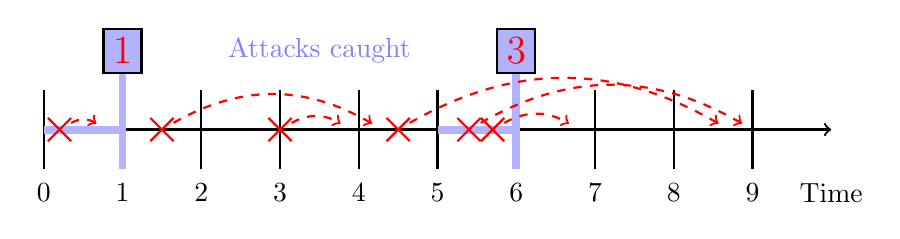
\begin{tikzpicture}[-,auto,node distance=2cm,
                    thick,main node/.style={rectangle,draw,font=\sffamily\Large\bfseries}]

%DRAWING Base line

 \draw[->] (0,0)--(10,0);
 
 \foreach \x in {0,...,9}
 {\draw  (\x,0.5)--(\x,-0.5) ;
  \node (TimeLabel\x) at (\x,-0.8) {$\x$};} 
  
  \node (TimeLabel) at (10,-0.8) {Time};

%Inserting patroller and attackers
  
    \node[main node,fill=blue!30] (Pat1) at (1,1) {\textcolor{red}{$1$}};
  \draw[color=blue!30,line width=0.1cm] (Pat1)--(1,-0.5);
  \draw[color=blue!30,line width=0.1cm] (0,0)--(1,0);
  
  \node[main node,fill=blue!30] (Pat2) at (6,1) {\textcolor{red}{$3$}};
  \draw[color=blue!30,line width=0.1cm] (Pat2)--(6,-0.5);
  \draw[color=blue!30,line width=0.1cm] (5,0)--(6,0);
  
  
  \node[cross=5pt,color=red] (AttackStart1) at (0.2,0) {};
  \node (AttackEnd1) at (0.8,0) {};
  \draw[bend left,color=red,->,dashed] (AttackStart1) to (AttackEnd1);
  
  \node[cross=5pt,color=red] (AttackStart2) at (1.5,0) {};
  \node (AttackEnd2) at (4.3,0) {};
  \draw[bend left,color=red,->,dashed] (AttackStart2) to (AttackEnd2);
  
  \node[cross=5pt,color=red] (AttackStart3) at (3,0) {};
  \node (AttackEnd3) at (3.9,0) {};
  \draw[bend left,color=red,->,dashed] (AttackStart3) to (AttackEnd3);
  
  \node[cross=5pt,color=red] (AttackStart4) at (4.5,0) {};
  \node (AttackEnd4) at (8.7,0) {};
  \draw[bend left,color=red,->,dashed] (AttackStart4) to (AttackEnd4);
  
  \node[cross=5pt,color=red] (AttackStart5) at (5.4,0) {};
  \node (AttackEnd5) at (9,0) {};
  \draw[bend left,color=red,->,dashed] (AttackStart5) to (AttackEnd5);
  
  \node[cross=5pt,color=red] (AttackStart6) at (5.7,0) {};
  \node (AttackEnd6) at (6.8,0) {};
  \draw[bend left,color=red,->,dashed] (AttackStart6) to (AttackEnd6);
  
  
  \node (AttacksCaught) at (3.5,1) {\textcolor{blue!50}{Attacks caught}};
  
       
\end{tikzpicture}
\end{center}
\caption{Example of timing at a node for an instantaneously moving patroller.}
\label{Figure:Example of timing for instantaneously moving patroller}
\end{myfigure} 

While the standard set-up remains mostly intact, the cost function is slightly altered to accommodate this change. We note there is now a difference in cost depending on if the node is visited or not.

\begin{align*}
C_{j}(\bm{s},i) &= \begin{cases}
0  \text{ if } j=i \\
c_{j} \lambda_{j} \int_{s_{j}-1}^{s_{j}} P(X_{j} \leq t) dt \text{ if } j \neq i \\
\end{cases}
\end{align*}

This change does not affect the theory too much, the problem can still be reduced to the single node version of the instantaneous moving problem, by implementing the TR-constraint and using lagrangian relaxation. We now state the changes in the single node formulation,

\begin{align*}
&f(k) \equiv \frac{c \lambda \int_{0}^{k-1} P(X \leq t) dt + \omega}{k} \\
&W(k) \equiv c \lambda \left( k \int_{k-1}^{k} P(X \leq t) dt - \int_{0}^{k-1} P(X \leq t) dt \right)
\end{align*}

\begin{note}
$W(0)=0$ still but for $k \geq B+1$ $W(k)= c \lambda (1+E[X])$
\end{note}

Using this new definition of $W(k)$, Theorem \ref{Theorem:Single node optimal policy} still holds and gives us the optimal policy. Hence suggesting an index of

\begin{align*}
W_{i}(\bm{s}) \equiv c_{i} \lambda_{i} \left( s_{i} \int_{s_{i}-1}^{s_{i}} P(X_{i} \leq t) dt - \int_{0}^{s_{i}-1} P(X_{i} \leq t) dt \right)
\end{align*}

We should perform a numerical study to check that this index still performs well, however our code does not currently work for general distributions functions so this will be left to future work(section \ref{Section:Complete Numerical experiments for an instantaneously moving patroller})



\subsection{Altering problem to accommodate local-observable information}
Now that we have established a instantaneously moving patroller, we can now introduce the idea of local-observations, that is the patroller witnessing attackers arriving at their current node. We will assume that the attackers do not begin their attack immediately if they are aware of the patroller's presence when they arrive. For now we assume that any such attacker is only able to delay their attack to start at the beginning of the next time period, instead of waiting till the patroller leaves the node. Figure \ref{Figure:Example of local-observation graph diagram} shows shows an example of the current state on the graph, and figure \ref{Figure:Example of timing for instantaneous and local observations} shows shows an example of the timing at a node when the patroller arrives, with attackers delaying.

\begin{myfigure}
\begin{center}
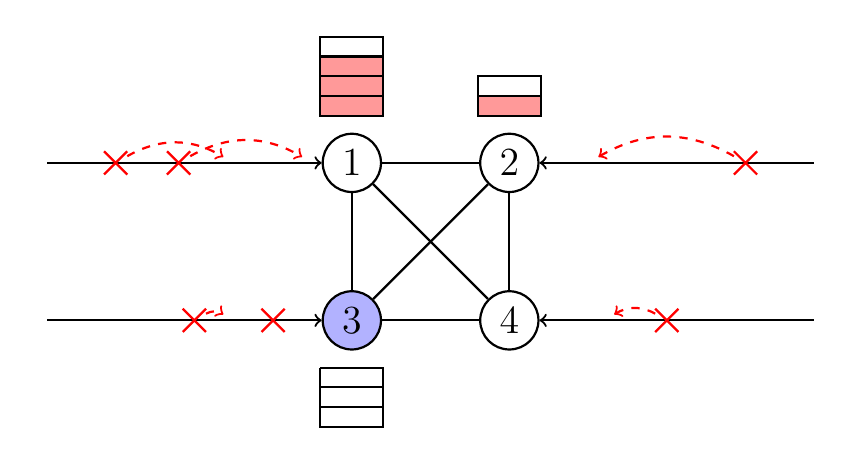
\begin{tikzpicture}[-,auto,node distance=2cm,
                    thick,main node/.style={circle,fill=white,draw,font=\sffamily\Large\bfseries}]

%DRAWING GRAPH
  \node[main node] (1) {$1$};
  \node[main node] (2) [right of=1] {$2$};
  \node[main node,fill=blue!30] (3) [below of=1]  {$3$};
  \node[main node] (4) [below of=2]  {$4$};

  \path[every node/.style={font=\sffamily}]
    (1) edge (2)
        edge (3)
        edge (4)
    (2) edge (3)
        edge (4)
    (3) edge (4);
  
  
%DRAWING ARRIVALS  
  \node (1ArrowStart) [shift={(-4,0)}] at (1) {};
  \draw[->] (1ArrowStart)--(1);
  
  \node[cross=5pt,color=red] (1Cross1) [shift={(-3,0)}] at (1) { };
  \node (1CrossEnd1) [shift={(-1.5,0)}] at (1) {};
  \draw[->,bend left,dashed,color=red] (1Cross1) to (1CrossEnd1);
  \node[cross=5pt,color=red] (1Cross2) [shift={(-2.2,0)}] at (1) { };
  \node (1CrossEnd2) [shift={(-0.5,0)}] at (1) {};
  \draw[->,bend left,dashed,color=red] (1Cross2) to (1CrossEnd2);
  
  \node (2ArrowStart) [shift={(4,0)}] at (2) {};
  \draw[->] (2ArrowStart)--(2);
  
  \node[cross=5pt,color=red] (2Cross1) [shift={(3,0)}] at (2) { };
  \node (2CrossEnd1) [shift={(1,0)}] at (2) {};
  \draw[->,bend right,dashed,color=red] (2Cross1) to (2CrossEnd1);

  \node (3ArrowStart) [shift={(-4,0)}] at (3) {};
  \draw[->] (3ArrowStart)--(3);
  
  \node[cross=5pt,color=red] (3Cross1) [shift={(-2,0)}] at (3) { };
  \node (3CrossEnd1) [shift={(-1.5,0)}] at (3) {};
  \draw[->,bend left,dashed,color=red] (3Cross1) to (3CrossEnd1);
  \node[cross=5pt,color=red] (3Cross1) [shift={(-1,0)}] at (3) { };
  
  \node (4ArrowStart) [shift={(4,0)}] at (4) {};
  \draw[->] (4ArrowStart)--(4);
  
  \node[cross=5pt,color=red] (4Cross1) [shift={(2,0)}] at (4) { };
  \node (4CrossEnd1) [shift={(1.2,0)}] at (4) {};
  \draw[->,bend right,dashed,color=red] (4Cross1) to (4CrossEnd1);
  
%Drawing Observable capacity boxes
 \node (1LowerLeft) [shift={(-0.4,0.6)}] at (1) { };
 \node (1LowerRight) [shift={(0.4,0.6)}] at (1) { };
 \node (1UpperLeft) [shift={(-0.4,1.6)}] at (1) { };
 \node (1UpperRight) [shift={(0.4,1.6)}] at (1) { }; 
 
 \draw[-] (1LowerLeft.center)--(1LowerRight.center)--(1UpperRight.center)
 --(1UpperLeft.center)--(1LowerLeft.center);
 
 \node (1FillPointLeft1) [shift={(0,0.25)}] at (1LowerLeft) { };
 \node (1FillPointRight1) [shift={(0,0.25)}] at (1LowerRight) { };
 \node (1FillPointLeft2) [shift={(0,0.5)}] at (1LowerLeft) { };
 \node (1FillPointRight2) [shift={(0,0.5)}] at (1LowerRight) { };
 \node (1FillPointLeft3) [shift={(0,0.75)}] at (1LowerLeft) { };
 \node (1FillPointRight3) [shift={(0,0.75)}] at (1LowerRight) { };

 \filldraw[fill=red!40!white, draw=black] (1LowerLeft) rectangle (1FillPointRight3);
 
 \draw[-] (1FillPointLeft1.center)--(1FillPointRight1.center);
 \draw[-] (1FillPointLeft2.center)--(1FillPointRight2.center);
 \draw[-] (1FillPointLeft3.center)--(1FillPointRight3.center);
 
 
 
 \node (2LowerLeft) [shift={(-0.4,0.6)}] at (2) { };
 \node (2LowerRight) [shift={(0.4,0.6)}] at (2) { };
 \node (2UpperLeft) [shift={(-0.4,1.1)}] at (2) { };
 \node (2UpperRight) [shift={(0.4,1.1)}] at (2) { }; 
 
 \draw[-] (2LowerLeft.center)--(2LowerRight.center)--(2UpperRight.center)
 --(2UpperLeft.center)--(2LowerLeft.center);
 
 \node (2FillPointLeft1) [shift={(0,0.25)}] at (2LowerLeft) { };
 \node (2FillPointRight1) [shift={(0,0.25)}] at (2LowerRight) { };

 \filldraw[fill=red!40!white, draw=black] (2LowerLeft) rectangle (2FillPointRight1);
 
 \draw[-] (1FillPointLeft1.center)--(1FillPointRight1.center);
 
 
 \node (3LowerLeft) [shift={(-0.4,-0.6)}] at (3) { };
 \node (3LowerRight) [shift={(0.4,-0.6)}] at (3) { };
 \node (3UpperLeft) [shift={(-0.4,-1.35)}] at (3) { };
 \node (3UpperRight) [shift={(0.4,-1.35)}] at (3) { }; 
 
 \draw[-] (3LowerLeft.center)--(3LowerRight.center)--(3UpperRight.center)
 --(3UpperLeft.center)--(3LowerLeft.center);
 
 \node (3FillPointLeft1) [shift={(0,-0.25)}] at (3LowerLeft) { };
 \node (3FillPointRight1) [shift={(0,-0.25)}] at (3LowerRight) { };
 \node (3FillPointLeft2) [shift={(0,-0.5)}] at (3LowerLeft) { };
 \node (3FillPointRight2) [shift={(0,-0.5)}] at (3LowerRight) { };

 
 \draw[-] (3FillPointLeft1.center)--(3FillPointRight1.center);
 \draw[-] (3FillPointLeft2.center)--(3FillPointRight2.center);
    
\end{tikzpicture}
\end{center}
\caption{Example of $G=(K_{4},\bm{X},\bm{b},\bm{\lambda},\bm{c})$ with patroller currently at node $3$.}
\label{Figure:Example of local-observation graph diagram}
\end{myfigure}


\begin{myfigure}
\begin{center}
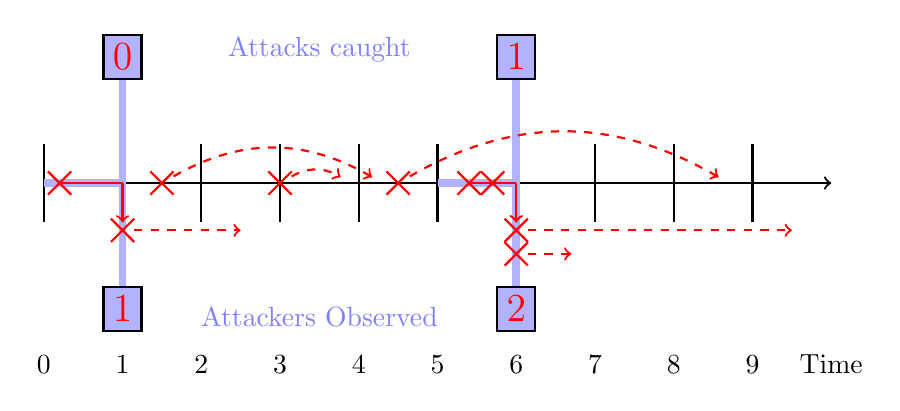
\begin{tikzpicture}[-,auto,node distance=2cm,
                    thick,main node/.style={rectangle,draw,font=\sffamily\Large\bfseries}]

%DRAWING Base line

 \draw[->] (0,0)--(10,0);
 
 \foreach \x in {0,...,9}
 {\draw  (\x,0.5)--(\x,-0.5) ;
  \node (TimeLabel\x) at (\x,-2.3) {$\x$};} 
  
  \node (TimeLabel) at (10,-2.3) {Time};

%Inserting patroller and attackers
  \node[main node,fill=blue!30] (Pat1) at (1,1.6) {\textcolor{red}{$0$}};
  \node[main node,fill=blue!30] (PatObs1) at (1,-1.6) {\textcolor{red}{$1$}};
  \draw[color=blue!30,line width=0.1cm] (Pat1)--(PatObs1);
  \draw[color=blue!30,line width=0.1cm] (0,0)--(1,0);
  
  \node[main node,fill=blue!30] (Pat2) at (6,1.6) {\textcolor{red}{$1$}};
  \node[main node,fill=blue!30] (PatObs2) at (6,-1.6) {\textcolor{red}{$2$}};
  \draw[color=blue!30,line width=0.1cm] (Pat2)--(PatObs2);
  \draw[color=blue!30,line width=0.1cm] (5,0)--(6,0);
  
  
  \node[cross=5pt,color=red] (AttackStart1) at (0.2,0) {};
  \draw[-,color=red] (AttackStart1.center) to (1,0);
  \draw[->,color=red] (1,0) to (1,-0.5);
  \node[cross=5pt,color=red] (NewAttackStart1) at (1,-0.6) {};
  \draw[->,color=red,dashed] (NewAttackStart1) to (2.5,-0.6);
  
  \node[cross=5pt,color=red] (AttackStart2) at (1.5,0) {};
  \node (AttackEnd2) at (4.3,0) {};
  \draw[bend left,color=red,->,dashed] (AttackStart2) to (AttackEnd2);
  
  \node[cross=5pt,color=red] (AttackStart3) at (3,0) {};
  \node (AttackEnd3) at (3.9,0) {};
  \draw[bend left,color=red,->,dashed] (AttackStart3) to (AttackEnd3);
  
  \node[cross=5pt,color=red] (AttackStart4) at (4.5,0) {};
  \node (AttackEnd4) at (8.7,0) {};
  \draw[bend left,color=red,->,dashed] (AttackStart4) to (AttackEnd4);
  
  \node[cross=5pt,color=red] (AttackStart5) at (5.4,0) {};
  \draw[-,color=red] (AttackStart5.center) to (6,0);
  \draw[->,color=red] (6,0) to (6,-0.5);
  \node[cross=5pt,color=red] (NewAttackStart5) at (6,-0.6) {};
  \draw[->,color=red,dashed] (NewAttackStart5) to (9.5,-0.6);
  
  
  \node[cross=5pt,color=red] (AttackStart6) at (5.7,0) {};
  \draw[-,color=red] (AttackStart6.center) to (6,0);
  \draw[->,color=red] (6,0) to (6,-0.5);
  \node[cross=5pt,color=red] (NewAttackStart5) at (6,-0.9) {};
  \draw[->,color=red,dashed] (NewAttackStart5) to (6.7,-0.9);

 \node (AttacksCaught) at (3.5,1.7) {\textcolor{blue!50}{Attacks caught}};
 
 \node (AttacksObs) at (3.5,-1.7) {\textcolor{blue!50}{Attackers Observed}};
  
       
\end{tikzpicture}
\end{center}
\caption{Example of timing at a node for an instantaneously moving patroller with local-observations.}
\label{Figure:Example of timing for instantaneous and local observations}
\end{myfigure}

The problem can still be formulated as a MDP, however the states now need to hold the information about how many attackers where observed when the node was last visited, in addition to when it was last visited. Our state space is

$$\Omega= \{ (\bm{s},\bm{v})=(s_{1},...,s_{n},v_{1},...,v_{n}) \, | \, s_{i}=1,2,...., \; v_{i}=0,1,...  \text{ for } i=1,...,n\}$$

Where as before, $s_{i}$ denotes the time since the last decision to visit node $i$ was taken and the newly introduced $v_{i}$ denotes how many attackers where observed when the patroller last visited node $i$.The current node is $l(\bm{s},\bm{v})=\argmin_{i} s_{i}$ and the decisions from $(\bm{s},\bm{v})$ are still adjacent node, $\mathcal{A}(\bm{s},\bm{v})$. The transition when node $i$ is chosen to move to are $\phi(\bm{s},\bm{v},i)=(\widetilde{\bm{s}},\widetilde{\bm{v}})$, where; $\widetilde{s}_{i}=1$,  $\widetilde{s}_{j}=s_{j}+1 \; \forall j \neq i$, $\widetilde{v}_{i} \sim Po(\lambda_{i})$ and $\widetilde{v}_{j}=v_{j} \; \forall j \neq i$.

That is the $\bm{s}$ state transitions as before, and the $\bm{v}$ state updates the chosen node to be the amount observed while the patroller is at the node, which is drawn from a Poisson distribution of rate $\lambda_{i}$ due to the arrivals being a Poisson Process.

Again the future of the process is independent of its past, so we can formulate its movement as an MC and hence the patrollers problem is a MDP.

The patroller incurs cost $c_{j}$ for all successful attacks at node $j$. A successful attack will fall into two categories; an observed attack or an attacker who arrived. We simply sum the expected costs of both types of attacker to work out the cost at a node for the next unit time, given we choose to move to node $i$.

\begin{align*}
C_{j}(\bm{s},\bm{v},i) &= \begin{cases}
0  \text{ if } j=i \\
\underbrace{c_{j} v_{j} P(s_{j}-1 < X_{j} \leq s_{j})}_{\text{Observed finishing}} + \underbrace{c_{j} \lambda_{j} \int_{s_{j}-1}^{s_{j}} P(X_{j} \leq t) dt}_{\text{Arrivals finishing}} \text{ if } j \neq i \\
\end{cases}
\end{align*}

We run into the same problem as before, with a countably infinite state space, $\Omega$, we therefore wish to bound ourselves to a finite state space. As before we can bound the attack times, defining $B_{j}$ as in \ref{Equation:Definition of attack time bound}, but this only partially solves our problem, as it bounds the $\bm{s}$ part of the state space but not the $\bm{v}$ part.

To bound $\bm{v}$ we introduce a observable capacity, $\bm{b}$, where $b_{i}$ is the maximum number of local-observations at node $i$. We assume that all other attackers fail once this capacity is reached.

\begin{figure}[H]
\begin{center}
\resizebox{0.8\linewidth}{!}{
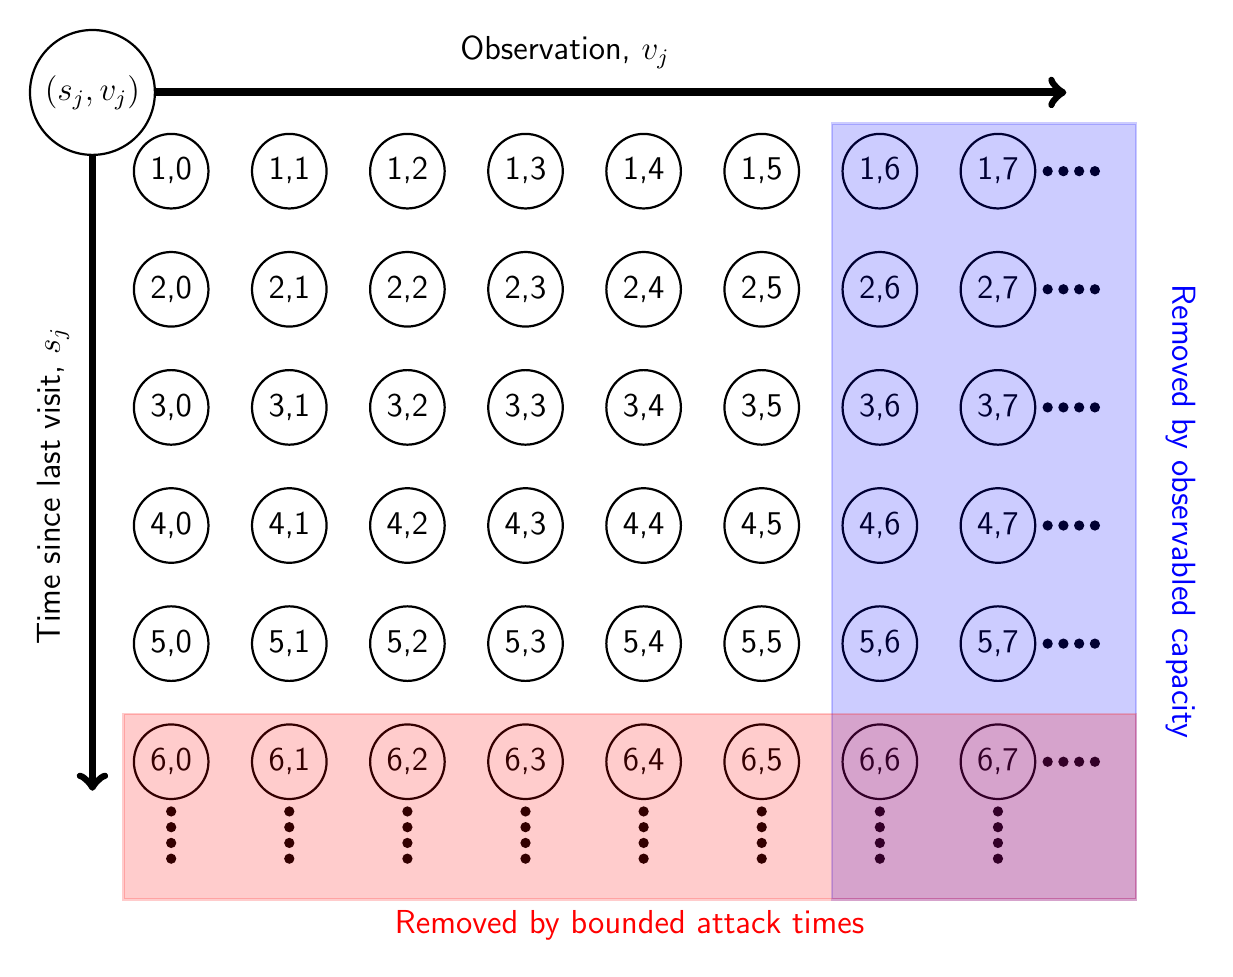
\begin{tikzpicture}[-,auto,node distance=1cm,
                    thick,main node/.style={circle,fill=white,draw,font=\sffamily\large,minimum size=0.5cm}]
 \foreach \x in {0,...,7}
    \foreach \y in {0,...,5} 
       {\pgfmathtruncatemacro{\label}{\x - 5 *  \y +21}
        \pgfmathtruncatemacro{\v}{\x}
        \pgfmathtruncatemacro{\s}{6-\y}
       \node [main node]  (\x\y) at (1.5*\x,1.5*\y) {\s,\v};} 

\node (XaxisLeft) [shift={(-0.5,1)}] at (05) {};
\node (XaxisRight) [shift={(1,1)}] at (75) {};

\node (YaxisBottom) [shift={(-1,-0.5)}] at (00) {};
\node (YaxisTop) [shift={(-1,1)}] at (05) {};

\draw[->,line width=1mm] (XaxisLeft)--(XaxisRight);
\draw[->,line width=1mm] (YaxisTop)--(YaxisBottom);

\node[font=\sffamily\large] (OLabel) [shift={(0.5,1.5)}] at (35) {Observation, $v_{j}$};
\node[font=\sffamily\large] (SLabel) [shift={(-1.5,0.5)}] at (02) {\rotatebox{90}{Time since last visit, $s_{j}$}};

\node[main node] (Example) [shift={(-1,1)}] at (05) {$(s_{j},v_{j})$};

\foreach \y in {0,...,5}
{\node (DottedStart\y) [shift={(0.5,0)}] at (7\y) {};
 \node (DottedEnd\y) [shift={(1.5,0)}] at (7\y) {};
 \draw[decorate sep={1mm}{2mm},fill] (DottedStart\y)--(DottedEnd\y);}
 
\foreach \x in {0,...,7}
{\node (\x DottedStart) [shift={(0,-0.5)}] at (\x0) {};
 \node (\x DottedEnd) [shift={(0,-1.5)}] at (\x0) {};
 \draw[decorate sep={1mm}{2mm},fill] (\x DottedStart)--(\x DottedEnd);
}

\node (Box1) [draw,thick,fit=(65) (60) (DottedEnd5) (DottedEnd0) (6DottedEnd) (7DottedEnd),fill,blue,opacity=0.2] {};

\node (Box2) [draw,thick,fit=(00) (70)(DottedEnd0) (0DottedEnd) (7DottedEnd),fill,red,opacity=0.2] {};

\node[font=\sffamily\large,color=blue] (Box1Text) [shift={(2.5,0)}] at (Box1) {\rotatebox{270}{Removed by observabled capacity}};

\node[font=\sffamily\large,color=red] (Box2Text) [shift={(0,-1.5)}] at (Box2) {Removed by bounded attack times};           

\end{tikzpicture}
}
\end{center}
\caption{State space diagram for node $j$, with \textcolor{blue}{$b_{j}=5$} and \textcolor{red}{$B_{j}=4$} (e.g. $X_{j} \leq 3.7$).}
\end{figure}

This change to a finite state space, $\Omega = \{ (\bm{s},\bm{v})=(s_{1},...,s_{n},v_{1},...,v_{n}) \, | \, s_{i}=1,2,....,B_{i}+1 \; v_{i}=0,1,...,b_{i}  \text{ for } i=1,...,n\}$ and caps the transitions. That is that $\widetilde{s}_{j}= \min \{s_{j}+1, B_{j}+1 \}$ and $\widetilde{v}_{i} \sim TPo(\lambda_{i},b_{i)}$, where $TPo(\lambda,b)$ is the truncated Poisson distribution, with all the tail probability at the value $b_{i}$. I.e.

\begin{align*}
P(TPo(\lambda,b)=\begin{cases}
P(Po(\lambda) \text{ if } i \neq b \\
P(Po(\lambda) \geq i) \text{ if } i=b \\
0 \text{ Otherwise}
\end{cases}
\end{align*}

Even though the state space is now finite, the transitions are not deterministic, so a cyclic behaviour is not induced when the same state is reached again. For notational purposes we will still use $\phi^{k}_{\pi}(\bm{s}_{0},\bm{v}_{0})$ to be the state after $k$ transitions from $(\bm{s}_{0},\bm{v}_{0})$. We might be able to get some cycles that happen with some probability instead, however we leave this idea of cycles behind for now (and state that it is future work considered in section \ref{Section:Complete Numerical experiments for an instantaneously moving patroller} because it is useful to better evaluate policies).

This problem, as before, can be solved by standard techniques such as value iteration or linear programming to compute the long-run average cost. This is left to Appendix \ref{Appendix:Optimal Solution for Random Attacker with Local-Observations}.

We can then use the standard reduction tools of making the problem into a MN problem and then applying the TR constraint and/or the Lagrangian relaxation. We shall therefore focus on the Lagrangian relaxation which is equivalent to the single node problem.

We wish to minimize, $V(\pi)+\omega \mu(\pi)$. Our state space is more complicated than before due to the inclusion of the time since it was last visited and the amount of local-observations made when it was last visited.

\subsection{Deterministic attack time assumption}
\label{Section:Deterministic attack time assumption}
Because our state space is hard to deal with, in the single node problem, we shall reduce the problem, by assuming that the attack times are deterministic, that is $P(X=x)=1$, this reduces our cost function to

\begin{align*}
C_{j}(\bm{s},\bm{v},i)=\begin{cases}
c_{j} \lambda_{j} R_{j} + c_{j} v_{j}  \text{ for } s_{j}=B_{j},i \neq j \\ 
c_{j} \lambda_{j} \text{ for } s_{j}=B_{j}+1,i \neq j  \\
0 \text{ Otherwise} \\
\end{cases}
\end{align*}
Where $R_{j}=B_{j}-x_{j}$. We see that we only worry about incurring costs in states when $s_{i}=B_{i}$ or $B_{i}+1$ for some $i$.

This allows us to see a clear solution to the single node problem.

\subsection{Single node solution}
\label{Section:Single node solution}
Again we wish to minimize the long-run average cost, paying $\omega$ when we choose to visit a node. At each state our choice is binary; we either wait or renew/visit.

We wish to solve

\begin{align*}
g=\min\limits_{\pi \in \Pi^{\text{MN}}} V(\pi)+\omega \mu(\pi)
\end{align*}

And because $g$ is the long-run average cost, we know that in the limit of $n \rightarrow \infty$ that $V_{n}(s,v)=ng + h(s,v)$ where $h(s,v)$ is bias from starting at the state $(s,v)$ rather than in equilibrium.

It should be clear that as the cost of all states where $s<B$ are zero, we should wait until $s=B$ before making any form of decision. However for completeness sake we present a formal argument.

From any $(s,v)$ with $s<B$ consider the policy $\pi_{k}$ which waits $k$ time periods and then renews and follows some optimal policy, $\sigma$, with $k=0,...,B-s$.

Using such a policy will get us that
\begin{equation}
V_{n}^{\pi_{k}}(x,v)=\omega + E[V_{n-k-1}^{\sigma}(\theta)]
\end{equation}

where $\theta$ is the state upon renewal (i.e it is the state $(1,V) \sim (1,TPo(\lambda,b))$.

Now we will pick policy $\pi_{k+1}$ over $\pi_{k}$ (or be indifferent) if

\begin{align*}
&\lim\limits_{n \rightarrow \infty} V_{n}^{\pi_{k}} (x,v) - V_{n}^{\pi_{k+1}}(x,v) \geq 0 \\
& \iff \lim\limits_{n \rightarrow \infty} E[V_{n-k}^{\sigma}(\theta) - V_{n-k-1}^{\sigma} (\theta)] \geq 0 \\
& \iff g \geq 0
\end{align*}

As we only have positive costs, we know that $g \geq 0$ and hence the above argument shows that in such a state, it is always best to wait another time period and then make a decision, making the same decision to wait again if we have not reached $s=B$.

\begin{myfigure}
\begin{center}
\resizebox{0.8\linewidth}{!}{
\begin{tikzpicture}[-,auto,node distance=1cm,
                    thick,main node/.style={circle,fill=white,draw,font=\sffamily\large,minimum size=0.5cm}]
 \foreach \x in {0,...,5}
    \foreach \y in {0,...,4} 
       {\pgfmathtruncatemacro{\label}{\x - 5 *  \y +21}
        \pgfmathtruncatemacro{\v}{\x}
        \pgfmathtruncatemacro{\s}{5-\y}
       \node [main node]  (\x\y) at (1.5*\x,1.5*\y) {\s,\v};}
       
       \node[main node] (Renewal) at (1.5*6,1.5*4) {$\theta$};

       
  \foreach \x in {0,...,5}
    \foreach \y in {2,...,4} 
       {\pgfmathtruncatemacro{\label}{\x - 5 *  \y +21}
        \pgfmathtruncatemacro{\v}{\x}
        \pgfmathtruncatemacro{\s}{5-\y}
        \pgfmathtruncatemacro{\nv}{\v}
        \pgfmathtruncatemacro{\ns}{5-\y+1}
       \draw[->] (\nv\ns)--(\v\s);}
       

       
    \foreach \x in {0,...,5}
    { 
     \draw[->,bend right,dashed] (Renewal) to (\x4);    
    }   
        

\node (XaxisLeft) [shift={(-0.5,0.5)}] at (05) {};
\node (XaxisRight) [shift={(1,0.5)}] at (55) {};

\node (YaxisBottom) [shift={(-1,-0.5)}] at (00) {};
\node (YaxisTop) [shift={(-1,1)}] at (05) {};

\draw[->,line width=1mm] (XaxisLeft)--(XaxisRight);
\draw[->,line width=1mm] (YaxisTop)--(YaxisBottom);

\node[font=\sffamily\large] (OLabel) [shift={(0.5,1)}] at (25) {Observation, $v_{j}$};
\node[font=\sffamily\large] (SLabel) [shift={(-1.5,0.5)}] at (02) {\rotatebox{90}{Time since last visit, $s_{j}$}};

\node[main node] (Example) [shift={(-1,0.5)}] at (05) {$(s_{j},v_{j})$};
   

\end{tikzpicture}
}
\end{center}
\caption{Optimal movements for $s<B$.}
\end{myfigure}

We will look at getting a similar idea for the states $s=B+1$, as it should be clear that if we do not renew initially then as our state does not change, we will never renew. However for completeness sake we will provide a formal argument.

From any $(B+1,v)$ consider the policy $\pi_{k}$ which waits $k$ time periods and then renews and follows some optimal policy, $\sigma$, with $k=0,...$.

Using such a policy will get us that
\begin{equation}
V_{n}^{\pi_{k}}(s,v)= k c \lambda + \omega + E[V_{n-k-1}^{\sigma}(\theta)]
\end{equation}

Again we will pick a policy $\pi_{k+1}$ over $\pi_{k}$ (or be indifferent) if

\begin{align*}
&\lim\limits_{n \rightarrow \infty} V_{n}^{\pi_{k}} (\floor{B}+2,0) - V_{n}^{\pi_{k+1}}(\floor{B}+2,0) \geq 0 \\
& \iff \lim\limits_{n \rightarrow \infty} -c \lambda + E[V_{n-k}^{\sigma}(\theta) - V_{n-k-1}^{\sigma}(\theta)] \geq 0 \\
& \iff g \geq c \lambda
\end{align*}

Now we introduce a policy, $\pi_{\text{Neg}}(s,v)=0 \; \forall (s,v) \in \Omega$, the policy which never renews. It is clear that this policy gives a long-run average cost of $c \lambda$, so $g \leq c \lambda$ and hence we will always choose to renew immediately in $s=B+1 $.

\begin{myfigure}
\begin{center}
\resizebox{0.8\linewidth}{!}{
\begin{tikzpicture}[-,auto,node distance=1cm,
                    thick,main node/.style={circle,fill=white,draw,font=\sffamily\large,minimum size=0.5cm}]
 \foreach \x in {0,...,5}
    \foreach \y in {0,...,4} 
       {\pgfmathtruncatemacro{\label}{\x - 5 *  \y +21}
        \pgfmathtruncatemacro{\v}{\x}
        \pgfmathtruncatemacro{\s}{5-\y}
       \node [main node]  (\x\y) at (1.5*\x,1.5*\y) {\s,\v};}
       
       \node[main node] (Renewal) at (1.5*6,1.5*4) {$\theta$};

       
  \foreach \x in {0,...,5}
    \foreach \y in {2,...,4} 
       {\pgfmathtruncatemacro{\label}{\x - 5 *  \y +21}
        \pgfmathtruncatemacro{\v}{\x}
        \pgfmathtruncatemacro{\s}{5-\y}
        \pgfmathtruncatemacro{\nv}{\v}
        \pgfmathtruncatemacro{\ns}{5-\y+1}
       \draw[->] (\nv\ns)--(\v\s);}
       

       
    \foreach \x in {0,...,5}
    { 
     \draw[->,bend right,dashed] (Renewal) to (\x4);    
    }   
        

\node (XaxisLeft) [shift={(-0.5,0.5)}] at (05) {};
\node (XaxisRight) [shift={(1,0.5)}] at (55) {};

\node (YaxisBottom) [shift={(-1,-0.5)}] at (00) {};
\node (YaxisTop) [shift={(-1,1)}] at (05) {};

\draw[->,line width=1mm] (XaxisLeft)--(XaxisRight);
\draw[->,line width=1mm] (YaxisTop)--(YaxisBottom);

\node[font=\sffamily\large] (OLabel) [shift={(0.5,1)}] at (25) {Observation, $v_{j}$};
\node[font=\sffamily\large] (SLabel) [shift={(-1.5,0.5)}] at (02) {\rotatebox{90}{Time since last visit, $s_{j}$}};

\node[main node] (Example) [shift={(-1,0.5)}] at (05) {$(s_{j},v_{j})$};

        \draw[->] (1.5*6,1.5*0.4) to (Renewal);                          

    \foreach \x in {0,...,5}
       {\draw[-] (\x0) to (1.5*\x,-1.5*0.6);}
       
       \draw[-] (1.5*0,-1.5*0.6) to (1.5*6,-1.5*0.6);                                            
       \draw[-] (1.5*6,-1.5*0.6) to (1.5*6,1.5*0.4);                                    

\end{tikzpicture}
}
\end{center}
\caption{Optimal movements for $s<B$ and $s=B+1$.}
\end{myfigure}

Because either side of our states with $s=B$ we know the decision, we can see in states $(B,v)$ whether we should renew now or wait one period and then renew. Using a similar argument to the two previously, we shall consider a policy, $\pi^{\text{R}}$ a policy which renews immediately and a policy $\pi^{\text{NR}}$ which does not renew immediately, but renews in one time period, which both after these decisions follow some optimal policy, $\sigma$ from the renewed state, $\theta$. Using such policies will get us

\begin{align*}
&V_{n}^{\pi_{\text{R}}}(s,v)= \omega + E[V_{n-1}^{\sigma}(\theta)] \\
&V_{n}^{\pi_{\text{NR}}}(s,v)= c (\lambda R +v) \omega + E[V_{n-1}^{\sigma}(\theta)] \\
\end{align*}

We will pick policy, $\pi^{\text{R}}$ over $\pi^{\text{NR}}$ (or be indifferent) if
\begin{align*}
&\lim\limits_{n \rightarrow \infty} V_{n}^{\pi_{NR}} (B,v) - V_{n}^{\pi_{R}}(B,v) \geq 0 \\
& \iff \lim\limits_{n \rightarrow \infty} c (\lambda R + v) + E[V_{n-1}^{\sigma}(B+1,0)] - (\omega + E[V_{n-1}^{\sigma}(\theta)]) \geq 0 \\
& \iff \lim\limits_{n \rightarrow \infty} c (\lambda R + v)  + E[ \omega + V_{n-2}^{\sigma}(\theta)] - \omega - E[V_{n-1}^{\sigma}(\theta)] \geq 0 \\
& \iff \lim\limits_{n \rightarrow \infty} c(\lambda R + v) + E[V_{n-2}^{\sigma}(\theta) - V_{n-1}^{\sigma}(\theta)] \geq 0 \\
& \iff c (\lambda R+v) - g \geq 0 \\
& \iff g \leq c (\lambda R +v) 
\end{align*}

Meaning that in state, $s=B$ we are dependent on $v$ and if we have that $g \leq c (\lambda R +v)$ then we will renew immediately. We see that if we renew now in $v$ we will definitely renew in $v+1$ (as $g \leq c (\lambda R +v) \implies g \leq c (\lambda R +v+1)$).This motivates the definition of the type of optimal policy, depending on some threshold.

\begin{definition}[Threshold policy]
A policy, $\pi_{\text{Th}}(v_{\text{crit}})$, is said to be a \textit{threshold} policy, with threshold, $v_{\text{crit}}$, if:
\begin{itemize}
\item In states $(s,v)$ , $s < B, \forall v$ it waits until $(B,v)$
\item In states $(B,v)$ it renews now if $v \geq v_{\text{crit}}$ and waits until $(B+1,v)$ if $v < v_{\text{crit}}$
\item In states $(B+1,v) \; \forall v$ it renews now.
\end{itemize}
\end{definition}

\begin{myfigure}
\begin{center}
\resizebox{0.9\linewidth}{!}{
\begin{tikzpicture}[-,auto,node distance=1cm,
                    thick,main node/.style={circle,fill=white,draw,font=\sffamily\large,minimum size=0.5cm}]
 \foreach \x in {0,...,5}
    \foreach \y in {0,...,4} 
       {\pgfmathtruncatemacro{\label}{\x - 5 *  \y +21}
        \pgfmathtruncatemacro{\v}{\x}
        \pgfmathtruncatemacro{\s}{5-\y}
       \node [main node]  (\x\y) at (1.5*\x,1.5*\y) {\s,\v};}
       
       \node[main node] (Renewal) at (1.5*6,1.5*4) {$\theta$};

 \foreach \x in {0,...,1}
    \foreach \y in {2,...,5} 
       {\pgfmathtruncatemacro{\label}{\x - 5 *  \y +21}
        \pgfmathtruncatemacro{\v}{\x}
        \pgfmathtruncatemacro{\s}{5-\y}
        \pgfmathtruncatemacro{\nv}{\v}
        \pgfmathtruncatemacro{\ns}{5-\y+1}
       \draw[->] (\nv\ns)--(\v\s);}
       
  \foreach \x in {2,...,5}
    \foreach \y in {2,...,4} 
       {\pgfmathtruncatemacro{\label}{\x - 5 *  \y +21}
        \pgfmathtruncatemacro{\v}{\x}
        \pgfmathtruncatemacro{\s}{5-\y}
        \pgfmathtruncatemacro{\nv}{\v}
        \pgfmathtruncatemacro{\ns}{5-\y+1}
       \draw[->] (\nv\ns)--(\v\s);}
       
    \foreach \x in {2,...,5}
       {\draw[-] (\x1) to (1.5*\x,1.5 *0.4);}
                 
        \draw[-] (1.5*2,1.5*0.4) to (1.5*6,1.5*0.4);
        \draw[->] (1.5*6,1.5*0.4) to (Renewal);                          

    \foreach \x in {0,...,5}
       {\draw[-] (\x0) to (1.5*\x,-1.5*0.6);}
       
       \draw[-] (1.5*0,-1.5*0.6) to (1.5*6,-1.5*0.6);                                            
       \draw[-] (1.5*6,-1.5*0.6) to (1.5*6,1.5*0.4);                                 
       
    \foreach \x in {0,...,5}
    { 
     \draw[->,bend right,dashed] (Renewal) to (\x4);    
    }   
        

\node (XaxisLeft) [shift={(-0.5,0.5)}] at (05) {};
\node (XaxisRight) [shift={(1,0.5)}] at (55) {};

\node (YaxisBottom) [shift={(-1,-0.5)}] at (00) {};
\node (YaxisTop) [shift={(-1,1)}] at (05) {};

\draw[->,line width=1mm] (XaxisLeft)--(XaxisRight);
\draw[->,line width=1mm] (YaxisTop)--(YaxisBottom);

\node[font=\sffamily\large] (OLabel) [shift={(0.5,1)}] at (25) {Observation, $v_{j}$};
\node[font=\sffamily\large] (SLabel) [shift={(-1.5,0.5)}] at (02) {\rotatebox{90}{Time since last visit, $s_{j}$}};

\node[main node] (Example) [shift={(-1,0.5)}] at (05) {$(s_{j},v_{j})$};
   

\end{tikzpicture}
}
\end{center}
\caption{Threshold policy, $\pi_{\text{Th}}(2)$, with \textcolor{blue}{$b_{j}=5$} and \textcolor{red}{$B_{j}=4$} (e.g. $X_{j} \leq 3.7$).}
\end{myfigure}

But due to knowing that, $g \leq c \lambda$, we may have some maximum threshold. We will define

\begin{align*}
v_{\text{max}} \equiv \max \{ v \in \{0,1,...,b \} \, | \, v \leq \lambda (1-R) \}
\end{align*}
Then we may have $v_{\text{crit}} \in \{0,1,...,v_{\text{max}}+1 \}$.

While we do not yet know, $g$, we can consider splitting it up into regions which imply using different threshold policies.

\begin{itemize}
\item $g \leq c \lambda R$ gives $v_{\text{crit}}=0$.

\item $c \lambda R +c(k-1) < g \leq c \lambda R + kc$ gives $v_{\text{crit}} \neq 0,v_{\text{max}}+1$

\item $c \lambda R + c v_{\text{max}} < g \leq c \lambda$ gives $v_{\text{crit}}=v_{\text{max}}+1$
\end{itemize}

Given that we are using a threshold policy, with threshold $\pi_{\text{crit}}$, we can work out the long-run average cost as a function of $\omega$.

\begin{align*}
&g^{\pi_{\text{Th}}(v_{\text{crit}})}(\omega)=\frac{\text{Expected cost per renewal}}{\text{Expected renewal length}} \\
&= \frac{\omega + c \lambda R (1-P(TPo(\lambda,b) \geq v_{\text{crit}})) + c \sum\limits_{i=0}^{v_{\text{crit}}-1} i P(TPo(\lambda,b)=i)}{B+1-P(TPo(\lambda,b) \geq v_{\text{crit}})}
\end{align*}

This allows us to convert our previous bounds on, $g$, which imply a  certain threshold should be picked, to bounds on our visitation cost, $\omega$.

\begin{equation}
\begin{aligned}
&0 \leq \omega \leq c \lambda R (B+1) \equiv \Delta(0) \text{ if } v_{\text{crit}}=0. \\
&\Delta(v_{\text{crit}}-1) < \omega \leq  \Delta(v_{\text{crit}}) \text{ if } v_{\text{crit}} \neq 0,v_{\text{max}}. \\
&\Delta(v_{\text{max}}) < \omega \leq \widetilde{\Delta} \text{ if } v_{\text{crit}}=v_{\text{max}}+1.
\end{aligned}
\label{Equation:Omega equations}
\end{equation}

Where
\begin{itemize}
\item $\Delta(k)=c (\lambda R B +k(B+1-P(TPo(\lambda,b) \geq k))-\sum\limits_{i=0}^{k-1} i P(TPo(\lambda,b)=i))$
\item $\widetilde{\Delta}= c  ( \lambda (B+1-R + (R-1) P(TPo(\lambda,b) \geq v_{\text{max}}+1)) - \sum\limits_{i=0}^{v_{\text{max}}} i P(TPo(\lambda,b)=i) )$
\end{itemize}
And we note, that $\widetilde{\Delta}$ is the `capped' version of $\Delta$ due to the bound of $g \leq c \lambda$.

Hence we have solved the single node problem, and hence $C(\omega)$.

\subsection{Index and heuristics}
As we know the strategy at a single node, we can imagine in all states `bidding' for how much they want to be visited from the current state of the system, `bidding' a `fair price'.

This fair price can be seen from the expressions for bounds in equation \ref{Equation:Omega equations}, and considering what a node would be willing to `bid' to be visited now.

Consider a state $(s,v)$ with $s< B$ then the node is not willing to pay for a visit (or will pay zero), so these states are given an index of zero.

To find the fair cost in states $(B,v)$ consider that they will be renewed in threshold policy with $v_{\text{crit}}=0,1,...,v$ policy, but not for any higher thresholds. Therefore the maximum service price the node is willing to pay, to be visited now, is $\Delta(v)$.

\begin{note}
Due to $v_{\text{max}}$ this can be capped to $\widetilde{\Delta}$ for $v \geq v_{\text{max}}+1$
\end{note} 

To find the fair cost in $(B+1,v)$ consider that for all thresholds we are willing to renew  in these states and are willing to pay up to $\widetilde{\Delta}$.

This gives us a function which can help to classify the optimal solution for the single-node problem.

\begin{align*}
W(s,v)&=\begin{cases}
0 \text{ If } s<B \, , \\
\Delta(v) \text{ If } s_{i}=B_{i} , v_{i} \leq v_{\text{max}} \, , \\
\widetilde{\Delta} \text{ If } s=B , v \geq v_{\text{max}}+1 \, , \\
\widetilde{\Delta} \text{ If } s=B+1 \, .
\end{cases}
\end{align*}

Then if $\omega \leq W(s,v)$ the optimal action is to renew now.

We can reinsert the node subscript, $i$, and attempt to use this index to aim to implement it as the price a node is willing to pay to be visited.

\begin{align*}
W_{i}(\bm{s},\bm{v})&=\begin{cases}
0 \text{ If } s_{i}<B_{i} \, , \\
\Delta_{i}(v_{i}) \text{ If } s_{i}=B_{i} , v_{i} \leq v_{i,\text{max}} \, , \\
\widetilde{\Delta}_{i} \text{ If } s_{i}=B_{i} , v_{i} \geq v_{i,\text{max}}+1 \, , \\
\widetilde{\Delta}_{i} \text{ If } s_{i}=B_{i}+1 \, .
\end{cases}
\end{align*}

Now we can form a simple heuristic, called the Index Heuristic(IH), which just picks to go an adjacent node with the highest index.

We can see the index as a benefit for visiting the selected node. The patroller can use a look-ahead window of length, $l$, that is to look at all paths of length $l$ and sum all the benefits (indices) collected along the path and using the maximum path for our immediate action. We call this heuristic the Index Reward Heuristic(IRH).

We can repeat this for every state to get a look-up table for the action to take in any given state.

We notice that as we are looking at summing all indices for all $l$ steps in the look ahead window, we have already calculated this for all look ahead windows $l' \leq l$. We might as well use this information, as it is being computed. We shall call this the heuristics depth, $d$, and denote IRH($d$) to be the index benefit heuristic that look at all look ahead windows $l=1,...,d$ and for each $l$ returns an action to take.

To select between the $d$ paths (and therefore actions) from the different look ahead windows, we need some form of path selection heuristic. We decide to use a proxy for the long-run average cost, by analysing the expected short term average cost along the path and biasing this with the average cost to decay to the fully neglected state $(\bm{B}+\bm{1},\bm{v})$ from the end of the path's state by the patroller leaving the system (and no longer visiting any node).

Instead of seeing the index as a benefit for selecting a node, we can see the index as a penalty for not selecting a node. The patroller can use a look-ahead window of length, $l$, and sum all the penalties (indices for nodes not selected) collected along the path and using the minimum path for our immediate action. We call this heuristic the Index Penalty Heuristic(IPH) and similarly we can look at depth $d$ called the IPH($d$) by comparing all look-ahead window choices of lengths $l=1,...,d$ and using the same path selection as IRH($d$).

\begin{note}
IRH($1$), IPH($1$) are the same heuristic.
\end{note}

We could also consider, for the purposes of our numerical study, a short-sighted heuristic. When in state $(\bm{s},\bm{v})$ , with patroller choosing node $i$, the expected number of attacks they can detect is $\lambda_{i} \int_{0}^{s_{i}-1} P(X_{i} > t ) dt + v_{i} P(X_{i} > s_{i}-1)$. Therefore we define the cost avoided (reward gained) if the patroller visits $i$ from state $(\bm{s},\bm{v})$.

\begin{align*}
R(\bm{s},\bm{v},i)= c_{i} ( \lambda_{i} \int_{0}^{s_{i}-1} P(X_{i} > t ) dt + v_{i} P(X_{i} > s_{i}-1)
\end{align*}

Using this reward function for selecting a node is an option, instead of seeing the index as some benefit/penalty. The patroller can use a look-ahead window of length, $l$, and sum all the rewards collected along the path and using the maximum path for our immediate action. We call this heuristic the Myopic Heuristic(MH) and similarly we can look at depth $d$ called the MH($d$) by comparing all look-ahead window choices of lengths $l=1,...,d$ and using the same path selection as IRH($d$).

\begin{note}
Due to the path selection method used for the depth heuristics, we cannot guarantee that increasing the depth increases the overall optimal answer provided by the heuristics.
\end{note}

\subsection{Numerical experiments}
We now look at using our heuristic, at certain depths to see how good it is against optimal. To do this we generate 500 scenario's on the complete graph, $K_{4}$ with attack times, $X_{i}$, on the 4 nodes picked uniformly from $[1,3]$, we lock $b_{i}=1 \; \forall i$ and allow each arrival rates, $\lambda_{i}$, to be picked uniformly from $[0,1]$ and use $c_{i}=1 \; \forall i$ so that the cost incurred can be interpreted as the probability of missing an attack.

For the same scenario, we run IRH($d$),IPH($d$) for $d=1,2,3,4$ and return the percentage error.

\begin{myfigure}
% Created by tikzDevice version 0.10.1 on 2018-06-12 12:22:43
% !TEX encoding = UTF-8 Unicode
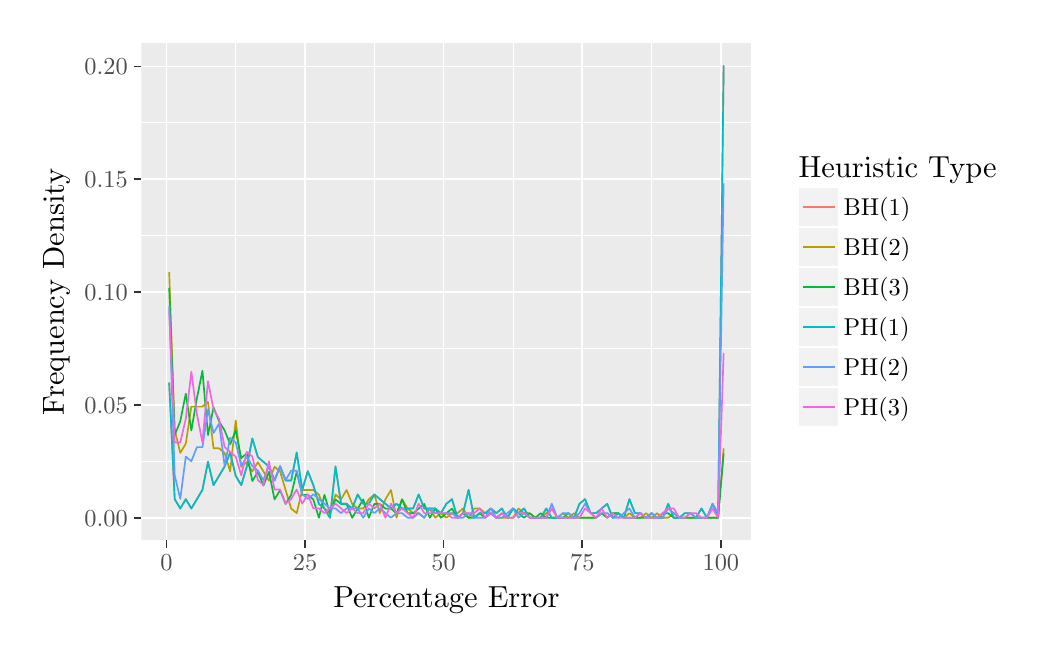
\begin{tikzpicture}[x=1pt,y=1pt]
\definecolor{fillColor}{RGB}{255,255,255}
\path[use as bounding box,fill=fillColor,fill opacity=0.00] (0,0) rectangle (361.35,216.81);
\begin{scope}
\path[clip] (  0.00,  0.00) rectangle (361.35,216.81);
\definecolor{drawColor}{RGB}{255,255,255}
\definecolor{fillColor}{RGB}{255,255,255}

\path[draw=drawColor,line width= 0.6pt,line join=round,line cap=round,fill=fillColor] (  0.00,  0.00) rectangle (361.35,216.81);
\end{scope}
\begin{scope}
\path[clip] ( 41.11, 31.53) rectangle (261.51,211.31);
\definecolor{fillColor}{gray}{0.92}

\path[fill=fillColor] ( 41.11, 31.53) rectangle (261.51,211.31);
\definecolor{drawColor}{RGB}{255,255,255}

\path[draw=drawColor,line width= 0.3pt,line join=round] ( 41.11, 60.09) --
	(261.51, 60.09);

\path[draw=drawColor,line width= 0.3pt,line join=round] ( 41.11,100.86) --
	(261.51,100.86);

\path[draw=drawColor,line width= 0.3pt,line join=round] ( 41.11,141.64) --
	(261.51,141.64);

\path[draw=drawColor,line width= 0.3pt,line join=round] ( 41.11,182.41) --
	(261.51,182.41);

\path[draw=drawColor,line width= 0.3pt,line join=round] ( 75.17, 31.53) --
	( 75.17,211.31);

\path[draw=drawColor,line width= 0.3pt,line join=round] (125.26, 31.53) --
	(125.26,211.31);

\path[draw=drawColor,line width= 0.3pt,line join=round] (175.36, 31.53) --
	(175.36,211.31);

\path[draw=drawColor,line width= 0.3pt,line join=round] (225.45, 31.53) --
	(225.45,211.31);

\path[draw=drawColor,line width= 0.6pt,line join=round] ( 41.11, 39.70) --
	(261.51, 39.70);

\path[draw=drawColor,line width= 0.6pt,line join=round] ( 41.11, 80.48) --
	(261.51, 80.48);

\path[draw=drawColor,line width= 0.6pt,line join=round] ( 41.11,121.25) --
	(261.51,121.25);

\path[draw=drawColor,line width= 0.6pt,line join=round] ( 41.11,162.03) --
	(261.51,162.03);

\path[draw=drawColor,line width= 0.6pt,line join=round] ( 41.11,202.80) --
	(261.51,202.80);

\path[draw=drawColor,line width= 0.6pt,line join=round] ( 50.13, 31.53) --
	( 50.13,211.31);

\path[draw=drawColor,line width= 0.6pt,line join=round] (100.22, 31.53) --
	(100.22,211.31);

\path[draw=drawColor,line width= 0.6pt,line join=round] (150.31, 31.53) --
	(150.31,211.31);

\path[draw=drawColor,line width= 0.6pt,line join=round] (200.40, 31.53) --
	(200.40,211.31);

\path[draw=drawColor,line width= 0.6pt,line join=round] (250.49, 31.53) --
	(250.49,211.31);
\definecolor{drawColor}{RGB}{248,118,109}

\path[draw=drawColor,line width= 0.6pt,line join=round] ( 51.13, 88.56) --
	( 53.13, 46.44) --
	( 55.14, 43.07) --
	( 57.14, 46.44) --
	( 59.14, 43.07) --
	( 61.15, 46.44) --
	( 63.15, 49.81) --
	( 65.15, 59.92) --
	( 67.16, 51.50) --
	( 69.16, 54.87) --
	( 71.17, 58.24) --
	( 73.17, 63.29) --
	( 75.17, 54.87) --
	( 77.18, 51.50) --
	( 79.18, 58.24) --
	( 81.18, 68.35) --
	( 83.19, 61.61) --
	( 85.19, 59.92) --
	( 87.19, 58.24) --
	( 89.20, 53.18) --
	( 91.20, 58.24) --
	( 93.21, 53.18) --
	( 95.21, 53.18) --
	( 97.21, 63.29) --
	( 99.22, 49.81) --
	(101.22, 56.55) --
	(103.22, 51.50) --
	(105.23, 44.76) --
	(107.23, 43.07) --
	(109.24, 39.70) --
	(111.24, 58.24) --
	(113.24, 44.76) --
	(115.25, 44.76) --
	(117.25, 43.07) --
	(119.25, 48.13) --
	(121.26, 44.76) --
	(123.26, 44.76) --
	(125.26, 48.13) --
	(127.27, 46.44) --
	(129.27, 44.76) --
	(131.28, 43.07) --
	(133.28, 44.76) --
	(135.28, 43.07) --
	(137.29, 43.07) --
	(139.29, 43.07) --
	(141.29, 48.13) --
	(143.30, 43.07) --
	(145.30, 43.07) --
	(147.30, 43.07) --
	(149.31, 41.39) --
	(151.31, 44.76) --
	(153.32, 46.44) --
	(155.32, 39.70) --
	(157.32, 41.39) --
	(159.33, 49.81) --
	(161.33, 39.70) --
	(163.33, 41.39) --
	(165.34, 41.39) --
	(167.34, 43.07) --
	(169.34, 41.39) --
	(171.35, 43.07) --
	(173.35, 39.70) --
	(175.36, 43.07) --
	(177.36, 41.39) --
	(179.36, 43.07) --
	(181.37, 39.70) --
	(183.37, 39.70) --
	(185.37, 39.70) --
	(187.38, 43.07) --
	(189.38, 39.70) --
	(191.39, 39.70) --
	(193.39, 39.70) --
	(195.39, 41.39) --
	(197.40, 39.70) --
	(199.40, 44.76) --
	(201.40, 46.44) --
	(203.41, 41.39) --
	(205.41, 41.39) --
	(207.41, 43.07) --
	(209.42, 44.76) --
	(211.42, 39.70) --
	(213.43, 41.39) --
	(215.43, 39.70) --
	(217.43, 46.44) --
	(219.44, 41.39) --
	(221.44, 41.39) --
	(223.44, 39.70) --
	(225.45, 41.39) --
	(227.45, 39.70) --
	(229.45, 39.70) --
	(231.46, 44.76) --
	(233.46, 39.70) --
	(235.47, 39.70) --
	(237.47, 41.39) --
	(239.47, 41.39) --
	(241.48, 39.70) --
	(243.48, 43.07) --
	(245.48, 39.70) --
	(247.49, 44.76) --
	(249.49, 39.70) --
	(251.49,203.14);
\definecolor{drawColor}{RGB}{183,159,0}

\path[draw=drawColor,line width= 0.6pt,line join=round] ( 51.13,128.45) --
	( 53.13, 71.52) --
	( 55.14, 63.15) --
	( 57.14, 66.49) --
	( 59.14, 79.89) --
	( 61.15, 79.89) --
	( 63.15, 79.89) --
	( 65.15, 81.57) --
	( 67.16, 64.82) --
	( 69.16, 64.82) --
	( 71.17, 63.15) --
	( 73.17, 56.45) --
	( 75.17, 74.87) --
	( 77.18, 58.12) --
	( 79.18, 59.80) --
	( 81.18, 56.45) --
	( 83.19, 59.80) --
	( 85.19, 56.45) --
	( 87.19, 53.10) --
	( 89.20, 58.12) --
	( 91.20, 56.45) --
	( 93.21, 49.75) --
	( 95.21, 43.05) --
	( 97.21, 41.38) --
	( 99.22, 49.75) --
	(101.22, 49.75) --
	(103.22, 49.75) --
	(105.23, 48.08) --
	(107.23, 43.05) --
	(109.24, 41.38) --
	(111.24, 48.08) --
	(113.24, 46.40) --
	(115.25, 49.75) --
	(117.25, 44.73) --
	(119.25, 43.05) --
	(121.26, 43.05) --
	(123.26, 46.40) --
	(125.26, 48.08) --
	(127.27, 41.38) --
	(129.27, 46.40) --
	(131.28, 49.75) --
	(133.28, 39.70) --
	(135.28, 46.40) --
	(137.29, 43.05) --
	(139.29, 41.38) --
	(141.29, 41.38) --
	(143.30, 39.70) --
	(145.30, 43.05) --
	(147.30, 39.70) --
	(149.31, 41.38) --
	(151.31, 39.70) --
	(153.32, 41.38) --
	(155.32, 41.38) --
	(157.32, 43.05) --
	(159.33, 39.70) --
	(161.33, 43.05) --
	(163.33, 43.05) --
	(165.34, 41.38) --
	(167.34, 41.38) --
	(169.34, 39.70) --
	(171.35, 39.70) --
	(173.35, 39.70) --
	(175.36, 39.70) --
	(177.36, 43.05) --
	(179.36, 41.38) --
	(181.37, 41.38) --
	(183.37, 39.70) --
	(185.37, 39.70) --
	(187.38, 41.38) --
	(189.38, 43.05) --
	(191.39, 39.70) --
	(193.39, 41.38) --
	(195.39, 39.70) --
	(197.40, 41.38) --
	(199.40, 39.70) --
	(201.40, 39.70) --
	(203.41, 39.70) --
	(205.41, 39.70) --
	(207.41, 41.38) --
	(209.42, 39.70) --
	(211.42, 41.38) --
	(213.43, 41.38) --
	(215.43, 39.70) --
	(217.43, 41.38) --
	(219.44, 39.70) --
	(221.44, 39.70) --
	(223.44, 41.38) --
	(225.45, 39.70) --
	(227.45, 41.38) --
	(229.45, 39.70) --
	(231.46, 39.70) --
	(233.46, 41.38) --
	(235.47, 39.70) --
	(237.47, 39.70) --
	(239.47, 39.70) --
	(241.48, 39.70) --
	(243.48, 39.70) --
	(245.48, 39.70) --
	(247.49, 39.70) --
	(249.49, 39.70) --
	(251.49, 64.82);
\definecolor{drawColor}{RGB}{0,186,56}

\path[draw=drawColor,line width= 0.6pt,line join=round] ( 51.13,122.75) --
	( 53.13, 69.60) --
	( 55.14, 74.58) --
	( 57.14, 84.55) --
	( 59.14, 71.26) --
	( 61.15, 82.89) --
	( 63.15, 92.85) --
	( 65.15, 69.60) --
	( 67.16, 79.56) --
	( 69.16, 74.58) --
	( 71.17, 71.26) --
	( 73.17, 66.28) --
	( 75.17, 71.26) --
	( 77.18, 61.29) --
	( 79.18, 62.95) --
	( 81.18, 52.99) --
	( 83.19, 56.31) --
	( 85.19, 51.33) --
	( 87.19, 56.31) --
	( 89.20, 46.35) --
	( 91.20, 49.67) --
	( 93.21, 44.69) --
	( 95.21, 48.01) --
	( 97.21, 56.31) --
	( 99.22, 48.01) --
	(101.22, 48.01) --
	(103.22, 46.35) --
	(105.23, 39.70) --
	(107.23, 48.01) --
	(109.24, 41.36) --
	(111.24, 46.35) --
	(113.24, 44.69) --
	(115.25, 44.69) --
	(117.25, 39.70) --
	(119.25, 43.02) --
	(121.26, 46.35) --
	(123.26, 39.70) --
	(125.26, 44.69) --
	(127.27, 44.69) --
	(129.27, 43.02) --
	(131.28, 43.02) --
	(133.28, 41.36) --
	(135.28, 46.35) --
	(137.29, 41.36) --
	(139.29, 41.36) --
	(141.29, 43.02) --
	(143.30, 44.69) --
	(145.30, 39.70) --
	(147.30, 43.02) --
	(149.31, 39.70) --
	(151.31, 41.36) --
	(153.32, 43.02) --
	(155.32, 39.70) --
	(157.32, 41.36) --
	(159.33, 39.70) --
	(161.33, 39.70) --
	(163.33, 41.36) --
	(165.34, 39.70) --
	(167.34, 41.36) --
	(169.34, 39.70) --
	(171.35, 41.36) --
	(173.35, 39.70) --
	(175.36, 43.02) --
	(177.36, 41.36) --
	(179.36, 39.70) --
	(181.37, 41.36) --
	(183.37, 39.70) --
	(185.37, 41.36) --
	(187.38, 39.70) --
	(189.38, 39.70) --
	(191.39, 39.70) --
	(193.39, 39.70) --
	(195.39, 39.70) --
	(197.40, 39.70) --
	(199.40, 39.70) --
	(201.40, 39.70) --
	(203.41, 39.70) --
	(205.41, 39.70) --
	(207.41, 41.36) --
	(209.42, 39.70) --
	(211.42, 41.36) --
	(213.43, 41.36) --
	(215.43, 39.70) --
	(217.43, 39.70) --
	(219.44, 39.70) --
	(221.44, 39.70) --
	(223.44, 39.70) --
	(225.45, 39.70) --
	(227.45, 39.70) --
	(229.45, 41.36) --
	(231.46, 41.36) --
	(233.46, 39.70) --
	(235.47, 39.70) --
	(237.47, 39.70) --
	(239.47, 39.70) --
	(241.48, 39.70) --
	(243.48, 39.70) --
	(245.48, 39.70) --
	(247.49, 39.70) --
	(249.49, 39.70) --
	(251.49, 62.95);
\definecolor{drawColor}{RGB}{0,191,196}

\path[draw=drawColor,line width= 0.6pt,line join=round] ( 51.13, 88.56) --
	( 53.13, 46.44) --
	( 55.14, 43.07) --
	( 57.14, 46.44) --
	( 59.14, 43.07) --
	( 61.15, 46.44) --
	( 63.15, 49.81) --
	( 65.15, 59.92) --
	( 67.16, 51.50) --
	( 69.16, 54.87) --
	( 71.17, 58.24) --
	( 73.17, 63.29) --
	( 75.17, 54.87) --
	( 77.18, 51.50) --
	( 79.18, 58.24) --
	( 81.18, 68.35) --
	( 83.19, 61.61) --
	( 85.19, 59.92) --
	( 87.19, 58.24) --
	( 89.20, 53.18) --
	( 91.20, 58.24) --
	( 93.21, 53.18) --
	( 95.21, 53.18) --
	( 97.21, 63.29) --
	( 99.22, 49.81) --
	(101.22, 56.55) --
	(103.22, 51.50) --
	(105.23, 44.76) --
	(107.23, 43.07) --
	(109.24, 39.70) --
	(111.24, 58.24) --
	(113.24, 44.76) --
	(115.25, 44.76) --
	(117.25, 43.07) --
	(119.25, 48.13) --
	(121.26, 44.76) --
	(123.26, 44.76) --
	(125.26, 48.13) --
	(127.27, 46.44) --
	(129.27, 44.76) --
	(131.28, 43.07) --
	(133.28, 44.76) --
	(135.28, 43.07) --
	(137.29, 43.07) --
	(139.29, 43.07) --
	(141.29, 48.13) --
	(143.30, 43.07) --
	(145.30, 43.07) --
	(147.30, 43.07) --
	(149.31, 41.39) --
	(151.31, 44.76) --
	(153.32, 46.44) --
	(155.32, 39.70) --
	(157.32, 41.39) --
	(159.33, 49.81) --
	(161.33, 39.70) --
	(163.33, 41.39) --
	(165.34, 41.39) --
	(167.34, 43.07) --
	(169.34, 41.39) --
	(171.35, 43.07) --
	(173.35, 39.70) --
	(175.36, 43.07) --
	(177.36, 41.39) --
	(179.36, 43.07) --
	(181.37, 39.70) --
	(183.37, 39.70) --
	(185.37, 39.70) --
	(187.38, 43.07) --
	(189.38, 39.70) --
	(191.39, 39.70) --
	(193.39, 39.70) --
	(195.39, 41.39) --
	(197.40, 39.70) --
	(199.40, 44.76) --
	(201.40, 46.44) --
	(203.41, 41.39) --
	(205.41, 41.39) --
	(207.41, 43.07) --
	(209.42, 44.76) --
	(211.42, 39.70) --
	(213.43, 41.39) --
	(215.43, 39.70) --
	(217.43, 46.44) --
	(219.44, 41.39) --
	(221.44, 41.39) --
	(223.44, 39.70) --
	(225.45, 41.39) --
	(227.45, 39.70) --
	(229.45, 39.70) --
	(231.46, 44.76) --
	(233.46, 39.70) --
	(235.47, 39.70) --
	(237.47, 41.39) --
	(239.47, 41.39) --
	(241.48, 39.70) --
	(243.48, 43.07) --
	(245.48, 39.70) --
	(247.49, 44.76) --
	(249.49, 39.70) --
	(251.49,203.14);
\definecolor{drawColor}{RGB}{97,156,255}

\path[draw=drawColor,line width= 0.6pt,line join=round] ( 51.13,116.31) --
	( 53.13, 55.02) --
	( 55.14, 46.51) --
	( 57.14, 61.83) --
	( 59.14, 60.13) --
	( 61.15, 65.24) --
	( 63.15, 65.24) --
	( 65.15, 78.86) --
	( 67.16, 70.35) --
	( 69.16, 73.75) --
	( 71.17, 58.43) --
	( 73.17, 68.64) --
	( 75.17, 66.94) --
	( 77.18, 58.43) --
	( 79.18, 61.83) --
	( 81.18, 58.43) --
	( 83.19, 56.73) --
	( 85.19, 53.32) --
	( 87.19, 58.43) --
	( 89.20, 53.32) --
	( 91.20, 58.43) --
	( 93.21, 53.32) --
	( 95.21, 56.73) --
	( 97.21, 56.73) --
	( 99.22, 48.21) --
	(101.22, 46.51) --
	(103.22, 48.21) --
	(105.23, 46.51) --
	(107.23, 44.81) --
	(109.24, 43.11) --
	(111.24, 43.11) --
	(113.24, 41.40) --
	(115.25, 43.11) --
	(117.25, 43.11) --
	(119.25, 43.11) --
	(121.26, 39.70) --
	(123.26, 43.11) --
	(125.26, 41.40) --
	(127.27, 43.11) --
	(129.27, 41.40) --
	(131.28, 39.70) --
	(133.28, 41.40) --
	(135.28, 41.40) --
	(137.29, 39.70) --
	(139.29, 39.70) --
	(141.29, 41.40) --
	(143.30, 39.70) --
	(145.30, 43.11) --
	(147.30, 41.40) --
	(149.31, 41.40) --
	(151.31, 41.40) --
	(153.32, 41.40) --
	(155.32, 39.70) --
	(157.32, 39.70) --
	(159.33, 41.40) --
	(161.33, 39.70) --
	(163.33, 39.70) --
	(165.34, 39.70) --
	(167.34, 43.11) --
	(169.34, 39.70) --
	(171.35, 39.70) --
	(173.35, 41.40) --
	(175.36, 43.11) --
	(177.36, 39.70) --
	(179.36, 41.40) --
	(181.37, 39.70) --
	(183.37, 39.70) --
	(185.37, 39.70) --
	(187.38, 39.70) --
	(189.38, 44.81) --
	(191.39, 39.70) --
	(193.39, 41.40) --
	(195.39, 41.40) --
	(197.40, 39.70) --
	(199.40, 41.40) --
	(201.40, 44.81) --
	(203.41, 41.40) --
	(205.41, 39.70) --
	(207.41, 41.40) --
	(209.42, 41.40) --
	(211.42, 39.70) --
	(213.43, 39.70) --
	(215.43, 41.40) --
	(217.43, 43.11) --
	(219.44, 39.70) --
	(221.44, 41.40) --
	(223.44, 39.70) --
	(225.45, 41.40) --
	(227.45, 39.70) --
	(229.45, 39.70) --
	(231.46, 43.11) --
	(233.46, 41.40) --
	(235.47, 39.70) --
	(237.47, 39.70) --
	(239.47, 41.40) --
	(241.48, 39.70) --
	(243.48, 39.70) --
	(245.48, 39.70) --
	(247.49, 44.81) --
	(249.49, 41.40) --
	(251.49,160.58);
\definecolor{drawColor}{RGB}{245,100,227}

\path[draw=drawColor,line width= 0.6pt,line join=round] ( 51.13,114.61) --
	( 53.13, 66.94) --
	( 55.14, 66.94) --
	( 57.14, 75.45) --
	( 59.14, 92.48) --
	( 61.15, 77.16) --
	( 63.15, 66.94) --
	( 65.15, 89.07) --
	( 67.16, 78.86) --
	( 69.16, 75.45) --
	( 71.17, 65.24) --
	( 73.17, 63.54) --
	( 75.17, 61.83) --
	( 77.18, 55.02) --
	( 79.18, 63.54) --
	( 81.18, 61.83) --
	( 83.19, 53.32) --
	( 85.19, 51.62) --
	( 87.19, 60.13) --
	( 89.20, 49.92) --
	( 91.20, 49.92) --
	( 93.21, 44.81) --
	( 95.21, 46.51) --
	( 97.21, 49.92) --
	( 99.22, 44.81) --
	(101.22, 48.21) --
	(103.22, 43.11) --
	(105.23, 43.11) --
	(107.23, 41.40) --
	(109.24, 43.11) --
	(111.24, 44.81) --
	(113.24, 43.11) --
	(115.25, 41.40) --
	(117.25, 43.11) --
	(119.25, 41.40) --
	(121.26, 41.40) --
	(123.26, 44.81) --
	(125.26, 43.11) --
	(127.27, 44.81) --
	(129.27, 39.70) --
	(131.28, 44.81) --
	(133.28, 41.40) --
	(135.28, 43.11) --
	(137.29, 41.40) --
	(139.29, 39.70) --
	(141.29, 44.81) --
	(143.30, 41.40) --
	(145.30, 41.40) --
	(147.30, 41.40) --
	(149.31, 41.40) --
	(151.31, 41.40) --
	(153.32, 39.70) --
	(155.32, 39.70) --
	(157.32, 41.40) --
	(159.33, 41.40) --
	(161.33, 41.40) --
	(163.33, 43.11) --
	(165.34, 39.70) --
	(167.34, 41.40) --
	(169.34, 39.70) --
	(171.35, 41.40) --
	(173.35, 39.70) --
	(175.36, 39.70) --
	(177.36, 41.40) --
	(179.36, 41.40) --
	(181.37, 39.70) --
	(183.37, 39.70) --
	(185.37, 39.70) --
	(187.38, 39.70) --
	(189.38, 43.11) --
	(191.39, 39.70) --
	(193.39, 39.70) --
	(195.39, 39.70) --
	(197.40, 39.70) --
	(199.40, 39.70) --
	(201.40, 43.11) --
	(203.41, 41.40) --
	(205.41, 39.70) --
	(207.41, 43.11) --
	(209.42, 39.70) --
	(211.42, 41.40) --
	(213.43, 39.70) --
	(215.43, 39.70) --
	(217.43, 39.70) --
	(219.44, 39.70) --
	(221.44, 41.40) --
	(223.44, 39.70) --
	(225.45, 39.70) --
	(227.45, 39.70) --
	(229.45, 41.40) --
	(231.46, 43.11) --
	(233.46, 43.11) --
	(235.47, 39.70) --
	(237.47, 39.70) --
	(239.47, 41.40) --
	(241.48, 41.40) --
	(243.48, 39.70) --
	(245.48, 39.70) --
	(247.49, 43.11) --
	(249.49, 39.70) --
	(251.49, 99.29);
\end{scope}
\begin{scope}
\path[clip] (  0.00,  0.00) rectangle (361.35,216.81);
\definecolor{drawColor}{gray}{0.30}

\node[text=drawColor,anchor=base east,inner sep=0pt, outer sep=0pt, scale=  0.88] at ( 36.16, 36.67) {0.00};

\node[text=drawColor,anchor=base east,inner sep=0pt, outer sep=0pt, scale=  0.88] at ( 36.16, 77.45) {0.05};

\node[text=drawColor,anchor=base east,inner sep=0pt, outer sep=0pt, scale=  0.88] at ( 36.16,118.22) {0.10};

\node[text=drawColor,anchor=base east,inner sep=0pt, outer sep=0pt, scale=  0.88] at ( 36.16,159.00) {0.15};

\node[text=drawColor,anchor=base east,inner sep=0pt, outer sep=0pt, scale=  0.88] at ( 36.16,199.77) {0.20};
\end{scope}
\begin{scope}
\path[clip] (  0.00,  0.00) rectangle (361.35,216.81);
\definecolor{drawColor}{gray}{0.20}

\path[draw=drawColor,line width= 0.6pt,line join=round] ( 38.36, 39.70) --
	( 41.11, 39.70);

\path[draw=drawColor,line width= 0.6pt,line join=round] ( 38.36, 80.48) --
	( 41.11, 80.48);

\path[draw=drawColor,line width= 0.6pt,line join=round] ( 38.36,121.25) --
	( 41.11,121.25);

\path[draw=drawColor,line width= 0.6pt,line join=round] ( 38.36,162.03) --
	( 41.11,162.03);

\path[draw=drawColor,line width= 0.6pt,line join=round] ( 38.36,202.80) --
	( 41.11,202.80);
\end{scope}
\begin{scope}
\path[clip] (  0.00,  0.00) rectangle (361.35,216.81);
\definecolor{drawColor}{gray}{0.20}

\path[draw=drawColor,line width= 0.6pt,line join=round] ( 50.13, 28.78) --
	( 50.13, 31.53);

\path[draw=drawColor,line width= 0.6pt,line join=round] (100.22, 28.78) --
	(100.22, 31.53);

\path[draw=drawColor,line width= 0.6pt,line join=round] (150.31, 28.78) --
	(150.31, 31.53);

\path[draw=drawColor,line width= 0.6pt,line join=round] (200.40, 28.78) --
	(200.40, 31.53);

\path[draw=drawColor,line width= 0.6pt,line join=round] (250.49, 28.78) --
	(250.49, 31.53);
\end{scope}
\begin{scope}
\path[clip] (  0.00,  0.00) rectangle (361.35,216.81);
\definecolor{drawColor}{gray}{0.30}

\node[text=drawColor,anchor=base,inner sep=0pt, outer sep=0pt, scale=  0.88] at ( 50.13, 20.52) {0};

\node[text=drawColor,anchor=base,inner sep=0pt, outer sep=0pt, scale=  0.88] at (100.22, 20.52) {25};

\node[text=drawColor,anchor=base,inner sep=0pt, outer sep=0pt, scale=  0.88] at (150.31, 20.52) {50};

\node[text=drawColor,anchor=base,inner sep=0pt, outer sep=0pt, scale=  0.88] at (200.40, 20.52) {75};

\node[text=drawColor,anchor=base,inner sep=0pt, outer sep=0pt, scale=  0.88] at (250.49, 20.52) {100};
\end{scope}
\begin{scope}
\path[clip] (  0.00,  0.00) rectangle (361.35,216.81);
\definecolor{drawColor}{RGB}{0,0,0}

\node[text=drawColor,anchor=base,inner sep=0pt, outer sep=0pt, scale=  1.10] at (151.31,  7.44) {Percentage Error};
\end{scope}
\begin{scope}
\path[clip] (  0.00,  0.00) rectangle (361.35,216.81);
\definecolor{drawColor}{RGB}{0,0,0}

\node[text=drawColor,rotate= 90.00,anchor=base,inner sep=0pt, outer sep=0pt, scale=  1.10] at ( 13.08,121.42) {Frequency Density};
\end{scope}
\begin{scope}
\path[clip] (  0.00,  0.00) rectangle (361.35,216.81);
\definecolor{fillColor}{RGB}{255,255,255}

\path[fill=fillColor] (272.89, 66.77) rectangle (355.85,176.07);
\end{scope}
\begin{scope}
\path[clip] (  0.00,  0.00) rectangle (361.35,216.81);
\definecolor{drawColor}{RGB}{0,0,0}

\node[text=drawColor,anchor=base west,inner sep=0pt, outer sep=0pt, scale=  1.10] at (278.58,162.80) {Heuristic Type};
\end{scope}
\begin{scope}
\path[clip] (  0.00,  0.00) rectangle (361.35,216.81);
\definecolor{drawColor}{RGB}{255,255,255}
\definecolor{fillColor}{gray}{0.95}

\path[draw=drawColor,line width= 0.6pt,line join=round,line cap=round,fill=fillColor] (278.58,144.73) rectangle (293.04,159.19);
\end{scope}
\begin{scope}
\path[clip] (  0.00,  0.00) rectangle (361.35,216.81);
\definecolor{drawColor}{RGB}{248,118,109}

\path[draw=drawColor,line width= 0.6pt,line join=round] (280.03,151.96) -- (291.59,151.96);
\end{scope}
\begin{scope}
\path[clip] (  0.00,  0.00) rectangle (361.35,216.81);
\definecolor{drawColor}{RGB}{255,255,255}
\definecolor{fillColor}{gray}{0.95}

\path[draw=drawColor,line width= 0.6pt,line join=round,line cap=round,fill=fillColor] (278.58,130.28) rectangle (293.04,144.73);
\end{scope}
\begin{scope}
\path[clip] (  0.00,  0.00) rectangle (361.35,216.81);
\definecolor{drawColor}{RGB}{183,159,0}

\path[draw=drawColor,line width= 0.6pt,line join=round] (280.03,137.51) -- (291.59,137.51);
\end{scope}
\begin{scope}
\path[clip] (  0.00,  0.00) rectangle (361.35,216.81);
\definecolor{drawColor}{RGB}{255,255,255}
\definecolor{fillColor}{gray}{0.95}

\path[draw=drawColor,line width= 0.6pt,line join=round,line cap=round,fill=fillColor] (278.58,115.83) rectangle (293.04,130.28);
\end{scope}
\begin{scope}
\path[clip] (  0.00,  0.00) rectangle (361.35,216.81);
\definecolor{drawColor}{RGB}{0,186,56}

\path[draw=drawColor,line width= 0.6pt,line join=round] (280.03,123.05) -- (291.59,123.05);
\end{scope}
\begin{scope}
\path[clip] (  0.00,  0.00) rectangle (361.35,216.81);
\definecolor{drawColor}{RGB}{255,255,255}
\definecolor{fillColor}{gray}{0.95}

\path[draw=drawColor,line width= 0.6pt,line join=round,line cap=round,fill=fillColor] (278.58,101.37) rectangle (293.04,115.83);
\end{scope}
\begin{scope}
\path[clip] (  0.00,  0.00) rectangle (361.35,216.81);
\definecolor{drawColor}{RGB}{0,191,196}

\path[draw=drawColor,line width= 0.6pt,line join=round] (280.03,108.60) -- (291.59,108.60);
\end{scope}
\begin{scope}
\path[clip] (  0.00,  0.00) rectangle (361.35,216.81);
\definecolor{drawColor}{RGB}{255,255,255}
\definecolor{fillColor}{gray}{0.95}

\path[draw=drawColor,line width= 0.6pt,line join=round,line cap=round,fill=fillColor] (278.58, 86.92) rectangle (293.04,101.37);
\end{scope}
\begin{scope}
\path[clip] (  0.00,  0.00) rectangle (361.35,216.81);
\definecolor{drawColor}{RGB}{97,156,255}

\path[draw=drawColor,line width= 0.6pt,line join=round] (280.03, 94.14) -- (291.59, 94.14);
\end{scope}
\begin{scope}
\path[clip] (  0.00,  0.00) rectangle (361.35,216.81);
\definecolor{drawColor}{RGB}{255,255,255}
\definecolor{fillColor}{gray}{0.95}

\path[draw=drawColor,line width= 0.6pt,line join=round,line cap=round,fill=fillColor] (278.58, 72.46) rectangle (293.04, 86.92);
\end{scope}
\begin{scope}
\path[clip] (  0.00,  0.00) rectangle (361.35,216.81);
\definecolor{drawColor}{RGB}{245,100,227}

\path[draw=drawColor,line width= 0.6pt,line join=round] (280.03, 79.69) -- (291.59, 79.69);
\end{scope}
\begin{scope}
\path[clip] (  0.00,  0.00) rectangle (361.35,216.81);
\definecolor{drawColor}{RGB}{0,0,0}

\node[text=drawColor,anchor=base west,inner sep=0pt, outer sep=0pt, scale=  0.88] at (294.85,148.93) {BH($1$)};
\end{scope}
\begin{scope}
\path[clip] (  0.00,  0.00) rectangle (361.35,216.81);
\definecolor{drawColor}{RGB}{0,0,0}

\node[text=drawColor,anchor=base west,inner sep=0pt, outer sep=0pt, scale=  0.88] at (294.85,134.48) {BH($2$)};
\end{scope}
\begin{scope}
\path[clip] (  0.00,  0.00) rectangle (361.35,216.81);
\definecolor{drawColor}{RGB}{0,0,0}

\node[text=drawColor,anchor=base west,inner sep=0pt, outer sep=0pt, scale=  0.88] at (294.85,120.02) {BH($3$)};
\end{scope}
\begin{scope}
\path[clip] (  0.00,  0.00) rectangle (361.35,216.81);
\definecolor{drawColor}{RGB}{0,0,0}

\node[text=drawColor,anchor=base west,inner sep=0pt, outer sep=0pt, scale=  0.88] at (294.85,105.57) {PH($1$)};
\end{scope}
\begin{scope}
\path[clip] (  0.00,  0.00) rectangle (361.35,216.81);
\definecolor{drawColor}{RGB}{0,0,0}

\node[text=drawColor,anchor=base west,inner sep=0pt, outer sep=0pt, scale=  0.88] at (294.85, 91.11) {PH($2$)};
\end{scope}
\begin{scope}
\path[clip] (  0.00,  0.00) rectangle (361.35,216.81);
\definecolor{drawColor}{RGB}{0,0,0}

\node[text=drawColor,anchor=base west,inner sep=0pt, outer sep=0pt, scale=  0.88] at (294.85, 76.66) {PH($3$)};
\end{scope}
\end{tikzpicture}

\caption{Frequency density of percentage errors made by heuristics in simulations.}
\label{Figure:Initial RH and PH for plain index}
\end{myfigure}

From Figure \ref{Figure:Initial RH and PH for plain index} we can see that while sometimes the heuristic performs well, in the majority of cases it performs very badly.

We propose altering the index to,

\begin{align}
W_{i}(s_{i},v_{i})&=\begin{cases}
0 \text{ If } s_{i}<B_{i} \\
\Delta_{i}(v_{i}) \text{ If } s_{i}=B_{i} \\
\Delta_{i}(v_{i}+1) \text{ If } s_{i}=B_{i}+1 , v_{i} < v_{i,\text{max}} \\
\widetilde{\Delta_{i}} \text{ If } s_{i}=B_{i}+1, v_{i} \geq v_{i,\text{max}} \\
\end{cases}
\end{align}
and run the same scenarios with our changed index.

\begin{myfigure}
% Created by tikzDevice version 0.10.1 on 2018-06-12 12:28:58
% !TEX encoding = UTF-8 Unicode
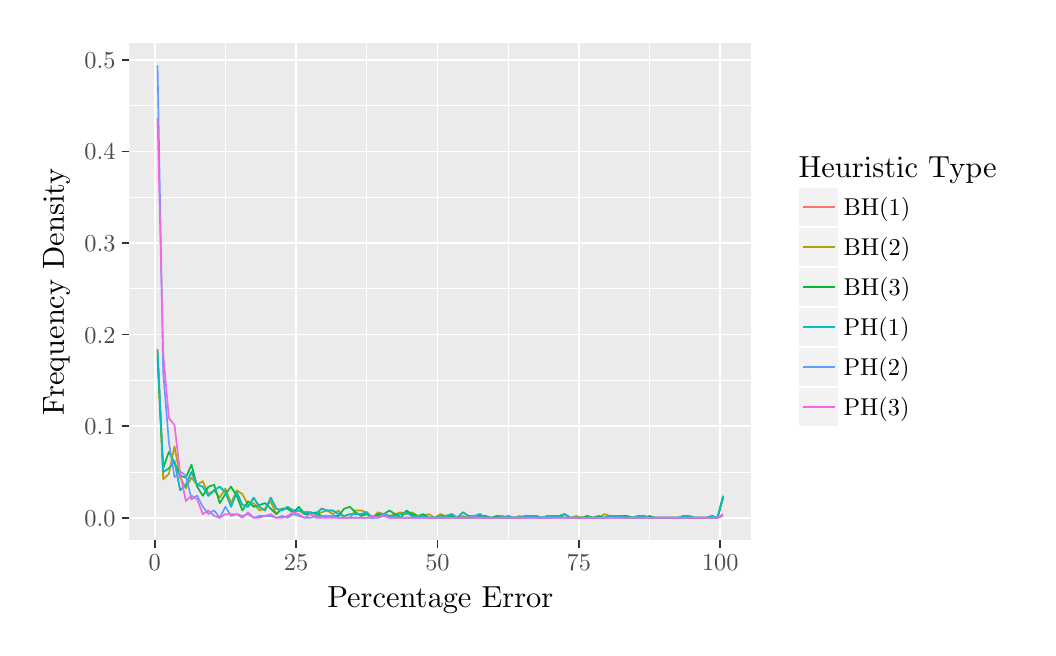
\begin{tikzpicture}[x=1pt,y=1pt]
\definecolor{fillColor}{RGB}{255,255,255}
\path[use as bounding box,fill=fillColor,fill opacity=0.00] (0,0) rectangle (361.35,216.81);
\begin{scope}
\path[clip] (  0.00,  0.00) rectangle (361.35,216.81);
\definecolor{drawColor}{RGB}{255,255,255}
\definecolor{fillColor}{RGB}{255,255,255}

\path[draw=drawColor,line width= 0.6pt,line join=round,line cap=round,fill=fillColor] (  0.00,  0.00) rectangle (361.35,216.81);
\end{scope}
\begin{scope}
\path[clip] ( 36.71, 31.53) rectangle (261.51,211.31);
\definecolor{fillColor}{gray}{0.92}

\path[fill=fillColor] ( 36.71, 31.53) rectangle (261.51,211.31);
\definecolor{drawColor}{RGB}{255,255,255}

\path[draw=drawColor,line width= 0.3pt,line join=round] ( 36.71, 56.25) --
	(261.51, 56.25);

\path[draw=drawColor,line width= 0.3pt,line join=round] ( 36.71, 89.33) --
	(261.51, 89.33);

\path[draw=drawColor,line width= 0.3pt,line join=round] ( 36.71,122.42) --
	(261.51,122.42);

\path[draw=drawColor,line width= 0.3pt,line join=round] ( 36.71,155.51) --
	(261.51,155.51);

\path[draw=drawColor,line width= 0.3pt,line join=round] ( 36.71,188.60) --
	(261.51,188.60);

\path[draw=drawColor,line width= 0.3pt,line join=round] ( 71.45, 31.53) --
	( 71.45,211.31);

\path[draw=drawColor,line width= 0.3pt,line join=round] (122.54, 31.53) --
	(122.54,211.31);

\path[draw=drawColor,line width= 0.3pt,line join=round] (173.64, 31.53) --
	(173.64,211.31);

\path[draw=drawColor,line width= 0.3pt,line join=round] (224.73, 31.53) --
	(224.73,211.31);

\path[draw=drawColor,line width= 0.6pt,line join=round] ( 36.71, 39.70) --
	(261.51, 39.70);

\path[draw=drawColor,line width= 0.6pt,line join=round] ( 36.71, 72.79) --
	(261.51, 72.79);

\path[draw=drawColor,line width= 0.6pt,line join=round] ( 36.71,105.88) --
	(261.51,105.88);

\path[draw=drawColor,line width= 0.6pt,line join=round] ( 36.71,138.96) --
	(261.51,138.96);

\path[draw=drawColor,line width= 0.6pt,line join=round] ( 36.71,172.05) --
	(261.51,172.05);

\path[draw=drawColor,line width= 0.6pt,line join=round] ( 36.71,205.14) --
	(261.51,205.14);

\path[draw=drawColor,line width= 0.6pt,line join=round] ( 45.91, 31.53) --
	( 45.91,211.31);

\path[draw=drawColor,line width= 0.6pt,line join=round] ( 97.00, 31.53) --
	( 97.00,211.31);

\path[draw=drawColor,line width= 0.6pt,line join=round] (148.09, 31.53) --
	(148.09,211.31);

\path[draw=drawColor,line width= 0.6pt,line join=round] (199.18, 31.53) --
	(199.18,211.31);

\path[draw=drawColor,line width= 0.6pt,line join=round] (250.27, 31.53) --
	(250.27,211.31);
\definecolor{drawColor}{RGB}{248,118,109}

\path[draw=drawColor,line width= 0.6pt,line join=round] ( 46.93,100.58) --
	( 48.97, 56.25) --
	( 51.02, 57.57) --
	( 53.06, 60.22) --
	( 55.10, 49.63) --
	( 57.15, 51.61) --
	( 59.19, 56.25) --
	( 61.24, 51.61) --
	( 63.28, 50.95) --
	( 65.32, 47.64) --
	( 67.37, 49.63) --
	( 69.41, 50.95) --
	( 71.45, 48.97) --
	( 73.50, 43.67) --
	( 75.54, 48.97) --
	( 77.58, 44.33) --
	( 79.63, 43.67) --
	( 81.67, 46.98) --
	( 83.72, 43.67) --
	( 85.76, 42.35) --
	( 87.80, 46.98) --
	( 89.85, 43.01) --
	( 91.89, 42.35) --
	( 93.93, 43.67) --
	( 95.98, 42.35) --
	( 98.02, 42.35) --
	(100.06, 41.69) --
	(102.11, 41.69) --
	(104.15, 41.03) --
	(106.20, 43.01) --
	(108.24, 42.35) --
	(110.28, 42.35) --
	(112.33, 41.03) --
	(114.37, 40.36) --
	(116.41, 41.03) --
	(118.46, 41.03) --
	(120.50, 41.03) --
	(122.54, 41.69) --
	(124.59, 39.70) --
	(126.63, 40.36) --
	(128.68, 41.03) --
	(130.72, 40.36) --
	(132.76, 40.36) --
	(134.81, 41.03) --
	(136.85, 41.69) --
	(138.89, 40.36) --
	(140.94, 40.36) --
	(142.98, 40.36) --
	(145.03, 39.70) --
	(147.07, 39.70) --
	(149.11, 40.36) --
	(151.16, 40.36) --
	(153.20, 41.03) --
	(155.24, 39.70) --
	(157.29, 41.69) --
	(159.33, 40.36) --
	(161.37, 40.36) --
	(163.42, 41.03) --
	(165.46, 39.70) --
	(167.51, 39.70) --
	(169.55, 39.70) --
	(171.59, 39.70) --
	(173.64, 40.36) --
	(175.68, 39.70) --
	(177.72, 39.70) --
	(179.77, 40.36) --
	(181.81, 40.36) --
	(183.85, 40.36) --
	(185.90, 39.70) --
	(187.94, 40.36) --
	(189.99, 40.36) --
	(192.03, 40.36) --
	(194.07, 41.03) --
	(196.12, 39.70) --
	(198.16, 39.70) --
	(200.20, 39.70) --
	(202.25, 39.70) --
	(204.29, 39.70) --
	(206.33, 39.70) --
	(208.38, 39.70) --
	(210.42, 40.36) --
	(212.47, 40.36) --
	(214.51, 40.36) --
	(216.55, 39.70) --
	(218.60, 39.70) --
	(220.64, 40.36) --
	(222.68, 40.36) --
	(224.73, 39.70) --
	(226.77, 39.70) --
	(228.81, 39.70) --
	(230.86, 39.70) --
	(232.90, 39.70) --
	(234.95, 39.70) --
	(236.99, 40.36) --
	(239.03, 40.36) --
	(241.08, 39.70) --
	(243.12, 39.70) --
	(245.16, 39.70) --
	(247.21, 40.36) --
	(249.25, 39.70) --
	(251.29, 47.64);
\definecolor{drawColor}{RGB}{183,159,0}

\path[draw=drawColor,line width= 0.6pt,line join=round] ( 46.93, 98.60) --
	( 48.97, 53.60) --
	( 51.02, 55.58) --
	( 53.06, 65.51) --
	( 55.10, 54.26) --
	( 57.15, 50.29) --
	( 59.19, 54.26) --
	( 61.24, 51.61) --
	( 63.28, 52.94) --
	( 65.32, 48.31) --
	( 67.37, 49.63) --
	( 69.41, 46.98) --
	( 71.45, 50.29) --
	( 73.50, 45.00) --
	( 75.54, 49.63) --
	( 77.58, 48.31) --
	( 79.63, 44.33) --
	( 81.67, 45.00) --
	( 83.72, 42.35) --
	( 85.76, 43.01) --
	( 87.80, 45.66) --
	( 89.85, 41.03) --
	( 91.89, 43.01) --
	( 93.93, 43.01) --
	( 95.98, 41.69) --
	( 98.02, 42.35) --
	(100.06, 41.03) --
	(102.11, 41.69) --
	(104.15, 41.03) --
	(106.20, 41.69) --
	(108.24, 42.35) --
	(110.28, 41.03) --
	(112.33, 42.35) --
	(114.37, 39.70) --
	(116.41, 39.70) --
	(118.46, 42.35) --
	(120.50, 42.35) --
	(122.54, 41.69) --
	(124.59, 39.70) --
	(126.63, 41.69) --
	(128.68, 41.03) --
	(130.72, 40.36) --
	(132.76, 41.03) --
	(134.81, 41.69) --
	(136.85, 41.03) --
	(138.89, 41.69) --
	(140.94, 40.36) --
	(142.98, 40.36) --
	(145.03, 41.03) --
	(147.07, 39.70) --
	(149.11, 41.03) --
	(151.16, 40.36) --
	(153.20, 41.03) --
	(155.24, 39.70) --
	(157.29, 40.36) --
	(159.33, 39.70) --
	(161.37, 39.70) --
	(163.42, 39.70) --
	(165.46, 39.70) --
	(167.51, 39.70) --
	(169.55, 40.36) --
	(171.59, 40.36) --
	(173.64, 39.70) --
	(175.68, 39.70) --
	(177.72, 40.36) --
	(179.77, 39.70) --
	(181.81, 40.36) --
	(183.85, 39.70) --
	(185.90, 39.70) --
	(187.94, 40.36) --
	(189.99, 40.36) --
	(192.03, 39.70) --
	(194.07, 41.03) --
	(196.12, 39.70) --
	(198.16, 40.36) --
	(200.20, 39.70) --
	(202.25, 40.36) --
	(204.29, 39.70) --
	(206.33, 39.70) --
	(208.38, 41.03) --
	(210.42, 40.36) --
	(212.47, 40.36) --
	(214.51, 39.70) --
	(216.55, 39.70) --
	(218.60, 39.70) --
	(220.64, 40.36) --
	(222.68, 40.36) --
	(224.73, 39.70) --
	(226.77, 39.70) --
	(228.81, 39.70) --
	(230.86, 39.70) --
	(232.90, 39.70) --
	(234.95, 39.70) --
	(236.99, 40.36) --
	(239.03, 39.70) --
	(241.08, 39.70) --
	(243.12, 39.70) --
	(245.16, 39.70) --
	(247.21, 40.36) --
	(249.25, 39.70) --
	(251.29, 46.98);
\definecolor{drawColor}{RGB}{0,186,56}

\path[draw=drawColor,line width= 0.6pt,line join=round] ( 46.93, 97.27) --
	( 48.97, 57.57) --
	( 51.02, 63.53) --
	( 53.06, 59.55) --
	( 55.10, 54.92) --
	( 57.15, 54.26) --
	( 59.19, 58.89) --
	( 61.24, 50.95) --
	( 63.28, 47.64) --
	( 65.32, 50.95) --
	( 67.37, 51.61) --
	( 69.41, 45.00) --
	( 71.45, 48.31) --
	( 73.50, 50.95) --
	( 75.54, 47.64) --
	( 77.58, 42.35) --
	( 79.63, 45.66) --
	( 81.67, 43.67) --
	( 83.72, 44.33) --
	( 85.76, 45.00) --
	( 87.80, 43.01) --
	( 89.85, 41.03) --
	( 91.89, 43.01) --
	( 93.93, 43.01) --
	( 95.98, 41.69) --
	( 98.02, 43.67) --
	(100.06, 41.03) --
	(102.11, 41.03) --
	(104.15, 41.69) --
	(106.20, 40.36) --
	(108.24, 40.36) --
	(110.28, 40.36) --
	(112.33, 40.36) --
	(114.37, 43.01) --
	(116.41, 43.67) --
	(118.46, 41.69) --
	(120.50, 40.36) --
	(122.54, 41.03) --
	(124.59, 39.70) --
	(126.63, 41.03) --
	(128.68, 41.03) --
	(130.72, 42.35) --
	(132.76, 41.03) --
	(134.81, 39.70) --
	(136.85, 42.35) --
	(138.89, 41.03) --
	(140.94, 40.36) --
	(142.98, 41.03) --
	(145.03, 39.70) --
	(147.07, 39.70) --
	(149.11, 39.70) --
	(151.16, 39.70) --
	(153.20, 40.36) --
	(155.24, 39.70) --
	(157.29, 39.70) --
	(159.33, 39.70) --
	(161.37, 39.70) --
	(163.42, 40.36) --
	(165.46, 40.36) --
	(167.51, 39.70) --
	(169.55, 40.36) --
	(171.59, 39.70) --
	(173.64, 39.70) --
	(175.68, 39.70) --
	(177.72, 39.70) --
	(179.77, 40.36) --
	(181.81, 40.36) --
	(183.85, 39.70) --
	(185.90, 39.70) --
	(187.94, 39.70) --
	(189.99, 40.36) --
	(192.03, 40.36) --
	(194.07, 39.70) --
	(196.12, 39.70) --
	(198.16, 39.70) --
	(200.20, 39.70) --
	(202.25, 40.36) --
	(204.29, 39.70) --
	(206.33, 40.36) --
	(208.38, 39.70) --
	(210.42, 40.36) --
	(212.47, 39.70) --
	(214.51, 40.36) --
	(216.55, 40.36) --
	(218.60, 39.70) --
	(220.64, 39.70) --
	(222.68, 39.70) --
	(224.73, 40.36) --
	(226.77, 39.70) --
	(228.81, 39.70) --
	(230.86, 39.70) --
	(232.90, 39.70) --
	(234.95, 39.70) --
	(236.99, 39.70) --
	(239.03, 39.70) --
	(241.08, 39.70) --
	(243.12, 39.70) --
	(245.16, 39.70) --
	(247.21, 39.70) --
	(249.25, 39.70) --
	(251.29, 46.98);
\definecolor{drawColor}{RGB}{0,191,196}

\path[draw=drawColor,line width= 0.6pt,line join=round] ( 46.93,100.58) --
	( 48.97, 56.25) --
	( 51.02, 57.57) --
	( 53.06, 60.22) --
	( 55.10, 49.63) --
	( 57.15, 51.61) --
	( 59.19, 56.25) --
	( 61.24, 51.61) --
	( 63.28, 50.95) --
	( 65.32, 47.64) --
	( 67.37, 49.63) --
	( 69.41, 50.95) --
	( 71.45, 48.97) --
	( 73.50, 43.67) --
	( 75.54, 48.97) --
	( 77.58, 44.33) --
	( 79.63, 43.67) --
	( 81.67, 46.98) --
	( 83.72, 43.67) --
	( 85.76, 42.35) --
	( 87.80, 46.98) --
	( 89.85, 43.01) --
	( 91.89, 42.35) --
	( 93.93, 43.67) --
	( 95.98, 42.35) --
	( 98.02, 42.35) --
	(100.06, 41.69) --
	(102.11, 41.69) --
	(104.15, 41.03) --
	(106.20, 43.01) --
	(108.24, 42.35) --
	(110.28, 42.35) --
	(112.33, 41.03) --
	(114.37, 40.36) --
	(116.41, 41.03) --
	(118.46, 41.03) --
	(120.50, 41.03) --
	(122.54, 41.69) --
	(124.59, 39.70) --
	(126.63, 40.36) --
	(128.68, 41.03) --
	(130.72, 40.36) --
	(132.76, 40.36) --
	(134.81, 41.03) --
	(136.85, 41.69) --
	(138.89, 40.36) --
	(140.94, 40.36) --
	(142.98, 40.36) --
	(145.03, 39.70) --
	(147.07, 39.70) --
	(149.11, 40.36) --
	(151.16, 40.36) --
	(153.20, 41.03) --
	(155.24, 39.70) --
	(157.29, 41.69) --
	(159.33, 40.36) --
	(161.37, 40.36) --
	(163.42, 41.03) --
	(165.46, 39.70) --
	(167.51, 39.70) --
	(169.55, 39.70) --
	(171.59, 39.70) --
	(173.64, 40.36) --
	(175.68, 39.70) --
	(177.72, 39.70) --
	(179.77, 40.36) --
	(181.81, 40.36) --
	(183.85, 40.36) --
	(185.90, 39.70) --
	(187.94, 40.36) --
	(189.99, 40.36) --
	(192.03, 40.36) --
	(194.07, 41.03) --
	(196.12, 39.70) --
	(198.16, 39.70) --
	(200.20, 39.70) --
	(202.25, 39.70) --
	(204.29, 39.70) --
	(206.33, 39.70) --
	(208.38, 39.70) --
	(210.42, 40.36) --
	(212.47, 40.36) --
	(214.51, 40.36) --
	(216.55, 39.70) --
	(218.60, 39.70) --
	(220.64, 40.36) --
	(222.68, 40.36) --
	(224.73, 39.70) --
	(226.77, 39.70) --
	(228.81, 39.70) --
	(230.86, 39.70) --
	(232.90, 39.70) --
	(234.95, 39.70) --
	(236.99, 40.36) --
	(239.03, 40.36) --
	(241.08, 39.70) --
	(243.12, 39.70) --
	(245.16, 39.70) --
	(247.21, 40.36) --
	(249.25, 39.70) --
	(251.29, 47.64);
\definecolor{drawColor}{RGB}{97,156,255}

\path[draw=drawColor,line width= 0.6pt,line join=round] ( 46.93,203.14) --
	( 48.97, 92.40) --
	( 51.02, 67.05) --
	( 53.06, 54.38) --
	( 55.10, 56.38) --
	( 57.15, 55.05) --
	( 59.19, 46.37) --
	( 61.24, 47.71) --
	( 63.28, 43.71) --
	( 65.32, 41.04) --
	( 67.37, 42.37) --
	( 69.41, 39.70) --
	( 71.45, 43.71) --
	( 73.50, 40.37) --
	( 75.54, 41.04) --
	( 77.58, 40.37) --
	( 79.63, 41.04) --
	( 81.67, 39.70) --
	( 83.72, 40.37) --
	( 85.76, 40.37) --
	( 87.80, 40.37) --
	( 89.85, 39.70) --
	( 91.89, 40.37) --
	( 93.93, 39.70) --
	( 95.98, 41.04) --
	( 98.02, 40.37) --
	(100.06, 39.70) --
	(102.11, 39.70) --
	(104.15, 40.37) --
	(106.20, 40.37) --
	(108.24, 40.37) --
	(110.28, 40.37) --
	(112.33, 39.70) --
	(114.37, 39.70) --
	(116.41, 39.70) --
	(118.46, 39.70) --
	(120.50, 39.70) --
	(122.54, 39.70) --
	(124.59, 39.70) --
	(126.63, 39.70) --
	(128.68, 41.04) --
	(130.72, 39.70) --
	(132.76, 39.70) --
	(134.81, 39.70) --
	(136.85, 39.70) --
	(138.89, 39.70) --
	(140.94, 39.70) --
	(142.98, 39.70) --
	(145.03, 39.70) --
	(147.07, 39.70) --
	(149.11, 39.70) --
	(151.16, 39.70) --
	(153.20, 39.70) --
	(155.24, 39.70) --
	(157.29, 39.70) --
	(159.33, 39.70) --
	(161.37, 40.37) --
	(163.42, 39.70) --
	(165.46, 39.70) --
	(167.51, 39.70) --
	(169.55, 39.70) --
	(171.59, 39.70) --
	(173.64, 39.70) --
	(175.68, 39.70) --
	(177.72, 39.70) --
	(179.77, 39.70) --
	(181.81, 39.70) --
	(183.85, 39.70) --
	(185.90, 39.70) --
	(187.94, 39.70) --
	(189.99, 39.70) --
	(192.03, 39.70) --
	(194.07, 39.70) --
	(196.12, 39.70) --
	(198.16, 39.70) --
	(200.20, 39.70) --
	(202.25, 39.70) --
	(204.29, 39.70) --
	(206.33, 39.70) --
	(208.38, 39.70) --
	(210.42, 39.70) --
	(212.47, 39.70) --
	(214.51, 39.70) --
	(216.55, 39.70) --
	(218.60, 39.70) --
	(220.64, 39.70) --
	(222.68, 39.70) --
	(224.73, 39.70) --
	(226.77, 39.70) --
	(228.81, 39.70) --
	(230.86, 39.70) --
	(232.90, 39.70) --
	(234.95, 39.70) --
	(236.99, 39.70) --
	(239.03, 39.70) --
	(241.08, 39.70) --
	(243.12, 39.70) --
	(245.16, 39.70) --
	(247.21, 39.70) --
	(249.25, 39.70) --
	(251.29, 40.37);
\definecolor{drawColor}{RGB}{245,100,227}

\path[draw=drawColor,line width= 0.6pt,line join=round] ( 46.93,184.08) --
	( 48.97, 99.19) --
	( 51.02, 75.80) --
	( 53.06, 73.12) --
	( 55.10, 55.74) --
	( 57.15, 45.72) --
	( 59.19, 47.72) --
	( 61.24, 46.39) --
	( 63.28, 41.04) --
	( 65.32, 42.38) --
	( 67.37, 40.37) --
	( 69.41, 39.70) --
	( 71.45, 41.04) --
	( 73.50, 41.04) --
	( 75.54, 41.04) --
	( 77.58, 39.70) --
	( 79.63, 41.71) --
	( 81.67, 39.70) --
	( 83.72, 39.70) --
	( 85.76, 40.37) --
	( 87.80, 41.04) --
	( 89.85, 39.70) --
	( 91.89, 39.70) --
	( 93.93, 40.37) --
	( 95.98, 41.71) --
	( 98.02, 41.04) --
	(100.06, 39.70) --
	(102.11, 41.04) --
	(104.15, 39.70) --
	(106.20, 39.70) --
	(108.24, 39.70) --
	(110.28, 39.70) --
	(112.33, 39.70) --
	(114.37, 39.70) --
	(116.41, 39.70) --
	(118.46, 39.70) --
	(120.50, 39.70) --
	(122.54, 39.70) --
	(124.59, 40.37) --
	(126.63, 39.70) --
	(128.68, 40.37) --
	(130.72, 39.70) --
	(132.76, 39.70) --
	(134.81, 39.70) --
	(136.85, 39.70) --
	(138.89, 39.70) --
	(140.94, 39.70) --
	(142.98, 39.70) --
	(145.03, 39.70) --
	(147.07, 39.70) --
	(149.11, 39.70) --
	(151.16, 39.70) --
	(153.20, 39.70) --
	(155.24, 39.70) --
	(157.29, 39.70) --
	(159.33, 39.70) --
	(161.37, 39.70) --
	(163.42, 39.70) --
	(165.46, 39.70) --
	(167.51, 39.70) --
	(169.55, 39.70) --
	(171.59, 39.70) --
	(173.64, 39.70) --
	(175.68, 39.70) --
	(177.72, 39.70) --
	(179.77, 39.70) --
	(181.81, 39.70) --
	(183.85, 39.70) --
	(185.90, 39.70) --
	(187.94, 39.70) --
	(189.99, 39.70) --
	(192.03, 39.70) --
	(194.07, 39.70) --
	(196.12, 39.70) --
	(198.16, 39.70) --
	(200.20, 39.70) --
	(202.25, 39.70) --
	(204.29, 39.70) --
	(206.33, 39.70) --
	(208.38, 39.70) --
	(210.42, 39.70) --
	(212.47, 39.70) --
	(214.51, 39.70) --
	(216.55, 39.70) --
	(218.60, 39.70) --
	(220.64, 39.70) --
	(222.68, 39.70) --
	(224.73, 39.70) --
	(226.77, 39.70) --
	(228.81, 39.70) --
	(230.86, 39.70) --
	(232.90, 39.70) --
	(234.95, 39.70) --
	(236.99, 39.70) --
	(239.03, 39.70) --
	(241.08, 39.70) --
	(243.12, 39.70) --
	(245.16, 39.70) --
	(247.21, 39.70) --
	(249.25, 39.70) --
	(251.29, 41.04);
\end{scope}
\begin{scope}
\path[clip] (  0.00,  0.00) rectangle (361.35,216.81);
\definecolor{drawColor}{gray}{0.30}

\node[text=drawColor,anchor=base east,inner sep=0pt, outer sep=0pt, scale=  0.88] at ( 31.76, 36.67) {0.0};

\node[text=drawColor,anchor=base east,inner sep=0pt, outer sep=0pt, scale=  0.88] at ( 31.76, 69.76) {0.1};

\node[text=drawColor,anchor=base east,inner sep=0pt, outer sep=0pt, scale=  0.88] at ( 31.76,102.85) {0.2};

\node[text=drawColor,anchor=base east,inner sep=0pt, outer sep=0pt, scale=  0.88] at ( 31.76,135.93) {0.3};

\node[text=drawColor,anchor=base east,inner sep=0pt, outer sep=0pt, scale=  0.88] at ( 31.76,169.02) {0.4};

\node[text=drawColor,anchor=base east,inner sep=0pt, outer sep=0pt, scale=  0.88] at ( 31.76,202.11) {0.5};
\end{scope}
\begin{scope}
\path[clip] (  0.00,  0.00) rectangle (361.35,216.81);
\definecolor{drawColor}{gray}{0.20}

\path[draw=drawColor,line width= 0.6pt,line join=round] ( 33.96, 39.70) --
	( 36.71, 39.70);

\path[draw=drawColor,line width= 0.6pt,line join=round] ( 33.96, 72.79) --
	( 36.71, 72.79);

\path[draw=drawColor,line width= 0.6pt,line join=round] ( 33.96,105.88) --
	( 36.71,105.88);

\path[draw=drawColor,line width= 0.6pt,line join=round] ( 33.96,138.96) --
	( 36.71,138.96);

\path[draw=drawColor,line width= 0.6pt,line join=round] ( 33.96,172.05) --
	( 36.71,172.05);

\path[draw=drawColor,line width= 0.6pt,line join=round] ( 33.96,205.14) --
	( 36.71,205.14);
\end{scope}
\begin{scope}
\path[clip] (  0.00,  0.00) rectangle (361.35,216.81);
\definecolor{drawColor}{gray}{0.20}

\path[draw=drawColor,line width= 0.6pt,line join=round] ( 45.91, 28.78) --
	( 45.91, 31.53);

\path[draw=drawColor,line width= 0.6pt,line join=round] ( 97.00, 28.78) --
	( 97.00, 31.53);

\path[draw=drawColor,line width= 0.6pt,line join=round] (148.09, 28.78) --
	(148.09, 31.53);

\path[draw=drawColor,line width= 0.6pt,line join=round] (199.18, 28.78) --
	(199.18, 31.53);

\path[draw=drawColor,line width= 0.6pt,line join=round] (250.27, 28.78) --
	(250.27, 31.53);
\end{scope}
\begin{scope}
\path[clip] (  0.00,  0.00) rectangle (361.35,216.81);
\definecolor{drawColor}{gray}{0.30}

\node[text=drawColor,anchor=base,inner sep=0pt, outer sep=0pt, scale=  0.88] at ( 45.91, 20.52) {0};

\node[text=drawColor,anchor=base,inner sep=0pt, outer sep=0pt, scale=  0.88] at ( 97.00, 20.52) {25};

\node[text=drawColor,anchor=base,inner sep=0pt, outer sep=0pt, scale=  0.88] at (148.09, 20.52) {50};

\node[text=drawColor,anchor=base,inner sep=0pt, outer sep=0pt, scale=  0.88] at (199.18, 20.52) {75};

\node[text=drawColor,anchor=base,inner sep=0pt, outer sep=0pt, scale=  0.88] at (250.27, 20.52) {100};
\end{scope}
\begin{scope}
\path[clip] (  0.00,  0.00) rectangle (361.35,216.81);
\definecolor{drawColor}{RGB}{0,0,0}

\node[text=drawColor,anchor=base,inner sep=0pt, outer sep=0pt, scale=  1.10] at (149.11,  7.44) {Percentage Error};
\end{scope}
\begin{scope}
\path[clip] (  0.00,  0.00) rectangle (361.35,216.81);
\definecolor{drawColor}{RGB}{0,0,0}

\node[text=drawColor,rotate= 90.00,anchor=base,inner sep=0pt, outer sep=0pt, scale=  1.10] at ( 13.08,121.42) {Frequency Density};
\end{scope}
\begin{scope}
\path[clip] (  0.00,  0.00) rectangle (361.35,216.81);
\definecolor{fillColor}{RGB}{255,255,255}

\path[fill=fillColor] (272.89, 66.77) rectangle (355.85,176.07);
\end{scope}
\begin{scope}
\path[clip] (  0.00,  0.00) rectangle (361.35,216.81);
\definecolor{drawColor}{RGB}{0,0,0}

\node[text=drawColor,anchor=base west,inner sep=0pt, outer sep=0pt, scale=  1.10] at (278.58,162.80) {Heuristic Type};
\end{scope}
\begin{scope}
\path[clip] (  0.00,  0.00) rectangle (361.35,216.81);
\definecolor{drawColor}{RGB}{255,255,255}
\definecolor{fillColor}{gray}{0.95}

\path[draw=drawColor,line width= 0.6pt,line join=round,line cap=round,fill=fillColor] (278.58,144.73) rectangle (293.04,159.19);
\end{scope}
\begin{scope}
\path[clip] (  0.00,  0.00) rectangle (361.35,216.81);
\definecolor{drawColor}{RGB}{248,118,109}

\path[draw=drawColor,line width= 0.6pt,line join=round] (280.03,151.96) -- (291.59,151.96);
\end{scope}
\begin{scope}
\path[clip] (  0.00,  0.00) rectangle (361.35,216.81);
\definecolor{drawColor}{RGB}{255,255,255}
\definecolor{fillColor}{gray}{0.95}

\path[draw=drawColor,line width= 0.6pt,line join=round,line cap=round,fill=fillColor] (278.58,130.28) rectangle (293.04,144.73);
\end{scope}
\begin{scope}
\path[clip] (  0.00,  0.00) rectangle (361.35,216.81);
\definecolor{drawColor}{RGB}{183,159,0}

\path[draw=drawColor,line width= 0.6pt,line join=round] (280.03,137.51) -- (291.59,137.51);
\end{scope}
\begin{scope}
\path[clip] (  0.00,  0.00) rectangle (361.35,216.81);
\definecolor{drawColor}{RGB}{255,255,255}
\definecolor{fillColor}{gray}{0.95}

\path[draw=drawColor,line width= 0.6pt,line join=round,line cap=round,fill=fillColor] (278.58,115.83) rectangle (293.04,130.28);
\end{scope}
\begin{scope}
\path[clip] (  0.00,  0.00) rectangle (361.35,216.81);
\definecolor{drawColor}{RGB}{0,186,56}

\path[draw=drawColor,line width= 0.6pt,line join=round] (280.03,123.05) -- (291.59,123.05);
\end{scope}
\begin{scope}
\path[clip] (  0.00,  0.00) rectangle (361.35,216.81);
\definecolor{drawColor}{RGB}{255,255,255}
\definecolor{fillColor}{gray}{0.95}

\path[draw=drawColor,line width= 0.6pt,line join=round,line cap=round,fill=fillColor] (278.58,101.37) rectangle (293.04,115.83);
\end{scope}
\begin{scope}
\path[clip] (  0.00,  0.00) rectangle (361.35,216.81);
\definecolor{drawColor}{RGB}{0,191,196}

\path[draw=drawColor,line width= 0.6pt,line join=round] (280.03,108.60) -- (291.59,108.60);
\end{scope}
\begin{scope}
\path[clip] (  0.00,  0.00) rectangle (361.35,216.81);
\definecolor{drawColor}{RGB}{255,255,255}
\definecolor{fillColor}{gray}{0.95}

\path[draw=drawColor,line width= 0.6pt,line join=round,line cap=round,fill=fillColor] (278.58, 86.92) rectangle (293.04,101.37);
\end{scope}
\begin{scope}
\path[clip] (  0.00,  0.00) rectangle (361.35,216.81);
\definecolor{drawColor}{RGB}{97,156,255}

\path[draw=drawColor,line width= 0.6pt,line join=round] (280.03, 94.14) -- (291.59, 94.14);
\end{scope}
\begin{scope}
\path[clip] (  0.00,  0.00) rectangle (361.35,216.81);
\definecolor{drawColor}{RGB}{255,255,255}
\definecolor{fillColor}{gray}{0.95}

\path[draw=drawColor,line width= 0.6pt,line join=round,line cap=round,fill=fillColor] (278.58, 72.46) rectangle (293.04, 86.92);
\end{scope}
\begin{scope}
\path[clip] (  0.00,  0.00) rectangle (361.35,216.81);
\definecolor{drawColor}{RGB}{245,100,227}

\path[draw=drawColor,line width= 0.6pt,line join=round] (280.03, 79.69) -- (291.59, 79.69);
\end{scope}
\begin{scope}
\path[clip] (  0.00,  0.00) rectangle (361.35,216.81);
\definecolor{drawColor}{RGB}{0,0,0}

\node[text=drawColor,anchor=base west,inner sep=0pt, outer sep=0pt, scale=  0.88] at (294.85,148.93) {BH($1$)};
\end{scope}
\begin{scope}
\path[clip] (  0.00,  0.00) rectangle (361.35,216.81);
\definecolor{drawColor}{RGB}{0,0,0}

\node[text=drawColor,anchor=base west,inner sep=0pt, outer sep=0pt, scale=  0.88] at (294.85,134.48) {BH($2$)};
\end{scope}
\begin{scope}
\path[clip] (  0.00,  0.00) rectangle (361.35,216.81);
\definecolor{drawColor}{RGB}{0,0,0}

\node[text=drawColor,anchor=base west,inner sep=0pt, outer sep=0pt, scale=  0.88] at (294.85,120.02) {BH($3$)};
\end{scope}
\begin{scope}
\path[clip] (  0.00,  0.00) rectangle (361.35,216.81);
\definecolor{drawColor}{RGB}{0,0,0}

\node[text=drawColor,anchor=base west,inner sep=0pt, outer sep=0pt, scale=  0.88] at (294.85,105.57) {PH($1$)};
\end{scope}
\begin{scope}
\path[clip] (  0.00,  0.00) rectangle (361.35,216.81);
\definecolor{drawColor}{RGB}{0,0,0}

\node[text=drawColor,anchor=base west,inner sep=0pt, outer sep=0pt, scale=  0.88] at (294.85, 91.11) {PH($2$)};
\end{scope}
\begin{scope}
\path[clip] (  0.00,  0.00) rectangle (361.35,216.81);
\definecolor{drawColor}{RGB}{0,0,0}

\node[text=drawColor,anchor=base west,inner sep=0pt, outer sep=0pt, scale=  0.88] at (294.85, 76.66) {PH($3$)};
\end{scope}
\end{tikzpicture}

\caption{Frequency density of percentage errors made by heuristics in simulations for new index.}
\label{Figure:RH and PH for new plain index}
\end{myfigure}

As we can see by comparing figure \ref{Figure:Initial RH and PH for plain index} to figure \ref{Figure:RH and PH for new plain index} the change to the index has significantly increased the performance. We can also note that for complete graph the penalty heuristic seems to outperform the reward heuristic. This agrees with the findings in \cite{Lin2013}, that the penalty heuristic seems to perform better.

\section{Future Work}
\label{Section:Future Work}

\subsection{Further solutions for elongated trees}
\label{Section:Further solutions for elongated trees}

We now want to look at $m < 2k$, but first we will look at extending the combinatorial improvement working for odd $m$ (When $R \neq \emptyset$).

\textbf{Combinatorial improvement extension}

We alter the idea of using end-covering cycles on $S$ to improve the $*$ nodes (and $c$ node) by using a cycle of length $m' \equiv m+1$(which is not a covering). When this cycle is played the patroller has a probability of $\frac{m}{m'}$ instead of $1$ for catching an attacker in $*$ nodes.

As before we will need to play a collection of all combinations of such cycles, each cycle has a choice of $\frac{m'}{2}$ end points to visit. So we have a total of $\left( \begin{array}{c}
n-1 \\
\frac{m'}{2} \\
\end{array} \right)
$ cycles 
and  $\left( \begin{array}{c}
n-2 \\
\frac{m'}{2}-1 \\
\end{array} \right)
$
contain any given end point. Hence we have a probability of intercepting the attack when playing the cycle of $\frac{\left( \begin{array}{c}
n-1 \\
\frac{m'}{2} \\
\end{array} \right)}{\left( \begin{array}{c}
n-2 \\
\frac{m'}{2}-1 \\
\end{array} \right)}=
\frac{m'}{2(n-1)}
$
Hence when we play this strategy with probability $Q_{S}$, we improve each $*$ with a probability of $q_{S}=Q_{S} \times \frac{m'}{2(n-1)}$.

We will give the details and the bounds in the appendix \ref{Appendix:Combinatorial improvement extension} but the bound is $V \geq \frac{2m}{2(n+k)+m+2(n-1)}$, which, for $m$ odd, is better than the old combinatorial improvement.

We now present an example of an attacking strategy which seems to get a tight bound. Looking at figure \ref{Figure:Example of attack below bound}, which shows a time and space placement of attacks for $S_{7}^{5}$ when $m=6$, where shaded points are potential attacked and when circled potential attacked twice. As potential attacks last $6$ time units we note the number of ongoing attacks in the diagrams points and use each potential attack with the same weight. We also note there are $7$ star nodes each attacked as seen in the diagram


We also provide two sample paths for the patroller to highlight that we conjecture that at maximum $6$ out of $21$ attacks can be caught for all patrols, hence achieving a bound of $V \leq \frac{6}{21}$, which by combinatorial improvement we can get $V \geq \frac{6}{21}$ and hence $V=\frac{6}{21}$.

\begin{myfigure}
\begin{center}
\resizebox{!}{0.8\linewidth}{
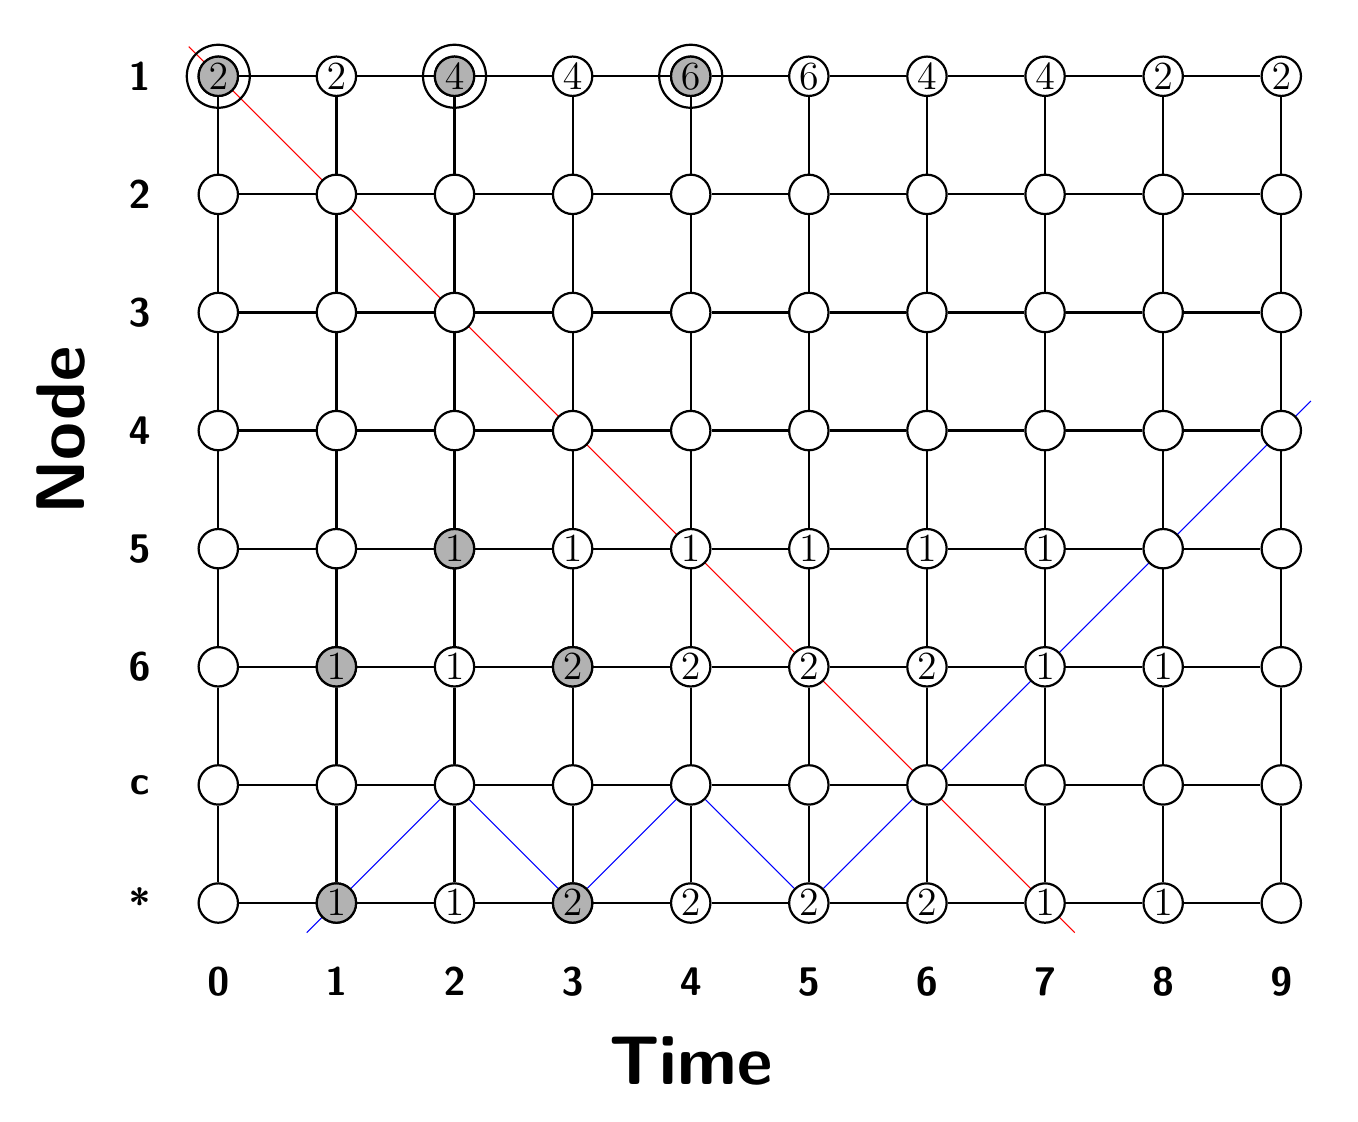
\begin{tikzpicture}[-,auto,node distance=1cm,
                    thick,main node/.style={circle,fill=white,draw,font=\sffamily\Large\bfseries,minimum size=0.5cm}]
 \foreach \x in {0,...,9}
    \foreach \y in {0,...,7} 
       {\pgfmathtruncatemacro{\label}{\x - 5 *  \y +21}
       \node [main node]  (\x\y) at (1.5*\x,1.5*\y) {};} 

  \foreach \x in {0,...,8}
   \foreach \y in {0,...,6}
    \pgfmathtruncatemacro{\za}{\y+1}
    \pgfmathtruncatemacro{\zb}{\x+1}
      \draw (\x\y)--(\x\za) (\x\y)--(\zb\y) ;
      
   \foreach \x in {0,...,8}
    \pgfmathtruncatemacro{\zb}{\x+1}
      \draw (\x7) -- (\zb7);
      
   \foreach \y in {0,...,6}
     \pgfmathtruncatemacro{\za}{\y+1} 
        \draw (9\y) -- (9\za);
        
        
%Labeling to the sides
  \foreach \y in {2,...,7}
   \pgfmathtruncatemacro{\label}{8-\y}
   \node[font=\sffamily\Large\bfseries] (Label\y) [shift={(-1,0)}] at (0\y) {\label};       
   
   \node[font=\sffamily\Large\bfseries] (Label) [shift={(-1,0)}] at (01) {c};
   \node[font=\sffamily\Large\bfseries] (Label) [shift={(-1,0)}] at (00) {*};
   
   \node[font=\sffamily\Huge\bfseries] (Axis) [shift={(-2,0)},rotate=90] at (04) {Node};

   \foreach \x in {0,...,9}
    \node[font=\sffamily\Large\bfseries] (Timelabel\x) [shift={(0,-1)}] at (\x0) {\x};
    
   \node[font=\sffamily\Huge\bfseries] (Axis) [shift={(0,-2)}] at (40) {Time};
    
    
%Adding in top attacks        
   \node[main node,fill=gray!60] (07) at (07) {};    
   \node[circle,draw,minimum size=0.8cm] (Attack1) at (07) {};
   
   \node[main node,fill=gray!60] (27) at (27) {};    
   \node[circle,draw,minimum size=0.8cm] (Attack2) at (27) {};     
   
   \node[main node,fill=gray!60] (47) at (47) {};    
   \node[circle,draw,minimum size=0.8cm] (Attack3) at (47) {};
   
   %Attack numbers
    \node[font=\sffamily\Large\bfseries] (AttackNumber1)  at (07) {$2$};
    \node[font=\sffamily\Large\bfseries] (AttackNumber1)  at (17) {$2$}; 
    \node[font=\sffamily\Large\bfseries] (AttackNumber1)  at (27) {$4$}; 
    \node[font=\sffamily\Large\bfseries] (AttackNumber1)  at (37) {$4$}; 
    \node[font=\sffamily\Large\bfseries] (AttackNumber1)  at (47) {$6$}; 
    \node[font=\sffamily\Large\bfseries] (AttackNumber1)  at (57) {$6$}; 
    \node[font=\sffamily\Large\bfseries] (AttackNumber1)  at (67) {$4$}; 
    \node[font=\sffamily\Large\bfseries] (AttackNumber1)  at (77) {$4$}; 
    \node[font=\sffamily\Large\bfseries] (AttackNumber1)  at (87) {$2$}; 
    \node[font=\sffamily\Large\bfseries] (AttackNumber1)  at (97) {$2$}; 
          
   
%Adding in middle attacks
  \node[main node,fill=gray!60] (23) at (23) {};
  \node[main node,fill=gray!60] (12) at (12) {};
  \node[main node,fill=gray!60] (32) at (32) {};
     
    %Attack numbers
    \node[font=\sffamily\Large\bfseries] (AttackNumber1)  at (23) {$1$};
    \node[font=\sffamily\Large\bfseries] (AttackNumber1)  at (33) {$1$}; 
    \node[font=\sffamily\Large\bfseries] (AttackNumber1)  at (43) {$1$}; 
    \node[font=\sffamily\Large\bfseries] (AttackNumber1)  at (53) {$1$}; 
    \node[font=\sffamily\Large\bfseries] (AttackNumber1)  at (63) {$1$}; 
    \node[font=\sffamily\Large\bfseries] (AttackNumber1)  at (73) {$1$};
     
    \node[font=\sffamily\Large\bfseries] (AttackNumber1)  at (12) {$1$}; 
    \node[font=\sffamily\Large\bfseries] (AttackNumber1)  at (22) {$1$}; 
    \node[font=\sffamily\Large\bfseries] (AttackNumber1)  at (32) {$2$}; 
    \node[font=\sffamily\Large\bfseries] (AttackNumber1)  at (42) {$2$}; 
    \node[font=\sffamily\Large\bfseries] (AttackNumber1)  at (52) {$2$}; 
    \node[font=\sffamily\Large\bfseries] (AttackNumber1)  at (62) {$2$}; 
    \node[font=\sffamily\Large\bfseries] (AttackNumber1)  at (72) {$1$}; 
    \node[font=\sffamily\Large\bfseries] (AttackNumber1)  at (82) {$1$};   
%Adding bottom attacks

 \node[main node,fill=gray!60] (10) at (10) {};
 \node[main node,fill=gray!60] (30) at (30) {};
 
    %Attack numbers
    \node[font=\sffamily\Large\bfseries] (AttackNumber1)  at (10) {$1$}; 
    \node[font=\sffamily\Large\bfseries] (AttackNumber1)  at (20) {$1$}; 
    \node[font=\sffamily\Large\bfseries] (AttackNumber1)  at (30) {$2$}; 
    \node[font=\sffamily\Large\bfseries] (AttackNumber1)  at (40) {$2$}; 
    \node[font=\sffamily\Large\bfseries] (AttackNumber1)  at (50) {$2$}; 
    \node[font=\sffamily\Large\bfseries] (AttackNumber1)  at (60) {$2$}; 
    \node[font=\sffamily\Large\bfseries] (AttackNumber1)  at (70) {$1$}; 
    \node[font=\sffamily\Large\bfseries] (AttackNumber1)  at (80) {$1$};        
        
                 
%Some example lines drawn
\begin{scope}[on background layer]
\node (a)[shift={(-0.5,0.5)}] at (07) {};
\node (b)[shift={(0.5,-0.5)}] at (70) {};
\draw[color=red] (a) -- (b);

\node (c)[shift={(-0.5,-0.5)}] at (10) {};
\node (d)[shift={(0.5,0.5)}] at (94) {};
\draw[color=blue] (c) -- (21) (21) -- (30) (30)--(41) (41) -- (50) (50)--(d);

\end{scope}

                   
\end{tikzpicture}}
\end{center}
\caption{Grid solution of $m=6$ on $S_{7}^{5}$ with two example paths}
\label{Figure:Example of attack below bound}
\end{myfigure}

\begin{conjecture}[Elongated star graph solution for $2(n-1) \leq m < 2(k+1)$]
For $2(n-1) \leq m < 2k$ we conjecture that,
$$V=\frac{2m}{2(n+k)+m+2(n-1)}$$
by the patroller using the combinatorial improvement (extended for odd $m$) and the attacker doing different strategies depending on $m$.
\end{conjecture}

\subsubsection{Plan}
\textbf{Time Estimate:} 1 Month

\textbf{Plan:} The type of attacking strategy for a variety of $m$ has been conjectured, along with some cyclic property of $m$ and which attack strategy should be picked. We need to formally define the attacks, then formally prove the cyclic relationship between $m$ and which attack strategy should be used. Then formal proof of the attacker bound needs to be fine, however this links in with the plan of section \ref{Section:Proof completions} and an idea of how to bring these proofs together into a need idea needs to formed.

\subsection{Proof completions}
\label{Section:Proof completions}
The proof for the time-limited diametric attack(see appendix \ref{Appendix:Proof of time-limited diametric attack}) needs consolidating and the general logic which will be used in the other similar proofs(see appendix \ref{Appendix:Proof of time-delayed attack} and \ref{Appendix:Proof of type-delayed attack}).

\subsubsection{Plan}
\textbf{Time Estimate:} 1 Month

\textbf{Plan:} Need to develop a way to combine all the proofs under a uniform idea and/or possibly rewrite them as smaller lemmas which build to a theorem. Notational convention needs to be picked so that the proof looks and reads cleanly. Getting across the idea of the spacing in time is what stops the patroller getting any more potential attacks.

\subsection{Complete numerical experiments for an instantaneously moving patroller}
\label{Section:Complete Numerical experiments for an instantaneously moving patroller}
The current code can only deal with deterministic attack times, as it was initially developed for local-observations. To deal with distributions functions, we must rewrite the code and how it formats the attack.

It also will prompt us to look into using probabilistic cycles around the state space in the local-observation set-up to find $g$ instead of using value iteration, which currently has the issue of periodicity and not converging. This could be avoided by recoding the heuristics to look at probabilistic cycles around the state space under the policy for each look-ahead window.

\subsubsection{Plan}
\textbf{Time Estimate:} 1 Month

\textbf{Plan:} To rewrite code to deal with generic attack distributions, by using functions and integration tables. To alter code to use a path selection which works out the optimal long-run average cost for the heuristic policy at a certain look-ahead, by the use of cycles. Then run numerical experiments, with the same set up as in \citep{Lin2013} and compare the results to the optimum. We also want to check if the same issue is found when we use purely deterministic attack times and whether splitting the index seems to help (as it does with local observations).

\subsection{Extending discrete attack time to generic distributions for local observations}
We want to look at removing the restriction placed on the attack time to be deterministic, as in section \ref{Section:Deterministic attack time assumption}. This will allow us to deal with any generic distribution, to do so we will focus on the single node problem with a generic distribution.

As before if we start in states $(B+1,v)$ we will renew if $g \leq c \lambda$ and by the neglecting strategy we know this is guaranteed. So the optimal strategy will have all states with $s=B+1$ renew immediately.

Now we will work backwards, aiming to use backwards recursion to work through to some multi-stage threshold policy, $\pi^{\text{TH}}(\bm{v}_{\text{crit}})$ where $(\bm{v}_{\text{crit}})_{i}$ is the threshold on the state space row of $s=i$. We expect this threshold to be triangular on the state space, that is that $\bm{v}_{\text{crit}}$ is a non-increasing vector.

\begin{definition}[Multi-stage threshold policy]
A policy, $\pi_{\text{Th}}(\bm{v}_{\text{crit}})$, is said to be a \textit{multi-stage threshold} policy, with thresholds, $\bm{v}_{\text{crit}}=(v_{\text{crit},1},...,v_{\text{crit},B+1}) \in \mathbb{Z}_{+}^{B+1}$, if in states $(s,v)$ we renew now if $v \geq v_{\text{crit},s}$ and otherwise we wait for one time period and then make the decision again.
\end{definition}

\begin{myfigure}
\begin{center}
\resizebox{0.9\linewidth}{!}{
\begin{tikzpicture}[-,auto,node distance=1cm,
                    thick,main node/.style={circle,fill=white,draw,font=\sffamily\large,minimum size=0.5cm}]
 \foreach \x in {0,...,5}
    \foreach \y in {0,...,4} 
       {\pgfmathtruncatemacro{\label}{\x - 5 *  \y +21}
        \pgfmathtruncatemacro{\v}{\x}
        \pgfmathtruncatemacro{\s}{5-\y}
       \node [main node]  (\x\y) at (1.5*\x,1.5*\y) {\s,\v};}
       
       \node[main node] (Renewal) at (1.5*6,1.5*4) {$\theta$};

 \foreach \x in {0,...,1}
    \foreach \y in {2,...,5} 
       {\pgfmathtruncatemacro{\label}{\x - 5 *  \y +21}
        \pgfmathtruncatemacro{\v}{\x}
        \pgfmathtruncatemacro{\s}{5-\y}
        \pgfmathtruncatemacro{\nv}{\v}
        \pgfmathtruncatemacro{\ns}{5-\y+1}
       \draw[->] (\nv\ns)--(\v\s);}
       
  \foreach \x in {2,...,5}
    \foreach \y in {2,...,2} 
       {\pgfmathtruncatemacro{\label}{\x - 5 *  \y +21}
        \pgfmathtruncatemacro{\v}{\x}
        \pgfmathtruncatemacro{\s}{5-\y}
        \pgfmathtruncatemacro{\nv}{\v}
        \pgfmathtruncatemacro{\ns}{5-\y+1}
       \draw[->] (\nv\ns)--(\v\s);}
       
    \foreach \x in {2,...,3}
    \foreach \y in {3,...,3} 
       {\pgfmathtruncatemacro{\label}{\x - 5 *  \y +21}
        \pgfmathtruncatemacro{\v}{\x}
        \pgfmathtruncatemacro{\s}{5-\y}
        \pgfmathtruncatemacro{\nv}{\v}
        \pgfmathtruncatemacro{\ns}{5-\y+1}
       \draw[->] (\nv\ns)--(\v\s);}

    \foreach \x in {4,...,5}
       {\draw[-] (\x3) to (1.5*\x,1.5 *2.4);}
                 
        \draw[-] (1.5*4,1.5*2.4) to (1.5*6,1.5*2.4);


    \foreach \x in {2,...,5}
       {\draw[-] (\x2) to (1.5*\x,1.5 *1.4);}
                 
        \draw[-] (1.5*2,1.5*1.4) to (1.5*6,1.5*1.4);
       
    \foreach \x in {2,...,5}
       {\draw[-] (\x1) to (1.5*\x,1.5 *0.4);}
                 
        \draw[-] (1.5*2,1.5*0.4) to (1.5*6,1.5*0.4);
        \draw[->] (1.5*6,1.5*0.4) to (Renewal);                          

    \foreach \x in {0,...,5}
       {\draw[-] (\x0) to (1.5*\x,-1.5*0.6);}
       
       \draw[-] (1.5*0,-1.5*0.6) to (1.5*6,-1.5*0.6);                                            
       \draw[-] (1.5*6,-1.5*0.6) to (1.5*6,1.5*0.4);                                 
       
    \foreach \x in {0,...,5}
    { 
     \draw[->,bend right,dashed] (Renewal) to (\x4);    
    }   
        

\node (XaxisLeft) [shift={(-0.5,0.5)}] at (05) {};
\node (XaxisRight) [shift={(1,0.5)}] at (55) {};

\node (YaxisBottom) [shift={(-1,-0.5)}] at (00) {};
\node (YaxisTop) [shift={(-1,1)}] at (05) {};

\draw[->,line width=1mm] (XaxisLeft)--(XaxisRight);
\draw[->,line width=1mm] (YaxisTop)--(YaxisBottom);

\node[font=\sffamily\large] (OLabel) [shift={(0.5,1)}] at (25) {Observation, $v_{j}$};
\node[font=\sffamily\large] (SLabel) [shift={(-1.5,0.5)}] at (02) {\rotatebox{90}{Time since last visit, $s_{j}$}};

\node[main node] (Example) [shift={(-1,0.5)}] at (05) {$(s_{j},v_{j})$};
   

\end{tikzpicture}
}
\end{center}
\caption{Threshold policy, $\pi_{\text{Th}}(6,4,2,2,0)$, with \textcolor{blue}{$b_{j}=5$} and \textcolor{red}{$B_{j}=4$} (e.g. $X_{j} \leq 3.7$)}
\end{myfigure}

As an example we will now start to work out what to  do in states $s=B$ and how to work out the threshold. We can do the same process in these states, either choosing to wait $0$ or $1$ time period and then renew, which are the policies $\pi^{\text{R}}$ and $\pi^{\text{NR}}$ respectively. Then,

\begin{align*}
&V_{n}^{\pi_{\text{R}}}(s,v)= \omega + E[V_{n-1}^{\sigma}(\theta)], \\
&V_{n}^{\pi_{\text{NR}}}(s,v)= c (vP(B-1 < X \leq B) + \lambda \int_{B-1}^{B} P(X \leq t ) dt) \omega + E[V_{n-1}^{\sigma}(\theta)]. \\
\end{align*}

With the policy $\pi^{\text{R}}$ being picked over $\pi^{\text{NR}}$ (or be indifferent) if

\begin{align*}
&\lim\limits_{n \rightarrow \infty} V_{n}^{\pi_{NR}} (B,v) - V_{n}^{\pi_{R}}(B,v) \geq 0 \\
& \iff \lim\limits_{n \rightarrow \infty} c (\lambda \int_{B-1}^{B} P(X \leq t ) dt + v P(B-1 < X \leq B)) + E[V_{n-1}^{\sigma}(B+1,0)] - (\omega + E[V_{n-1}^{\sigma}(\theta)]) \geq 0 \\
& \iff g \leq c (\lambda \int_{B-1}^{B} P(X \leq t ) dt +v P(B-1 < X \leq B)) = c( \lambda R_{B} + v p_{B})
\end{align*}
Where $R_{x} \equiv \int_{x-1}^{x} P(X \leq t ) dt = \int_{x-1}^{x} F(t) dt$ and $p_{x} \equiv P(x-1 < X \leq x) = F(x)-F(x-1)$ (For our generic distributions c.d.f $F$).

This means the bound for renewing now is almost the same as before, $g \leq c (\lambda R_{B} + v p_{B}) \equiv g_{B}$.

Now to decide if in $(B-1,v)$ we should renew or not we need to consider waiting zero,one or two periods before renewing (renew in $s=B-1,B,B+1$).

We could split ourself into cases, of $v$ such that $g \leq g_{B}$ (so if we wait we renew in $s=B$) or otherwise if we wait, we wait again and renew in $s=B+1$.

\subsubsection{Plan}
\textbf{Time Estimate:} 3 Months

\textbf{Plan:} To complete the backwards recursion case by case, to get the optimal policy to be that of a multi-stage threshold policy. Then to develop an index using the fair price for renewal in each state to allow us to form an index. Implement the index for numerical studies with some simple distributions e.g. uniform and triangular. We also want to investigate whether on two nodes that the IH performs optimally. We want to extend the theory further to have attackers wait until the patroller leaves before beginning their attack. 

\subsection{Strategic Patroller with Random Attackers on Edges}
We want to look at considering similar work to that in section, \ref{Section:Review of patrolling problem with random attackers} but instead of attackers arriving at nodes, we could consider attackers arriving on edges. We provide a brief introduction to this idea now focusing on directed graphs.

We use a directed graph, $Q=(N,E)$, with nodes $N=\{1,...,n \}$ and edges $E= \subset E_{\text{Comp}}= \{(i,j) \, | (i,j) \in N  \}$. We have our adjacency matrix, $A$, where $A_{i,j}$ means that a transition from node $i$ to node $j$ is possible.

Attackers arrive at each edge according to a Poisson process of rate, $\lambda_{i,j}$ and pick a position along the unit length edge according to a distribution function, $f_{i,j}(x)$ (with support, $x \in [0,1]$, and c.d.f, $F_{i,j}(x)$). The attack lasts, $X_{i,j}$ time units before completion and a cost is incurred to the patroller of $c_{i,j}$.

The patroller's strategy is a walk (with possible waiting at nodes), we will assume as before that they walk along the edges at unit speed, taking one time period to traverse one edge. The decisions are which edge to traverse next (which is equivalent to which node to walk to).

Our state space is $\Omega= \{ \bm{s}=(s_{i,j})_{(i,j) \in E} \, | \, s_{i,j}=1,2,... \; \forall (i,j) \in E \}$, where $s_{i,j}$ is the number of time periods since the edge $(i,j)$ was last traversed.

From a state, $\bm{s}$, we can identify the current node by $l(\bm{s}) = (\argmin_{(i,j)} \bm{s})_{2} $ the patroller can choose to move to $\mathcal{A}(\bm{s})= \{ j' \, | (A)_{l(\bm{s}),j'}=1 \}$  and choosing node, $j'$,is equivalent to choosing to traverse edge $(j,j')$. When node, $j'$ is chosen to be moved to we transition to state, $\phi(\bm{s},j')=\widetilde{\bm{s}}$ where $s_{l(\bm{s}),j}=1$ and $s_{i,j}=s_{i,j}+1 \; \forall (i,j) \in E \setminus \{(l(\bm{s}),j') \}$. 

Again the future of the process is independent of its past, we can formulate its  movement as a MC and the patroller's problem is a MDP.

The patroller incurs a cost at each edge for the next time period I.e $C(\bm{s},j')=\sum\limits_{(i,j) \in E} C_{i,j}(\bm{s},j')$ where $C_{i,j}(\bm{s},j')$ is the cost at the edge $(i,j)$ choosing to move to node $j'$ in the next time period. Hence

\begin{align*}
C_{i,j}(\bm{s})&= c_{i,j} \lambda_{i,j} \int_{0}^{1} f_{i,j}(y) \int_{0}^{s_{i,j}} P(t-1 < X_{i,j} \leq t) dt dy \\
&= c_{i,j} \lambda_{i,j} \int_{0}^{s_{i,j}} P(t-1 < X_{i,j} \leq t) dt \\
\end{align*}

\begin{note}
We note due to all edges being traversed at the same speed, the last time a point $x$ (from node $i$) along the edge $(i,j)$ was seen was $s_{i,j}-x$, so when it returned to it is seen in $x$ time, so is seen again in $s_{i,j}$ time.
\end{note}

As before we bound the attack times by, using $B_{i,j} \equiv \min \{ k \, | k \in \mathbb{Z}^{+} P(X_{i,j} \leq k)=1 \}$ to create a finite state space, $\Omega= \{\bm{s} \, | s_{i,j}=1,2,...,B_{i,j} \; \forall (i,j) \in E \}$ and our transition is modified to $\widetilde{s}_{i,j}=\min\{s_{i,j}+1,B_{i,j}+1 \} \; \forall (i,j) \in E \setminus \{(l(\bm{s}),j') \}$.

The objective again is to minimize the long-run average cost among all edges, and as we have a finite state space as before, we can focus on the class of stationary, deterministic policies, $\Pi = \{ \pi: \Omega \rightarrow E \, | \pi(\bm{s}) \in  \{(l(\bm{s}),j') \, | \, j \in \mathcal{A}(\bm{s}) \} \}$. We wish to solve,

\begin{align*}
C^{\text{OPT}}(\bm{s}_{0}) \equiv \min\limits_{\pi \in \Pi} \sum\limits_{(i,j) \in E} V_{i,j}(\pi,\bm{s}_{0})
\end{align*}
Where $V_{i,j}(\pi,\bm{s}_{0})$ is the long-run average cost incurred at edge $(i,j)$ under the policy, $\pi$, starting from state, $\bm{s}_{0}$, defined by,
\begin{align*}
V_{i,j}(\pi,\bm{s}_{0}) \equiv \lim\limits_{N \rightarrow \infty} \frac{1}{N} \sum\limits_{(i,j) \in E} C_{i,j}(\phi^{k}_{\pi}(\bm{s}_{0}),\pi(\phi^{k}_{\pi}(\bm{s}_{0})))
\end{align*}
Where $\phi^{k}_{\pi}(\bm{s}_{0})$ is the state after $k$ transitions starting from $\bm{s}_{0}$ under the policy $\pi$.


We now notice an extreme similarity to the `solved' problem in \ref{Section:Review of patrolling problem with random attackers} and in fact we can see a link between the edges here and the nodes in the original problem in \cite{Lin2013}. We seek some correspondence between the two problems by using the edge-vertex dual for directed graphs (see appendix \ref{Appendix:Graph Definitions} for a definition). This correspondence, allows us to use the heuristics and theory as section \ref{Section:Review of patrolling problem with random attackers}.

\begin{note}
The resultant edge-vertex dual graph is directed, but the original problem has no issue with this as it just a reduction in the action space for certain states.
\end{note}

If we are to consider undirected graphs, we shall point out that the cost function changes depending on which way we traverse the edge, due to how arrivals orientate themselves according to the distribution along the edges. We aim to solve such programs by expanding the state space, to consider which way the edge was last traversed and not just when.

\subsubsection{Plan}
\textbf{Time Estimate:} 2 Months

\textbf{Plan:} To extend the theory to deal with the undirected graph, which  will include modifying the cost function and state space for the opposite traversal of an edge. Then to isolate particular examples which can be `solved' with the previous reduction tools; such as acyclic graphs, which remove the dependency on which way the edges are traversed. The study of the class of  acyclic graphs will be important as all walks which consider using the same edge always traverse them in the opposite direction to as before. Then to see if there is a way to convert an undirected problem to a directed problem and hence use the correspondence for the solution. Finally we wish to try to solve it from first principals without any intuitive understanding.


\subsection{Investigate weighted graphs}
A weighted graph is a graph in which each edge has an associated number called its `weight', they are often used to represent distance. We suggest now using a weighted graph with the distance between locations in a graph.

That is a \textit{weighted graph}, $G=(N,E,w)$ where $w: E \rightarrow \mathbb{R}^{+}$ is a \textit{weight function} which assigns each edge to a real positive weight. As the patrol problem is currently an integer time problem we will assume that $w: E \rightarrow \mathbb{Z}^{+}$.

We propose that we can convert a weighted graph patrol problem for random attackers into a standard patrol problem for random attackers, by the directed sub-division of an integer weighted edge. This division introduces intermediate nodes which we will say that no waiting is possible, by changing the possible actions and we will have no attackers arrive at this node, by picking the probability to be zero. An example of how to convert the game can be seen in figure \ref{Figure:Example of converting a weighted patrol problem}.

\begin{note} 
we note that waiting is not allowed at intermediate nodes and we have directed edges, so the adjacency matrix will not be symmetric. However we conjecture that this has no affect on the theory and heuristic.
\end{note}

\begin{myfigure}
\begin{center}
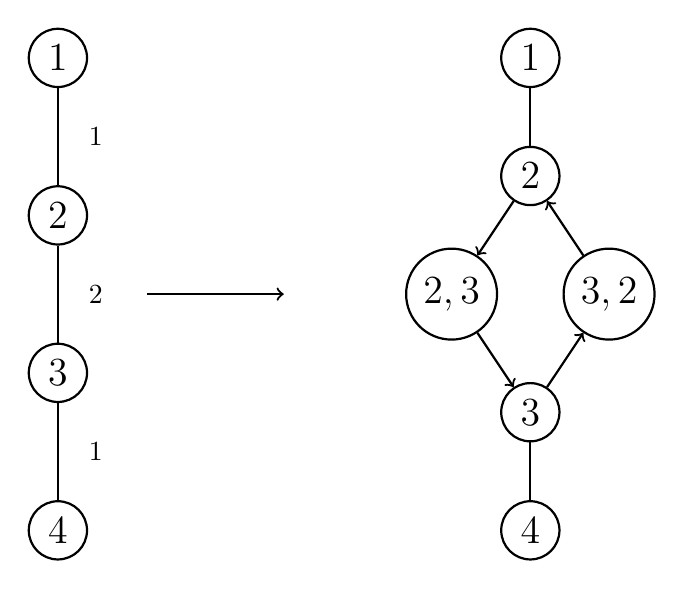
\begin{tikzpicture}[baseline=(current bounding box.north),-,auto,node distance=2cm,
                    thick,main node/.style={circle,draw,font=\sffamily\Large\bfseries}]

  \node[main node] (1) {$1$};
  \node[main node] (2) [below of=1] {$2$};
  \node[main node] (3) [below of=2] {$3$};
  \node[main node] (4) [below of=3] {$4$};

  \node (P1) [shift={(1,-1)}] at (2) {};
  \node (P2) [right of=P1] {};
  
  \draw[->] (P1) edge (P2);
  
  \node[main node] (a1) [shift={(3,3)}] at (P2) {$1$};
  \node[main node] (a2) [shift={(3,1.5)}] at (P2) {$2$};
  \node[main node] (a3) [right of=P2] {$2,3$};
  \node[main node] (a4) [right of=a3] {$3,2$};
  \node[main node] (a5) [shift={(3,-1.5)}] at (P2) {$3$};
  \node[main node] (a6) [shift={(3,-3)}] at (P2) {$4$};

  \draw  (1)--(2) node[pos=0.5,label=right:$1$] {};
  \draw  (2)--(3) node[pos=0.5,label=right:$2$] {};
  \draw  (3)--(4) node[pos=0.5,label=right:$1$] {};
  
  \draw (a1) --(a2);
  \draw[->] (a2) to (a3);
  \draw[->] (a3) to (a5); 
  \draw[->] (a5) to (a4);
  \draw[->] (a4) to (a2);
  \draw (a5)--(a6);   
  
     
\end{tikzpicture}
\end{center}
\caption{Converting a weighted edge.}
\label{Figure:Example of converting a weighted patrol problem}
\end{myfigure}

We could then use a similar theory as in section 4 of \cite{Lin2013} to get heuristics for both a strategic attacker and patroller, to find near optimal answers for a the weighted version of the patrolling game. We also want consider alternative approaches to solve the weighted patrol problem, as for large weights this approach is suggested to become intractable. Consider the example as in figure \ref{Figure:Example of converting a weighted patrol problem} but with $(2,3)$ having a weight of $1000$ , then $2000$ nodes are introduced to convert the problem.

This may bring up an issue with how the proposed heuristics in \cite{Lin2013} look into the future, as they will be unable to see the actual nodes and therefore the indices, we propose that it is possible to `ignore' these nodes with such low indices.

We may also want to consider non-integer weights for a weighted patrol problem, then for rational weights it is a case of scaling. For irrational weights rounding and scaling is proposed. However we believe it is possible a more elegant way to think about the problem exists. 


\subsubsection{Plan}
\textbf{Time Estimate:} 2 Months

\textbf{Plan:} We first need to show that for a graph with an asymmetric adjacency matrix that the theory in \ref{Section:Review of patrolling problem with random attackers} still holds (which it will as only the Action set changes). We will then check that the heuristic still works optimally and that having an asymmetric matrix does not affect it that much. We then need to formalize the conversion between the weighted patrol problem with random attackers and the standard patrol problem with random attackers. After this we need to look at how we can use the heuristic depth when nodes which are far apart are the only ones with indices, by possibly altering the heuristic to `ignore' nodes of insignificant index and performing numerical experiments.

\subsection{Investigate types of patrolling}
Further to the idea that the patroller may overlook an attacker (\cite{Lin2014}), we may propose that not only can the patroller make the decision of where to move to, but also in what `mode' they search the region, fast or slow, each with different chances of overlook.

We believe that in the single-node problem version, we can introduce two service costs; a slow cost, $\omega_{s}$; and a fast cost, $\omega_{f}$ with long run service rates; a slow service rate, $\mu_{s}$; and a fast service rate, $\mu_{f}$ .We expect to get similar results to those in theorem 2 in \cite{Lin2014}, that is that for fixed service rates, $\mu_{s},\mu_{f}$ we expect to visit the node in mode, slow every $\frac{1}{\mu_{s}}$ time units, and fast every $\frac{1}{\mu_{f}}$.

However we may run into the issue in which we wish to visit every $4$ in slow and every $3$ in fast, then every $12$ we wish visit in both slow and fast simultaneously. We may propose an even more relaxed game in which the patroller can visit the single node in multiples modes upon each visit. When developing an index heuristic, we will assign an index to nodes which is the sum of two mode indices for the node(form the slow and fast game separation), then deciding the mode by which mode index provided a greater value to the sum.

\subsubsection{Plan}
\textbf{Time Estimate:} 3 Months

\textbf{Plan:} Reread \cite{Lin2014} and try to rewrite the Lagrangian relaxation to relax to two separate single node games. Use the theory in section 3.2/3.3 in \cite{Lin2014} for the two separate(slow/fast) games to have two indices for the two modes. We need to look the technical side of the theory to see if we can sum the indices for the combined game, making it a staged decision of when to visit and then in which mode. Once the technical details are checked we need to provide numerical experiments to see how good these heuristics are. We can then look at moving this into a strategic game for the attacker using the same idea as in section 4 of \cite{Lin2014}(or equally section 4 in \cite{Lin2013}).


%End of main part of document
\bibliography{mybib}

\newpage
\appendix
\pagenumbering{roman}
\appendixpage
\addappheadtotoc
\section{Graph Definitions}
\label{Appendix:Graph Definitions}
\begin{definition}[Graph]
A \textit{graph}, $G=G(N,E)$, is made up of: a set of \textit{nodes} (also called \textit{vertices} or \textit{points}), $N$, which are places ; and a set of \textit{edges} (also called \textit{arcs} or lines), $E$, which are connections between places, so elements of $E$ must be two-element subsets of $N$.
\end{definition}

\begin{note}
For notational purposes both $e_{i,i'} \in E$ and $(i,i') \in E$ are equivalent.
\end{note}

\begin{definition}[Adjacency,Incidency]
We say nodes, $n,m$ are \textit{adjacent} if $\exists (n,m) \in E$ and we say the edge $(n,m)$ is \textit{incident} to both $n$ and $m$.
\end{definition}

\begin{definition}[Adjacency matrix]
A graph, $G$, can be reprsented as an \textit{adjacency matrix}, $A$, where $A_{i,j}=1 \iff (i,j) \in E$
\end{definition}

\begin{definition}[Subgraph]
A graph $Q'=(N',E')$ is said to be a \textit{subgraph} of $Q=(N,E)$ if $N' \subset N$ and $E' \subset E$.

A subgraph is said to be \textit{induced} by $N'$ (or \textit{edge-preserving}) if $E'$ contains all edges (from $E$) that have both end points in $N'$.
\end{definition}


\begin{myfigure}
\begin{center}
\begin{submyfigure}{.3\textwidth}
\begin{center}
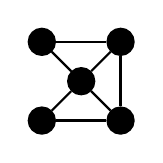
\begin{tikzpicture}[baseline=(current bounding box.north),-,auto,node distance=1cm,
                    thick,main node/.style={circle,draw,fill,font=\sffamily\bfseries}]

  \node[main node] (1) {};
  \node[main node] (2) [right of=1] {};
  \node[main node] (3) [shift={(0.5,-0.5)}] at (1) {};
  \node[main node] (4) [below of=1] {};
  \node[main node] (5) [below of=2] {};
  

  \path[every node/.style={font=\sffamily}]
    (1) edge  (2)
        edge  (3)
    (2) edge  (3)
        edge  (5)
    (4) edge  (3)
        edge  (5)
    (5) edge  (3);
                        
\end{tikzpicture}
\end{center}
\caption{$Q$}
\label{subexamplefigure: before subgraphs}
\end{submyfigure}
\begin{submyfigure}{.3\textwidth}
\begin{center}
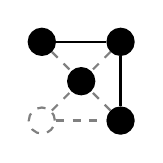
\begin{tikzpicture}[baseline=(current bounding box.north),-,auto,node distance=1cm,
                    thick,main node/.style={circle,draw,fill,font=\sffamily\bfseries}, alt node/.style={circle,draw,dashed,gray,font=\sffamily\bfseries}]

  \node[main node] (1) {};
  \node[main node] (2) [right of=1] {};
  \node[main node] (3) [shift={(0.5,-0.5)}] at (1) {};
  \node[alt node] (4) [below of=1] {};
  \node[main node] (5) [below of=2] {};
  

  \path[every node/.style={font=\sffamily}]
    (1) edge  (2)
    (2) edge  (5);
    
  \path[dashed,gray,font=\sffamily]
    (1) edge (3)
    (2) edge (3)
    (4) edge (3)
        edge (5)
    (5) edge (3);          
                        
\end{tikzpicture}
\end{center}
\caption{$Q_{1}$}
\label{subexamplefigure: subgraph}
\end{submyfigure}
\begin{submyfigure}{.3\textwidth}
\begin{center}
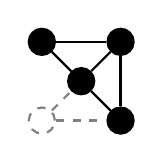
\begin{tikzpicture}[baseline=(current bounding box.north),-,auto,node distance=1cm,
                    thick,main node/.style={circle,draw,fill,font=\sffamily\bfseries}, alt node/.style={circle,draw,dashed,gray,font=\sffamily\bfseries}]

  \node[main node] (1) {};
  \node[main node] (2) [right of=1] {};
  \node[main node] (3) [shift={(0.5,-0.5)}] at (1) {};
  \node[alt node] (4) [below of=1] {};
  \node[main node] (5) [below of=2] {};
  

  \path[every node/.style={font=\sffamily}]
    (1) edge  (2)
    (2) edge  (5)
    (1) edge (3)
    (2) edge (3)
    (5) edge (3);
    
  \path[dashed,gray,font=\sffamily]
    (4) edge (3)
        edge (5);          
                        
\end{tikzpicture}
\end{center}
\caption{$Q_{1}$}
\label{subexamplefigure: induced subgraph}
\end{submyfigure}
\caption{ $Q_{1}$ is a subgraph of $Q$. However it is not induced as it is missing possible edges connecting nodes that existed in $Q$. $Q_{2}$ shows the induced subgraph on the chosen set of nodes. }
\end{center}
\label{examplefigure: subgraph example}
\end{myfigure}

\begin{definition}[Edge-preserving subgraph]
A subgraph, $Q'=(N',E')$ of $Q$ is called edge-preserving if $n_{1},n_{2} \in Q \cap Q*$ then if $(n_{1},n_{2}) \in E \implies (n_{1},n_{2}) \in E'$ 
\end{definition}

\begin{definition}[Edge types]
An edge $(i,i)$ is called a \textit{loop}. If more than one copy of the edge $(i,j)$ exits in $E$, it is said to be a \textit{multiple edge}. A \textit{simple graph} is graph without any loops or multiple edges.
\end{definition}

\begin{definition}[Node Identification]
The operation of \textit{node identification} on two nodes, $u$ and $v$, of a graph, $G=(N,E)$ into a single node $w$, is a mapping $f:N \rightarrow N'$ resulting in a new graph $G'=(N',E')$ where $N'=(N \setminus  \{u,v\}) \cup \{w\}$ with $E'=E \setminus \{(u,v)\}$ if $(u,v) \in E$ and under the condition that $\forall x \in N$, $f(x) \in N'$ is incident to $e' \in E'$ iff $e \in E$ is incident to $x \in N$.
Furthermore if a graph, $Q$, undergoes repeated node identification to become $Q'$ then we say it has been \textit{simplified}. 
\end{definition}

\begin{definition}[Embedding]
An \textit{embedding} of a graph, $G$, onto a surface(compact, connected 2-manifold), $\Sigma$, is a representation of $G$ in $\Sigma$ in which points are associated with nodes and simple arcs(homeomorphic images of $[0,1]$) are associated with edges such that
\begin{itemize}
\item the end points of arc are the points associated with the nodes indecent with the edge
\item no arcs include points associated with other nodes
\item two arcs never intersect at a point which is interior to either of the arcs
\end{itemize}
\end{definition}

\begin{definition}[Planar]
A graph, $G$, is called \textit{planar} if it can be embedded in the plan $\mathbb{R}^{2}$.
\end{definition}

\begin{definition}[Distance,diameter]
The \textit{distance} between node $i$ and node$i'$ is the minimum number of edges between $i$ and $i'$ denoted, $d(i,i')$.
A graph's \textit{diameter} is the maximum distance between any pair of nodes, defined by $\bar{d} \equiv \max\limits_{i,i' \in N} d(i,i')$. Any pair of nodes $i$,$i'$ that are the diameter apart(i.e $d(i,i')=\bar{d}$) are called \textit{diametrical} 
\end{definition}

\begin{definition}[Walk,Path,Trail,Cycle]
A sequence of nodes $(n_{0},n_{1},...,n_{l})$ is a \textit{walk} of length $l$ if $e_{n_{i},n_{i+1}} \in E$ $\forall i=0,...,l-1$. Corresponding to a walk is the sequnece of $l$ edges $(e_{n_{0},n_{1}},e_{n_{1},n_{2}},...,e_{n_{l-1},n_{l}})$.

A walk becomes a trail if each edge in the walk is distinct, i.e $e_{n_{i},n_{i+1}} \neq e_{n_{j},n_{j+1}} \forall i \neq j$. A trail becomes a path if each node in the walk is distinct (except possibly the start and final node), i.e $n_{i} \neq n_{j} \forall i \forall i < j \geq l-1$.

A walk,trail or path is said to be \textit{closed} if the start and end nodes are the same. A \textit{cycle} is a closed path with length, $l \geq 3$ (with the special case of $l=3$ being called a \textit{triangle}).
\end{definition}

\begin{definition}[Hamiltonian cycle]
A \textit{Hamiltonian cycle} is a cycle which contains every node on the graph, i.e it is a cycle of length $l=|N|$. A graph that exhibits a Hamiltonian cycle is called \textit{Hamiltonian}
\end{definition}

\begin{figure}
\begin{center}
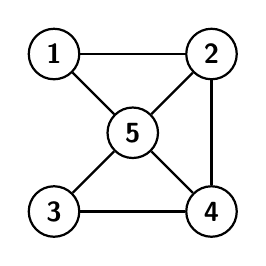
\begin{tikzpicture}[baseline=(current bounding box.north),-,auto,node distance=2cm,
                    thick,main node/.style={circle,draw,font=\sffamily\bfseries}]

  \node[main node] (1) {1};
  \node[main node] (2) [right of=1] {2};
  \node[main node] (3) [shift={(1,-1)}] at (1) {5};
  \node[main node] (4) [below of=1] {3};
  \node[main node] (5) [below of=2] {4};
  

  \path[every node/.style={font=\sffamily}]
    (1) edge  (2)
        edge  (3)
    (2) edge  (3)
        edge  (5)
    (4) edge  (3)
        edge  (5)
    (5) edge  (3);
                        
\end{tikzpicture}
\end{center}
\caption{Graph, $Q$}
\label{figure: walks on graph Q}
\end{figure}

\begin{example}
For the graph $Q$ as in Figure \ref{figure: walks on graph Q}:
\begin{itemize}
\item An example of a walk is $(1,2,1,5,4,2)$
\item An example of a trail is $(1,2,5,3,4,5,1)$
\item An example of a path is $(1,2,4,3)$
\item An example of a Hamiltonian cycle is $(1,2,4,3,5,1)$
\end{itemize}
Hence we would call the graph $Q$ Hamiltonian.
\end{example}

\begin{definition}[Complete graphs]
The \textit{complete graph}, $K_{n}$, is a graph of $n$ nodes, in which all edges are present, i.e $e_{i,i'} \in E \; \forall i,i' \in N$.
\end{definition}

\begin{myfigure}
\begin{center}
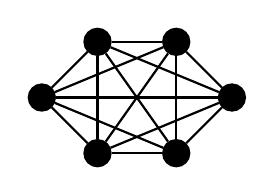
\begin{tikzpicture}[baseline=(current bounding box.north),-,auto,node distance=1cm,
                    thick,main node/.style={circle,fill,draw,font=\sffamily\bfseries}]

  \node[main node] (1) {};
  \node[main node] (2) [right of=1] {};
  \node[main node] (3) [below left of=1] {};
  \node[main node] (4) [below right of=2] {};
  \node[main node] (5) [below right of=3] {};
  \node[main node] (6) [below left of=4] {};
  

  \path[every node/.style={font=\sffamily}]
    (1) edge  (2)
        edge  (3)
        edge  (4)
        edge  (5)
        edge  (6)
    (2) 
        edge  (3)
        edge  (4)
        edge  (5)
        edge  (6)
    (3) 
        edge  (4)
        edge  (5)
        edge  (6)
    (4) edge  (5)
        edge  (6)
    (5) edge  (6);        
                     
\end{tikzpicture}
\caption{The complete graph of $6$ nodes,$K_{6}$.}
\end{center}
\end{myfigure}

\begin{definition}[Bipartite]
A graph is said to be \textit{bipartite} if $N=A \cup B$, where $A \cap B= \emptyset$ ,and $e_{i,i'} \notin E \, \forall i,i' \in A$, $e_{i,i'} \notin E \, \forall i,i' \in B$.
\end{definition}

\begin{definition}[Complete bipartite]
The \textit{complete biparite graph}, $K_{a,b}$, is a bipartite graph of $a+b$ nodes (where $|A|=a$,$|B|=b$), in which all edges are present, i.e $e_{i,i'} \in E \; \forall i \in A \, \forall i' \in B$ and $e_{i,i'} \in E \; \forall i \in B \, \forall i' \in A$.
\end{definition}

\begin{myfigure}
\begin{center}
\begin{submyfigure}{.45\textwidth}
\begin{center}
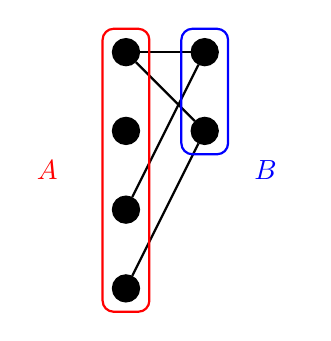
\begin{tikzpicture}[baseline=(current bounding box.north),-,auto,node distance=1cm,
                    thick,main node/.style={circle,draw,fill,font=\sffamily\bfseries}]

  \node[main node] (1) {};
  \node[main node] (2) [below of=1] {};
  \node[main node] (3) [below of=2] {};
  \node[main node] (4) [below of=3] {};
  \node[main node] (5) [right of=1] {};
  \node[main node] (6) [below of=5] {};
  

  \path[every node/.style={font=\sffamily}]
    (1) edge  (5)
        edge  (6)
    (3) edge  (5)
    (4) edge  (6);
        
  \node (ABox) [draw,rounded corners,red, fit= (1) (2) (3) (4)] {};
  \node (BBox) [draw,rounded corners,blue, fit= (5) (6)] {};
  
  \node [left=0.5cm,text width=0.5cm,red] at (ABox) {$A$};
  \node [right=1.5cm,text width=0.5cm,blue] at (ABox) {$B$};              
                     
\end{tikzpicture}
\end{center}
\caption{$Q$}
\label{subfigure: bipartite Q}
\end{submyfigure}
\begin{submyfigure}{.45\textwidth}
\begin{center}
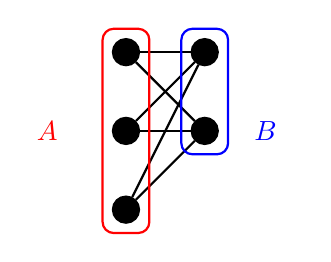
\begin{tikzpicture}[baseline=(current bounding box.north),-,auto,node distance=1cm,
                    thick,main node/.style={circle,draw,fill,font=\sffamily\bfseries}]

  \node[main node] (1) {};
  \node[main node] (2) [below of=1] {};
  \node[main node] (3) [below of=2] {};
  \node[main node] (4) [right of=1] {};
  \node[main node] (5) [below of=4] {};
  

  \path[every node/.style={font=\sffamily}]
    (1) edge  (4)
        edge  (5)
    (2) edge  (4)
        edge  (5)
    (3) edge  (4)
        edge  (5);
        
  \node (ABox) [draw,rounded corners,red, fit= (1) (2) (3)] {};
  \node (BBox) [draw,rounded corners,blue, fit= (4) (5)] {};
  
  \node [left=0.5cm,text width=0.5cm,red] at (ABox) {$A$};
  \node [right=1.5cm,text width=0.5cm,blue] at (ABox) {$B$};              
                     
\end{tikzpicture}
\end{center}
\caption{$K_{3,2}$}
\label{subfigure: complete bipartite}
\end{submyfigure}
\caption{ \ref{subfigure: bipartite Q} is an example of a bipartite graph, Q. \ref{subfigure: complete bipartite} is the complete bipartite graph with set sizes of $3$ and $2$.}
\end{center}
\end{myfigure}

\begin{definition}[Subdivision,Smoothing]
A \textit{Subdivision} (or \textit{expansion}) of a graph, $G$, is a new graph $G'$ which is made by subdividing a chosen edge. The subdivision of an edge $\{u,v\}$ yields a graph with a new node $w$ and the splitting of the edge $\{u,v\}$ into $\{u,w\}$ and $\{w,v\}$.

The reverse process is called \textit{Smoothing} of a graph, $G$, is a new graph $G'$ which is made by smoothing between two nodes. The smoothing out of a node pair $(u,v)$, with $d(u,v)=2$ and with $w$ between them, then $w$ is removed along with the edges $\{u,w\}$ and $\{v,w\}$, then the edge $\{u,v\}$ is placed to connect $u$ and $v$. 
\end{definition}

\begin{myfigure}
\begin{center}
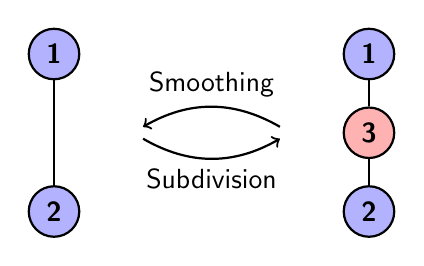
\begin{tikzpicture}[baseline=(current bounding box.north),-,auto,node distance=2cm,
                    thick,main node/.style={circle,draw,font=\sffamily\bfseries}]

  \node[main node,fill=blue!30] (1) {1};
  \node[main node,fill=blue!30] (2) [below of=1] {2};
  

  \path[every node/.style={font=\sffamily}]
    (1) edge  (2);
    
  \node (AP1) [shift={(1,-1)}] {};
  \node (AP2) [shift={(3,-1)}] {};
  
  \path[->,bend right,every node/.style={font=\sffamily}]
    (AP1) edge node[below] {Subdivision} (AP2)
    (AP2) edge node[above] {Smoothing} (AP1);
      
  
  \node[main node,fill=blue!30] (3) [shift={(4,0)}]{1};
  \node[main node,fill=red!30] (4) [shift={(4,-1)}]{3};
  \node[main node,fill=blue!30] (5) [shift={(4,-2)}]{2};
  
  \path[every node/.style={font=\sffamily}]
    (3) edge  (4)
    (4) edge  (5);
  
    
                        
\end{tikzpicture}
\caption{Subdivision and Smoothing of the edge $\{1,2\}$}
\end{center}
\end{myfigure}

\begin{definition}[Edge-vertex dual]
A \textit{edge-vertex dual} of a directed graph $G$, called $EV(G)$, is made of a vertex set $V_{EV(G)}=E_{G}$ and whose edge set is made up of a directed edge between $e_{1},e_{2} \in V_{EV(G)}$ if in $G$ the edge $e_{1}$'s head meets the tail of $e_{2}$ at some node.
\end{definition}

\begin{myfigure}
\begin{center}
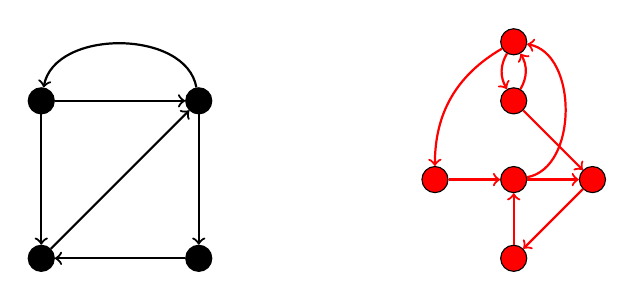
\begin{tikzpicture}[baseline=(current bounding box.north),-,auto,node distance=2cm,
                    main node/.style={circle,draw,fill=black,font=\sffamily\bfseries}]

  \node[main node] (1) {};
  \node[main node] (2) [right of=1] {};
  \node[main node] (3) [below of=1] {};
  \node[main node] (4) [below of=2] {};
  

  \path[thick,->]
  (1) edge (2);
  
  \path[thick,->,bend right=80]
  (2) edge (1);
  
  \path[thick,->]
  (2) edge (4)
  (4) edge (3)
  (1) edge (3)
  (3) edge (2);
  
  \node[main node,fill=red] (1a) [shift={(6,0)}] at (1) {};
  \node[main node,fill=red] (2a) [shift={(0,0.75)}] at (1a) {};
  \node[main node,fill=red] (3a) [shift={(1,-1)}] at (1a) {};
  \node[main node,fill=red] (4a) [shift={(0,-2)}] at (1a) {};
  \node[main node,fill=red] (5a) [shift={(-1,-1)}] at (1a) {};
  \node[main node,fill=red] (6a) [shift={(0,-1)}] at (1a) {};
  
  \path[thick,->,bend right=30,red]
  (1a) edge (2a);
  
   \path[thick,->,bend right=30,red]
  (2a) edge (1a)
  (2a) edge (5a);
  
   \path[thick,->,red]
   (1a) edge (3a)
   (3a) edge (4a)
   (4a) edge (6a)
   (5a) edge (6a)
   (6a) edge (3a);
   
   \path[thick,->,bend right=80,red]
   (6a) edge (2a); 
 
\end{tikzpicture}
\end{center}
\caption{A graph $G$ and its directed edge-vertex dual, $EV(G)$}
\end{myfigure}

\section{Examples}
\subsection{Example of decomposition}
\label{Appendix:Example of deocmposition}
\begin{example}
For $Q$ as seen in Figure \ref{Figure:Q decompisition example}. Consider when $m=3$, the decomposition of $Q$ into the graphs $Q_{1} \equiv L_{2}$ and $Q_{2} \equiv L_{3}$. $V_{1}=V(L_{2})=1$ as alternating between $1$ and $2$ can catch every attack. $V_{2}=V(L_{3})=\frac{3}{4}$ (as seen in \cite{Alpern2011}). 

Then we can get the bound $V \geq \frac{1}{\frac{1}{V_{1}}+\frac{1}{V_{2}}} = \frac{1}{\frac{1}{1}+\frac{3}{4}}=\frac{4}{7}$.
\end{example}

\begin{myfigure}
\begin{center}
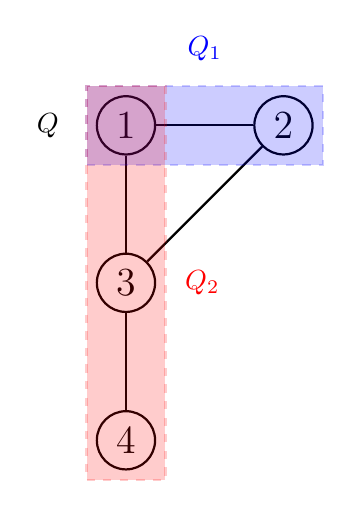
\begin{tikzpicture}[baseline=(current bounding box.north),-,auto,node distance=2cm,
                    thick,main node/.style={circle,draw,font=\sffamily\Large\bfseries}]

  \node[main node] (1) {$1$};
  \node[main node] (2) [right of=1] {$2$};
  \node[main node] (3) [below of=1] {$3$};
  \node[main node] (4) [below of=3] {$4$};

  \path[every node/.style={font=\sffamily}]
    (1) edge  (2)
    edge (3)
    (2) edge (3)
    (3) edge (4);
  
  \node (Box1) [draw=blue,dashed,thick,fit=(1) (2),fill=blue,opacity=0.2] {};  
  \node (Box2) [draw=red,dashed,thick,fit=(1) (3) (4),fill=red,opacity=0.2] {};
  
  \node [yshift=3.0ex, blue] at (Box1.north) {$Q_{1}$};
  \node [xshift=3.0ex, red] at (Box2.east) {$Q_{2}$};  
\node [left=0.5cm,text width=0.5cm] at (1)
{
$Q$
};   
\end{tikzpicture}
\end{center}
\caption{Decomposition of Q into \textcolor{blue}{$Q_{1}$} and \textcolor{red}{$Q_{2}$}.}
\label{Figure:Q decompisition example}
\end{myfigure}

\subsection{Example of simplification}
\label{Appendix:Example of simplification}
\begin{example}
For $Q$ as seen in Figure \ref{Figure:Q simplification example}, when $m=3$, the simplification of the graph by identifying nodes $1$ and $2$ simplifies $Q$ to $Q'=L_{3}$. Hence we can get the bound that $V(L_{3}) \geq  V(Q)$ so $V(Q) \leq \frac{3}{4} $
\end{example}

\begin{myfigure}
\begin{center}
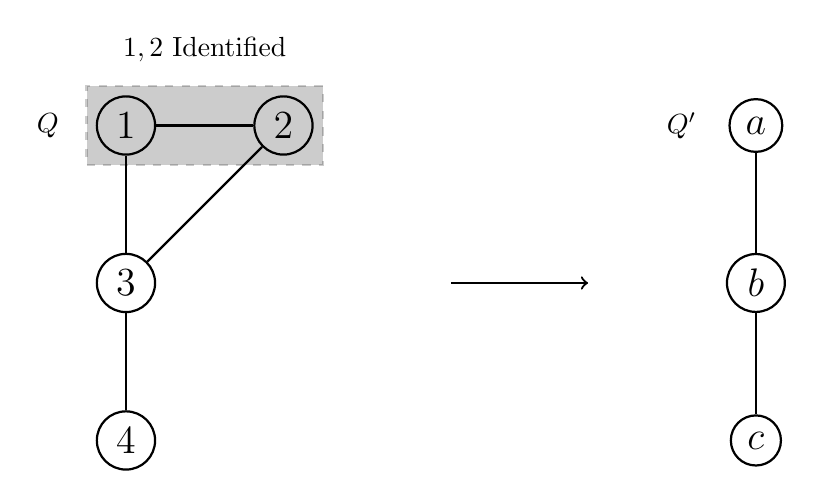
\begin{tikzpicture}[baseline=(current bounding box.north),-,auto,node distance=2cm,
                    thick,main node/.style={circle,draw,font=\sffamily\Large\bfseries}]

  \node[main node] (1) {$1$};
  \node[main node] (2) [right of=1] {$2$};
  \node[main node] (3) [below of=1] {$3$};
  \node[main node] (4) [below of=3] {$4$};
  
  \node (P1) [below of=2] {};
  \node (P2) [right of=P1] {};
  \node (P3) [right of=P2] {};
  
  \draw[->] (P2) edge (P3);
  
  \node[main node] (b) [right of=P3] {$b$};
  \node[main node] (a) [above of=b] {$a$};
  \node[main node] (c) [below of=b] {$c$};

  \path[every node/.style={font=\sffamily}]
    (1) edge  (2)
    edge (3)
    (2) edge (3)
    (3) edge (4)
    (a) edge (b)
    (b) edge (c);
  
  \node (Box1) [draw,dashed,thick,fit=(1) (2),fill,opacity=0.2] {};  
  
  \node [yshift=3.0ex] at (Box1.north) {$1,2$ Identified};  
\node [left=0.5cm,text width=0.5cm] at (1) {$Q$};
\node [left=0.5cm,text width=0.5cm] at (a) {$Q'$};   
\end{tikzpicture}
\end{center}
\caption{Simplifcation of $Q$ to $Q'$ by identification.}
\label{Figure:Q simplification example}
\end{myfigure}

\section{Patrolling games}
\subsection{Proof of diametric waiting time}
\label{Appendix:Proof of diametric waiting time}

Consider visit $i$ to a end node capturing $C_{i}$ of the attacks placed by the diametric attack, then the total number of attacks captured is $C=\sum\limits_{i=0}^{\floor{\frac{T-1}{\bar{d}}}} C_{i}$.

Then leaving the initial node at time $t$ gives us, $C_{0}=\min(t,T-m+1)$ , $C_{i}=\pospart{\min(t+i \bar{d},m,T-(t+i \bar{d})}$ for $i \neq 0$.

We first note that $C_{0}$ is increasing in the region $t \leq T-m$ and constant for $t \geq T-m+1$. So $C_{0}$ is concave. Due to this being increasing, and therefore its only possible to have others increasing if $t \leq T-m$, we will make this an assumption.

Now we look at $C_{i}$ and see it is increasing for the region $t \leq m-1-i\bar{d}$, constant for $m-i\bar{d} \leq t \leq T-1-m-i \bar{d}$ and decreasing for $ T-m-i \bar{d} \leq t \leq T-i \bar{d}-1$. So $C_{i}$ is concave. Hence $C$ is concave and so finding the best choice for $t$ is when the net increase is constant (or decreasing for the first time).

We see that $C_{0}$ always improves, contributing $1$ to the net increase. $C_{i}$ however is only increasing, and contributes $1$, if $i \leq \frac{m-1-t}{\bar{d}} < 2$ (as $m \leq 2\bar{d}$), so only $C_{1}$ can possibly contribute an increase when $t \leq m-\bar{d}-1$.

$C_{i}$ is decreasing, contributing $-1$ if $\frac{T-m-t}{\bar{d}} \leq i \leq \frac{T-1-t}{\bar{d}}$, with at most $2$ $C_{i}$'s being decreased (as the gap is $\frac{m}{2 \bar{d}}$ and $\bar{d} < m \leq 2 \bar{d}$).

This worst issue occurs when $\frac{T-m-t}{\bar{d}}$ or $\frac{T-1-t}{\bar{d}}$ are integers, meaning we have chosen $t=T-m-k\bar{d}$ or $t=T-1-k\bar{d}$ for some $k \in \mathbb{Z}$.

So overall increasing $t$ to $t+1$, with $t \leq m-\bar{d}-1$, gives us a net increase $1$ when we have non-integers, $0$ when we have integers  and $-1$ if $t > m- \bar{d}-1$.

So we pick the upper concave region, as its about to go from increasing to decreasing, giving us a choice of $t=m-\bar{d}$.
 
Note. $t=m-\bar{d}-1$ is not net decreasing, but $t=m-\bar{d}-1$ is net decreasing, so $t=m-\bar{d}$ is a choice for the maximum.

\subsection{Proof of conditions on T for diametric attack}
\label{Appendix:Proof of conditions on T for diametric attack}

We first justify the counting formula,

\begin{align*}
&\underbrace{m-\bar{d}}_{\text{Waiting initially}} + \underbrace{\pospart{m \times \left( M +1 \right)}}_{\text{Visits which get exactly } m \text{ attacks}} \\
&+ \underbrace{\pospart{T- \left( m-1 + \left(M +1 \right) \bar{d} \right)}+\pospart{T- \left( m-1 + \left(M +2 \right) \bar{d} \right)}}_{\text{Penultimate and final node visits}} 
\end{align*}

Where $M=\floor{\frac{T-2m+1}{\bar{d}}}$.

Initially by waiting till time $m-\bar{d}-1$ the patroller collect $m-\bar{d}$ potential attacks, they then leave and hit the next diametric node at time $m-1$ getting them $m$ potential attacks.

Then we notice that the last time we can arrive at diametric node to get $m$ potential attacks is at time $T-m$. so how many diametric nodes do we get exactly $m$ at , the initial one (at time $m-1$) and then $\floor{\frac{T-m-(m-1)}{\bar{d}}} = \floor{\frac{T-2m+1}{\bar{d}}}=M$ additional ones. This is the second piece of the equation.

For the final piece we consider the times we are a diametric node, after we get $m$, we will be there at times $m-1+(M+1)\bar{d} , m-1+(M+2)\bar{d}, ...$, getting us $T-m+1-(M+1)\bar{d},T-m+1-(M+2)\bar{d},...$. As we know that $T-m+1-(M+1)\bar{d} < m \implies T-m+1-(M+3)\bar{d},T-m+1-(M+4),...<0$, so we only have possibly the penultimate and final node visits.

Hence the result is as above.

\begin{proof}
Using $T=m-1+(k+1)\bar{d}$ in the formula gives,
$M=\floor{\frac{(k+1) \bar{d}-m}{\bar{d}}}=(k+1)+\floor{\frac{-m}{\bar{d}}}=(k+1)-2=(k-1)$ (the final part is because $2>\frac{-m}{\bar{d}} \geq -1$ and we will assume that $m > \bar{d}$ here otherwise waiting at one node is just as good as the bound we are trying to achieve)

$m-\bar{d}+\pospart{m + m(k-1)} + \pospart{m-1-(m-1+(k-1+1)\bar{d})}+\pospart{m-1-(m-1+(k+1)\bar{d})}$

which is $m-\bar{d}+\pospart{mk} + \pospart{(k+1)\bar{d}-k\bar{d}}+\pospart{(k+1)\bar{d}-(k+1)\bar{d}}$
giving $m-\bar{d}+mk+ \pospart{\bar{d}}+\pospart{0}=m(k+1)$.
Giving the fraction of $\frac{m(k+1)}{2(k+1)\bar{d}}=\frac{m}{2 \bar{d}}$.


For the second part, first we seek to prove that within the choice of $T$ from $m-1+(k+1)\bar{d}+r$ where $0 \leq r < \bar{d}$ is the maximum when $r=m$ (i.e $T=2m-1+(k+1)\bar{d}$).

As the choice of $r$ only affects the final 3 parts (middle and ends values), we can just look at considering these values and seeing what the maximal choice is.

Upon substitution we get that:
$M=\floor{\frac{(k+1)\bar{d}+r-m}{\bar{d}}}=(k+1)+\floor{\frac{r-m}{\bar{d}}}$

so formula becomes
$\pospart{m(M+1)}+\pospart{(k+1)\bar{d}+r-(M+1)\bar{d}}+
\pospart{(k+1)\bar{d}+r-(M+2)\bar{d}}$. To decide $r$ we need to know if middle values or end values are non-zero.

Note. The second end value will never be non-zero as $(k+1)\bar{d}+r-(M+2)\bar{d}=(k+1)\bar{d}+r-((k+1)+\floor{\frac{r-m}{\bar{d}}}+2)\bar{d}=r-(\floor{\frac{r-m}{\bar{d}}+2}\bar{d} < r-(-1+2)\bar{d}=r-\bar{d}<0$.

\begin{itemize}
\item No middle values and no end values is impossible assuming $k \in \mathbb{N}_{0}$.

\item Middle values but no end values. As we really want to maximize the end value, increasing $r$ up to the point where $\alpha$ increases (giving a raise of $m$ attacks captured) but increases the number of total attacks by 2 each time it is raised. Hence minimal $r$ is chosen to increase $\alpha$. This is when $r-m=-\bar{d}$ i.e $r=m-\bar{d}$ changes $\alpha$ by 1 (as $r<m-\bar{d}$ gives an -1 to $\alpha$, but critical point is when equal to).

\item Middle values and end value. As we are looking at $(m-\bar{d})(\alpha+1)+(k+1)\bar{d}+r$, we still want to increase $\alpha$ without increasing the number of attacks too much, i.e as above.
\end{itemize}

Then we show that the maximal subsequence tends to the bound as $T \rightarrow \infty$, i.e as $k \rightarrow \infty$.
When substituted, we get that
$\alpha=(k+1)$ and so the formula becomes
$m-\bar{d}+\pospart{m + m(k+2)} + \pospart{2m-1-(m-1+(k+2)\bar{d})}+\pospart{2m-1-(m-1+(k+3)\bar{d})}$
giving $m-\bar{d}+(k+3)m + \pospart{m-(k+2)\bar{d}}+\pospart{m-(k+3)\bar{d}}$.
As $m < 2\bar{d}$ then we get $m(k+4) -\bar{d}$ caught out of $2(m+k\bar{d})$
giving a fraction of $\frac{m(k+4)-\bar{d}}{2(m+k\bar{d})} \rightarrow \frac{m}{2\bar{d}}$.

Hence as the maximal subsequence tends down to the bound, it implies the result.
\end{proof}

\subsection{Proof of time-limited diametric attack}
\label{Appendix:Proof of time-limited diametric attack}

\begin{proof}
First consider all the pure patrolling strategies, $W_{i} \in \mathcal{W}$, Then as the attacker is only attacking two ends, henceforth called $n_{1}$ and $n_{\bar{d}}$, any patrol not starting at $n_{1}$ or $n_{\bar{d}}$ is dominated by one that does.
This is because the patrol will not capture any attacks until they visit either $n_{1}$ or $n_{\bar{d}}$, and then capture a set of attacks that started there previously. The patrol might as well wait there up until this point and do at least as good as arriving there for the first time.

Formally, assume that $n_{1}$ is the end node first reached by a patrol, $W(t)$ at time, $t_{1}=\min \set{t}{W(t)=n_{1}}$, then we can form the patrol, $U(t)= \left\{ \begin{array}{l}
n_{1} \text{ for } t \leq t_{1}, \\
W(t) \text{ for } t>t_{1}. \\
\end{array} \right.$
and $P(U,\phi) \geq P(W,\phi)$ where $\phi$ is the timed diametric attack (or infact the normal diametric attack.

Now we are restricted to patrols starting at end points, it is similar to see when leaving an end point, there is no other decision as you must travel to the other end point, assumed to be $n_{\bar{d}}$. Hence the question becomes when to leave $n_{1}$ and travel to $n_{\bar{d}}$. Obviously it should only be undertaken if the journey can be made and more attacks can be caught by doing so.

WLOG assume that $\tau=0$ (other just wait longer initially, as attacks haven't started), then our choice is what leaving time (last time before moving): $t_{l} \in \{0,1,...,m-2 \}$, to pick to maximize the number of attacks caught; or $t_{L}=\infty$, never leaving to get $\bar{d}$ attacks.

\begin{itemize}
\item[Leaving:]Choosing $t_{L} \in \{0,1,...,m-2 \}$ gives the patroller $\frac{m}{2\bar{d}}$ as,

Leaving at $t_{L}$ gives us $\min(t_{L}+1,\bar{d})$ attacks caught at $n_{L}$, and $\min(m+\bar{d}-2-(t_{L}+\bar{d})+1,\bar{d})=\min(m-1-t_{L},\bar{d})$.

Now choosing $t_{L} > \bar{d}-1$, doesn't improve the first value and possibly lowers the second value. Hence we restrict ourselves to leave if we catch all attacks, i.e $t_{L} \leq \bar{d}-1$. Now in this region lowering $t_{L}$ lowers it by $1$ and raises it only raises the second on by $1$ if $m-1-t_{L} \leq \bar{d}$ (i.e $t_{L} \geq m-1-\bar{d}$ or any $t_{L}$ if $m-1-\bar{d} \leq 0$). Hence any choice of $\pospart{m-1-\bar{d}} \leq t_{L} \leq \bar{d}-1$ is equally as good. This gives a number of attacks caught as $t_{L}+1+m-1-t_{L}=m$ out of $2\bar{d}$ placed attacks. Hence giving $V \leq \frac{m}{2\bar{d}}$.

\item[Staying:]Choosing $t_{L}=\infty$ gives the patroller $\frac{1}{2}$
\end{itemize}

Hence as the patroller can pick from these two options, it gives $V \leq \max\{\frac{1}{2} , \frac{m}{2\bar{d}} \}$. More explicity it gives $V \leq \frac{1}{2}$ if $m < \bar{d}$, and $V \leq \frac{m}{2\bar{d}}$ is $m \geq \bar{d}$.
\end{proof}

\subsection{Proof of time-delayed attack}
\label{Appendix:Proof of time-delayed attack}

\begin{proof}
First Consider a patrolling strategy that is at a $*$ node at time $t \geq k$ (i.e $*$ node attacks have begun) and seek to show that staying amongst the $*$ nodes until the attacks end is at least as good as moving to node $1$ and waiting, and possibly returning to $*$ (if time allows).

We will consider two cases of $m \leq 2(k+1)$ and $m > 2(k+1)$.
\begin{itemize}
\item[1.] In this case we will first show that returning to $*$ type nodes is never an option once it is left, consider leaving at $t$, then the first possible return would be $t+2(k+2) \geq k + 2(k+2) > k+m$ and hence all the attacks would be caught and there would be no point returning. Hence the only option in this scenario is whether it is worth it leave at this point $t$ and go to node $1$ and wait until the end of the game.

If she was to stay around the end nodes then from this point onwards (not including the node we are at , at time $t$) we would get a payoff of $\frac{k+m-t-1}{2(n+k)}$.

This is becuase we either get:
\begin{itemize}
\item[$k+m$ odd] $\underbrace{\frac{1}{n+k}+...+\frac{1}{n+k}}_{\frac{k+m-t}{2} \text{times}}$
\item[$k+m$ even] $\underbrace{\frac{1}{n+k}+...+\frac{1}{n+k}}_{\frac{k+m-1-t}{2}-1 \text{times}} +\frac{1}{2(n+k)}$
\end{itemize}

In either case the payoff for moving about at the $*$ type nodes is as above.

Now consider moving away to $1$, which will be reached at time $t+k+2$ and as we must wait here the payoff depends on a few things. It is 
$$\frac{\min (m,t+k+2,m-(t+k+2-(2k+1))}{2(k+1)} \times \frac{k+1}{n+k} =
\frac{\min (m,t+k+2,k+m-t-1)}{2(n+k)}$$

now note as $t \geq k \implies m > k+m-t-1$ and as $m \leq 2(k+1) \implies t+k+2 \geq m$. Moreover this implies we will be in the final stretch of attacks and no new attacks will be taking place, so no more attacks will be claimed by waiting here (though moving back is just as fruitless)

Hence in this case the payoff is $\frac{k+m-t-1}{2(n+k)}$. The exact same benefit as to staying around the $*$ nodes, hence both moving and staying are equally as good, so once left a $*$ node she will have to wait at $1$ (and infact the game will be over) and we have no incentive not to do it (INFACT IF THE CONDITION ABOUT LIMITED number of $*$ nodes is brought up it is infact the best option).

Hence for any $t \geq k$ when we are at a $*$ node we might as well move to $1$ and end the game.


Now consider being at $*$ for some time $s \leq k-1$, then we can decided to wait to time $k$ and then make the decision as above and move to $1$ or we can move immediately to $1$.

Waiting to time $k$ gives us $\frac{1}{2(n+k)} + \frac{k+m-k-1}{2(n+k)}=\frac{m}{2(n+k)}$.

Now leaving at time $s$ means we arrive at $1$ at time $s+k+2$ , however, if this is the plan then it is clear that starting at $1$ is optimal (which we will deal with next).

Now starting at $1$ at time $0$, consider the decision to move to $1$ at time $q$ (under which the decision will complete the game, as moving get us there at time $q+k+2 \geq k$ so the decision to move back immediately is chosen), This means we get a payoff of

$$ \frac{q+1}{2(n+k)} +\frac{1}{n+k} + \frac{m-(q+2(k+2)-(2k+1))}{2(n+k)}
=\frac{q+1}{2(n+k)}+\frac{1}{n+k}+\frac{m-q-3}{2(n+k)}=\frac{m}{2(n+k)} $$

With the knowledge that the choice of $q$'s choice to achieve this, if $q \geq m-2$ is chosen it is worse than the sum as, not as good on arriving and nothing gained on coming back, hence it only achieves $\frac{q+1}{2(n+k)}$, so $q=2k+1$ might as well be chosen for $\frac{k+1}{n+k}$ (note. here that $q=2k+1$ is always in this zone as $m \leq 2(k+1)$)

Hence it is best to wait for all time at node $1$ and achieve $\frac{k+1}{n+k} \geq \frac{m}{2(n+k)}$ (for $m \leq 2(k+1)$)

\item[2.] When $m > 2(k+1)$, we shall again first consider starting at a $*$ at time $t \geq k$, however now it is not possible to state that once it is left that it can never be returned to.
We care about what to do between $t$ and $k+m$, now we will first seek to show that moving and waiting at $1$ is just as good as moving around $*$ types.

Moving purely around $*$ nodes will get us as before $\frac{k+m-t-1}{2(n+k)}$.
Moving and waiting at $1$ gets us $\frac{2(k+1)-(t-m+k+1)_{+}}{2(k+1)} \times \frac{k+1}{n+k}=\frac{k+m-t-1}{2(n+k)}$. (or $\frac{2(k+1)}{2(n+k)}=\frac{k+1}{n+k}$ , if they go early enough to catch all attacks)

The only idea that could possibly be better is to move to $1$ and then wait for period of time, say $q$ times waiting, and then move back. This would yeild

$$\frac{q+ \min(2(k+1),t+k+2,t+k+2-(t-m+k+1))}{2(k+1)} \times \frac{k+1}{n+k} =\frac{q+2(k+1)}{2(n+k)} $$ ($+\frac{1}{n+k}$ or $+\frac{1}{2(n+k)}$ if arriving before all attacks at $*$ have completed) from being there for a period and then remake the decision of what to do from $t+q+2(k+2)$. During this time period between $t$ and $t+q+2(k+2)$ (assuming the game at $*$ is not over yet) then we will get

$$\underbrace{\frac{1}{n+k}+...+\frac{1}{n+k}}_{\frac{q+2k+2}{2} \text{times}}=\frac{q+2k+2}{2(n+k)}$$ ($+\frac{1}{n+k}$ or $+\frac{1}{2(n+k)}$
at end)

Hence it is better to move an wait at $1$ then return if we want to, however returning serves no purpose as we will leave immediately. Hence moving to $1$ and waiting is the best option if $t \geq k$. Hence consider starting at a $*$, it would be either wait till $k$ and move back or move earlier. Moving earlier would mean that she might as well have started at node $1$.

Hence the only option for starting at node $*$ is to get $\frac{1}{2(n+k)}+\frac{k+m-t-1}{2(n+k)}$ (or $\frac{1}{2(n+k)}+\frac{k+1}{n+k}$ if all attacks are caught at node $1$ at time $2k+2$ (i.e $m > 2k+3$)).

So starting at $*$ means getting $\frac{k+1}{n+k}+\frac{1}{2(n+k)}$ 

\end{itemize}


Let $m=2(k+1)+r$ for $r \in \mathbb{N}$.
Then considering starting at $*$ nodes, then we must decide to move to $1$ or wait till $k$ then make a decision. However deciding to move to $1$ , means we might as well have started at $1$.

If we at a $*$ node at some time $t \geq k$ (let $t=k+t_{e}$), then we can decide to (wait only if $t=k$ until $t=k+1$) move to another $*$ node arriving at $t+2$ or move to $1$ arriving at $t+k+2$. Now we aim to show that the option of moving to another $*$ node is not strictly better. Assume it is then it is a repeated action until time $k+m-2=3k+r$ or $k+m-1=3k+r+1$ (depending on which parity we are in).

We will get a payoff of $\frac{3k+r-t}{2(n+k)}=\frac{k+m-2-t}{2(n+k)}$ or $\frac{3k+r+1-t}{2(n+k)}=\frac{k+m-1-t}{2(n+k)}$ (depending on parity). Then it will have to move to node $1$ arriving at $2k+2+m$ (and the game will be over)

Now consider moving to $1$ and waiting , arrive at time $t+k+2=2k+2+t_{e}$. Then the payoff is $\frac{\min(2(k+1),k+m-t-1)}{2(n+k)}$. Which of these is chosen as the minimum will be decided by whether they still arrive in time to collect the first few attacks (i.e it depends on the second part $k+m-t-1=2k+r-t_{e}+1$ which means if its greater than $2k+2$ i.e depending on the distant between $r-1-t_{e}$)

More explicitly the term $k+m-t-1 \geq 2k+2$ if $r-1-t_{e} \geq 0$, in this case however it is possible to make up the difference of $r-1-t-{e}$ by only waiting till $2k+1$ (we will be there at $t+k+2 \geq 2(k+1)$, so will leave immediately back) then returning to the $*$ at $3k+4$ this is in comparison to $k+m=3k+2+r$ meaning that we get an additional payoff depending on $r$'s parity.
If $r$ is odd then we gain $\frac{1}{2(n+k)}+\frac{r-2}{2(n+k)}=\frac{r-1}{2(n+k)}$.
If $r$ is even then we gain $\frac{r-1}{2(n+k)}$.

So we will be on $\frac{2(k+1)+r-1}{2(n+k)}=\frac{m-1}{2(n+k)}$ which is better than $\frac{k+m-1-t}{2(n+k)}$ and hence moving to $1$ and moving back at $2k+2$ (arriving back at $3k+4$) is better.

Similarly in the case of $2k+2> k+m-t-1$ if $r-1-t_{e} < 0$, then we can still do better by moving off, as we hit here at time $2k+2+t_{e}$ (so all attacks that are catchable have been caught), so leave and get back to star at $*$ nodes at $3k+4+t_{e}$ in comparison to $k+m=3k+2+r$ means an additional payoff depending on $r$'s parity with $t_{e}$.
In either case we get $\frac{r-t_{e}-1}{2(n+k)}$. But as this is negative it really means that all the attacks have already ended here, as $*$ attacks end at $k+m=3k+2+r$ and as we arrive at $3k+4+t_{e}$ (and $r-1-t_{e} < 0$). 
Hence no additional values can be given and an overall value of $\frac{k+m-t-1}{2(n+k)}$ is given for this case.

But in both given scenario's it is still better than waiting and playing round all the  $*$'s to end the game.

Hence it is at least as good to follow this strategy rather than repeatedly move between $*$ nodes. This means it is better than a single choice and therefore is the best thing to do in such a position.

Meaning the only option for starting at a $*$ node is to wait until $t=k$, the first real decision and decided to move to $1$ getting a payoff of either
$\frac{1}{2(n+k)}+\frac{m-1}{2(n+k)}=\frac{m}{2(n+k)}$


If we start at $1$, then we can choose when to leave and visit $*$, say leave at time $q$ and arrive at $*$ at $q+k+2 \geq k$ as we know that from this position she will move back immediately (arriving back at $q+2(k+2)$ and hence will only get one of the nodes value of $\frac{1}{n+k}$ , onece back at $1$ we will travel back to $*$, as all attacks here are over (arriving at $q+3(k+2)$). This type of strategy will get her a payoff of
$$\frac{q+1}{2(k+1)} \times \frac{k+1}{n+k} +\frac{1}{k+1} +\frac{2(k+1)-(q+1)}{2(k+1)} \times \frac{k+1}{n+k} +\frac{\pospart{r-q-3}}{2(n+k)} =\frac{k+2+\pospart{r-q-3}}{n+k} $$.

The other choice is not to visit in the middle and get all the attacks at $1$, then move across, suggest $q=2k+1$, now there is an opportunity to move to capture $*$ still occuring at $k+m=3k+2+r$ when we arrive at $3k+3$. (The complete sum depends on the parity of $r$)
We will get $\frac{r}{2(n+k)}$.
Meaning the overall payoff for playing this strategy is $\frac{k+1}{n+k}+\frac{r}{2(n+k)}=\frac{m}{2(n+k)}$.

In the case of $r-q-3 \geq 0$ then we are comparing $\frac{k+r-q-1}{2(n+k)} < \frac{m}{2(n+k)}$

In the case of $r-q-3 < 0 $ then we are comparing $\frac{k+2}{2(n+k)} < \frac{m}{2(n+k)}=\frac{2k+2+r}{2(n+k)}$.

Hence the avaiable strategy to her if starting at $1$ is to wait until $2k+1$ and move to the $*$ nodes claiming $\frac{m}{2(n+k)}$. If starting at $*$ has to wait until $k$ then move to $1$ and then back to $*$ claiming a payoff of $\frac{m}{2(n+k)}$.

Hence the best she can do in this situation is to follow one of the strategies.  
\end{proof}

It would be `recommended' to follow the wait at $1$ until time $2k+1$ and then move as it is also optimal for all cases of $m$, whereas starting at $*$ is only valid for $m > 2(k+1)$. 

Altered proof below
\begin{proof}
We shall first consider the case of $m \leq 2(k+1)$. Consider starting at a $*$ node then the options for any time $t<k$ is wait (one time period and reconsider moving then) or move to another $*$ node or move to node $1$.

Now immediately we can remove moving to another $*$ node as this is dominated by just waiting for two time periods. Now If waiting is the dominant strategy then we must continue to wait until time $k$ upon which attacks at $*$ nodes begin.

Now consider being at a $*$ node for a time $k \leq t \leq k+m$ (when attacks are commencing), then the options are to move to another $*$ node claiming some benefit (if $t<k+m-1$, otherwise no point in moving and infact the game is over at this point) or moving to $1$ (arriving at $t+k+2$) and catching some attacks there hopefully (if $t < k+m-1$, otherwise no point in moving and infact the game is over).

Note. The special case of $t=k$ in which she can wait for one time period will be covered later

Now consider that if moving to another $*$ node dominates moving to $1$ then it will be done for all time (as the generated payoff is the same, for all time, apart from possibly, from time $t=k+m-2$ in which the generated payoff either way will be $\frac{1}{2(n+k)}$).

Now moving around the star nodes from time $t$ until time $k+m-1$ or $k+m$ (depending on the parity of these values i.e $t=6$ $k+m-1=10$ (even parity) or $t=7$ $k+m=11$ (odd parity)) gives us a payoff of exactly $\frac{1}{2(n+k)}$ per unit time, or more concretely
$$\frac{k+m-1-t}{2} \times \frac{1}{n+k}=\frac{k+m-1-t}{2(n+k)} $$
or
$$\frac{k+m-2-t}{2} \times \frac{1}{n+k}+\frac{1}{2(n+k)}=\frac{k+m-1-t}{2(n+k)}$$
In either case the same value is given (note. the initial payoff for being at a $*$ node at time $t$ is not counted here)

The other decision to move to $1$ and then make a decision, means arriving at $1$ at time $t+k+2 \geq 2k+2=2(k+1)$ meaning all attacks have already begun here (and infact it is impossible to decide to move back as return to $*$ at $t+2(k+2) \geq 3k+4 > k+m$). This means that a payoff of
$$\frac{2k+m-(t+k+2)+1}{2(k+1)} \times \frac{k+1}{n+k}=\frac{k+m-1-t}{2(n+k)}$$.
Hence it is easy to see that it is not strictly dominating the alternative strategy.

For $t=k$ we can perform the addition strategy of wait one time period to gain $\frac{1}{2(n+k)}$ then we can decide to move to $1$ getting $\frac{k+m-1-(k+1)}{2(n+k)}$ , getting in total $\frac{m-1}{2(n+k)}=\frac{k+m-t-1}{2(n+k)}$, the same as above.

Now for starting at $*$ if it is before $k$ then considering moving to $1$ is dominated by just starting at $1$, so the only option is to wait until $k$ and then move to $1$ (or move around $1$ nodes, but they may not be enough) giving a total payoff of $\frac{m}{2(n+k)}$.

Now consider starting at node $1$, we could consider waiting forever and getting $\frac{k+1}{2(n+k)}$, or we could consider moving to $*$ at some point in time say $q$.

Now doing the later will mean we arrive at $q+k+2 \geq k$ (now assuming $q+k+2 \leq k+m-1$ i.e $q \leq m-3$) then we will catch something as following the strategy for being at $*$ after time $k$.
Meaning we get
$$\frac{q+1}{2(k+1)} \times \frac{k+1}{n+k}+\frac{1}{n+k}+\frac{k+m-1-(q+k+2)}{2(n+k)}=\frac{m}{2(n+k)}$$
(or worse if we don't arrive in time to catch things).

As $m \leq 2(k+1)$ it is clear that the option to wait at $1$ and catch all attacks is better giving us in this case $\frac{k+1}{n+k}$.

Now for the case of $m > 2(k+1)$ , let $m=2(k+1)+r$ (where $r \geq 1$)
\end{proof}

\begin{lemma}
The payoff for being at a $*$ node at a time $k \leq t \leq k+m-1$ is
$$\frac{\pospart{k+m-t-1}}{2(n+k)}$$
As long as 
\end{lemma}
Note. This payoff does not the intial payoff for being at $*$ at $t$, only future decisions

\begin{proof}
We will first cover $t \geq k+1$ (and later cover $t=k$ as a special case). Now the options are to go to another star arriving at $t+2$ (then remake a decision) or to move to $1$.

Let us first look at moving to $1$, then we arrive at $1$ at time $t+k+2$ (and as $t \geq k$, it means all attacks occurring at $1$ have begun) so we claim a payoff of
$$\frac{\min\{2(k+1)-x,\pospart{2k+m-(t+k+2)+1-x)}\}}{2(k+1)} \times \frac{k+1}{n+k}=\frac{\min\{2(k+1),\pospart{k+m-t-1-x}\}}{2(n+k)}$$
Where $x \geq 0$ is the overlap with attacks already caught.

Now choosing to move to $s$ $*$ nodes before moving to $1$ gives a payoff of
$$s \times \frac{1}{n+k} + \frac{\min \{2(k+1)-\pospart{x},\pospart{k+m-t-2s-1-\pospart{x-2s}} \}}{2(n+k)}$$.

So it is best to move to all the $*$ nodes, which haven't been visited before, before moving to $1$.

In the case of $m \leq 2(k+1)$, it is impossible to get any overlap as the time to leave and return is at least $2(k+2) > m$, so in this case $x=0$. Also $\pospart{k+m-t-1} \leq m-1 < 2(k+1)$, so the payoff from moving to $1$ immediately becomes
$$\frac{k+m-t-1}{2(n+k)}$$
Similarly the other case becomes
$$s \times \frac{1}{n+k} + \frac{k+m-t-1-2s}{2(n+k)}=\frac{k+m-1-t}{2(n+k)}$$

In the case of $m > 2(k+1)$ (let $m=2(k+1)+r$), overlap is definitely possible if $1$ has been visited before. Now the game ends if she is at a $*$ at any time past $k+m = 3k+2+r$ or at $1$ at any time past $2k+m = 4k+2+r$.

If $1$ hasn't been visited before then $x=0$ $\pospart{k+m-t-2s-1-\pospart{x-2s}}=\pospart{k+m-t-2s-1}=\pospart{3k+1+r-t-2s} \leq \pospart{2k+1+r-2s}$,the payoff becomes either

$$s \times \frac{1}{n+k} +\frac{k+1}{n+k}=\frac{k+s+1}{n+k}$$ if $3k+1+r-t-2s > 2k+2$ (i.e $k-1+r-t-2s > 0$, so $2s<k+r-1-t$)
or
$$s \times \frac{1}{n+k} +\frac{3k+1+r-t-2s}{2(n+k)}=\frac{k+m-t-1}{2(n+k)}$$ otherwise

Examining the first part gives us
$$\frac{k+s+1}{n+k}=\frac{2(k+1)+2s}{2(n+k)} < \frac{2(k+1)+k+r-1-t}{2(n+k)}< \frac{k+m-1-t}{2(n+k)}$$.
We will end at $1$ at time $t+2s+k+2$, meaning we might as well choose $s=0$ and arrive as early as possible getting $\frac{k+m-t-1}{2(n+k)}$

If there is some overlap then we will get the above if $x-2s \leq 0$ (except the first part will be even worse with $-x$ in the numerator).

If $x > 2s$ though then we will get either
$$s \times \frac{1}{n+k} + \frac{2(k+1)-x}{2(n+k)}=\frac{2(k+1)+2s-x}{n+k}$$ if $3k+1+r-t-2s-(x-2s) > 2k+2$ (i.e $k+1+r-t-x > 0$ ,

$$s \times \frac{1}{n+k} + \frac{3k+1-t-2s-(x-2s)}{2(n+k)}=\frac{3k+1-t-x+2s}{2(n+k)}=\frac{k+m-1-t-x+2s}{2(n+k)} $$

Hence in this case the best we can do is pick the highest $s$ to try not to overlap as much.

In any case the best she can do from this position is $\frac{k+m-t-1}{2(n+k)}$
\end{proof}

\begin{proof}
We will first deal with the case that $t \geq k+1$. We will also first assume that there is no initial overlap of attacks at $1$ caught, that is if we arrive at node $1$ at $t+k+2$ we will not be there at a time when attacks we previously caught would still be happening.
Let the overlap be denoted by $x$, so first look at $x=0$. Now our only choice from node $*$ is to move to $s$ other $*$ nodes that we haven't yet visited and then move to $1$ (in the hope of catching some attacks).

The payoff for doing this gives us
\begin{align*}
&s \times \frac{1}{n+k} +\frac{\min \{ 2(k+1), \pospart{2k+m-(t+2s+k+2)+1-x} \}}{2(k+1)} \times \frac{k+1}{n+k} \\
&=\frac{2s}{(n+k)} +\frac{\min \{ 2(k+1), \pospart{k+m-t-1-2s-x} \}}{2(n+k)} 
\end{align*}
and as $x=0$
\begin{align*}
\frac{2s}{2(n+k)} +\frac{\min \{ 2(k+1), \pospart{k+m-t-1-2s} \}}{2(n+k)} 
\end{align*}
From this it should be clear that the payoff is non-decreasing in $s$ and so choosing $s$ as the maximum would seem to be a logical choice.

Now for a moment we will consider the future when we are at $1$, as we will arrive at time $t+k+2+2s \geq 2k+2+2s \geq 2k+2$ all attacks occuring at $1$ have been and we should no longer consider waiting or returning to this node, also moving away brings us back to $*$ nodes (arriving at time $t+2(k+2)+2s \geq 2k+4+2s$ , when the attacks end at $k+m-1$ or $k+m$) , now as before all attacks have begun but they may not have ended. Hence we could consider moving around these $*$ nodes until the game ends. This means we actually get a payoff of

\begin{align*}
&\frac{2s}{2(n+k)}+\frac{\min \{ 2(k+1), \pospart{k+m-t-1-2s} \}}{2(n+k)} +\frac{\pospart{\frac{k+m-1-(t+2(k+2)+2s)}{2}}}{n+k} \\
&=\frac{2s}{2(n+k)}+\frac{\min \{ 2(k+1), \pospart{k+m-t-1-2s} \}}{2(n+k)} +\frac{\pospart{m-k-5-t-2s}}{2(n+k)} 
\end{align*}
or
\begin{align*}
&\frac{2s}{2(n+k)}+\frac{\min \{ 2(k+1), \pospart{k+m-t-1-2s} \}}{2(n+k)} +\frac{\pospart{\frac{k+m-2-(t+2(k+2)+2s)}{2}}}{n+k}+\frac{1}{2(n+k)} \\
&=\frac{2s}{2(n+k)}+\frac{\min \{ 2(k+1), \pospart{k+m-t-1-2s} \}}{2(n+k)} +\frac{\pospart{m-k-5-t-2s}}{2(n+k)} 
\end{align*}
So we only need to worry about this is $m-k-5-t-2s >0$.
If $m=2(k+1)+r$ then $m-k-5-t-2s=2(k+1)+r-k-5-t-2s=k+r-3-t-2s$
So if $k+r-3-t-2s> 0$ then we will worry about this possibility of doing the movement at the ends.
However if $k+r-3-t-2s >0 \implies 3k+1+r-t-2s>2(k+1) \implies k+m-t-1-2s>2(k+1)$ , meaing that the payoff actually becomes
\begin{align*}
\frac{2s}{2(n+k)}+\frac{2(k+1)}{2(n+k)} +\frac{m-k-5-t-2s}{2(n+k)}
=\frac{k+m-t-3}{2(n+k)}
\end{align*}
So in this case the choice of $s$ is irrelevant,
Hence we might as pick $s$ to be the highest possible, call it $s_{max}=\min \{ n-1-y,\frac{k+m-1-t}{2} \}$ (if odd parity) or $s_{max}=\min \{ n-1-y, \frac{k+m-t}{2} \}$ (if even parity)(Note. In even parity we will get the starting payoff slightly differently).
Where $y$ is the number of currently visited $*$ nodes at time $t$.

For each type of parity let us cover the two cases
\begin{itemize}
\item[Odd Parity:]
\begin{itemize}
\item[1.]Let $n-1-y \geq \frac{k+m-1-t}{2}$ then the payoff we get becomes
\begin{align*}
&\frac{\frac{k+m-1-t}{2}}{n+k}+\frac{\min \{ 2(k+1),\pospart{k+m-t-2 \times \frac{k+m-1-t}{2}-1} \}}{2(n+k)} \\
&=\frac{k+m-1-t}{2(n+k)} +\frac{\min \{ 2(k+1),0 \}}{2(n+k)}
=\frac{k+m-1-t}{2(n+k)}
\end{align*}
\item[2.]Let $n-1-y < \frac{k+m-1-t}{2}$ then the payoff we get becomes
\begin{align*}
\frac{n-1-y}{n+k}+\frac{\min \{ 2(k+1),\pospart{k+m-t-2(n-1-y)-1} \}}{2(n+k)}
\end{align*}
Further split into subcases
\begin{itemize}
\item[a)]Let $k+m-t-2(n-1-y)-1<0$ then the payoff becomes
\begin{align*}
\frac{n-1-y}{n+k}<\frac{k+m-t-1}{2(n+k)}
\end{align*}
\item[b)]Let $0 \leq k+m-t-2(n-1-y)-1 \leq 2(k+1)$ then the payoff becomes
\begin{align*}
\frac{n-1-y}{n+k} +\frac{k+m-t-2(n-1-y)-1}{2(n+k)}=\frac{k+m-t-1}{2(n+k)}
\end{align*}
\item[c)]Let $k+m-t-2(n-1-y)-1 > 2(k+1)$ then the payoff becomes
\begin{align*}
&\frac{n-1-y}{n+k}+\frac{2(k+1)}{2(n+k)}
&=\frac{n+k-y}{n+k} < \frac{k+m-t-1}{2(n+k)}
\end{align*}
As $k+m-t-2(n-1-y)-1 > 2(k+1) \implies k+m-t-1 > 2(n-1-y+k+1)=2(n+k-y)$
\end{itemize}
\end{itemize}

\item[Even Parity:]
\begin{itemize}
\item[1.]Let $n-1-y \geq \frac{k+m-t}{2}$ then the payoff we get becomes
\begin{align*}
&\frac{\frac{k+m-t}{2}-1}{n+k}+ +\frac{1}{2(n+k)}+\frac{\min \{ 2(k+1),\pospart{k+m-t-2 \times \frac{k+m-t}{2} -1} \}}{2(n+k)} \\
&=\frac{k+m-1-t}{2(n+k)} +\frac{\min \{ 2(k+1),\pospart{-1} \}}{2(n+k)}
=\frac{k+m-1-t}{2(n+k)}
\end{align*}
\item[2.]Let $n-1-y < \frac{k+m-t}{2}$ then the payoff we get becomes
\begin{align*}
\frac{n-1-y}{n+k}+\frac{\min \{ 2(k+1),\pospart{k+m-t-2(n-1-y)-1} \}}{2(n+k)}
\end{align*}
Note. In this case, the `problem' with having a final time only pick up $\frac{1}{2(n+k)}$ is not possible as we will have left before this time.
Further split into subcases
\begin{itemize}
\item[a)]Let $k+m-t-2(n-1-y)-1<0$ then the payoff becomes
\begin{align*}
\frac{n-1-y}{n+k}<\frac{k+m-t-1}{2(n+k)}
\end{align*}
\item[b)]Let $0 \leq k+m-t-2(n-1-y)-1 \leq 2(k+1)$ then the payoff becomes
\begin{align*}
\frac{n-1-y}{n+k} +\frac{k+m-t-2(n-1-y)-1}{2(n+k)}=\frac{k+m-t-1}{2(n+k)}
\end{align*}
\item[c)]Let $k+m-t-2(n-1-y)-1 > 2(k+1)$ then the payoff becomes
\begin{align*}
&\frac{n-1-y}{n+k}+\frac{2(k+1)}{2(n+k)}
&=\frac{n+k-y}{n+k} < \frac{k+m-t-1}{2(n+k)}
\end{align*}
As $k+m-t-2(n-1-y)-1 > 2(k+1) \implies k+m-t-1 > 2(n-1-y+k+1)=2(n+k-y)$
\end{itemize}
\end{itemize}
\end{itemize}

Now let us consider that there is some initial overlap, being more concretely $x=x(s)=\pospart{x(0)-2s}=\pospart{x_{0}-2s}$. Then if $x-2s\ leq 0$ we get the same as above.
Otherwise if $x geq 1$ then the payoff is
\begin{align*}
&\frac{s}{n+k}+\frac{\min \{ 2(k+1),\pospart{k+m-t-1-2s-(x_{0}-2s)} \}}{2(n+k)}\\
&=\frac{s}{n+k}+\frac{\min \{ 2(k+1),\pospart{k+m-t-1-x_{0}} \}}{2(n+k)}
\end{align*}
And again the payoff is non-decreasing in s, so again $s_{max}$ is the best choice.
We can follow a similar idea to the above when there was no overlap, though has the chance of being lower. Hence it will only harm the values

The exact algebra follows the same process expect now the second term in the visiting of node $1$ has a subtraction and is therefore less rewarding. 

Hence from this position the best the patroller can do is get a payoff of $\frac{k+m-t-1}{2(n+k)}$ and the best patroller strategy is to travel amongst as many $*$ nodes that have not already been visited and then head off to $1$.

Now consider the special case of being at a $*$ at $t=k$, then the above can be followed to achieve no better than $\frac{m-1}{2(n+k)}$ or we can wait and pick up $\frac{1}{2(n+k)}$ by catching the second attack and then proceed to follow the above at $t=k+1$ getting $\frac{m-2}{2(n+k)}$. Either strategy yeilds the same payoff, so we shall suggest just strictly following the above.
\end{proof}

\begin{theorem}[Lower Bound]
$$V \leq \max \left\{ \frac{k+1}{n+k} , \frac{m}{2(n+k)} \right\}$$
\end{theorem}

\begin{proof}
Suppose the Patroller starts at a $*$ node at time $t \leq k-1$, then the options are to move to node $1$ which is dominated by just starting at node $1$ and waiting till $t+k+2$ (as no attacks are picked up at $*$ nodes. Or she can wait till time $t$ and follow the above lemma getting a payoff of
$$\frac{1}{2(n+k)}+\frac{m-1}{2(n+k)}=\frac{m}{2(n+k)}$$. So starting at $*$ provides a payoff of at most $\frac{m}{2(n+k)}$
Now consider starting at node $1$ at time $0$ then if we leave and want to return we can only do so once (as upon the first return the time will be at least $2(k+2)$ so all attacks will have begun).

Now split the solution into two regions for $m=2(k+1)+r$, for $-2(k+1)+1 \leq r \leq 0$ and $r \geq 1$.
Consider waiting until time $q$ and then leaving, as you will hit a $*$ node at time $q+k+2$ meaning we can use the lemma to generate the max payoff here. For a total payoff of
\begin{itemize}
\item[1.] If $q+k+2 > k+m=3k+2+r$
\begin{align*}
&\frac{q+1}{2(k+1)} \times \frac{k+1}{n+k} + \frac{\pospart{k+m-(q+k+2)-1}}{2(n+k)} \\
&= \frac{q+1}{2(n+k)}  
\end{align*}
\item[2.] If $q+k+2=k+m=3k+2+r$
\begin{align*}
&\frac{q+1}{2(k+1)} \times \frac{k+1}{n+k}+\frac{1}{2(n+k)}
+\frac{\pospart{k+m-(q+k+2)-1}}{2(n+k)}\\
&= \frac{q+2}{2(n+k)}  
\end{align*}
\item[3.] If $q+k+2 \leq k+m=3k+2+r$
\begin{align*}
&\frac{q+1}{2(k+1)} \times \frac{k+1}{n+k}+\frac{1}{n+k}+\frac{\pospart{k+m-(q+k+2)-1}}{2(n+k)} \\
&= \frac{m}{2(n+k)}  
\end{align*}
\end{itemize}
So as these are non-decreasing in $q$ we pick $q=2k+1$.
Then we get 
\begin{itemize}
\item[1.] If $3k+3 > 3k+2+r$ i.e $r \leq 0$
\begin{align*}
\frac{2k+1+1}{2(n+k)}=\frac{k+1}{n+k}  
\end{align*}
\item[2.] If $3k+3=3k+2+r$ i.e $r=1$
\begin{align*}
\frac{2k+1+2}{2(n+k)}=\frac{2(k+1)+1}{2(n+k)}=\frac{m}{2(n+k)}  
\end{align*}
\item[3.] If $q+k+2 \leq k+m=3k+2+r$ i.e $r \geq 2$
\begin{align*}
\frac{m}{2(n+k)}  
\end{align*}
\end{itemize}

Hence if $m \leq 2(k+1)$ (i.e $r \leq 0$) then we get $\frac{k+1}{n+k}$ and if $m > 2(k+1)$ (i.e $r \geq 1 $) we get $\frac{m}{2(n+k)}$ and hence the result.
\end{proof}

\subsection{Proof of type-delayed attack}
\label{Appendix:Proof of type-delayed attack}
We begin with a lemma used in the proof
\begin{lemma}
When $k_{max}-i \leq t \leq k_{max}+i$ we get that
$$\frac{\pospart{k_{max}+1+i-t}}{2 \left( \denominator \right)} + \frac{\pospart{m-2(i+1)}}{2 \left( \denominator \right)} \geq \frac{\pospart{k_{max}-i+m-t-1}}{2 \left( \denominator \right)} $$
\end{lemma}

\begin{proof}
If $m \geq 2(i+1)$, then we get
$$\frac{k_{max}+1+i-t+m-2(i-1)}{2 \left( \denominator \right)}=\frac{k_{max}-i+m-t-1}{2 \left( \denominator \right)} \geq \frac{\pospart{k_{max}-i+m-t-1}}{2 \left( \denominator \right)}$$

If $m \leq 2(i+1)$, then we get
$$\frac{k_{max}+1+i-t}{2 \left( \denominator \right)} \geq \frac{\pospart{k_{max}+1+i-t+m-2(i+1)}}{2 \left( \denominator \right)} =\frac{\pospart{k_{max}-i+m-t-1}}{2 \left( \denominator \right)}$$
\end{proof}

The main proof of the attack lemma's future payoff

Note. The difference in future payoff depends on whether the patroller has the option to wait (till the last attack at the type $i$ node) or whether they have no option but to move.

Remark. It is worth noting that the game essentially ends at time $t=2k_{max}+m$, so this is really the last time we could possibly care about. Further as a type $i$ node attacks finish at $t=k_{max}+i+m$, and so a movement to a type $j$ node means arriving at $t=k_{max}+2i+2+j+m \geq k_{max}+j+m$ $\forall \, j$, meaning that no future attacks can be caught if at a type $i$ node at $t=k_{max}+i+m$, and this means this is the artificial end for the game at a type $i$ node.

\begin{lemma}
When the Type-delayed attack is possible, then the future payoff for being at a type $i$ node at time $t$ is given by:
\begin{align*}
&\frac{\pospart{k_{max}+1+i-t}}{2 \left( \denominator \right)} + \frac{\pospart{m-2(i+1)}}{2 \left( \denominator \right)} \text{  if } k_{max}-i \leq t \leq k_{max}+i \\
&\frac{\pospart{k_{max}-i+m-t-1}}{2 \left( \denominator \right)} \text{  if } t \geq k_{max}+i+1
\end{align*}
\end{lemma}

\begin{proof}
We will first prove the statement for when $t \geq k_{max}+i+1$, by the use of strong backwards induction.

\textbf{Base Case:}
\\
For $t=k_{max}+i+m$, as above it is known that no future attacks can be caught (and the game is over) as arriving at a type $j$ means arriving at $k_{max}+2i+j+2+m \geq k_{max}+j+m$ meaning all attacks are over ($\forall \, j$). Hence the future payoff is $0$.
Now the formula gives $$\frac{\pospart{k_{max}-i+m-(k_{max}+i+m)-1}}{2 \left( \denominator \right)}=\frac{\pospart{-2i-1}}{2 \left( \denominator \right)}=0$$
Hence it is true for $t=k_{max}+i+m$.

\textbf{Induction hypothesis:}
\\
For some $t_{1} \geq k_{max}+i+1$ assume that the formula for $t \geq k_{max}+i+1$ is true for all $t \geq t_{1} +1$.

\textbf{Induction step:}
\\
At a type $i$ node at time $t_{1} \geq k_{max}+i+1$, all attacks have begun at this node so waiting is not really an option (i.e it is clearly dominated by moving immediately). So moving to a type $j$ means arriving at $t_{1}+i+2+j$ giving an immediate payoff and meaning (under the Induction hypothesis) a future payoff is received. Giving at best a total payoff of
\begin{align*}
&\underbrace{\frac{\min (2(j+1), \pospart{k_{max}+j+m-(t_{1}+i+2+j)+1})}{2(j+1)} \times \frac{j+1}{\denominator}}_{\text{Immediate reward at type } j} \\
&+\underbrace{\frac{\pospart{k_{max}-j+m-(t_{1}+i+2+j)-1}}{2 \left( \denominator \right)}}_{\text{Future reward from type } j} \\
&=\frac{\min (2(j+1), \pospart{k_{max}+m-t_{1}-i-1})}{2 \left( \denominator \right)}
+\frac{\pospart{k_{max}-i+m-t_{1}-2j-3}}{2 \left( \denominator \right)}
\end{align*}
Now we will split it into the subcase of $2(j+1) \geq k_{max}+m-t_{1}-i-1$. This means $k_{max}+m-t_{1}-3-2j \leq 0$, then the payoff becomes
\begin{align*}
\frac{\pospart{k_{max}+m-t_{1}-i-1})}{2 \left( \denominator \right)}
\end{align*}
Otherwise if $2(j+1) < k_{max}+m-t_{1}-i-1$. This means $k_{max}+m-t_{1}-i-3-2j > 0$, then the payoff becomes
\begin{align*}
&\frac{2(j+1)+k_{max}-i+m-t_{1}-2j-3}{2 \left( \denominator \right)}=\frac{k_{max}-i+m-t_{1}-1}{2 \left( \denominator \right)} \\
&=\frac{\pospart{k_{max}-i+m-t_{1}-1}}{2 \left( \denominator \right)}
\end{align*}

Hence by mathetmatical induction it is true for $t \geq k_{max}+i+1$ and the form is correct.

Next we seek to prove the formula for the values of $t \leq k_{max}+i$, again using strong backwards induction.

\textbf{Base case:}
\\
For $t=k_{max}+i$, we have the option to wait for one unit of time (to catch the final attack at this node) and then claim the reward for this and the future rewards, or can move immediately to some type $j$ node (arriving at $k_{max}+2i+2+j$ and claim the reward and future rewards.

Waiting gives
\begin{align*}
&\frac{1}{2(i+1)} \times \frac{i+1}{\denominator} +\frac{\pospart{k_{max}-i+m-(k_{max}+i+1)-1}}{2 \left( \denominator \right)} \\
&=\frac{1}{2 \left( \denominator \right)}+\frac{\pospart{m-2(i+1)}}{2 \left( \denominator \right)}
\end{align*}
Moving gives
\begin{align*}
&\frac{\min (2(j+1), \pospart{k_{max}+j+m-(k_{max}+2i+2+j)+1})}{2 \left( \denominator \right)} \\
&+\frac{\pospart{k_{max}-j+m-(k_{max}+2i+2+j)-1}}{2 \left( \denominator \right)} \\
&=\frac{\min (2(j+1),\pospart{m-2i-1})+\pospart{m-2i-2j-3}}{2 \left( \denominator \right)}
\end{align*}
When moving it will depend on if $2(j+1) \geq m-2i-1$, which means $m-2i-2j-3 \leq 0$
giving $\frac{\pospart{m-2i-1}}{2 \left( \denominator \right)}$

Or if $2(j+1) < m-2i-1$, meaning $m-2i-2j-3 >0$ gives $\frac{2(j+1)+m-2i-2j-3}{2 \left( \denominator \right)}=\frac{m-2i-1}{2 \left( \denominator \right)}=\frac{1}{2 \left( \denominator \right)}+\frac{\pospart{m-2(i+1)}}{2 \left( \denominator \right)}$ (Note. Here $m-2(i+1) > 1$)

Hence with either option the best that the patroller can do is
$\frac{1}{2 \left( \denominator \right)}+\frac{\pospart{m-2(i+1)}}{2 \left( \denominator \right)}$, which is the correct form of the formula.

\textbf{Induction hypothesis:}
\\
Assume that the formula for $k_{max}-i \leq t \leq k_{max}+i$ is true for all $t \geq t_{1}+1$.

\textbf{Induction step:}
\\
At a type $i$ node at time $k_{max}-i \leq t_{1} \leq k_{max}+i-1$, the options is to wait for some period of time, say $q$ periods, and then move to a type $j$ node and claim future rewards (which will depends on which case the arrival time falls into), this decision means we will arrive at the type $j$ node at $t_{1}+q+i+2+j \geq k_{max}+q+2+j$ meaning we will always fall into the second category for future rewards.

This means the future payoff for such a decision will be
\begin{align*}
&\frac{q}{2(i+1)} \times \frac{i+1}{\denominator} +\frac{\min(m,2(j+1),\pospart{k_{max}+j+m-(t_{1}+q+i+2+j)+1})}{2(j+1)} \times \frac{j+1}{\denominator} \\
&+ \frac{\pospart{k_{max}-i+m-(t_{1}+i+2+j)-1}}{2 \left( \denominator \right)} \\
&=\frac{q+\min (2(j+1),\pospart{k_{max}-i+m-t_{1}-1-q})+\pospart{k_{max}-j+m-(t_{1}+q+i+2+j)-1}}{2 \left( \denominator \right)} \\
&=\frac{q+\min (m,2(j+1), \pospart{k_{max}-i+m-t_{1}-1-q}) +\pospart{k_{max}-i-2j+m-t_{1}-3-q}}{2 \left( \denominator \right)} \\
&=\frac{q+\min(m,2(j+1), \pospart{k_{max}-i+m-t_{1}-1-q})+\pospart{k_{max}-i+m-t_{1}-1-q-2(j+1)}}{2 \left( \denominator \right)}
\end{align*}
Now if $m \geq 2(j+1) \geq k_{max}-i+m-t_{1}-1-q \geq 0$ then we get
$$\frac{q+k_{max}-i+m-t_{1}-1-q}{2 \left( \denominator \right)}=\frac{k_{max}-i+m-t_{1}-1}{2 \left( \denominator \right)}$$

If $m \geq 2(j+1) \geq k_{max}-i+m-t_{1}-1-q$ and $k_{max}-i+m-t_{1}-1-q \leq 0$ then we get
$\frac{q}{2 \left( \denominator \right)}$

If $m \geq k_{max}-i+m-t_{1}-1-q \geq 2(j+1)$ then we get
$\frac{q+2(j+1)+k_{max}-i+m-t_{1}-1-q-2(j+1)}{2 \left( \denominator \right)}=\frac{k_{max}-i+m-t_{1}-1}{2 \left( \denominator \right)}$

If $k_{max}-i+m-t_{1}-1-q \geq m \geq 2(j+1)$ then we get
$\frac{q+2(j+1)+k_{max}-i+m-t_{1}-1-q-2(j+1)}{2 \left( \denominator \right)}=\frac{k_{max}-i+m-t_{1}-1}{2 \left( \denominator \right)}$

If $k_{max}-i+m-t_{1}-1-q \geq 2(j+1) \geq m$ then we get
$\frac{q+m+k_{max}-i+m-t_{1}-1-q-2(j+1)}{2 \left( \denominator \right)}= \leq \frac{q+2(j+1)+k_{max}-i+m-t_{1}-1-q-2(j+1)}{2 \left( \denominator \right)} = \frac{k_{max}-i+m-t_{1}-1}{2 \left( \denominator \right)}$


In every case we know that the value is less than $\frac{\pospart{k_{max}+1+i-t}}{2 \left( \denominator \right)} + \frac{\pospart{m-2(i+1)}}{2 \left( \denominator \right)}$.

Hence by mathetmatical induction it is true for $k_{max}-i \leq t \leq k_{max}+i$ and the form is correct.

\end{proof}

The theorem's proof is now easy to follow

\begin{proof}
Starting at a type $i$ node means waiting till time $t=k_{max}-i$ and then recieving a payoff from the previous lemma. This should be clear as for any time, $s < k_{max}-i$, the decision is to wait or move to another type node and as no attacks can be claimed by waiting if moving was better then the patroller might as well start there.
Hence starting at type $i$ provides a payoff of
$$\frac{1}{2(i+1)} \times \frac{i+1}{\denominator} + \frac{2i+1}{2 \left( \denominator \right)} +\frac{\pospart{m-2(i+1)}}{2 \left( \denominator \right)}=\frac{i+1}{\denominator} +\frac{\pospart{m-2(i+1)}}{2 \left( \denominator \right)}$$

So if $m \geq 2(i+1)$ then we get $\frac{m}{2 \left( \denominator \right)}$ and if $m < 2(i+1)$ then we get $\frac{i+1}{\denominator}$. 
Hence if $m \geq 2(k_{max}+1)$ then we get $\frac{m}{2 \left( \denominator \right)}$ and if $m < 2(k_{max})$ we get $\frac{k+1}{\denominator}$.
\end{proof}

\subsection{Generalised ARHP}
\label{Appendix:Generalised ARHP}

As an extension to the Alternating Random Hamiltonian Patrol(ARHP) is the Block Random Hamiltonian Patrol(BRHP).

\begin{definition}[Block Random Hamiltonian Patrol(BRHP)]
A $k$ type \textit{Block Random Hamiltonian Patrol} (\textit{BRHP}) is a mixed strategy following the Hamiltonian Patrol but with a probability $p_{i}$ of starting at a ``type $i$'' node for $i=1,..,k$ , where $\sum\limits_{i=1}^{k} p_{i}=\frac{k}{n}$.
\end{definition}

\begin{lemma}
When $n$ and $m$ are both multiples of $k$, then following the $k$ type Block Random Hamiltonian Patrol, if feasible, gives the same lower bound as the random Hamiltonian patrol, i.e $V \geq \frac{m}{n}$
\end{lemma}

\begin{proof}
During any attack interval $I$ , which is of length $m=km'$, then $W(I)$ contains $m'$ ``type $i$'' nodes for $i=1,...,k$. Therefore by following the $k$ type BRHP, $\bm{\pi}_{BRHP}$, with probability $p_{i}$ at ``type $i$'' for $i=1,...,k$. Then

\begin{align*}
&P(\bm{\pi}_{BRHP},[i,I]) \geq \underbrace{\overbrace{p_{1}}^{\text{type } 1}+...+
\overbrace{p_{k}}^{\text{type } k}+p_{1}+...+p_{n}+...+...+p_{1}+...+p_{k}=2m'}_{\text{ m=km'elements}}= \\
&m' p_{1}+...+m'p_{k}=m' \frac{k}{n}=\frac{m}{n} \quad \forall i \in N \quad \forall I \subseteq \mathcal{T}
\end{align*}
Hence as it holds for all pure attacks
$$P(\bm{\pi}_{BRHP},\pmb{\phi}) \geq \frac{m}{n} \quad \forall \bm{\phi} \in \Phi$$
Hence $V \geq \frac{m}{n}$ .
\end{proof}

\begin{note}
In the one-off game, the BRHP strategy is always feasible. However in the periodic game, the BRHP strategy is only feasible if $T=k'n$ for some $k' \in \mathbb{N}$.
\end{note}

\section{Improving random oscillations}
\label{Appendix:Improving random oscillations}

\subsection{Reason For Probability of Interception formula}
\label{Appendix:Reason for probability of interception}
To argue why this is consider looking at just the integer points on the graph first,
then by looking whether it is best to return via the ``left return'' or a ``right return'', that is the shortest time to the next return along the oscillation. The time/distance to return via the left motion, i.e through $1$, is $2(i-1)$ and the time/distance to return via the right motion, i.e through $c$ and the set of $*$'s, is $2(n+k-(i-1))=2(n+k+1-i)$. So the categories fall when $2(i-1) < 2(n+k+i-1) , 2(i-1)=2(n+k+1-i) , \text{ and } 2(i-1) > 2(n+k+1-i)$. These decide the boundaries and they return with these distances.

Therefore the patroller catches the $m$ initially and then either another $t$ or $m$ attacks on the return, where $t$ is the time to next return (either $2(i-1)$ or $2(n+k+1-i)$). This means that the patroller catches $\min(m+t,2m)$ attacks and hence the probability of interception is $\frac{\min(m+t,2m)}{2(n+k)}$ as they cycle is of length $2(n+k)$ and the number lies in $\min(m+t,2m)$ of these.

For $c$ consider that it catches $m$ attacks initially and is returned to $n-1$ times each at a distance/time of $2$ apart, meaning it gains $t=2$ or $m$ attacks $n-1$ attacks. Hence it intercepts $\min(m+2(n-1),nm)$ out the cycle length of $2(n+k)$.

Finally $*$ nodes are easy as they are they are not returned to in a single cycle, hence they intersect $m$ out the possible $2(n+k)$.

\subsection{Naive improvement analysis}
\label{Appendix:Naive improvement analysis}
\begin{enumerate}
\item If $M= \emptyset, R= \emptyset$ then $C_{min} (\alpha)=\min \{ C_{min}^{L} , C_{min}^{S} \}=\min \{ Pw(1)+q_{L} , Pw(*)+q_{S} \}=P\frac{m}{2(n+k)} + \min \{ q_{L}, q_{S} \}$. As the Patroller wishes to select $q_{L},q_{S}$ to maximize this probability, the problem becomes 
$$\begin{array}{cc}
\text{Maximize} &(1-q_{L}-(n-1)q_{S}) \frac{m}{2(n+k)}+\min \{ q_{L}, q_{S}  \} \\
\text{Subject to } & q_{L}+(n-1)q_{S} \leq 1 \text{  (Probability sum constraint)} \\
     & q_{L},q_{S} \geq 0 \\
\end{array} $$
Meaning that as due to the symmetry of $q_{L},q_{S}$ we must have that $q_{L}=q_{S}$ which means improvement is only possible if $2(n+k)-nm \geq 0$ , then set $q_{L}=q_{S}=\frac{1}{n}$. Meaning $P=0,Q_{L}=\frac{1}{n},Q_{R}=\frac{n-1}{n}$ and giving a lower bound $V \geq \frac{1}{n}$.

\item If $M \neq \emptyset,R=\emptyset$ then $C_{min} (\alpha)=\min \{ C_{min}^{L} ,C_{min}^{M}, C_{min}^{S} \}=\min \{ Pw(1)+q_{L} ,Pw(\floor{\frac{m}{2}+2}), Pw(*)+q_{S} \}=P\frac{m}{2(n+k)} + \min \{ q_{L}, P \frac{m}{2(n+k)} , q_{S} \}$. As the Patroller wishes to select $q_{L},q_{S}$ to maximize this probability, the problem becomes
$$\begin{array}{cc}
\text{Maximize} &(1-q_{L}-q_{S}) \frac{m}{2(n+k)}+\min \{ q_{L},(1-q_{L}-(n-1)q_{S})\frac{m}{2(n+k)}, q_{S}  \} \\
\text{Subject to } & q_{L}+(n-1)q_{S} \leq 1 \text{  (Probability sum constraint)} \\
     & q_{L},q_{S} \geq 0 \\
\end{array} $$ 
Meaning that as due to the symmetry of $q_{L},q_{S}$ we must have that $q_{L}=q_{S}$, with improvement only possible if $2(n+k)-nm \geq 0$ , which means we seek to maximize $(1-nq_{L}) \frac{m}{2(n+k)}+\min \{ q_{L},(1-nq_{L})\frac{m}{2(n+k)} \}$ giving $q_{L}=\frac{m}{2(n+k)+nm}$ (as one is then decreasing in $q_{L}$ and one is increasing in $q_{L}$). Meaning $P=\frac{2(n+k)}{2(n+k)+mn},Q_{L}=\frac{m}{2(n+k)+mn},Q_{S}=\frac{m(n-1)}{2(n+k)+mn}$ and giving a lower bound $V \geq \frac{2m}{2(n+k)+mn}$

\item If $M \neq \emptyset,R \neq \emptyset$ then $C_{min} (\alpha)=\min \{ C_{min}^{L} ,C_{min}^{M}, C_{min}^{R}, C_{min}^{S} \}=\min \{ Pw(1)+q_{L} ,Pw(\floor{\frac{m}{2}+2}), Pw(k+1)+q_{S}, Pw(*)+q_{S} \}=P\frac{m}{2(n+k)} + \min \{ q_{L}, P \frac{m}{2(n+k)} , q_{S} \}$. Now was $Pw(k+1) +q_{S} \geq PW(*)+q_{S}$, we can ignore this element (meaning here it does not matter if $R$ is empty or not).
As the Patroller wishes to select $q_{L},q_{S}$ to maximize this probability, the problem becomes
$$\begin{array}{cc}
\text{Maximize} &(1-q_{L}-(n-1)q_{S}) \frac{m}{2(n+k)}+\min \{ q_{L},(1-q_{L}-(n-1)q_{S})\frac{m}{2(n+k)}, q_{S}  \} \\
\text{Subject to } & q_{L}+(n-1)q_{S} \leq 1 \text{  (Probability sum constraint)} \\
     & q_{L},q_{S} \geq 0 \\
\end{array} $$
Meaning that as due to the symmetry of $q_{L},q_{S}$ we must have that $q_{L}=q_{S}$, with improvement only possible if $2(n+k)-nm \geq 0$ , which means we seek to maximize $(1-nq_{L}) \frac{m}{2(n+k)}+\min \{ q_{L},(1-nq_{L})\frac{m}{2(n+k)} \}$ giving $q_{L}=\frac{m}{2(n+k)+nm}$ (as one is then decreasing in $q_{L}$ and one is increasing in $q_{L}$). Meaning $P=\frac{2(n+k)}{2(n+k)+mn},Q_{L}=\frac{m}{2(n+k)+mn},Q_{S}=\frac{m(n-1)}{2(n+k)+mn}$ and giving a lower bound $V \geq \frac{2m}{2(n+k)+mn}$

\end{enumerate}

\subsection{Combinatorial improvement analysis}
\label{Appendix:Combinatorial improvement analysis}

First we will note that the cycle in i) is of length $2(n-\hat{m}+1)+2(n-1)=4n-2 \hat{m}=4n-2(n+r)=2n+2r=2 \hat{m} \leq m$ and so is end-covering

\begin{enumerate}
\item If $M= \emptyset , R= \emptyset$ then $C_{min} (\beta_{2})=\min \{ C_{min}^{L} , C_{min}^{S} \}= \min \{ Pw(1)+q_{L} , Pw(*)+q_{S} \}=P\frac{m}{2(n+k)} + \min \{ q_{L} , q_{S} \} $. As the patroller wishes to select $q_{L},q_{S}$ to maximize this probability the problem becomes
$$\begin{array}{cc}
\text{Maximize} &(1-q_{L}-\frac{n-1}{\floor{\frac{m}{2}}}q_{S}) \frac{m}{2(n+k)}+\min \{ q_{L}, q_{S}  \} \\
\text{Subject to } & q_{L}+\frac{n-1}{\floor{\frac{m}{2}}}q_{S} \leq 1 \text{  (Probability sum constraint)} \\
     & q_{L},q_{S} \geq 0 \\
\end{array} $$
Meaning that due to the symmetry of $q_{L},q_{S}$ we must have that $q_{L}=q_{S}$, which means that improvement is only possible if $2(n+k)- m(1+\frac{n-1}{\floor{\frac{m}{2}}}) \geq 0$. Then setting $q_{L}=q_{S}=\frac{\floor{\frac{m}{2}}}{\floor{\frac{m}{2}} +n-1}$. Meaning $P=0, Q_{L}=\frac{\floor{\frac{m}{2}}}{\floor{\frac{m}{2}} +n-1} , Q_{S}=\frac{n-1}{\floor{\frac{m}{2}} +n-1}$ and giving a lower bound of $V \geq \frac{\floor{\frac{m}{2}}}{\floor{\frac{m}{2}} +n-1}$

\item If $M \neq \emptyset , R= \emptyset$ then $C_{min} (\beta_{2})=\min \{ C_{min}^{L} , C_{min}^{M} , C_{min}^{S} \}=\min \{Pw(1)+q_{L}, Pw(\floor{\frac{m}{2}}+2) , Pw(*)+q_{S} \}=P \frac{m}{2(n+k)} + \min \{q_{L}, P \frac{m}{2(n+k) , q_{S}} $. As the patroller wishes to select $q_{L},q_{S}$ to maximize this probability the problem becomes
$$\begin{array}{cc}
\text{Maximize} & (1-q_{L}-\frac{n-1}{\floor{\frac{m}{2}}}q_{S}) \frac{m}{2(n+k)} + \min \{q_{L}, (1-q_{L}-\frac{n-1}{\floor{\frac{m}{2}}}q_{S}) \frac{m}{2(n+k)} , q_{S} \}\\
\text{Subject to } & q_{L}+\frac{n-1}{\floor{\frac{m}{2}}}q_{S} \leq 1 \text{  (Probability sum constraint)} \\
     & q_{L},q_{S} \geq 0 \\
\end{array} $$
Meaning that due to symmetry of $q_{L},q_{S}$ we must have that $q_{L}=q_{S}$, which means that the improvement is only possible if $2(n+k)- m(1+\frac{n-1}{\floor{\frac{m}{2}}}) \geq 0$. Then setting $q_{L}=q_{S}$ means we must maximize $(1-(1+\frac{n-1}{\floor{\frac{m}{2}}}q_{L}) \frac{m}{2(n+k)} + \min \{q_{L}, 1-(1+\frac{n-1}{\floor{\frac{m}{2}}}q_{L}) \frac{m}{2(n+k)}\}$ giving $q_{L}=\frac{m}{2(n+k)+m(1+\frac{n-1}{\floor{\frac{m}{2}}}}$ (as one is increasing in $q_{L}$ and one is decreasing in $q_{L}$). Meaning $P=\frac{2(n+k)}{2(n+k)+m(1+\frac{n-1}{\floor{\frac{m}{2}}})}, Q_{L}=\frac{m}{2(n+k)+m(1+\frac{n-1}{\floor{\frac{m}{2}}})}, Q_{S}=\frac{m(n-1)}{\floor{\frac{m}{2}}(2(n+k)+m(1+\frac{n-1}{\floor{\frac{m}{2}}}))}$ and giving a lower bound of $V \geq \frac{2m}{2(n+k)+m(1+\frac{n-1}{\floor{\frac{m}{2}}})}$

\item If $M \neq \emptyset , R \neq \emptyset$ then $C_{min} (\beta_{1})=\min \{ C_{min}^{L} , C_{min}^{M} , C_{min}^{R}, C_{min}^{S} \}=\min \{ Pw(1)+q_{L}, Pw(\floor{\frac{m}{2}}+2), Pw(k+1)+q_{S}, Pw(*)+q_{S} \}=\min \{ Pw(1)+q_{L}, Pw(\floor{\frac{m}{2}}+2), Pw(*)+q_{S} \}=P \frac{m}{2(n+k)} + \min \{ q_{L}, P \frac{m}{2(n+k)} , q_{S}  \}$ As $Pw(k+1)+q_{S} \geq Pw(1)+q_{S}$, we can ignore the element (meaning here it does not matter if $R$ is empty or not).As the patroller wishes to select $q_{L},q_{S}$ to maximize this probability the problem becomes
$$\begin{array}{cc}
\text{Maximize} & (1-q_{L}-q_{S}) \frac{m}{2(n+k)} + \min \{ q_{L}, (1-q_{L}-q_{S}) \frac{m}{2(n+k)} , q_{S} \}\\
\text{Subject to } & q_{L}+q_{S} \leq 1 \text{  (Probability sum constraint)} \\
     & q_{L},q_{S} \geq 0 \\
\end{array} $$
Meaning that due to symmetry of $q_{L},q_{S}$ we must have that $q_{L}=q_{S}$, which means that the improvement is only possible if $n+k-m \geq 0$. Then setting $q_{L}=q_{S}$ means we must maximize $(1-2q_{L})\frac{m}{2(n+k)} + \min \{ q_{L} , (1-2q_{L}) \frac{m}{2(n+k)} \}$ giving $q_{L}=\frac{m}{2(n+k+m)}$ (as one is increasing in $q_{L}$ and one is decreasing in $q_{S}$). Meaning $P=\frac{2(n+k)}{2(n+k+m)},Q_{L}=\frac{m}{2(n+k+m)},Q_{S}=\frac{m}{2(n+k+m)}$ and giving a lower bound of $V \geq \frac{2m}{2(n+k+m)}$.
\end{enumerate}

\subsection{Combinatorial improvement extension}
\label{Appendix:Combinatorial improvement extension}
We are only dealing with $m$ odd so $m'=m+1$ even and $M \neq \emptyset$ $R = \emptyset$. We will play the hamiltonian bound with probability $P$, the left end-ensuring improvement with probability $q_{L}$ and the a particular right loop with probability $q_{S}$ (so $Q_{S}=\frac{n-1}{\frac{m'}{2}}q_{S}$.

$C_{min}(C_{min}^{L},C_{min}^M,C_{min}^S)=\min\{Pw(1)+q_{L},Pw(\floor{\frac{m}{2}}+2) Pw(*)+\frac{m}{m'}q_{s}\}=P\frac{m}{2(n+k)}+\min\{q_{L},P\frac{m}{2(n+k)},\frac{m}{m'}q_{S} \}$ As the patroller wishes to select $q_{L},q_{S}$ to maximise the probability the problem becomes

$$\begin{array}{cc}
\text{Maximize} & (1-q_{L}-\frac{n-1}{ \frac{m'}{2}}q_{S}) \frac{m}{2(n+k)} + \min \{ q_{L}, (1-q_{L}-\frac{n-1}{\frac{m'}{2}}q_{S}) \frac{m}{2(n+k)} , \frac{m}{m'}q_{S} \}\\
\text{Subject to } & q_{L}+\frac{n-1}{\frac{m'}{2}}q_{S} \leq 1 \text{  (Probability sum constraint)} \\
     & q_{L},q_{S} \geq 0 \\
\end{array} $$

Meaning that we must have $q_{L}=\frac{m}{m'}q_{S}$ which means the improvement is only possible if $m+2(n-1) \leq 2(n+k)$ (for similarity to even normal combinatorial improvement $\iff m(1+\frac{n-1}{\frac{m}{2}}) \leq 2(n+k)$). 

Then setting $q_{L}=\frac{m}{m'}q_{S}$ means we must maximize $(1-\frac{m+2(n-1)}{m}q_{L})\frac{m}{2(n+k)}+\min\{ q_{L}, (1-\frac{m+2(n-1)q_{L}}{m})\frac{m}{2(n+k)} \}$ giving $q_{L}=\frac{m}{2(n+k)+m+2(n-1)}$. Meaning $P=\frac{2(n+k)}{2(n+k)+m+2(n-1)}$ , $Q_{L}=q_{L}=\frac{m}{2(n+k)+m+2(n-1)}$ and $Q_{S}=\frac{n-1}{\frac{m'}{2}}q_{S}=\frac{2(n-1)}{m}q_{L}=\frac{2(n-1)}{2(n+k)+m+2(n-1)}$. Giving a lower bound of $V \geq \frac{2m}{2(n+k)+m+2(n-1)}$

\begin{note}
It is worth noting that this is analogous to the result found by the usual combinatorial improvement when $m$ is even.
\end{note}



\section{Optimal Solution for a Random Attacker}
\label{Appendix:Optimal Solution for a Random Attacker}
To solve the MDP model, it first note that it belongs to the class of multichain models as in Chapter 9 of \cite{Puterman1994}, as a stationary deterministic policy may have multiple recurrent MC's. To determine $C^{\text{OPT}}$ we need to solve the following equations for $g(\bm{s})$ and $h(\bm{s})$ known as the Multichain Optimality equations in \cite{Puterman1994} (Equations (9.1.1) and (9.1.2))

\begin{align*}
g(\bm{s}) &= \min\limits_{i \in \mathcal{A}(\bm{s})} \{g(\phi(\bm{s},i)) \} \quad \forall \bm{s} \in \Omega \\
g(\bm{s})+h(\bm{s}) &= \min\limits_{i \in \mathcal{B}(\bm{s})} \{C(\bm{s},i)+h(\phi(\bm{s},i)) \} \quad \forall \bm{s} \in \Omega
\end{align*}

Where $\mathcal{B}(\bm{s})$ is the subset of $\mathcal{A}(\bm{s})$ in which actions attain the minimum of the first equation, so that the system of equations is nested. The quantity $g(\bm{s})$ represents the long-run average cost starting from state $\bm{s}$ and $h(\bm{s})$ is a bias term from starting at state $\bm{s}$ and can be interpreted as the transient cost.

This allows the Primal linear program to be defined as

\begin{align*}
\max &\sum\limits_{\bm{s} \in \Omega} \alpha(\bm{s})g(\bm{s}) \\
\intertext{subject to} \\
&g(\bm{s}) \leq g(\phi(\bm{s},i))  \quad \forall i \in \mathcal{A}(\bm{s}) \quad \forall \bm{s} \in \Omega \\
\intertext{and}
&g(\bm{s})+h(\bm{s}) \leq C(\bm{s},i) + h(\phi(\bm{s},i)) \quad \forall i \in \mathcal{A}(\bm{s}) \quad \forall \bm{s} \in \Omega
\end{align*}

For some choice of $\alpha(\bm{s}) >0$ with $\sum\limits_{\bm{s} \in \Omega} \alpha(\bm{s}) = 1 $.

As discussed in \ref{Section:Review of patrolling problem with random attackers}, $C^{\text{OPT}}$ is the same for all states, as long as the graph is connected, and so $g=C^{\text{OPT}}$ is the same for all states. Hence equation one is always solved and $\mathcal{B}(\bm{s})=\mathcal{A}(\bm{s})$ so our problem reduces to a linear problem.

\begin{align*}
\max  \;  &g \\
\intertext{subject to} \\
&g+h(\bm{s}) \leq C(\bm{s},i) + h(\phi(\bm{s},i)) \quad \forall i \in \mathcal{A}(\bm{s}) \quad \forall \bm{s} \in \Omega
\end{align*}


\section{Optimal Solution for Local-Observations}
\label{Appendix:Optimal Solution for Random Attacker with Local-Observations}
\end{document}
